% Automating the EU Open Data Maturity Index with an LLM Agent Swarm
% MSc Advanced Computing dissertation, King's College London.
%
% Migrated from Dissertation.docx on 2026-08-04 by the pipeline in
% scripts/latex_port/. The frozen source is
% Dissertation/archive/Dissertation.20260804-162405.frozen-latex-port.docx
% and remains the ground truth for the migration until submission.
%
% Compiles under XeLaTeX (tectonic, checked locally) and pdfLaTeX
% (Overleaf). The submission PDF is built on Overleaf.

\documentclass[]{kclthesis}

%============================================================
% Cover page. The student number is still a placeholder and prints
% in red on the cover until it is filled in.
%============================================================
\modulecode{7CCSMPRJ}
\submissiontitle{Individual Project Submission 2025/26}
\studentnumber{\red{student number}}
\programme{MSc Advanced Computing}
\supervisor{Dr Johanna Walker}
% Basis: chapters 1 to 6 including tables and captions, excluding the
% front matter, references and appendices, computed by scripts/latex_qa.py.
% Confirm the required basis on KEATS before submission.
\wordcount{25,675}
\title{Automating the EU Open Data Maturity Index with an LLM Agent Swarm}
\author{Benjamin Bream}
\ReleaseProject{0}
\department{Informatics}
%============================================================

\usepackage[british]{babel}
\usepackage{csquotes}
\usepackage{booktabs}
\usepackage{longtable}
\usepackage{array}
\usepackage{calc}
\usepackage{graphicx}
\usepackage{float}
\usepackage{microtype}
\usepackage{xurl}          % long URLs break instead of running off the page

% Author-year citations. The prose is written as narrative citations,
% which reads naturally with author-year and awkwardly with numbers.
\usepackage[style=authoryear, backend=biber, maxcitenames=3,
            maxbibnames=99, uniquename=false, uniquelist=false,
            urldate=long, dashed=false]{biblatex}
\renewcommand*{\nameyeardelim}{\addcomma\space}
\addbibresource{references.bib}

% hyperref is loaded by the class; loading it again with options would
% clash, so configure it here instead
\hypersetup{
  hidelinks,
  pdftitle={Automating the EU Open Data Maturity Index with an LLM Agent Swarm},
  pdfauthor={Benjamin Bream},
  pdfsubject={MSc Advanced Computing dissertation, King's College London},
}

\graphicspath{{figures/}}

% A little extra interword stretch on hard lines instead of margin
% overflow; the source has many long technical tokens.
\setlength{\emergencystretch}{2em}

% Ragged-right and centred table columns as a fraction of the line
% width, shared by every longtable.
\newcolumntype{L}[1]{>{\raggedright\arraybackslash}p{\dimexpr#1\linewidth-2\tabcolsep\relax}}
\newcolumntype{C}[1]{>{\centering\arraybackslash}p{\dimexpr#1\linewidth-2\tabcolsep\relax}}

\begin{document}
\pagenumbering{gobble}
\maketitle
\maketitleTwo

%%%% Front matter: abstract, acknowledgements, nomenclature.
\textbf{Automating the EU Open Data Maturity Index with an LLM Agent Swarm}

MSc Advanced Computing

\textbf{Benjamin Bream}

King's College London

Department of Informatics

\emph{Supervisor: Dr Johanna Walker}

August 2026

\textbf{\claudenote{Abstract}}

\claudenote{The Open Data Maturity Index is a European Commission assessment that scores 36 countries each year across 143 questions on open data policy, portals, data quality and impact. Every answer is self-reported by a national team and then checked by hand, which makes the exercise large, slow and repeated. This dissertation asks how much of this task an agent swarm can answer from the open web instead.

Six criteria for how a generative system stands in for a human assessor were assembled since no framework for this case yet exists A three-agent swarm was built against them: A Researcher retrieves evidence and proposes an answer, an adversarial Verifier searches for grounds to refute it, and an Adjudicator settles what the two leave open and can decline to answer where the evidence is insufficient.

The swarm was evaluated by generating responses to 1,144 question-country pairs from a sample of eight countries, scored against the published 2025 answers. It declined to answer 508 questions due to not finding adequate evidence, and found sufficient confidence to answer 636. 70.1\% of swarm answers successfully matched the 2025 responses. Replacing the Verifier\textquotesingle s adversarial stance with a corroborative stance instead changed neither accuracy nor coverage. What did raise coverage was the number of reasoning stages, from 26.6\% with the Researcher alone to 55.6\% with the full three agent swarm.

The way the questionnaire is currently set up limits what can be achieved by this approach. Accuracy divided noticeably by answer class, scoring 87.0\% on questions whose true answer is yes against 48.9\% on where the answer is no. Around a fifth of the questions ask a team about internal practice that leaves little public trace, so that an agent searching the open web cannot separate a practice a country does not follow from one it simply has not published. The closing chapter proposes a reformulation of the questionnaire, moving beyond asking simply whether practice exists but asks instead for published outputs that can be discovered. This would make the self-assessment exercise more evidence based while also paving the way to become a more automatable task.}

\textbf{\claudenote{Acknowledgements}}

\claudenote{I thank Dr Johanna Walker for her supervision and for the direction she gave this work at several points where it could have gone otherwise. I am grateful to my friends and family for the help along the way. Any errors are my own.}

\textbf{\claudenote{Nomenclature}}

\claudenote{API Application programming interface

CKAN Comprehensive Knowledge Archive Network

DCAT-AP Data Catalogue Vocabulary Application Profile

ECE Expected calibration error

EFTA European Free Trade Association

FM Failure mode

FP False positive

LLM Large language model

MQA Metadata Quality Assessment

ODMI Open Data Maturity Index

QF4SA Quality Framework for Statistical Algorithms

RAG Retrieval-augmented generation

RDF Resource Description Framework

SAFE Search-Augmented Factuality Evaluator

SEMIC Semantic Interoperability Community

SHACL Shapes Constraint Language

SPARQL SPARQL Protocol and RDF Query Language

UNECE United Nations Economic Commission for Europe}

Table of Contents

\hyperref[introduction]{1 Introduction \hyperref[introduction]{4}}

\hyperref[_Toc236652909]{1.1 Domain \hyperref[_Toc236652909]{4}}

\hyperref[motivation]{1.2 Motivation \hyperref[motivation]{4}}

\hyperref[the-open-world-problem]{1.3 The Open-World Problem \hyperref[the-open-world-problem]{4}}

\hyperref[approach]{1.4 Approach \hyperref[approach]{5}}

\hyperref[research-questions]{1.5 Research Questions \hyperref[research-questions]{5}}

\hyperref[contributions]{1.6 Contributions \hyperref[contributions]{6}}

\hyperref[report-structure]{1.7 Report Structure \hyperref[report-structure]{6}}

\hyperref[background-and-related-work]{2 Background and Related Work \hyperref[background-and-related-work]{6}}

\hyperref[the-odmi-as-an-assessment]{2.1 The ODMI as an Assessment \hyperref[the-odmi-as-an-assessment]{6}}

\hyperref[criteria-for-an-automated-system]{2.2 Criteria for an Automated System \hyperref[criteria-for-an-automated-system]{7}}

\hyperref[limitations-of-llms-in-truth-seeking]{2.3 Limitations of LLMs in Truth-Seeking \hyperref[limitations-of-llms-in-truth-seeking]{9}}

\hyperref[methods-towards-verification]{2.4 Methods towards Verification \hyperref[methods-towards-verification]{11}}

\hyperref[multi-agent-debate-for-verification]{2.5 Multi-Agent Debate for Verification \hyperref[multi-agent-debate-for-verification]{12}}

\hyperref[allowing-for-abstention]{2.6 Allowing for Abstention \hyperref[allowing-for-abstention]{13}}

\hyperref[multilingual-evidence-retrieval]{2.7 Multilingual Evidence Retrieval \hyperref[multilingual-evidence-retrieval]{14}}

\hyperref[research-gap]{2.8 Research Gap \hyperref[research-gap]{14}}

\hyperref[approach-and-methodology]{3 Approach and Methodology \hyperref[approach-and-methodology]{16}}

\hyperref[system-architecture]{3.1 System Architecture \hyperref[system-architecture]{16}}

\hyperref[the-agent-loop]{3.2 The Agent Loop \hyperref[the-agent-loop]{16}}

\hyperref[retrieval]{3.3 Retrieval \hyperref[retrieval]{18}}

\hyperref[ground-truth-and-its-limits]{3.4 Ground Truth and Its Limits \hyperref[ground-truth-and-its-limits]{18}}

\hyperref[deterministic-tool-for-catalogue-questions]{3.5 Deterministic Tool for Catalogue Questions \hyperref[deterministic-tool-for-catalogue-questions]{19}}

\hyperref[ccdata-leakage-controlscc]{3.6 Data-Leakage Controls \hyperref[ccdata-leakage-controlscc]{20}}

\hyperref[evaluation-set]{3.7 Evaluation Set \hyperref[evaluation-set]{21}}

\hyperref[experiments]{3.8 Experiments \hyperref[experiments]{22}}

\hyperref[metrics]{3.9 Metrics \hyperref[metrics]{23}}

\hyperref[results]{4 Results \hyperref[results]{23}}

\hyperref[convergent-validity]{4.1 Convergent Validity \hyperref[convergent-validity]{24}}

\hyperref[selectivity]{4.2 Selectivity \hyperref[selectivity]{26}}

\hyperref[attributability]{4.3 Attributability \hyperref[attributability]{28}}

\hyperref[subgroup-equity]{4.4 Subgroup Equity \hyperref[subgroup-equity]{29}}

\hyperref[generalisability]{4.5 Generalisability \hyperref[generalisability]{32}}

\hyperref[reproducibility]{4.6 Reproducibility \hyperref[reproducibility]{33}}

\hyperref[ablation]{4.7 Ablation \hyperref[ablation]{35}}

\hyperref[operational-cost-and-runtime]{4.8 Cost and Timeliness \hyperref[operational-cost-and-runtime]{36}}

\hyperref[reconstructing-the-index]{4.9 Reconstructing the Index \hyperref[reconstructing-the-index]{37}}

\hyperref[discussion]{5 Discussion \hyperref[discussion]{39}}

\hyperref[the-scorecard]{5.1 The Scorecard \hyperref[the-scorecard]{39}}

\hyperref[debate-in-an-odmi-environment]{5.2 Debate in an ODMI Environment \hyperref[debate-in-an-odmi-environment]{42}}

\hyperref[reformulating-the-odmi]{5.3 Reformulating the ODMI \hyperref[reformulating-the-odmi]{43}}

\hyperref[threats-to-validity]{5.4 Threats to Validity \hyperref[threats-to-validity]{46}}

\hyperref[conclusion]{6 Conclusion \hyperref[conclusion]{47}}

\hyperref[references]{7 References \hyperref[references]{48}}

\hyperref[appendix]{8 Appendix \hyperref[appendix]{52}}

\hyperref[a.-full-failure-mode-register-fm-01-to-fm-34]{8.1 A. Full Failure-Mode Register (FM-01 to FM-34) \hyperref[a.-full-failure-mode-register-fm-01-to-fm-34]{52}}

\hyperref[ccb.-pipeline-detail-abstention-reasons-evidence-gates-and-the-false-positive-auditcc]{8.2 B. Pipeline Detail: Abstention Reasons, Evidence Gates and the False-Positive Audit \hyperref[ccb.-pipeline-detail-abstention-reasons-evidence-gates-and-the-false-positive-auditcc]{53}}

\hyperref[ccc.-experimentscc]{8.3 C. Experiments \hyperref[ccc.-experimentscc]{55}}

\hyperref[d.-out-of-reach-questions]{8.4 D. Out-of-Reach Questions \hyperref[d.-out-of-reach-questions]{58}}

\hyperref[cce.-prior-work-scored-against-the-six-criteria-with-justificationscc]{8.5 E. Prior Work Scored Against the Six Criteria, with Justifications \hyperref[cce.-prior-work-scored-against-the-six-criteria-with-justificationscc]{59}}

\hyperref[clf.-baselinescl]{8.6 F. Baselines \hyperref[clf.-baselinescl]{61}}

\hyperref[clg.-the-full-question-bankcl]{8.7 G. The Full Question Bank \hyperref[clg.-the-full-question-bankcl]{62}}

\hyperref[clh.-the-catalogue-recompute-in-fullcl]{8.8 H. The Catalogue Recompute in Full \hyperref[clh.-the-catalogue-recompute-in-fullcl]{68}}

\hyperref[cli.-development-set-resultscl]{8.9 I. Development-Set Results \hyperref[cli.-development-set-resultscl]{70}}

\hyperref[clj.-figures-not-used-in-the-bodycl]{8.10 J. Figures Not Used in the Body \hyperref[clj.-figures-not-used-in-the-bodycl]{71}}


\pagenumbering{roman}
\setcounter{tocdepth}{2}
\tableofcontents
\listoffigures
\listoftables
\newpage

\pagestyle{fancy}
\fancyhead{}\fancyfoot{}
\fancyhead[RO,LE]{\sffamily\small \thepage}
\fancyhead[LO,RE]{\sffamily\small \nouppercase{\rightmark}}
\renewcommand{\headrulewidth}{0.4pt}
\renewcommand{\footrulewidth}{0.0pt}

\pagenumbering{arabic}

\chapter{Introduction}\label{ch:introduction}

LLMs are becoming increasingly agentic \citep{nakano2021,yao2023}. They use tools to act on an environment and check claims against evidence their training data does not hold, which brings work that only people could do before within reach of automation. National policy assessments are one case, where answers are reviewed by hand and scored against a published methodology on a fixed cycle, often from material governments have already put online \citep{edp2025}\textbf{.} Statistical offices set out the standards for using deterministic and predictive models in automation, but little work exists for the modern class of generative models \citep{yung2022}. Early work on assessments of this kind use single-agent systems which are susceptible to guessing biases clouding results \citep{fumega2026,kalai2025}. The reason is that a generated answer can fabricate sources, be steered by its training data or over-read evidence \citep{maynez2020,rashkin2023,longpre2021}. Here, over-reading is the biggest risk, where the system retrieves a document on the right subject and treats it as settling a question the document does not answer. The citation holds, so asking the system to cite its sources does not catch the error and catching it by hand costs the effort automation was meant to save. This dissertation takes the problem up for the Open Data Maturity Index, a European Commission assessment scoring 36 countries on their open data policy, portal, data quality and impact. An agentic swarm answers the questionnaire from the open web, built around an adversarial Verifier that argues against the answer a Researcher proposes, on the expectation that an adversarial stance catches what a self-check misses. That expectation did not hold. Replacing the Verifier's refutation with corroboration left accuracy unchanged, with the limit sitting further back, in what the open web holds. Moving from an internal survey to a web questionnaire costs the assessment its ability to tell a practice a country does not follow from one it has not published. The closing chapters turn to the assessment itself and propose how the questionnaire might be rewritten so that openness is judged from published evidence.

\section{Domain}\label{sec:domain}

The Open Data Maturity Index (ODMI) is an annual European Commission assessment that measures how effectively EU states publish and reuse public-sector data. Openness is assessed across four dimensions: Policy, Portal, Quality and Impact, covering different parts of the data lifecycle. Countries tend to improve year on year, with average maturity rising from 46\% in 2015 to 86\% in 2025, driven by wider adoption of national open data strategies and legal frameworks, better metadata management and improved APIs \citep{edp2025}. The Commission frames open data as infrastructure for wider digital policy, with the Open Data Directive promoting reuse of public sector information to drive innovation and keeping the legislative framework in step with digital technologies, artificial intelligence in particular \citep{edp2025}. Across the 36 participating countries the questionnaire comes to 5,148 question-country pairs, self-reported by national data teams and verified by humans at the digital services company Capgemini.


\section{Motivation}\label{sec:motivation}

The reason to automate the ODMI is that it is large, repeated and slow to produce. Each year every participating country answers the full questionnaire, and every answer is checked by hand against evidence. The capability to take that work on now exists. Large language models have been shown to match, and in places exceed, trained human coders on political text at far lower cost, agreeing with expert coders up to 94\% on binary judgements in one study and outscoring both expert coders and supervised classifiers in another \citep{heseltine2024,tornberg2025}. National statistical offices have begun to act on this, trialling generative models across the stages of statistical production under the \citet{unece2025}. An index of this kind shapes how policy is judged and funded \citep{davis2012}, so the task is to transition the assessment towards automation without surrendering what keeps its results legitimate, chief among them a country's ability to see and challenge the evidence behind its score. What legitimacy demands of a generative assessor is drawn up in Section~\ref{sec:criteria}, where six criteria are assembled against which this work is judged.


\section{The Open-World Problem}\label{sec:open-world}

The ODMI makes a demanding testbed with more than 20 languages and 36 national portals in inconsistent formats. Furthermore, its questions assume a respondent who can see the whole country at once, and much of what they ask about leaves no public trace. For example, it asks what public bodies in the country do, what share of providers contribute data, and how a team works internally.

\begin{figure}[htbp]
\centering
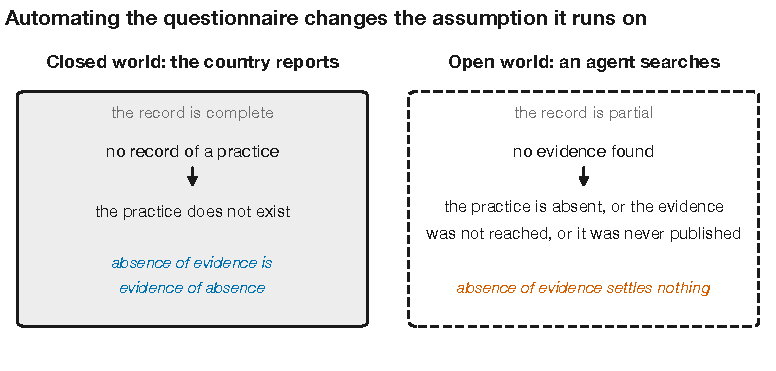
\includegraphics[width=\linewidth]{figures/fig_2_3_closed_vs_open_world.pdf}
\caption{The assumption the questionnaire runs on.}
\label{fig:assumption}
\end{figure}

Automating the questionnaire therefore changes the assumption it runs on. A country reporting on itself works under a \emph{closed world} assumption \citep{reiter1978}, where the data is full and complete, and absence of evidence of a practice equates to evidence of absence. An agent searching the open web, in the right-hand panel of Figure~\ref{fig:assumption}, has no such closure. When it finds no evidence for a practice, it cannot tell whether the practice is truly absent, or if it is just the evidence that is absent. That ambiguity makes proving a ``no'' difficult, and the system reflects this, with 87.0\% accuracy on the positive answers it commits to and 48.9\% on the negative ones (Section~\ref{sec:convergent-validity}).

\section{Approach}\label{sec:approach}

This dissertation builds and evaluates an agent swarm that answers the questionnaire from the open web. Three agents divide the work. A Researcher gathers evidence and proposes an answer. An adversarial Verifier then tries to refute that answer, searching for counterevidence, on the reasoning that opposition surfaces weak claims self-verification misses \citep{cohen2023}. Where the two cannot agree, an Adjudicator rules on the exchange. If there is an absence of substantive evidence, which may often be the case under an open world assumption, the system can also decline to answer.

The swarm is evaluated on a sample of eight of the thirty-six countries, 1,144 question-country pairs, scored against the published 2025 answers. It commits to an answer for 55.6\% of questions, agreeing with the key on approximately 70\% of those, and abstains on the remaining 44.4\%. Adding multiple agents roughly doubles the proportion of questions answered, with the number of correct answers improving similarly (Section~\ref{sec:ablation}). The premise that adversarial verification would perform better than a corroborative check did not hold. Changing the Verifier's stance leaves the results largely unchanged, consistent with recent literature. The benefit of debate appears to stem from an increased number of reasoning calls rather than from distinct stances, and varying the model may be more influential than varying the prompts \citep{chowdhury2026,zhu2026}. What bounds the system sits upstream of both, in what the open web holds, and no verifier can recover evidence that was never published. Consequently, its usefulness varies across the questionnaire, and Section~\ref{sec:reformulation} outlines a possible reformulation of the ODMI to facilitate the transition to automation.


\section{Research Questions}\label{sec:research-questions}

RQ1: Can an automated assessment meet the conditions that keep it legitimate?

RQ2: Is a swarm of agents with distinct roles more reliable in open-web retrieval than sole agents, and specifically, what is the added value of Adversarial Verification?

RQ3: What follows for the assessment itself? How much of the questionnaire can be delegated to the machine as it stands, and would the questionnaire have to be rewritten for the rest to be answerable from outside?


\section{Contributions}\label{sec:contributions}

The work makes four contributions. First, it assembles six criteria for judging a generative system that stands in for a human assessor. No framework for this yet exists \citep{unece2025}, so the criteria are drawn from a quality framework for statistical algorithms \citep{yung2022} and one for automated scoring \citep{williamson2012}, adapted to a system that also retrieves evidence. Second, it implements and documents a three-agent swarm that answers a policy assessment end-to-end, keeping a complete set of receipts for reproduction. Third, it reports an empirical test of adversarial debate where evidence is sparse, finding that the verification layer raises the share of questions answered from 26.6\% to 55.6\% whilst holding accuracy constant, and that what limits the system is the evidence the open web holds rather than the reasoning applied to it. Fourth, it turns towards the assessment, proposing how it could be reformulated to both be answerable from the web, whilst also becoming a better assessment of openness.

\section{Report Structure}\label{sec:report-structure}

Chapter~\ref{ch:background} introduces the index as a testbed, sets out the six criteria, and reviews the work on agentic retrieval, verification and abstention that the design draws on. Chapter~\ref{ch:methodology} describes the architecture and the evaluation design. Chapter~\ref{ch:results} reports the results from running the swarm through eight countries, taking the six criteria in turn. Chapter~\ref{ch:discussion} interprets the results, works through what can be delegated to an automated system, and develops the reformulation. Chapter~\ref{ch:conclusion} concludes.

\chapter{Background and Related Work}\label{background-and-related-work}

This section builds towards an architecture that can answer a policy questionnaire from the open web without asserting more than its evidence supports. It begins with the ODMI itself, followed by the criteria that must be met for it to remain a legitimate assessment post-automation. Past works are then weighed against those criteria. The review turns first to LLMs, why they are a sensible starting point and how they become agentic, then to the limitations that make them unreliable where evidence is scarce. Self-verification, multi-agent debate and abstention answer those limitations. The section closes with the difficulty a multi-lingual setting adds, and with the gap that remains for this work to address.

\section{The ODMI as an Assessment}\label{the-odmi-as-an-assessment}


\includegraphics[width=7.08611in,height=1.73819in]{/Users/benjyb/Desktop/MscProject/.claude/worktrees/odmi-figures-reconciliation-244489/Dissertation/latex/media/media/image2.png}

\ccnote{The four dimensions of the ODMI aim to measure} the entire open-data lifecycle, from creating policy to delivering real-world benefits. Policy measures open-data strategies, government structures, laws and implementation measures. Portal measures the functionality and usability of the national open data portal. Quality measures metadata standards, compliance, monitoring and data deployment quality. \ccnote{Impact measures the reuse of open data and the benefits it produces.} These dimensions perform sequential roles, with Policy informing decisions on open data, the Portal providing access to data, Quality assuring it is of a usable standard, and Impact measuring the value of this data.

A critique of the ODMI report is that it uses self-reporting by national open-data teams, which may lead to misinterpreted questions, reporting inconsistencies and self-reporting bias. The template for answers requests evidence but 15.1\% of the 5,148 pairs carry no comment at all, and if there is a populated comment it is frequently not evidence, such as a bare portal URL or one-word entries like ``yes''. Around 20\% of the questions cover internal practices (PT28 asks whether they monitor search key words, for example) and span all four dimensions. While Capgemini acts as an external verifier, they only change 10\% of the answers with counterevidence, complement the submitted answer with further evidence 27\% of the time, and confirm the original answer 63\% of the time.

Davis, Kingsbury and Merry (2012) argue that indicators, such as the ODMI, function as a technology of governance, ranking states, shaping standard-setting and influencing how resources are allocated and decisions are made. Their central concern is what reliance on indicators does to the authority and contestability of the decisions that follow. An indicator that has these influences must be open to scrutiny, and a country that disputes its ranking must be able to see the evidence upon which it was assessed. Contestability is the condition on which an indicator's legitimacy rests and is what a clear evidence trail supplies. On this reading, the ODMI's reliance on self-reporting means answers may rest on unevidenced or \ccnote{unverifiable assertions. 

Fumega and Gao (2026) put this directly, asking whether AI can take over indicator development, evidence discovery and policy evaluation without compromising `contextual nuance or democratic legitimacy' (p.1). Mirroring the results of human assessors is only half of the question. The other half is whether artificial intelligence can preserve the epistemic properties that make these assessments worth having, such as explainability.} Handing the job to a machine may cut costs, but if the underlying processes are opaque and indisputable, this technology ultimately degrades the authority and contestability of global benchmarking data \claudenote{(Davis et al., 2012)}.

\section{Criteria for an Automated System}\label{criteria-for-an-automated-system}

The criteria below set out what such a system has to demonstrate before it can be trusted with the automation of producing benchmarking indices. They govern any generative system that stands in for human judgement in producing a published assessment comparing several parties, where the system finds its own evidence. That covers the benchmarking indices in §2.1 and comparable exercises such as sustainability ratings and regulatory compliance monitoring.

The United Nations Economic Commission for Europe (UNECE) note that little specific guidance or established practice yet exists for using AI in generating official statistics and observe that most research remains focused on predictive rather than generative models (UNECE, 2025). No framework was identified during this work that lays out the criteria necessary for a reliable generative automation system. The criteria below are therefore assembled here, drawing on two established bodies of work with some adaptation to fit the setting.

Statistical agencies have for some time been automating work that people used to do by hand, and they have a settled way of deciding when that substitution is warranted. The Quality Framework for Statistical Algorithms (QF4SA) was published by the UNECE in 2022 (Yung et al., 2022) and was built with machine learning algorithms in mind. It directly addresses how previous statistical quality frameworks were written to judge a finished statistic, but not the algorithm that produced it, and they argue how an answer was reached is as important as the answer itself.

The QF4SA proposes five dimensions against which a statistical organisation should judge an algorithm before adopting it. Two of them, Cost and Timeliness, describe what an assessment costs to adopt and how quickly it runs, which are irrelevant to whether the process maintains legitimacy post-automation, so only three are carried forward here. Explainability is the degree to which a person can understand how an output follows from the inputs to it. Accuracy is the closeness of a computation to the value it was intended to measure. Reproducibility is the ability to obtain the same result from the same data and method. These dimensions are carried through, with explainability and accuracy extended into Attributability and Convergent Validity respectively, to reflect what they measure once the assessor is generative.

Williamson, Xi and Breyer (2012) set out the evidence an automated scorer must produce before it may be used operationally. Two of the criteria below come from their framework, Generalisability and Subgroup Equity, and a third shapes how accuracy is treated. \ccnote{Their framework was drafted for deterministic automated scoring of written answers.} It also assumes a human marks alongside the machine, and states that a machine marking alone would need stricter criteria than it currently supplies.

Convergent Validity asks whether the system reaches the right answer. The QF4SA defines accuracy as closeness to a true value, and \ccnote{§3.4} discusses the limits of self-reported answers as a stand-in for that value. Williamson et al. (2012) add that agreement with an independent measure carries more weight than agreement with a human key alone. Nine questions in the ODMI\textquotesingle s Quality dimension are deterministic, asking for a proportion of datasets meeting a metadata standard, and \ccnote{§3.5} sets out how these are computed directly.

\textbf{\ccnote{Table 2.1}: Criteria for a generative system automating an assessment.}

{\def\LTcaptype{none} % do not increment counter
\begin{longtable}[]{@{}
  >{\raggedright\arraybackslash}p{(\linewidth - 8\tabcolsep) * \real{0.1565}}
  >{\raggedright\arraybackslash}p{(\linewidth - 8\tabcolsep) * \real{0.1569}}
  >{\raggedright\arraybackslash}p{(\linewidth - 8\tabcolsep) * \real{0.2579}}
  >{\raggedright\arraybackslash}p{(\linewidth - 8\tabcolsep) * \real{0.2299}}
  >{\raggedright\arraybackslash}p{(\linewidth - 8\tabcolsep) * \real{0.1987}}@{}}
\toprule\noalign{}
\begin{minipage}[b]{\linewidth}\centering
\textbf{Criterion}
\end{minipage} & \begin{minipage}[b]{\linewidth}\centering
\textbf{What it asks}
\end{minipage} & \begin{minipage}[b]{\linewidth}\centering
\textbf{Why it matters here}
\end{minipage} & \begin{minipage}[b]{\linewidth}\centering
\textbf{What the system must show}
\end{minipage} & \begin{minipage}[b]{\linewidth}\centering
\textbf{Source, and what was adapted}
\end{minipage} \\
\midrule\noalign{}
\endhead
\bottomrule\noalign{}
\endlastfoot
Convergent Validity & Does the system reach the right answer? & The ODMI key is self-reported and can be a cycle old, so no single true value exists to score against (\ccnote{§3.4}). & Agreement with the ODMI key, and agreement with a measure computed independently of it. Nine Quality questions computed straight from catalogue metadata supply that second measure (\ccnote{§3.5}). & QF4SA accuracy (Yung et al., 2022). Williamson et al. (2012) add that an independent measure carries more weight than a human key alone. \\
Generalisability & Does performance hold across every kind of question the assessment requires? & An aggregate figure can be carried by the easy questions and hide failure on the rest. \claudenote{Running end to end over the open web, Fumega and Gao (2026) report mismatch against the human answers of 19\% on an indicator anchored in a single document against 69\% on one whose evidence is scattered, averaging 42\% over four indicators.} & Results decomposed by answer type and by ODMI dimension, not one headline figure. & Williamson et al. (2012). \\
Subgroup Equity & Are the countries being compared held to the same standard? & A country's score should follow from its open-data maturity, not from how searchable its web presence is or how well the model reads its language. & Adequate performance within each subgroup, not only overall, with results split by native language and maturity. & Williamson et al. (2012). Schenk and Kern (2024) extend QF4SA with algorithmic fairness, amending accuracy to require performance across subgroups. \\
Attributability & Does every committed answer trace to a passage a reader would agree supports it? & A generative model can produce a fluent answer with no basis (§2.4), and a country can only contest a score it is shown the evidence for. & Two conditions. The quoted passage exists in the cited source, and a reasonable reader agrees it supports the claim. & The QF4SA explainability (Yung et al., 2022), sharpened by the reader test in Rashkin et al. (2023). \\
Selectivity & Can the system decline to answer, and was it right to decline? & Models are optimised to guess when uncertain (Kalai et al., 2025). The QF4SA assumes the data is already available, but that is not the case for the ODMI, where the evidence has to be found and may not exist in public. & A commitment only where the evidence supports it, an abstention otherwise, and a stated confidence that tracks observed accuracy. & New here. Neither framework supplies it, as both assume a system that always answers. \\
Reproducibility & Does a second run of the assessment return the same answers? & A deterministic algorithm satisfies this by construction and a generative assessor cannot. Two runs may search differently while the truth has not changed, so the outcome is what has to hold, not the route. & Traceability, a property of the record: prompts, evidence, model version and settings, enough to re-derive any reported figure without re-running the system. Stability, a property of the system, measured as variance between runs. & QF4SA reproducibility (Yung et al., 2022), the one dimension carried through unchanged. \\
\end{longtable}
}

Together these six criteria\claudenote{, set out in Table 2.1,} make up the conditions under which an automated ODMI score remains contestable in Davis et al.\textquotesingle s sense. A country disputing its score should be able to check the evidence held against it (Attributability), and know the answers weren't guessed (Selectivity). It should also be able to establish whether the same standard was applied to its neighbours (Subgroup Equity), whether the result agrees with what a human assessor would have reached (Convergent Validity), whether the score rests on the parts of the questionnaire the system handles best (Generalisability), and whether a second run would return the same figure (Reproducibility).

\section{Limitations of LLMs in Truth-Seeking}\label{limitations-of-llms-in-truth-seeking}

Using a basic large language model in an evidence-retrieval setting has two key drawbacks. It can only recall information from its training data, and this information isn't necessarily true. LLMs are optimised to match the statistical distribution of their training corpus, so the gradient signal rewards predicting the most likely next token based on context, not factual truth. Truth only enters indirectly; the phrase ``the capital of France is'' is most likely followed by ``Paris'', as this is the most frequent resolution of the sentence, not because it `knows' that is the case. The training objective never targets truth directly; it is a byproduct of statistical patterns in text. Figure\,2.1 illustrates that, in the long tail where facts are rare in the training corpus, completing a statement may result in many continuations, not all of which are true (Kandpal et\,al.,\,2023). Backpropagation preserves the statistical regularity of a fact while discarding its provenance, so the model retains that a completion is likely but not where it came from or how reliable that source was.


\includegraphics[width=5.9in,height=2.26898in]{/Users/benjyb/Desktop/MscProject/.claude/worktrees/odmi-figures-reconciliation-244489/Dissertation/latex/media/media/image3.png}

\ccnote{Figure 2.1: Why the objective produces hallucination. }

A model built this way will therefore state things that are false, and will state them as confidently as it states things that are true. A pertinent question is why the behaviour survives post-training, where reinforcement learning shapes the model towards answering in a desired manner rather than merely fluently. Most benchmarks are graded binarily and award no credit for abstention, so a model answering "I do not know" scores identically to one answering incorrectly, while a model that guesses has positive expected value (Kalai et al., 2025). Optimisation against such benchmarks actively encourages confident fabrication under uncertainty, since the chance of guessing correctly is non-zero and the chance of scoring by abstaining is not. This incentive is inherited by any system built on such a model.

\emph{Extrinsic} hallucination is the main risk for the purposes of agentic research, where the generated output cannot be verified from the source (Maynez et al., 2020; Ji et al., 2023). Previous works in retrieval-augmented generation and web retrieval systems have constrained models to reason solely from web-derived evidence, treating parametric recall as inadmissible (Lewis et al., 2020; Nakano et al., 2021; Menick et al., 2022; Gao et al., 2023). 
\includegraphics[width=7.08611in,height=3.24167in]{/Users/benjyb/Desktop/MscProject/.claude/worktrees/odmi-figures-reconciliation-244489/Dissertation/latex/media/media/image4.png}

\ccnote{Figure 2.2: Prior-steered retrieval. }

The constraint is not airtight\textbf{\ccnote{, as the loop traced in Figure 2.2 shows, since}} parametric knowledge cannot be switched off and models tend to resolve conflicts between retrieved context and prior belief in favour of the prior (Longpre et al., 2021). \ccnote{The no-retrieval baseline is reported in Table F.1}, to isolate the effect of prior steering. The failure mode that dominates in this setting, however, comes from the ODMI's sparse evidence. Much of what the questionnaire asks about exists only in obscure national portals, in inconsistent formats, and in some cases nowhere public at all, which is the long-tail regime in which a model\textquotesingle s recall is least reliable (Mallen et al., 2023). A search over that space often returns a document on the same subject as the question, but that does not directly settle it. The agent then has to decide whether such a document supports its claim, and it decides under the incentive set out above, where committing scores and abstaining does not. The dominant failure is therefore over-reading, where the system treats related evidence as proof of the claim. Every citation it offers is real, so requiring the agent to cite its sources does not catch it.

A ``yes'' is an existential claim, and one document that establishes the practice discharges it, so retrieval is the right instrument for reaching it. A ``no'' on a question asking whether a portal feature exists is settled by inspection, because the search space is bounded and the agent can look at the portal and see. A ``no'' about a team\textquotesingle s internal practice is not, because the practice leaves no public trace, and finding nothing cannot separate a practice that is absent from evidence the agent did not reach.\\
\strut \\
§1.3 set this out as the move from the closed world a country reports under to the open world the agent searches (Reiter, 1978). The consequence for an agent under the guessing incentive runs one way. Weak evidence can be misinterpreted as a ``yes'', while little can be misinterpreted as a ``no'', so the system commits on weak support in one direction and withholds a correct answer in the other. This highlights the need for abstention, allowing the system to decline answering when the retrieved evidence is insufficient to support the claim.

Meeting the Selectivity standard set out in §2.2 requires three things of the architecture. The system has to be able to interrogate its own outputs, to subject them to adversarial challenge, and to return nothing at all where the evidence does not reach. The remainder of this chapter takes each in turn, \claudenote{self-verification in §2.4, adversarial multi-agent debate in §2.5 and abstention in §2.6}.

\section{Methods towards Verification}\label{methods-towards-verification}

\ccnote{Figure 2.3 traces the lineage between the past works, where no single work arrives at the set of requirements the ODMI requires.}


\includegraphics[width=5.4in,height=3.69858in]{/Users/benjyb/Desktop/MscProject/.claude/worktrees/odmi-figures-reconciliation-244489/Dissertation/latex/media/media/image5.png}

\ccnote{Figure 2.3: What each prior method adds and misses}

SelfCheckGPT (Manakul et al., 2023) samples the same response several times and measures how far the responses agree, on the finding that hallucinated content diverges under resampling while well-attested content does not. Dhuliawala et al. (2024) take an adjacent route, drafting an answer, breaking it into atomic verification questions, and answering each without the draft in view so the original claim cannot steer the check. They note that retrieval-based systems beat their architecture on very rare facts, which \claudenote{ties back to the long-tail argument in §2.3}. Both works improve accuracy over answering directly, and both share one error. They detect inconsistency within prior knowledge and say nothing about whether that prior knowledge is correct. Neither consults an external source, so both fail on Attributability with no evidence trail beyond the model\textquotesingle s own parameters.

Intrinsic self-correction fails to improve reasoning, and sometimes degrades it \ccnote{(Huang et al., 2024).} This is because the bottleneck is not error \emph{correction}, but error \emph{detection} (Tyen et al., 2024). If a model cannot detect its own error, then \claudenote{asking} the same model to check for it will miss the same blind spot. Furthermore, intrinsic self-correction may bolster \claudenote{the model's self-confidence} \ccnote{(Simhi et al., 2025)} in its answers regardless of whether the claim \ccnote{is true, degrading Selectivity}. This points towards needing an external knowledge base to fact-check claims before submission.

SAFE (Wei et al., 2024) decomposes a response into individual atomic claims, running an iterative search-and-reason loop over each claim and issuing its own follow-up queries before rating it ``supported'' or ``not supported''. This method passes Attributability, as it consults external evidence and \ccnote{ties each claim to a cited source. It fails} Selectivity because SAFE has no confidence output and no way to return nothing. The authors state that SAFE "does not assess the global accuracy of a fact" (p.28). A claim the search finds no evidence for is rated not supported, \ccnote{the same as a claim the search finds contradicting evidence for.} Absence of evidence becomes evidence of absence, which is the closed-world assumption §1.3 rules out.

The deeper limitation is the direction of the search. SAFE generates its queries from the claim in order to verify it, so the evidence it gathers is selected for proximity to the claim before anything is judged, and no step goes looking for material that would contradict it. The authors concede the consequence, that SAFE "may find supporting information for a factually inaccurate fact" (p.28). Nothing at the rating step corrects for this, because the model must return supported or not supported with no way to say it cannot tell. \claudenote{That is the binary grading §2.3 described}, where a model does better by guessing than by acknowledging uncertainty (Kalai et al., 2025). The ODMI setting may exacerbate this issue, because a question concerning obscure national data can be surrounded by ample publicly available adjacent evidence, yet fail to establish the data directly, and a verifier seeking only support may interpret the proximity as confirmation.

\ccnote{This motivates the question this work puts to test, whether opposition} is what a setting with little to no evidence requires. If one agent is tasked with defending a claim, and one with refuting it, the model's disposition to confidently assert is set against itself instead of being left to run in the same direction, meaning only claims backed by substantial \claudenote{evidence should survive the process}. This results in three relations. The claim survives refutation, the refutation defeats the claim, or both positions are asserted equally with opposing evidence. \ccnote{It is} this third relation \ccnote{that a single corroborative check cannot resolve and is most significant} in an environment where sparse and adjacent evidence is expected.\ccnote{ Whether the opposition itself does the work, or the extra retrieval that arguing forces, is what }\claudenote{§4.7}\ccnote{ separates.}

\section{Multi-Agent Debate for Verification}\label{multi-agent-debate-for-verification}

Multi-agent adversarial verification sits within the multi-agent debate family and is a relatively new line of research. Du et al. (2023) proposed a collaborative multi-agent architecture and found that cooperatively proposing and critiquing arguments meant the agents' collective intelligence could self-correct hallucinations. Liang et al. (2023)\claudenote{ are among the first to shift away from} collaborative debate, towards using adversarial tension to expose weak reasoning. \claudenote{§2.4 showed that a model cannot reliably check itself}, since it carries the same blind spots that produced the error (Huang et al., 2024; Tyen et al., 2024). A second agent set to agree inherits the problem and adds little in a data-scarce setting. Cohen et al. (2023) found that opposition surfaces errors a corroborative check misses, though their verifier interrogated the claim alone and admitted no external evidence. The hypothesis here is that adversarial pressure decorrelates the two models\textquotesingle{} errors, and that pairing that pressure with retrieval closes the gap Cohen left open.

If model A (the Researcher) is tasked with proving a claim, it is optimised to assert over abstaining (Kalai et al., 2025) and may retrieve some tangential evidence that proves an adjacent claim because no direct evidence exists on the web. Model B (the Verifier) is tasked with finding a flaw in model A's argument, and this weak reasoning should be surfaced. Note this decorrelation is only partial since A and B may share weights and priors, relevant here as this work uses the same Claude model for all agents. A and B argue their case over sequential rounds, gathering new evidence for each round, and if no agreement is reached this transcript is given to model C (the Adjudicator), which is comparatively reliable at correcting logical inconsistencies once their location is supplied (Tyen et al., 2024), as each agent has pointed out each other's weak reasoning.

Chowdhury et al. (2026) are the closest architectural precedent. Their PROClaim framework creates a judicial process for multi-agent debate, with evidence admission protocols and multi-stage deliberation, and it improves on standard multi-agent debate by 10.0 points. Each of their three judges runs a different underlying model, on the argument that agents drawn from the same weights share representations and cannot be relied on to disagree. Their own ablation puts the largest single share of the gain, 7.5 points, on progressive evidence retrieval. The argumentation structure accounts for less. Removing progressive retrieval raises agreement between their judges while accuracy falls. They read that rise as convergence without correctness, an ``epistemic bubble'', which is the failure a corroborative check produces on thin evidence. A single-call model with retrieval still beat the full courtroom on raw accuracy, 85.8\% against 81.7\%, however the same single model argued opposing conclusions convincingly from one evidence pool. An answer that cannot be audited is worth less than one that can, whatever it scores, and Chowdhury et al. rest their contribution on traceability and calibration rather than accuracy. They report an expected calibration error of 0.034, which addresses the second condition of Selectivity directly. It comes from a cross-validated grid search over one parameter, the weight on judge consensus in their confidence score, and their accuracy is unchanged at either setting, so the calibration rescales confidence without moving a verdict.

Smit et al. (2024) found that debate protocols do not reliably outperform cheaper strategies such as self-consistency and `multi-path ensembling'. Zhu et al. (2026) set out the sharper condition, showing that where agents are homogeneous and both are equally likely to be right, debate preserves expected correctness and cannot improve on majority vote. That applies here, since the Researcher and the Verifier are one model separated by a prompt. The result assumes a pool of evidence that stays fixed for the duration of the exchange, and each round here retrieves new material, which is the same mechanism Chowdhury et al. (2026) measured when progressive retrieval carried 7.5 of their 10.0 points. \ccnote{The claim under test is therefore narrower than ``debate is unanimously better''. It is that adversarial debate over retrieved evidence separates from a corroborative check in a sparse-web environment, whether on accuracy or on false positives. }\claudenote{§4.7}\ccnote{ settles it by ablating each agent in turn.}

\section{Allowing for Abstention}\label{allowing-for-abstention}

\claudenote{§2.5 left the system with three outcomes}. Debate can settle which of two cases has stronger evidence, but it cannot settle a case where the evidence is equally weak on both sides. Embedding a model in a debate \claudenote{does not remove the guessing incentive of §2.3}, and both Researcher and Verifier will guess if forced to produce an answer. Abstention removes this pressure. Where a question measures an internal practice, or little to no evidence exists online, abstention is what lets the system decline honestly.

One way to trigger it is to have the agent assign a confidence score to its argument and let a threshold decide when to abstain. It is much simpler to ask the agent to rate how well its retrieved evidence supports the claim, than it is to get it to refuse to answer outright due to insufficient evidence. Generating a confidence score demands the agent weigh up the relation between two pieces of text, whereas expecting it to self-regulate goes against its engrained guessing incentive. The decision to withhold then belongs to the threshold, and the agent is never asked to refuse.

When a model commits with confidence 0.7 it should be correct roughly 70\% of the time, but the score is self-declared, and nothing makes it track truth. Calibration is therefore assessed after the run, from the confidences the system logged. \ccnote{§3.9} defines the measure and \claudenote{§4.2} reports it. Feng et al. (2024) show calibrated abstention is achievable in multi-agent collaboration, reporting an abstain expected calibration error for their collaborative approaches. They also find models abstain less when predicting future election outcomes for African and Asian countries, which they read as a fairness concern for abstention mechanisms. Theirs is the only work in this chapter to address Selectivity and Subgroup Equity together.

Abstention has a hidden cost, as while the system declining is what stops it guessing, a declined question is still a question the assessment has no answer for. This means total accuracy reduces as abstention increases, and a system maximising accuracy just on answers it commits is incentivised to answer extremely cautiously. And thus, the choice of threshold is a policy decision, balancing coverage and accuracy. Selectivity from §2.2 asks both whether the system can decline and whether it was right to do so. The design supplies the first. Calibration is what would make the stated confidence non-trivial, and \claudenote{§4.2} reports whether it did.

\section{Multilingual Evidence Retrieval}\label{multilingual-evidence-retrieval}

The ODMI covers thirty-six states and more than twenty languages, and any variance in how well the system assesses them lands directly on Subgroup Equity. When a state scores poorly, three explanations sit behind that score, since the model may have misunderstood the evidence, the evidence may never have been published, or the country may simply be less open than its peers. Only the first is a property of the assessor rather than the country, which makes comprehension the one artefact that can and should be isolated.

Language capability is not uniform, because an LLM acquires each language as a by-product of next-token prediction and therefore in proportion to how often that language appeared in its corpus. Thellmann et al. (2024) evaluated forty LLMs on translated benchmarks across twenty-one European languages, and for LLaMA-3.1-70B-Instruct average accuracy falls from 0.79 in English to 0.66 or below for Estonian, Latvian and Lithuanian, declining with each language\textquotesingle s share of CommonCrawl's web archives. Anthropic\textquotesingle s own card shows the same trend inside the Claude family, with Sonnet scoring 69.0\% on the translated MMLU against 79.0\% on the English original (Anthropic, 2024).

Isolating comprehension does not clear Subgroup Equity on its own. Countries differ in what they publish, how they publish it, and how easy their national estates are to browse, so lower maturity may itself confound the ability for the system to assess their score. Separating them is what \claudenote{§4.4} attempts to do.

\section{Research Gap}\label{research-gap}

Two lines of work run through this chapter. One gives a model the means to retrieve its own evidence and act on it, the other checks whether an answer is sound. The two works that come closest to joining them are set out below, before \ccnote{Table 2.2} scores every work in the chapter against the six criteria.

Yao et al. (2023) interleave reasoning and action in their ReAct framework, alternating a thought, an action, and an observation of what that action returned, so that reasoning decides what to retrieve and what comes back shapes the next thought. The alternation leaves a legible record of each thought, the action it led to and what that action found, which is Attributability in principle. However, it does not provide verification. The loop ends once the agent judges it has an answer, so nothing in the architecture ensures the output is correct.

The closest analogue to this paper's work is Fumega and Gao (2026), who test commercial deep-research agents against the Global Data Barometer questionnaire, an assessment similar to the ODMI. A deep-research agent takes a question, runs its own searches, reads what it finds and returns a report with a list of sources. In their work, an agent finds the evidence itself and then answers from it, and they report an average match of 58\% against the human answers over four indicators. That runs from 81\% on Data Protection, whose evidence sits in a single legal document, to 31\% on Land Tenure, whose evidence is scattered across separate land management systems. They also identified cases in which the agent's answer was more accurate than the expert's, and whether a similar premise holds in the ODMI's case is taken up in \claudenote{§5.3}.

Their work highlights the necessity of both conditions of Attributability, as the agents are asked for citations and supply them, per sub-question with a working link, but nothing checks that the citation supports the claim. They cite such failures, e.g., an ``API Access'' button that did not function, as evidence without testing it. They have no independent computable measure to anchor Convergent Validity either, of the kind the nine computable ODMI questions provide. Subgroup Equity is raised and left untested, and there is no abstention channel or calibrated confidence.

Appendix E details how these works score against the full criteria.

\section{}\label{section-6}

{\def\LTcaptype{none} % do not increment counter
\begin{longtable}[]{@{}
  >{\raggedright\arraybackslash}p{(\linewidth - 12\tabcolsep) * \real{0.1639}}
  >{\raggedright\arraybackslash}p{(\linewidth - 12\tabcolsep) * \real{0.1382}}
  >{\raggedright\arraybackslash}p{(\linewidth - 12\tabcolsep) * \real{0.1394}}
  >{\raggedright\arraybackslash}p{(\linewidth - 12\tabcolsep) * \real{0.1393}}
  >{\raggedright\arraybackslash}p{(\linewidth - 12\tabcolsep) * \real{0.1415}}
  >{\raggedright\arraybackslash}p{(\linewidth - 12\tabcolsep) * \real{0.1395}}
  >{\raggedright\arraybackslash}p{(\linewidth - 12\tabcolsep) * \real{0.1382}}@{}}
\toprule\noalign{}
\begin{minipage}[b]{\linewidth}\raggedright
\textbf{Work}
\end{minipage} & \begin{minipage}[b]{\linewidth}\raggedright
\textbf{Conv. Validity}
\end{minipage} & \begin{minipage}[b]{\linewidth}\raggedright
\textbf{Generalis.}
\end{minipage} & \begin{minipage}[b]{\linewidth}\raggedright
\textbf{Subgroup Equity}
\end{minipage} & \begin{minipage}[b]{\linewidth}\raggedright
\textbf{Attributability}
\end{minipage} & \begin{minipage}[b]{\linewidth}\raggedright
\textbf{Selectivity}
\end{minipage} & \begin{minipage}[b]{\linewidth}\raggedright
\textbf{Reprod.}
\end{minipage} \\
\midrule\noalign{}
\endhead
\bottomrule\noalign{}
\endlastfoot
ReAct (Yao et al., 2023) & Partial & Partial & ✗ & Partial & ✗ & Partial \\
SelfCheckGPT (Manakul et al., 2023) & Partial & ✗ & ✗ & ✗ & Partial & Partial \\
Chain-of-Verification (Dhuliawala et al., 2024) & Partial & Partial & ✗ & ✗ & ✗ & Partial \\
LM vs LM (Cohen et al., 2023) & Partial & Partial & ✗ & ✗ & ✗ & Partial \\
Du et al. (2023) & Partial & Partial & ✗ & ✗ & ✗ & Partial \\
Liang et al. (2023) & Partial & ✗ & ✗ & ✗ & ✗ & Partial \\
Smit et al. (2024) & Partial & Partial & ✗ & ✗ & ✗ & Partial \\
Zhu et al. (2026) & Partial & Partial & ✗ & ✗ & Partial & Partial \\
SAFE (Wei et al., 2024) & ✓ & Partial & ✗ & ✓ & Partial & Partial \\
Feng et al. (2024) & Partial & Partial & ✓ & Partial & ✓ & Partial \\
Chowdhury et al. (2026) & ✓ & ✓ & ✗ & ✓ & ✓ & ✓ \\
Fumega and Gao (2026) & ✓ & ✓ & ✗ & Partial & ✗ & Partial \\
This work & ✓ & ✓ & ✓ & ✓ & ✓ & ✓ \\
\end{longtable}
}

\ccnote{Table 2.2}: Prior work scored against the six criteria of §2.2. A tick means the work addresses and reports the criterion, not that it succeeds. Partial means it addresses one of the criterion\textquotesingle s two conditions, or reports it without measuring it. The full justification for every cell, with the passage each verdict is read from, is in Appendix E.

\ccnote{Table 2.2} shows the shape of the gap. Attributability and Selectivity are met together only by Chowdhury et al. (2026). The only system operating in a real assessment setting, Fumega and Gao (2026), satisfies neither of the criteria fully. Although commercial research agents leave a per‑claim trail, they lack a method to verify that the cited source supports the claim, and they have no abstention channel. The verification machinery and the open-world setting have never been brought together.

Two columns of the table are close to empty. Only Chowdhury et al. (2026) test whether a generative assessor returns the same answers on a second run, reporting performance across three independent runs and conceding that run-level variance remains notable. Every other work states its decoding settings without ever repeating a run. Subgroup Equity has one entry. Feng et al. (2024) split their election set by region and found abstention rates lower for Africa and Asia, which they read as a fairness problem in abstention itself. That is the only prior measurement of whether such a system treats its subjects evenly, and \claudenote{§4.4} analyses how abstention varies within the subgroups.

This paper takes adversarial verification into that setting. A Verifier hunts for counterevidence, so a committed answer has had to survive an active attempt to refute it before an Adjudicator settles the case. Abstention is a first-class output, calibrated on confidence scores, so that thin evidence produces a withheld answer. The design targets the two criteria corroborative systems miss, namely Attributability, where every committed answer traces to a passage that entails it, and Selectivity, where stated confidence tracks truth and the system can decline. The remaining four criteria from §2.2 test whether the system succeeds, with Convergent Validity tested against the human key and against an independent recompute, Reproducibility upholding strict receipt taking and tracking stability across multiple runs, and Generalisability and Subgroup Equity looking across a decomposition by dimension and country.


\chapter{Approach and Methodology}\label{approach-and-methodology}

§2 set out the six criteria an automated assessor has to meet. This chapter describes the system built around them and the design used to test it. The first four sections cover the architecture, taking the three agents and the loop they run, then the search pipeline that feeds them evidence, then the deterministic route that computes the nine catalogue questions from harvested portal metadata. The next three cover the evaluation design. They establish the ODMI answer key as the comparator and set out where it is weak, define the eight sampled countries for the final run, and define the measures each result is reported under. The last two sections deal with the controls placed on data leakage and the method behind the experiments.

\section{System Architecture}\label{system-architecture}

The architecture opposes a Researcher agent with an Adversarial Verifier whose job is to disprove, so claims are scrutinised alongside their evidence before they are committed. This adversarial pressure addresses the guessing bias that corroborative checks are vulnerable to, as §2.2 laid out. A second agent asked to confirm findings will tend to ratify a plausible answer, whereas an agent asked to refute aims to produce grounds to do so. A third agent, the Adjudicator, resolves unsettled cases and may decline to answer where neither position prevails.

Requiring the Researcher to return a verbatim passage forms the first half of Attributability, showing exactly where the evidence comes from. The Verifier\textquotesingle s judgement of evidence fit stands in for whether a reasonable reader would agree it entails the claimed answer, so a quote that is real but does not support the label is refused. The Adjudicator\textquotesingle s capacity to abstain is the architecture\textquotesingle s provision for Selectivity, and the thresholds that govern it are set out in §3.2. Every model call writes a record of the model used, the prompt version, the input and output token counts, the latency and the cost, so that any result can be reconstructed from the logged data alone. That record is the traceability half of Reproducibility; the stability half cannot be built in and has to be measured, which §4.6 does. Subgroup Equity and Generalisability are properties of the evaluation rather than of the architecture, and are treated in §4.4 and §4.5 respectively. Nine Quality questions bypass the agents entirely. A deterministic tool computes the figure straight from portal metadata, with no model involved. That gives Convergent Validity a measure that does not rest on the human key, and §3.5 sets out how it works.

\section{The Agent Loop}\label{the-agent-loop}

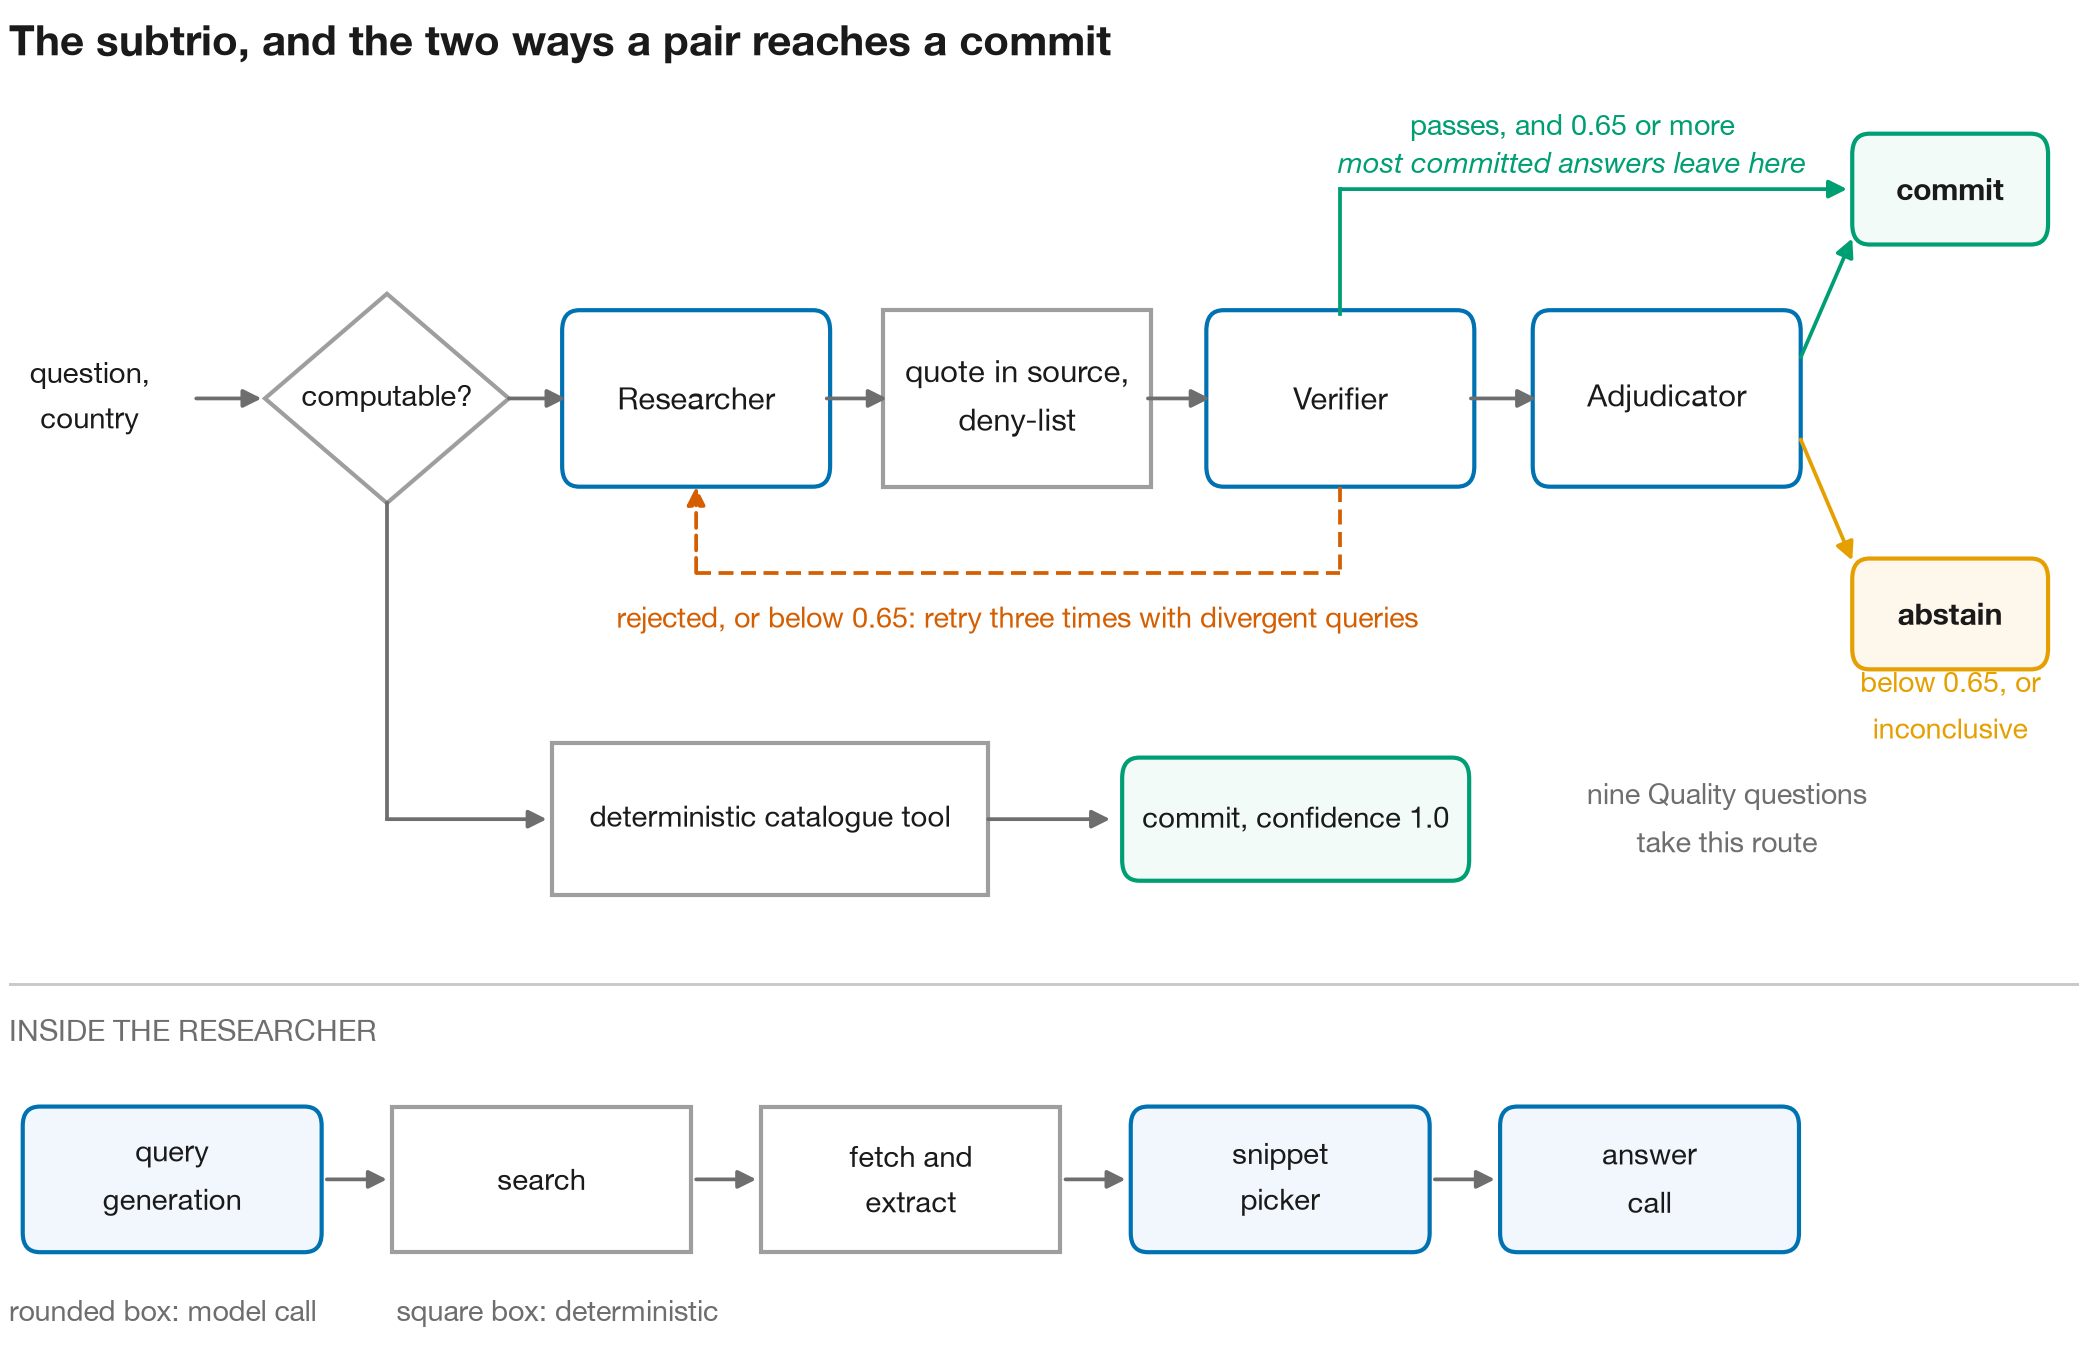
\includegraphics[width=7.08611in,height=4.60208in]{media/media/image6.png}

Figure 3.1: The three agent swarm.

A pair either routes to the deterministic catalogue tool or through the three agents, and reaches a commit by one of two paths.

The Researcher: The first of three model calls converts the question and country into two or three brief search queries, one in English and, if the national language differs, one in that language. The second reads each page the pipeline fetches and keeps the passages relevant to the question, dropping any page that yields none. The third reads the snippets it kept and generates a structured answer comprising a label, a verbatim passage, the source URL, and two confidence scores: one for the evidence found and one for the answer derived from that evidence. The quote and URL make the answer auditable, and the answer confidence is the score the commit threshold acts on.

The Verifier: the verification system comprises several deterministic and probabilistic components. It begins with a deterministic offline gate that checks whether the cited quote appears in the snippet and whether the URL is absent from the deny-list of §3.6. The gate is deliberately lenient in three recorded ways, set out in Appendix B. The system seeks reasons to reject the Researcher\textquotesingle s claim, proceeding through five reasoning steps: substring check, source authority, evidence fit, counterevidence, and verdict. It also conducts an adversarial counter-search for every question, on queries a small model call of its own generates. If the Verifier accepts the answer and the Researcher\textquotesingle s confidence exceeds the final threshold, the pair proceeds to the upper exit shown in Figure 3.1, without an Adjudicator pass. Otherwise, the Verifier returns its counter-argument to the Researcher for a retry.

Commit: If the Verifier passes the answer and the Researcher confidence clears the final floor, the pair commits there, with no Adjudicator pass. Most committed answers leave the loop at this point.

Retry: a rejected or sub-floor answer returns to the Researcher with the Verifier\textquotesingle s counterevidence attached, and the next attempt is forced to diverge from the queries already tried. Without that constraint the retry re-reads the pages that produced the rejected answer, so the loop repeats itself rather than reaching new evidence. Each round therefore enlarges the evidence pool rather than re-arguing over a fixed one. That is the progressive retrieval §2.5 identified as carrying most of Chowdhury et al.\textquotesingle s improvement. Three retries are allowed, so four attempts in all.

The Adjudicator: Only once the retry loop is exhausted, the Adjudicator agent is deployed. It runs no new web searches, and weighs up all the collected evidence throughout the retries from both previous agents. It outputs an authoritative verdict on whether the Researcher, the Verifier or neither was correct, or that the case cannot be settled at all, together with an answer, a confidence, a reasoning string, and the source URL and quote it commits to. If the Adjudicator confidence is below the threshold the answer is not committed.

Confidence threshold: A single threshold governs commitment, 0.65. A Verifier finalises an answer only if the label is not an abstention and the Researcher\textquotesingle s confidence reaches 0.65; otherwise, the pair returns to the retry loop. The same threshold is applied after adjudication, where an Adjudicator answer below 0.65 is rewritten as inconclusive. As detailed in §2.6, the choice of threshold is a policy decision, between balancing accuracy and coverage.

\section{Retrieval}\label{retrieval}

The success of the Researcher depends entirely on the quality of information it can reason over, and as such the search pipeline requires as much thought as the swarm architecture. When the Researcher receives the question-country pair, an LLM call generates three likely search queries that may surface the answer, one in English, an optional native-language query, and an optional query aimed at the national portal. The native-language query exists to surface sources an English query would miss.

The pipeline then runs in stages. Each query is issued to a Google Serper search returning five results. Each result is fetched over httpx, with a Playwright fallback for pages that time out, return an error, or render their content through JavaScript or a web-application firewall. The fetched page is reduced to its main text with the trafilatura Python library, and this extracted text, capped at 16,000 characters, is passed to a Claude snippet picker. The picker scores the candidate passages and returns them ranked best-first. Where one passage clearly dominates it returns that alone; otherwise it returns up to three, each held to 500 characters. The passages taken from a page are then joined into a single snippet, so a three-passage pick runs up to 1,500 characters. At answer time every snippet is truncated to 600 characters before entering the Researcher\textquotesingle s prompt, and up to fifteen snippets reach the answer call. Because the picker ranks passages best-first, this cap retains the strongest evidence and drops a lower-scored tail. That tail is relevant enough to be selected but is the likeliest source of the weak quotes an answer wrongly settles on, and the cap also shortens the run. The pipeline caches at three levels, the search result, the page fetch and the picked snippet, each for thirty days, so that repeated runs are reproducible and cheap. 

\section{Ground Truth and Its Limits}\label{ground-truth-and-its-limits}

The swarm\textquotesingle s accuracy is marked against the 2025 ODMI assessment answers, as it is the closest publicly available ground truth. It provides all 5,148 answers across every question-country pair, each one self-reported by the country and then reviewed by Capgemini, who confirm 63\% of answers, supplement 27\% of answers with more evidence, and actively change around 10\%. The evidence attached to an answer ranges from a clear URL to a more informal comment from a national data team such as \textquotesingle We are working on it\textquotesingle. In §4, the term `gold' refers to the answer in the ground truth set, for example `negative-golds' means the questions in the 2025 questionnaire that were answered with a ``no'' or low band. Table 3.1 shows the breakdown of question type, with the majority requiring a binary answer.

{\def\LTcaptype{none} % do not increment counter
\begin{longtable}[]{@{}
  >{\raggedright\arraybackslash}p{(\linewidth - 4\tabcolsep) * \real{0.5000}}
  >{\centering\arraybackslash}p{(\linewidth - 4\tabcolsep) * \real{0.2500}}
  >{\centering\arraybackslash}p{(\linewidth - 4\tabcolsep) * \real{0.2500}}@{}}
\toprule\noalign{}
\begin{minipage}[b]{\linewidth}\raggedright
\textbf{Answer shape}
\end{minipage} & \begin{minipage}[b]{\linewidth}\centering
\textbf{Count}
\end{minipage} & \begin{minipage}[b]{\linewidth}\centering
\textbf{Share}
\end{minipage} \\
\midrule\noalign{}
\endhead
\bottomrule\noalign{}
\endlastfoot
Binary (yes / no) & 124 & 87\% \\
Percentage-band & 12 & 8\% \\
Ordinal-magnitude & 3 & 2\% \\
Count-band & 2 & 1\% \\
Categorical & 2 & 1\% \\
\textbf{Total} & \textbf{143} & \textbf{100\%} \\
\end{longtable}
}

Table 3.1: Answer shapes across the 143 questions.

Rating accuracy as the match rate with this ground-truth is not perfect. The answers originate with the country, and 29 of the questions ask about internal practice where evidence is hard to find online, such as \textquotesingle Do you monitor search keywords?\textquotesingle{} or \textquotesingle Do you monitor portal traffic?\textquotesingle (Appendix D lists all 29). Across all 36 countries these 29 questions are answered ``yes'' 79.3\% of the time, which confounds whether the system is successfully retrieving the relevant information and reasoning carefully over it, or whether the architecture has not addressed the natural LLM optimism bias and both Researcher and Verifier have been misled by vague or missing evidence. This points to a class of error that sits outside the declared ground-truth mismatches, and isolating it is an necessary step towards true reliability. Secondly, many of the calculated answers for the nine deterministic questions diverge from the reported figures, as shown in §3.5, so the ground truth is demonstrably wrong on at least some items. 

These two flaws change how the evaluation has to be framed. Where the swarm and the ODMI disagree, it can be unclear whether the swarm is wrong or the ODMI is, and Fumega and Gao (2026) found that an agentic assessor is sometimes right where the human experts are not. Neither rater is infallible here, since the swarm can misread evidence and the human key is self-reported and diverges from the recompute. §4.1 takes this up again, doing an independent audit of 94 false positives across eight countries, to see where the system falls short, and which questions are structurally out-of-reach for a closed-world assessment.

\section{Deterministic Tool for Catalogue Questions}\label{deterministic-tool-for-catalogue-questions}

Nine Quality questions ask for a proportion of the national catalogue, for example the share of datasets conforming to DCAT-AP, which is directly computable. The only pooled public source for the same figures is the Metadata Quality Assessment (MQA) on data.europa.eu, which is deny-listed because that domain also publishes the assessment\textquotesingle s own answers. A deterministic tool computes them instead, with no language model involved at any stage.

Each catalogue question asks a national team to select a percentage band for its own portal, that band carries a score, and Capgemini confirms or amends what the team submits. Across the thirty-six countries the key records 280 confirmations against 44 amendments, so in every case there was a submitted answer for a reviewer to rule on. The self-report shows plainly wherever a team was challenged, with countries defending their own portal in the first person, several replying directly to a reviewer\textquotesingle s remark, and one answering ``i don\textquotesingle t know''. Two national teams cite the MQA as the basis of their numbers. What sits behind the rest is thinner. Of the 324 rows, 87 leave the evidence box empty and a further 207 carry only the string `N/A', so nine in ten offer nothing to check, and 86\% were confirmed with no amendment. On this group the assessment accepts a self-reported figure with nothing attached to support it.

The tool can only harvest a country whose portal route is known, so classification comes first. A stack-fingerprinting prober covering CKAN, uData, paged DCAT-AP, SPARQL, piveau, OpenDataSoft and data.json portals identifies each national portal and records the route in a registry, verified against a one-page sample before the route is trusted. 22 of the 36 countries carry a registry entry. The harvester then pages the catalogue and stores the retrieved metadata as a snapshot with a SHA-256 of its contents, and the nine metric functions run over that stored snapshot. Conformance is scored against the SEMIC DCAT-AP SHACL. Nine countries hold at least one complete snapshot, and several harvests failed part way and are flagged as partial, most often on a read timeout or a DNS error. The recompute in Table 3.2 exposes gaps in the self-reported figures, running in both directions. France reports over 90\% licence coverage against a recomputed 37.8\% over a sample of five thousand datasets. Romania reports 10-30\% on recommended DCAT-AP property usage and under 10\% on optional usage, against a recompute of 100\% and 99.7\%.

Table 3.2: Full and sampled harvests of national data portals, showing agreement across the nine computable Quality questions.

{\def\LTcaptype{none} % do not increment counter
\begin{longtable}[]{@{}
  >{\raggedright\arraybackslash}p{(\linewidth - 22\tabcolsep) * \real{0.0282}}
  >{\raggedright\arraybackslash}p{(\linewidth - 22\tabcolsep) * \real{0.0993}}
  >{\centering\arraybackslash}p{(\linewidth - 22\tabcolsep) * \real{0.0484}}
  >{\centering\arraybackslash}p{(\linewidth - 22\tabcolsep) * \real{0.0418}}
  >{\centering\arraybackslash}p{(\linewidth - 22\tabcolsep) * \real{0.0338}}
  >{\centering\arraybackslash}p{(\linewidth - 22\tabcolsep) * \real{0.0538}}
  >{\centering\arraybackslash}p{(\linewidth - 22\tabcolsep) * \real{0.0538}}
  >{\centering\arraybackslash}p{(\linewidth - 22\tabcolsep) * \real{0.0538}}
  >{\centering\arraybackslash}p{(\linewidth - 22\tabcolsep) * \real{0.0538}}
  >{\centering\arraybackslash}p{(\linewidth - 22\tabcolsep) * \real{0.0418}}
  >{\centering\arraybackslash}p{(\linewidth - 22\tabcolsep) * \real{0.0418}}
  >{\centering\arraybackslash}p{(\linewidth - 22\tabcolsep) * \real{0.0553}}@{}}
\toprule\noalign{}
\begin{minipage}[b]{\linewidth}\centering
\end{minipage} & \begin{minipage}[b]{\linewidth}\centering
\textbf{Source}
\end{minipage} & \begin{minipage}[b]{\linewidth}\centering
\textbf{n}
\end{minipage} & \begin{minipage}[b]{\linewidth}\centering
\textbf{Q12}
\end{minipage} & \begin{minipage}[b]{\linewidth}\centering
\textbf{Q13}
\end{minipage} & \begin{minipage}[b]{\linewidth}\centering
\textbf{Q16}
\end{minipage} & \begin{minipage}[b]{\linewidth}\centering
\textbf{Q17}
\end{minipage} & \begin{minipage}[b]{\linewidth}\centering
\textbf{Q18}
\end{minipage} & \begin{minipage}[b]{\linewidth}\centering
\textbf{Q21}
\end{minipage} & \begin{minipage}[b]{\linewidth}\centering
\textbf{Q22}
\end{minipage} & \begin{minipage}[b]{\linewidth}\centering
\textbf{Q25}
\end{minipage} & \begin{minipage}[b]{\linewidth}\centering
\textbf{Q27}
\end{minipage} \\
\midrule\noalign{}
\endhead
\bottomrule\noalign{}
\endlastfoot
\textbf{AL} & \emph{Self-reported} & & \emph{\textgreater90\%} & \emph{5-10} & \emph{\textgreater90\%} & \emph{\textgreater90\%} & \emph{\textgreater90\%} & \emph{\textgreater90\%} & \emph{\textgreater90\%} & \emph{\textgreater90\%} & \emph{\textgreater90\%} \\
& DCAT-AP API & 130 & \textbf{100.0} & -\/- & -\/- & -\/- & -\/- & \textbf{100.0} & -\/- & \textbf{100.0} & -\/- \\
\textbf{DE} & \emph{Self-reported} & & \emph{\textgreater90\%} & \emph{5-10} & \emph{\textgreater90\%} & \emph{\textgreater90\%} & \emph{71-90\%} & \emph{31-50\%} & \emph{\textgreater90\%} & \emph{\textgreater90\%} & \emph{71-90\%} \\
& DCAT-AP RDF & 3,000 & \textbf{100.0} & 13 & 4.2 & \textbf{100.0} & 100.0 & 2.7 & \textbf{100.0} & \textbf{99.9} & 45.6 \\
\textbf{FR} & \emph{Self-reported} & & \emph{\textgreater90\%} & \emph{1-4} & \emph{\textgreater90\%} & \emph{\textgreater90\%} & \emph{\textgreater90\%} & \emph{\textgreater90\%} & \emph{\textgreater90\%} & \emph{\textgreater90\%} & \emph{\textgreater90\%} \\
& DCAT-AP RDF & 1,000 & 66.9 & 6 & 69.5 & \textbf{100.0} & \textbf{100.0} & \textbf{100.0} & \textbf{100.0} & 66.6 & 67.6 \\
& DCAT-AP RDF & 5,000 & 37.8 & 7 & 31.9 & \textbf{100.0} & \textbf{100.0} & \textbf{100.0} & \textbf{100.0} & 37.7 & 40.5 \\
\textbf{HU} & \emph{Self-reported} & & \emph{\textgreater90\%} & \emph{1-4} & \emph{\textgreater90\%} & \emph{\textgreater90\%} & \emph{\textgreater90\%} & \emph{\textgreater90\%} & \emph{\textgreater90\%} & \emph{\textless10\%} & \emph{\textgreater90\%} \\
& CKAN & 2,282 & 72.8 & \textbf{2} & \textbf{100.0} & \textbf{100.0} & \textbf{100.0} & \textbf{100.0} & \textbf{100.0} & \textbf{1.9} & \textbf{96.4} \\
\textbf{NL} & \emph{Self-reported} & & \emph{\textgreater90\%} & \emph{5-10} & \emph{\textgreater90\%} & \emph{\textgreater90\%} & \emph{10-30\%} & \emph{51-70\%} & \emph{\textgreater90\%} & \emph{\textgreater90\%} & \emph{\textgreater90\%} \\
& CKAN & 20,772 & \textbf{96.9} & \textbf{7} & 66.6 & \textbf{100.0} & 86.3 & 100.0 & \textbf{100.0} & \textbf{90.3} & 50.6 \\
\textbf{RO} & \emph{Self-reported} & & \emph{\textgreater90\%} & \emph{1-4} & \emph{71-90\%} & \emph{10-30\%} & \emph{\textless10\%} & \emph{\textgreater90\%} & \emph{\textless10\%} & \emph{\textgreater90\%} & \emph{31-50\%} \\
& CKAN & 5,143 & \textbf{96.2} & 5 & 96.1 & 100.0 & 99.7 & \textbf{99.8} & 99.8 & \textbf{96.2} & 62.3 \\
\end{longtable}
}

Recomputed values are percentages, except Q13 which is a count of distinct licences. Bold marks a recompute falling in the band the country reported: 31 of 66 across the eight complete harvests. Partial harvests are excluded. 

\section{Data-Leakage Controls}\label{ccdata-leakage-controlscc}

Scoring against ODMI\textquotesingle s published responses creates a retrieval hazard because these responses sit on data.europa.eu, and any page reproducing them provides the answer the system is meant to derive. A single deny-list, imported by every retrieval path, contains twelve domains and five URL path fragments. The domains cover ODMI\textquotesingle s publishing surface (\emph{data.europa.eu, publications.europa.eu, op.europa.eu, europeandataportal.eu}); the archives that serve a page after the original moves (\emph{web.archive.org, archive.org, archive.today, archive.ph, archive.is}); and the caches that return a copy without reaching the origin (\emph{webcache.googleusercontent.com, cache.google.com, cachedview.com}). Host matching runs on the suffix, so subdomains fall with their parent. The fragments \emph{open-data-maturity, /odmi, 2024\_odm\_questionnaire, 2025\_odm\_questionnaire} and \emph{merged\_respons}es catch ODMI material republished on permitted domains.

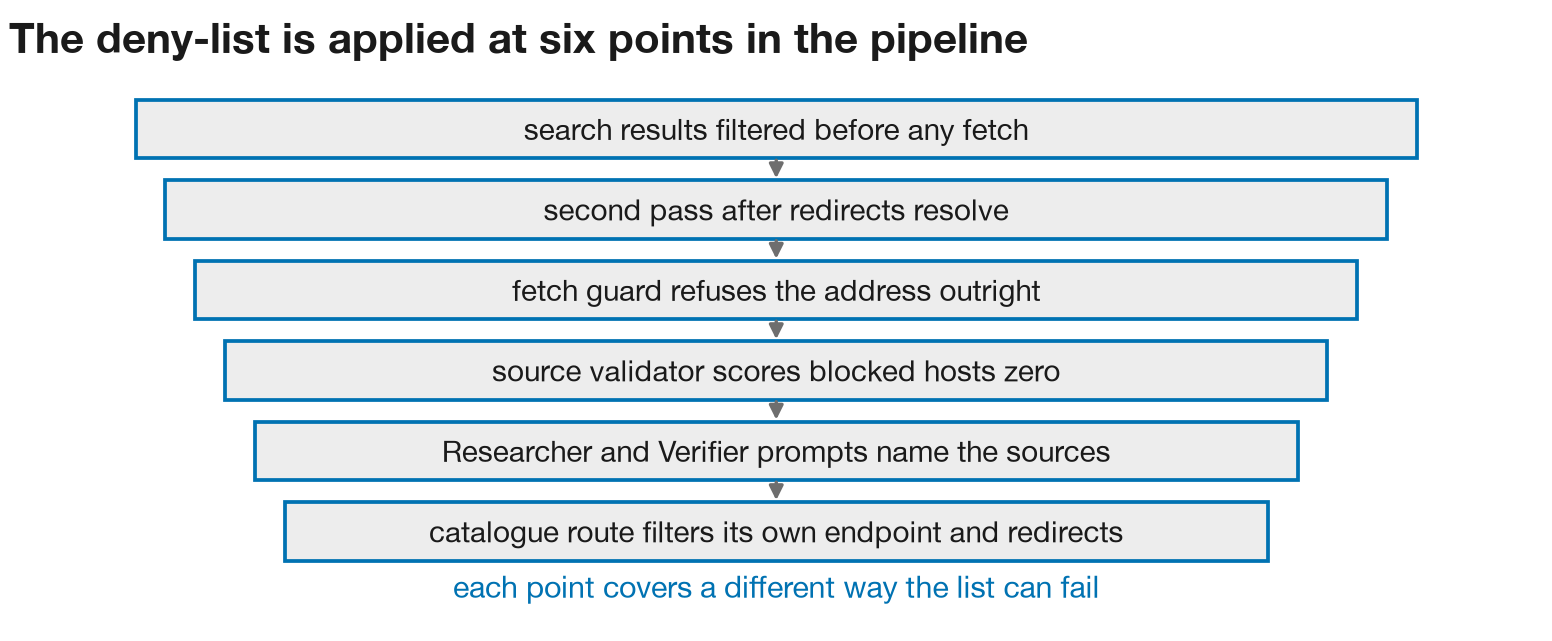
\includegraphics[width=7.08611in,height=2.92222in]{media/media/image7.png}

Figure 3.2: The six points at which the deny-list is applied.

Six points in the pipeline apply the deny-list, and Figure 3.2 sets out how each covers a different way it can fail. The search stage removes blocked results before they are fetched, and a second pass checks the set again afterwards in case a redirect has led somewhere blocked. The fetch guard refuses the address before any request is sent, and records the refusal against that question. The source validator gives blocked domains a trust score of zero, which stops them being used as evidence. The Researcher and Verifier prompts both name the forbidden sources and tell the agents not to use them. The deterministic catalogue route applies the same list to its own endpoint and to every redirect it follows.

Prior knowledge escapes retrieval controls entirely, since a model trained on text containing the published answers could reproduce them without issuing a query. The 2025 ODMI report was published on 19 December 2025, within the January 2026 training-data window of Sonnet 4.6. A closed-book probe bounds it empirically by repeating an evaluation with retrieval disabled, and the resulting accuracy is compared against the score a system would reach by answering ``yes'' to every binary question, 59.4\% on these eight countries. A model reciting a memorised key would beat that baseline; a model without one would not. Republication of the answer key on a permitted domain remains uncontrolled, since a consultancy write-up or news summary can restate a country\textquotesingle s answers without a listed host or fragment, and content-level fingerprinting of the published answers has not been built.

\section{Evaluation Set}\label{evaluation-set}

All tuning ran on a development set of five countries. The Netherlands and Malta served as balanced cases no-share, the proportion of a country\textquotesingle s binary questions whose published answer is ``no'', at 22\% and 31\%, Albania at 23\% with a low-resource language and a small open-data estate, and Norway and France as near-uniform yes cases at 8\% and 1\%. The 156-pair tuning battery ran on Malta, the Netherlands and Albania, picking out all their no golds and an equal number of randomly chosen yes gold questions. The threshold sweeps, the choice of retrieval pipeline, the search scope, the snippet cap and the ablations in §4.7 were all run on this set, leaving the evaluation countries untouched by tuning. The full list of experiments run for both tuning and results is detailed in Appendix C.

A system carrying an unchecked optimism bias scores well simply by answering ``yes'', and it scores best against the countries that answer ``yes'' most. A false-positive rate can only be measured where the key says ``no'', and those answers concentrate in the low-maturity tail, falling from 85\% of Bosnia's binary questions to none of Lithuania's. Discrimination is therefore only observable at the low-maturity end of the range, among countries that also tend not to meet many of the requirements a high-quality portal is scored on. The evaluation set therefore oversamples countries where negative golds are dense, since a random sample would be dominated by all-yes responses and the false-positive rate would rest on too few items to interpret. A further consequence is that countries are less likely to publish evidence that their open data falls short than evidence that it complies, so lower-maturity countries are expected to abstain more often.

Throughout development, eight countries were held out from all tuning to form the evaluation set, chosen on language resource level and overall no-share. Resource level is taken from the six-class taxonomy of Joshi et al. (2020), which grades a language from 0 to 5 on the labelled and unlabelled data available for it. Stratum A takes the four highest no-share countries outside the development set whose main language sits at class 3 or below, which gives Bosnia and Herzegovina, North Macedonia, Montenegro and Bulgaria. Stratum B takes the four highest at class 4 or above, giving Finland, Croatia, Sweden and Belgium. Figure 3.3 places each country at its class. Montenegrin is not listed, but it is a variety of the same South Slavic language as Bosnian, so it is read here as class 3. Between them the eight carry 1,144 question-country pairs and 368 binary negative golds, 261 of which sit in stratum A. The taxonomy predates the current generation of multilingual models and records catalogued resource counts rather than measured comprehension.

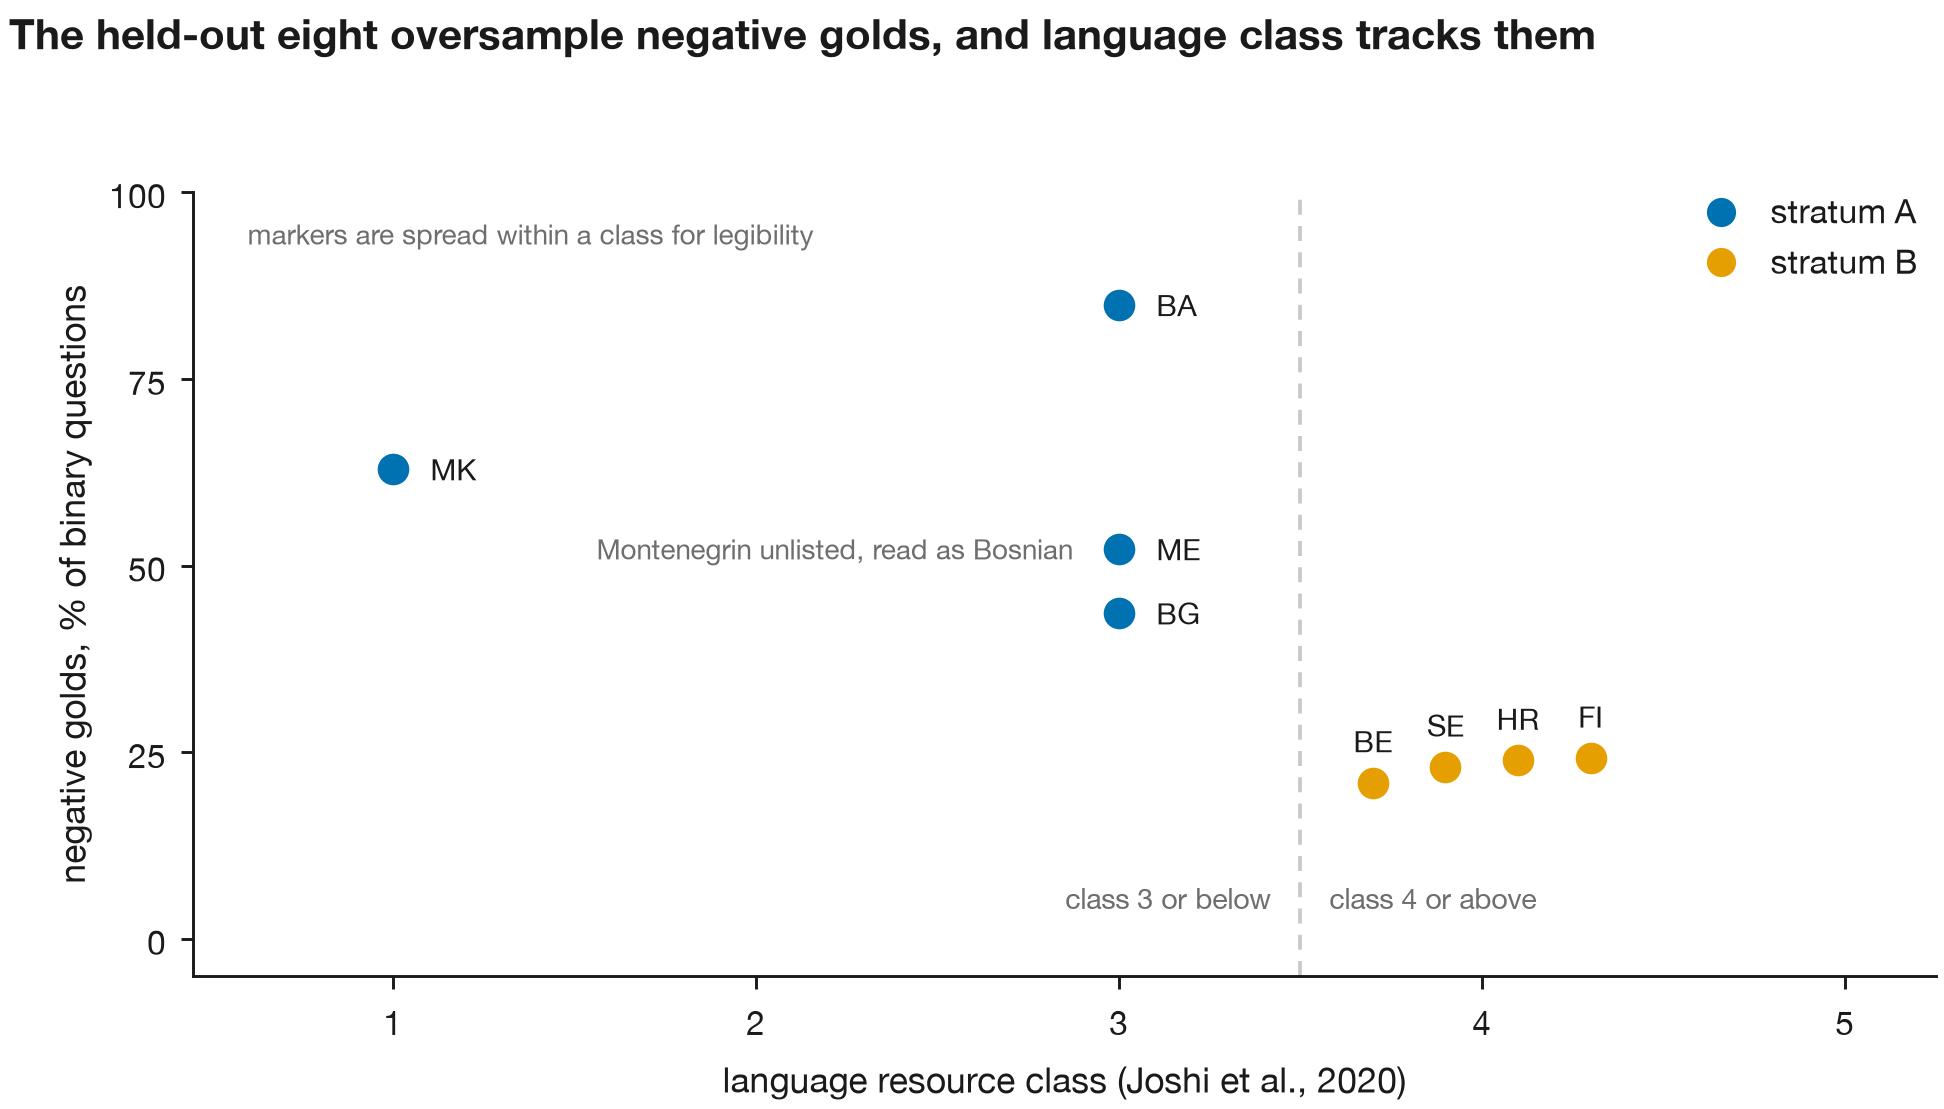
\includegraphics[width=7.08611in,height=4.03889in]{media/media/image8.png}

Figure 3.3: The evaluation eight by language resource class and negative-gold share.

§2.7 outlines three reasons a country might score poorly: the model misreads native-language evidence, the evidence is absent from the web, or the country is less open. The strata address the first reason. A markedly higher false-positive rate in stratum A would show that weaker comprehension of a national language makes the system commit wrong answers rather than making it decline. Conversely, a stable rate across strata indicates that success depends more on evidence retrieval. The strata are not matched for maturity, as Figure 3.3 shows. Stratum A ranges from 43.6\% `no-share' in Bulgaria to 84.8\% in Bosnia, while stratum B spans 20.9\% in Belgium to 24.2\% in Finland. Thus language class and maturity co-vary, and a result in stratum A bounds the language effect instead of isolating it.

\section{Experiments}\label{experiments}

The experimental programme divides into two classes, those used to tune the system in development, and those used to derive the results in §4. The tuning experiments settle design questions inside the system, for example, whether the Verifier issues its own counter-search, how many results each query returns, how broadly each query searches, and which variant of the Researcher prompt is used. All of these run on the development countries, and each is dispatched with an adoption rule written in advance, stating what result would displace the incumbent setting and by what margin. The results experiment is a single run of one frozen configuration of the architecture across the eight evaluation countries, which are not touched during any tuning experiment.

Every experiment is registered before dispatch, in a design note fixing the question, the sample, the endpoint and the adoption rule, and in a machine-readable row recording the same design. The orchestrator refuses to start a run that breaks any of five conditions, listed in Appendix C, and each is a hard failure that halts the run before any expenditure. The two that bear on the results are that no specification may name an evaluation country, and that experiments varying retrieval or measuring cost are forced onto a cold cache, since the search cache is keyed on the query and two arms sharing a warm cache would read one another's evidence. A single declared exception exists for the full results run, which must contain no development country.

Many experiments found no improvement on the incumbent design, particularly on the reasoning side. Where an arm did not clear its rule, the incumbent setting was retained and the null result was recorded in the same way as any other outcome.

The completed experiments are set out in §8.3, together with the question each addresses, its sample, its arms and its adoption rule.

The analysis that produces the figures reported in §4 is itself under test, as are the constraints above, which fail visibly if they are removed.

\section{Metrics}\label{metrics}

The following metrics, set out in Table 3.3, will be used in §4 to evaluate the results.

Table 3.3: Metrics reported in §4.

{\def\LTcaptype{none} % do not increment counter
\begin{longtable}[]{@{}
  >{\raggedright\arraybackslash}p{(\linewidth - 4\tabcolsep) * \real{0.2451}}
  >{\raggedright\arraybackslash}p{(\linewidth - 4\tabcolsep) * \real{0.5196}}
  >{\raggedright\arraybackslash}p{(\linewidth - 4\tabcolsep) * \real{0.2353}}@{}}
\toprule\noalign{}
\begin{minipage}[b]{\linewidth}\raggedright
\textbf{Metric}
\end{minipage} & \begin{minipage}[b]{\linewidth}\raggedright
\textbf{What it measures}
\end{minipage} & \begin{minipage}[b]{\linewidth}\raggedright
\textbf{Denominator}
\end{minipage} \\
\midrule\noalign{}
\endhead
\bottomrule\noalign{}
\endlastfoot
Coverage & Share of attempted pairs the system commits to. The complement of the abstention rate & All attempted pairs \\
Commit-accuracy & Share of committed answers matching the key & Scorable committed pairs \\
Per-class recall & Share of one gold class answered correctly, reported separately for yes and no golds & All golds in the class, and committed golds alone \\
Negative-gold false-positive rate & Share of negative golds the system answered ``yes''. A negative gold is one whose key answer is no, or a low band & All negative golds, and committed negative golds alone \\
Balanced accuracy & Mean of the true-positive and true-negative rates, removing the class imbalance that raw accuracy rewards. 0.5 is the floor, and below it the system is doing worse than answering the same way every time & Binary gold pairs \\
Expected calibration error & Mean gap between stated confidence and observed accuracy, weighted by bin size. Zero is perfect & Committed answers, binned by stated confidence \\
Selective risk & Accuracy against surviving coverage as the commit threshold sweeps upward & Pairs surviving at each threshold \\
McNemar\textquotesingle s test & Whether two systems differ, using only the items on which they disagree. A small p is evidence of a real difference; a high p does not establish equivalence, only that this sample could not separate them & Discordant pairs \\
Wilson interval & 95\% interval on a proportion. Holds at small n and at rates near 0 or 1. Non-overlapping intervals separate two arms; overlapping ones need a paired test & The rate\textquotesingle s own n \\
Spearman\textquotesingle s rank correlation & Whether two orderings agree, on {[}-1, 1{]}, where +1 is the same order & The ranked items \\
\end{longtable}
}

An abstention is neither correct nor incorrect, so every rate over a gold class has two defensible denominators. Taken over committed answers alone, a rate scores only what the system said, which rewards declining whenever it is unsure. Taken over every gold in the class, an abstention counts as a failure, which rewards answering regardless. Neither denominator is honest by itself, so §4 reports both. Coverage is read beside every accuracy figure, since abstaining on all but one pair and getting it right returns a commit-accuracy of 100\%.

\chapter{Results}\label{ch:results}

Chapter~\ref{ch:methodology} laid out the architecture, the evaluation set and the evaluation metrics for measuring success. This chapter details the results of running a sample of eight countries. The first six sections test the swarm against the six criteria of Section~\ref{sec:criteria}. Section~\ref{sec:ablation} looks at the added value of each component in the swarm, and whether the stance of the Verifier is load-bearing. Section~\ref{sec:cost-runtime} discusses the timeliness and cost of running the swarm, and Section~\ref{sec:reconstruction} turns the view onto the ODMI itself, reconstructing the maturity score the assessment would publish and asking what work would be left to the people overseeing it.

One finding runs through the chapter. The swarm can evidence a ``yes'' by finding a document and quoting the line. A ``no'' usually rests on not finding one, and an absence cannot be quoted, so the swarm commits its negative answers at the bottom of the confidence scale and abstains on many it would have got right. Each section below runs into it again. Adding agents to the loop raises the share of questions answered from 26.6\% to 55.6\% and the number of correct answers from 220 to 437, as Section~\ref{sec:ablation} sets out, while commit accuracy falls from 74.3\% to 70.1\%. Swapping the Verifier from an adversarial stance to a corroborative one leaves accuracy where it was, and the corroborative arm commits more false positives on the negative golds, 27.2\% against 23.4\%, though the difference is not significant. Abstention falls unevenly across the two answer classes. The confidence score rates how well the retrieved evidence supports a claim, and an absence gives it nothing to weigh, so an answer of ``no'' scores low however sound it is. Of the 88 withheld answers sitting below the floor on a negative gold, 73 were correct. What limits the system is that the open web rarely publishes evidence that a practice is absent.

\section{Convergent Validity}\label{sec:convergent-validity}



\begin{figure}[htbp]
\centering
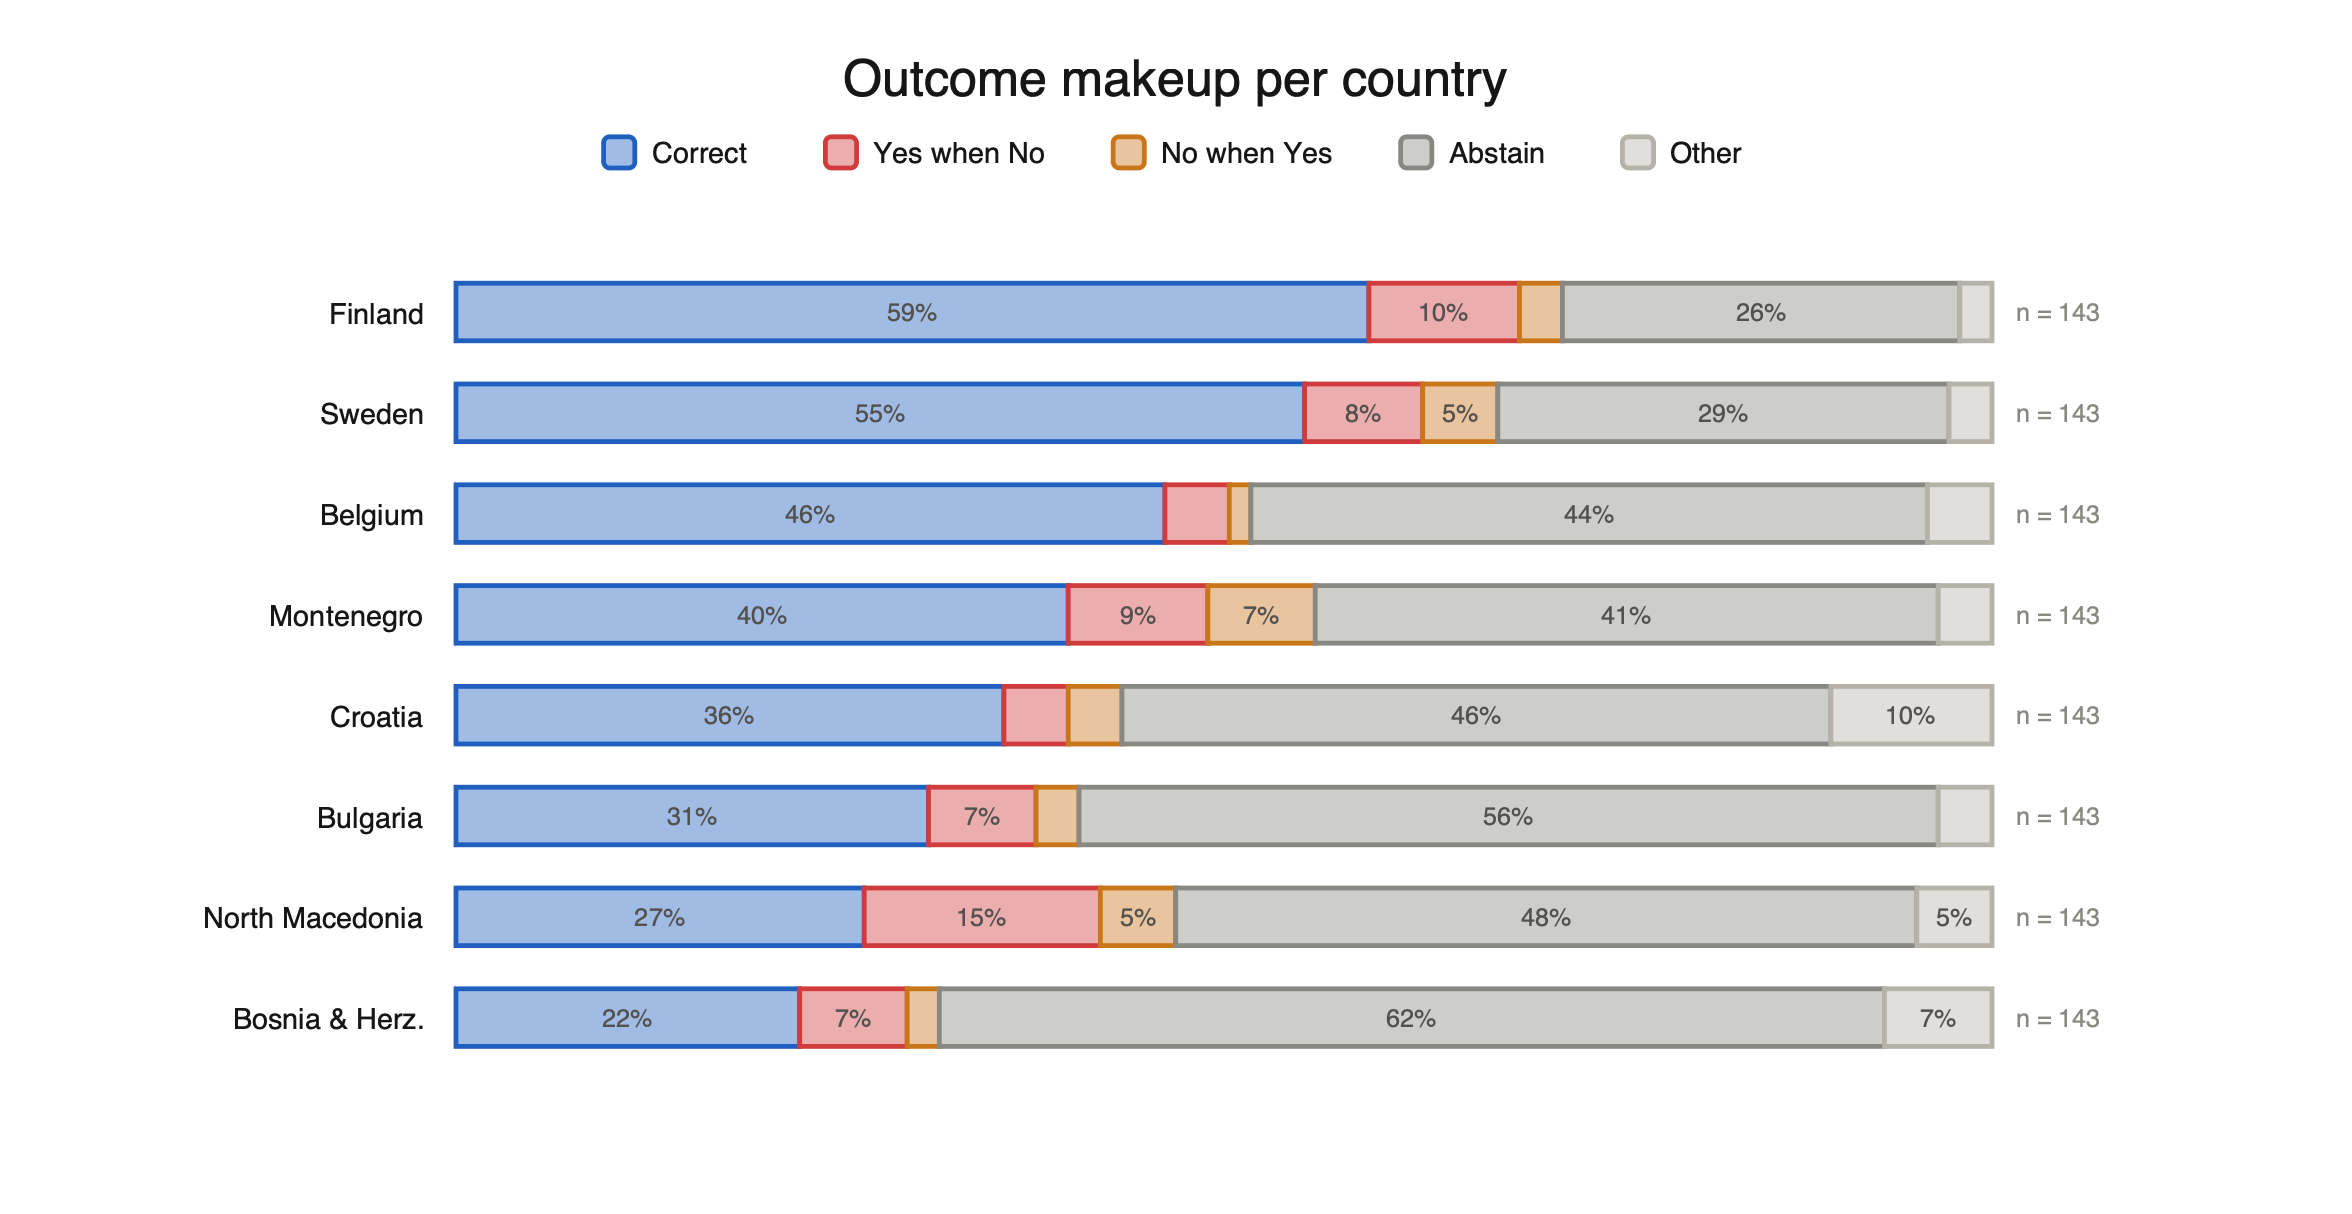
\includegraphics[width=\linewidth]{figures/outcome_makeup_per_country.png}
\caption{Outcome make-up per country.}
\label{fig:outcome-makeup}
\end{figure}

\begin{longtable}[]{@{}
  >{\raggedright\arraybackslash}p{(\linewidth - 10\tabcolsep) * \real{0.2549}}
  >{\raggedright\arraybackslash}p{(\linewidth - 10\tabcolsep) * \real{0.1471}}
  >{\raggedright\arraybackslash}p{(\linewidth - 10\tabcolsep) * \real{0.1471}}
  >{\raggedright\arraybackslash}p{(\linewidth - 10\tabcolsep) * \real{0.1471}}
  >{\raggedright\arraybackslash}p{(\linewidth - 10\tabcolsep) * \real{0.1471}}
  >{\raggedright\arraybackslash}p{(\linewidth - 10\tabcolsep) * \real{0.1569}}@{}}
\caption{The evaluation run read four ways. Coverage is over all 1,144 pairs. The accuracy columns are over the 907 whose published answer is a plain yes or no. Every rate carries its own denominator, and the forced and closed-book rows score an abstention as a miss.}\label{tab:four-ways}\\
\toprule\noalign{}
\begin{minipage}[b]{\linewidth}\raggedright
\textbf{Reading}
\end{minipage} & \begin{minipage}[b]{\linewidth}\raggedright
\textbf{Coverage}
\end{minipage} & \begin{minipage}[b]{\linewidth}\raggedright
\textbf{Accuracy}
\end{minipage} & \begin{minipage}[b]{\linewidth}\raggedright
\textbf{Yes golds}
\end{minipage} & \begin{minipage}[b]{\linewidth}\raggedright
\textbf{No golds}
\end{minipage} & \begin{minipage}[b]{\linewidth}\raggedright
\textbf{Balanced}
\end{minipage} \\
\midrule\noalign{}
\endfirsthead
\toprule\noalign{}
\begin{minipage}[b]{\linewidth}\raggedright
\textbf{Reading}
\end{minipage} & \begin{minipage}[b]{\linewidth}\raggedright
\textbf{Coverage}
\end{minipage} & \begin{minipage}[b]{\linewidth}\raggedright
\textbf{Accuracy}
\end{minipage} & \begin{minipage}[b]{\linewidth}\raggedright
\textbf{Yes golds}
\end{minipage} & \begin{minipage}[b]{\linewidth}\raggedright
\textbf{No golds}
\end{minipage} & \begin{minipage}[b]{\linewidth}\raggedright
\textbf{Balanced}
\end{minipage} \\
\midrule\noalign{}
\endhead
\bottomrule\noalign{}
\endlastfoot
Aggregate Accuracy & 100\% & \begin{minipage}[t]{\linewidth}\raggedright
42.4\%\\
385/907\strut
\end{minipage} & \begin{minipage}[t]{\linewidth}\raggedright
54.7\%\\
295/539\strut
\end{minipage} & \begin{minipage}[t]{\linewidth}\raggedright
24.5\%\\
90/368\strut
\end{minipage} & 39.6\% \\
Commit Accuracy & \begin{minipage}[t]{\linewidth}\raggedright
55.6\%\\
636/1,144\strut
\end{minipage} & \begin{minipage}[t]{\linewidth}\raggedright
70.1\%\\
437/623\strut
\end{minipage} & \begin{minipage}[t]{\linewidth}\raggedright
87.0\%\\
295/339\strut
\end{minipage} & \begin{minipage}[t]{\linewidth}\raggedright
48.9\%\\
90/184\strut
\end{minipage} & 68.0\% \\
Closed book, retrieval off & 75.6\%865/1,144 & \begin{minipage}[t]{\linewidth}\raggedright
43.0\%\\
390/907\strut
\end{minipage} & \begin{minipage}[t]{\linewidth}\raggedright
43.6\%\\
235/539\strut
\end{minipage} & \begin{minipage}[t]{\linewidth}\raggedright
42.1\%\\
155/368\strut
\end{minipage} & 42.9\% \\
Always-yes baseline & 100\% & \begin{minipage}[t]{\linewidth}\raggedright
59.4\%\\
539/907\strut
\end{minipage} & 100\% & 0\% & 50.0\% \\
\end{longtable}

The swarm was dispatched over all 1,144 question-country pairs of the eight countries. It committed to an answer on 636 and declined the remaining 508, split by country in Figure~\ref{fig:outcome-makeup}, a coverage of 55.6\%. Over just the committed answers it scored an accuracy of 70.1\%. Table~\ref{tab:four-ways} presents the results, distinguishing aggregate accuracy (including abstentions), commit accuracy (excluding abstentions), the accuracy of always answering ``yes'', and the accuracy of using only the model's priors. The table compares the 907 pairs that take a binary answer and carry a plain yes or no in the key. The remaining 237 either ask for a band or a count, where an always-yes baseline has no meaning, or are questions the assessors did not answer ``yes'' or ``no''.


Scoring every abstention as an error gives a strict lower bound. On that reading the swarm reaches 42.4\% accuracy, against the 59.4\% returned by arbitrarily answering ``yes'' to every question. Balanced accuracy, the mean of the yes- and no-recalls, falls to 39.6\%, against the 50.0\% any single-class rule achieves by construction. This reading is not how the system was intended, as many questions do not have sufficient public evidence to answer, and thus abstention is the correct path in these cases, but it establishes that the system has no aggregate advantage over the majority class once abstention is removed.

Section~\ref{sec:llm-limitations} raised the issue of generative models using prior beliefs to steer their information retrieval, and a closed-book run over the same eight countries, with retrieval disabled so that the model answers from its parameters alone, reaches 43.0\% on the same 907 golds. Aggregate accuracy and closed book accuracy are indistinguishable. Retrieval therefore buys no measurable gain once every abstention is counted as a wrong answer. The difference appears in the two classes. Without retrieval the model is close to symmetric, recovering 43.6\% of yes golds and 42.1\% of no golds. With retrieval the swarm recovers 87.0\% and 48.9\%. What the pipeline finds settles a positive claim and does little for a negative one, which is the asymmetry Section~\ref{sec:llm-limitations} predicted and the remainder of this chapter returns to.



\begin{figure}[htbp]
\centering
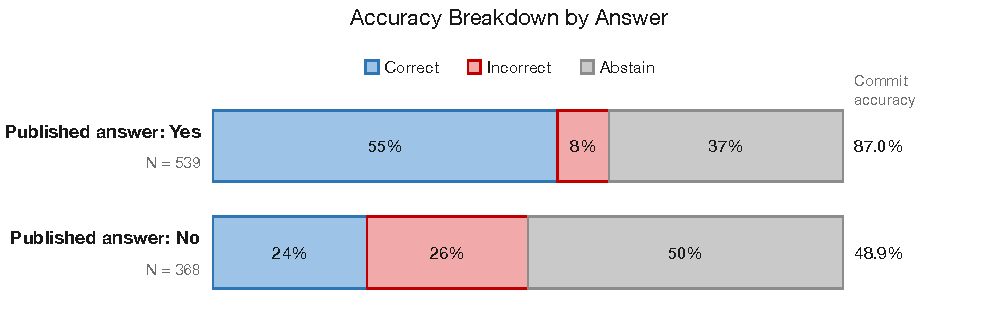
\includegraphics[width=\linewidth]{figures/fig_4_1_yes_no.pdf}
\caption{Decomposition of accuracy by answer class.}
\label{fig:accuracy-by-class}
\end{figure}

Accuracy divides unevenly between the two answer classes. Where the published key records a ``yes'', the swarm committed on 339 of 539 pairs and agreed with the key on 87.0\% of them. Where the key records a ``no'', it committed on 184 of 368 and agreed on 48.9\%, so on the negative golds it commits to, it is wrong more often than right. Abstention divides the same way, as Figure~\ref{fig:accuracy-by-class} shows. The swarm declines exactly half the negative golds against 37.1\% of the positive ones. The answer it withholds most often is the one that records a country falling short.

The error the Verifier exists to prevent is a committed ``yes'' against a negative gold. The run contains 91 of them, 24.7\% of all 368 negative golds and 49.5\% of the 184 the swarm was willing to commit on. Offered the choice between declining and asserting a ``yes'' the evidence does not carry, it asserts about half the time.

On the first condition of Convergent Validity the system reaches 70.1\% commit accuracy at 55.6\% coverage. It agrees with the existing process on most of the answers it gives, and it gives an answer to just over half the questions.



\begin{figure}[htbp]
\centering
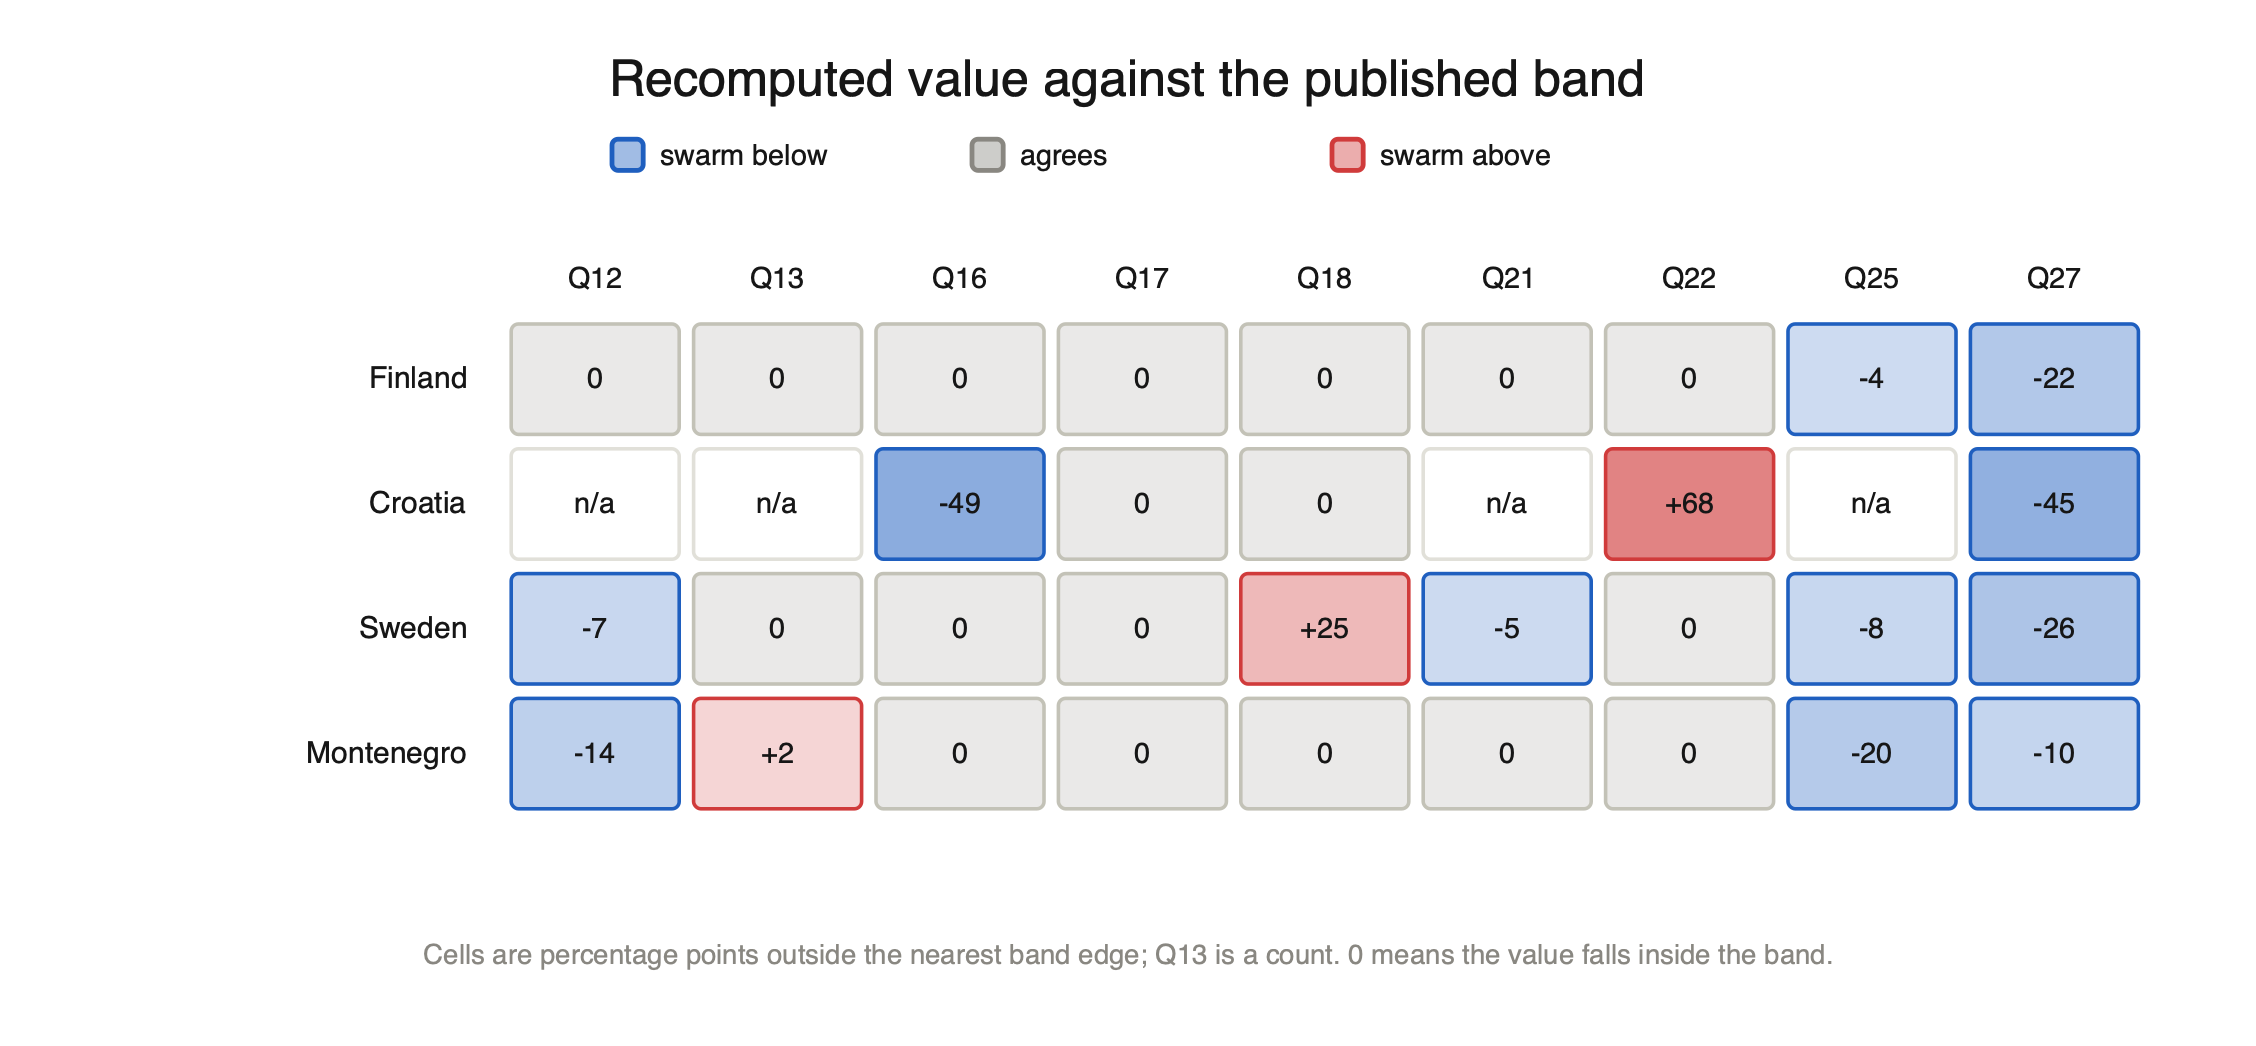
\includegraphics[width=\linewidth]{figures/recompute_vs_band.png}
\caption{Recomputed value against the published band.}
\label{fig:recompute-band}
\end{figure}

Only four of the eight countries (Finland, Croatia, Sweden and Montenegro) had harvestable portals.

Across the thirty-six measurable cells the recompute agrees with the published key on eighteen, 50\% agreement, broken down by country in Figure~\ref{fig:recompute-band}. The disagreements do not all run in the same direction, so this is not a case of countries systematically inflating their score. The figure shows the numbers diverging, with Montenegro\textquotesingle s stated licence coverage exceeding 90\% where the recompute reads 70\%, an overstatement, while Croatia\textquotesingle s published figure for Q22 sits at 10-30\% against a recompute above 90\%, an understatement of what the portal actually carries. This recompute is not infallible, as the Verifier recomputes the scores over the cached data that the Researcher retrieved, and there is no separate route or evidence pool to check against.

Convergent Validity is therefore only half met. The system reproduces the existing process on 70.1\% of the answers it commits to. The recompute tested the harder question, whether the figures a country reports about its own portal survive a check against the portal itself. On these nine they do not. The self-report and an independent count disagree on 50\% of the measurable cells, which is evidence that the reported figures on the objective quality questions are often inaccurate. It falls short of proof, because the recompute has no route independent of the Researcher\textquotesingle s harvest, so no single figure is settled. Capgemini already amends 10\% of the answers countries submit, which is the assessment\textquotesingle s own admission that self-reports are sometimes wrong, and on the small set of questions where an outside check is possible, the recompute points the same ways.

\section{Selectivity}\label{sec:selectivity}

Abstention exists so the swarm does not commit answers with shaky underlying evidence. Table~\ref{tab:abstention-reasons} breaks the 508 abstentions down by reason, and Appendix~\ref{app:pipeline-detail} carries the full trail. Every one passed through the Adjudicator, which returned an abstain verdict on 413; a commit gate withheld a further 82 at the 0.65 floor, and in 13 more the Adjudicator's own answer was inconclusive. No abstention in this run came from an empty search, and a gold answer existed for 94.3\% of these questions.

\begin{longtable}[]{@{}
  >{\raggedright\arraybackslash}p{(\linewidth - 4\tabcolsep) * \real{0.4531}}
  >{\raggedright\arraybackslash}p{(\linewidth - 4\tabcolsep) * \real{0.2031}}
  >{\raggedright\arraybackslash}p{(\linewidth - 4\tabcolsep) * \real{0.3437}}@{}}
\caption{Why the swarm abstained.}\label{tab:abstention-reasons}\\
\toprule\noalign{}
\begin{minipage}[b]{\linewidth}\raggedright
\textbf{Reason for abstaining}
\end{minipage} & \begin{minipage}[b]{\linewidth}\raggedright
\textbf{Pairs}
\end{minipage} & \begin{minipage}[b]{\linewidth}\raggedright
\textbf{Share of abstentions}
\end{minipage} \\
\midrule\noalign{}
\endfirsthead
\toprule\noalign{}
\begin{minipage}[b]{\linewidth}\raggedright
\textbf{Reason for abstaining}
\end{minipage} & \begin{minipage}[b]{\linewidth}\raggedright
\textbf{Pairs}
\end{minipage} & \begin{minipage}[b]{\linewidth}\raggedright
\textbf{Share of abstentions}
\end{minipage} \\
\midrule\noalign{}
\endhead
\bottomrule\noalign{}
\endlastfoot
Verifier rejected the evidence & 208 & 40.9\% \\
Researcher never reached the floor & 199 & 39.2\% \\
Researcher never committed & 30 & 5.9\% \\
Quote absent from retrieved pages & 24 & 4.7\% \\
Instrumentation mismatch & 19 & 3.7\% \\
Fetch error & 16 & 3.1\% \\
Blocked by the deny-list & 12 & 2.4\% \\
All abstentions & 508 & 100.0\% \\
\end{longtable}


Section~\ref{sec:open-world} highlighted how moving the evidence pool from self-reporting to the open web means absence of evidence of a practice no longer equates to absence of the practice itself. Question PT28 asks, ``Do you monitor search key words?''. It is easier to find evidence when the national data team do follow a practice, since they may have posted on their portal that they do. For the swarm to mark it ``no'' with confidence, it must find concrete evidence that they do not, and a national data team is unlikely to publish that it is not following a practice. Accordingly, 19 of the 143 questions were abstained on by at least 7 countries, and 12 of these covered internal practices. Any evidence the swarm finds may be related to the practice without directly addressing it, so it will be less confident in these answers. This is reflected in the results: across all answer shapes the swarm abstains on 50.0\% of no golds against 37.1\% of yes golds.

Figure~\ref{fig:per-class-confidence} sweeps the confidence threshold required to commit an answer from 0.40 upwards and rescores the gold classes on what survives at each setting. The two classes diverge as the threshold increases. On yes golds the threshold acts as expected, with accuracy climbing from 87.0\% at the 0.65 floor and reaching 100\% near 0.95, on nine answers. On no golds it moves the other way, falling from 48.9\% at the floor to zero by about 0.81 and staying there.\textbf{ }



\begin{figure}[htbp]
\centering
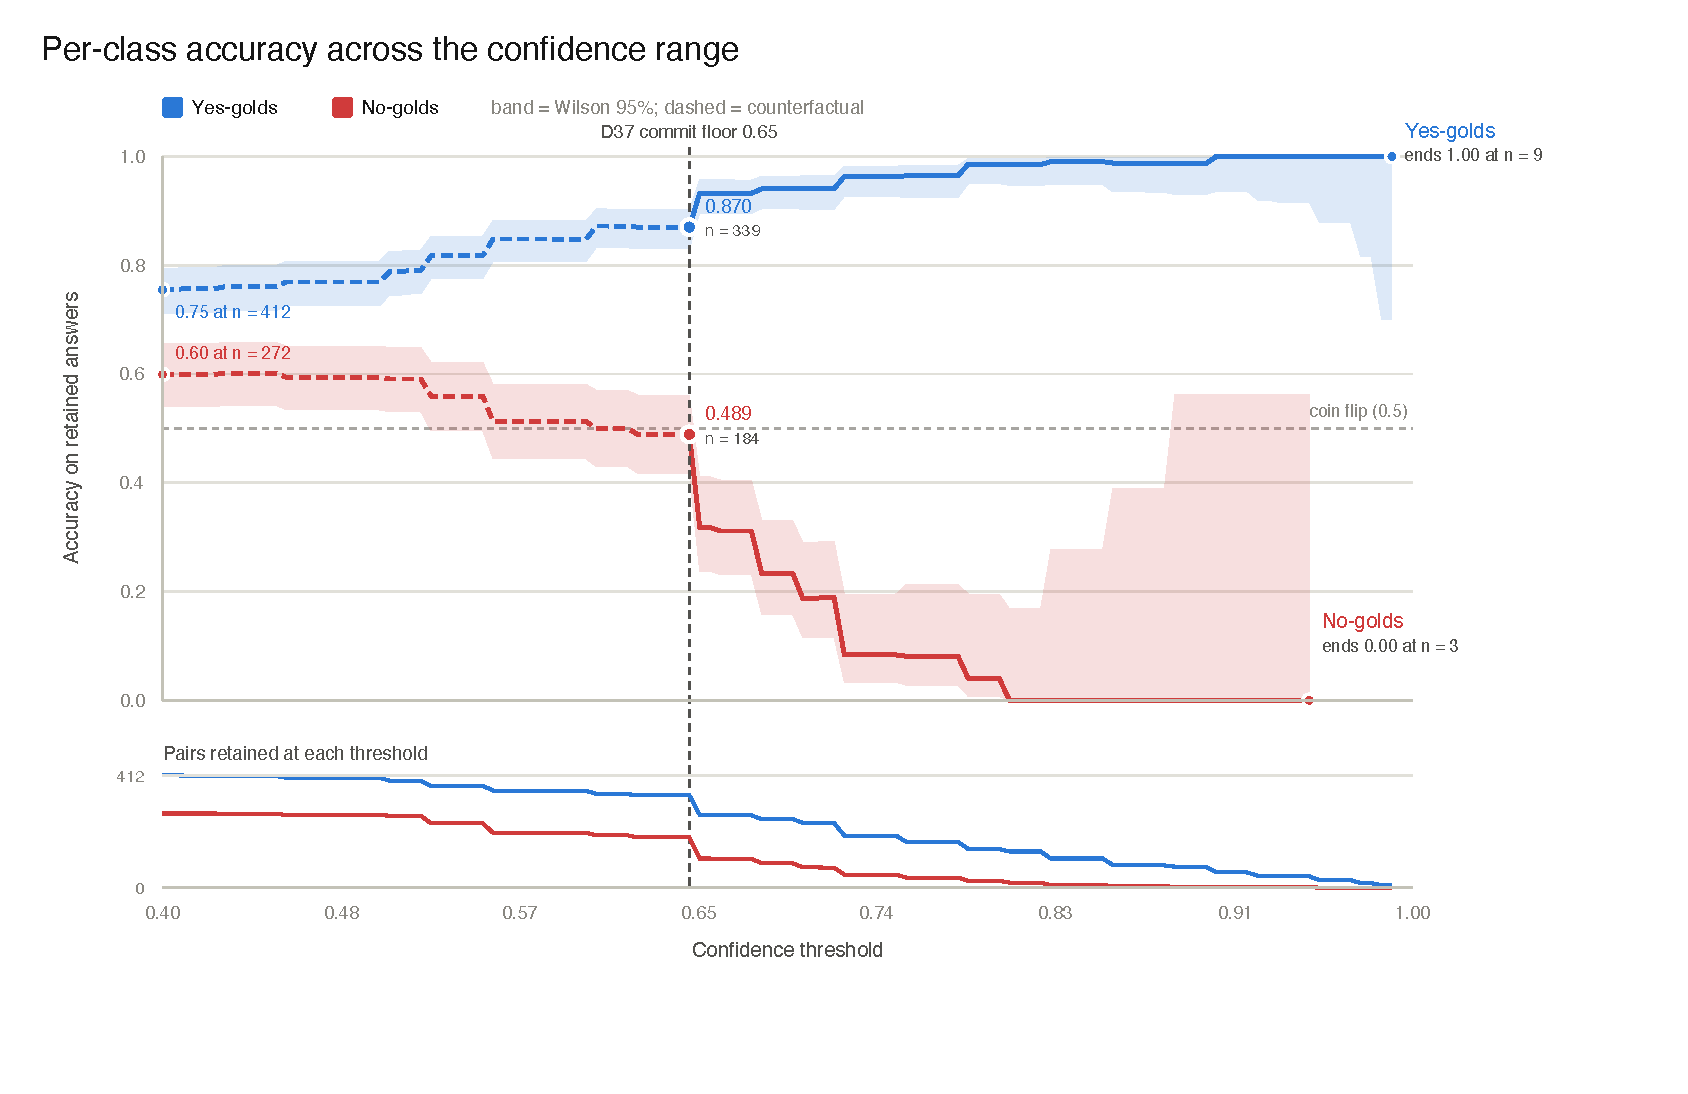
\includegraphics[width=\linewidth]{figures/per_class_accuracy_full_range.pdf}
\caption{Per-class accuracy across the confidence range.}
\label{fig:per-class-confidence}
\end{figure}

Calibration shows the same inversion. A stated confidence of 0.8 should correspond to being right about 80\% of the time. Across all 623 scoreable committed answers the expected calibration error is 0.063, which taken alone reads as a well-calibrated system. Figure~\ref{fig:reliability} shows otherwise. On the yes golds every point sits on or above the diagonal, so the system is modestly under-confident, which is a more harmless direction in which to err. On the no golds the sequence runs backwards and the expected calibration error is 0.299, nearly five times the aggregate. The aggregate conceals this because the classes are unevenly spread across the range, with only 3 negative samples in the uppermost bin against 77 yes golds. Because nothing commits below 0.65, six of the ten pre-registered bins are empty and calibration is observable only across the upper third of the scale.



\begin{figure}[htbp]
\centering
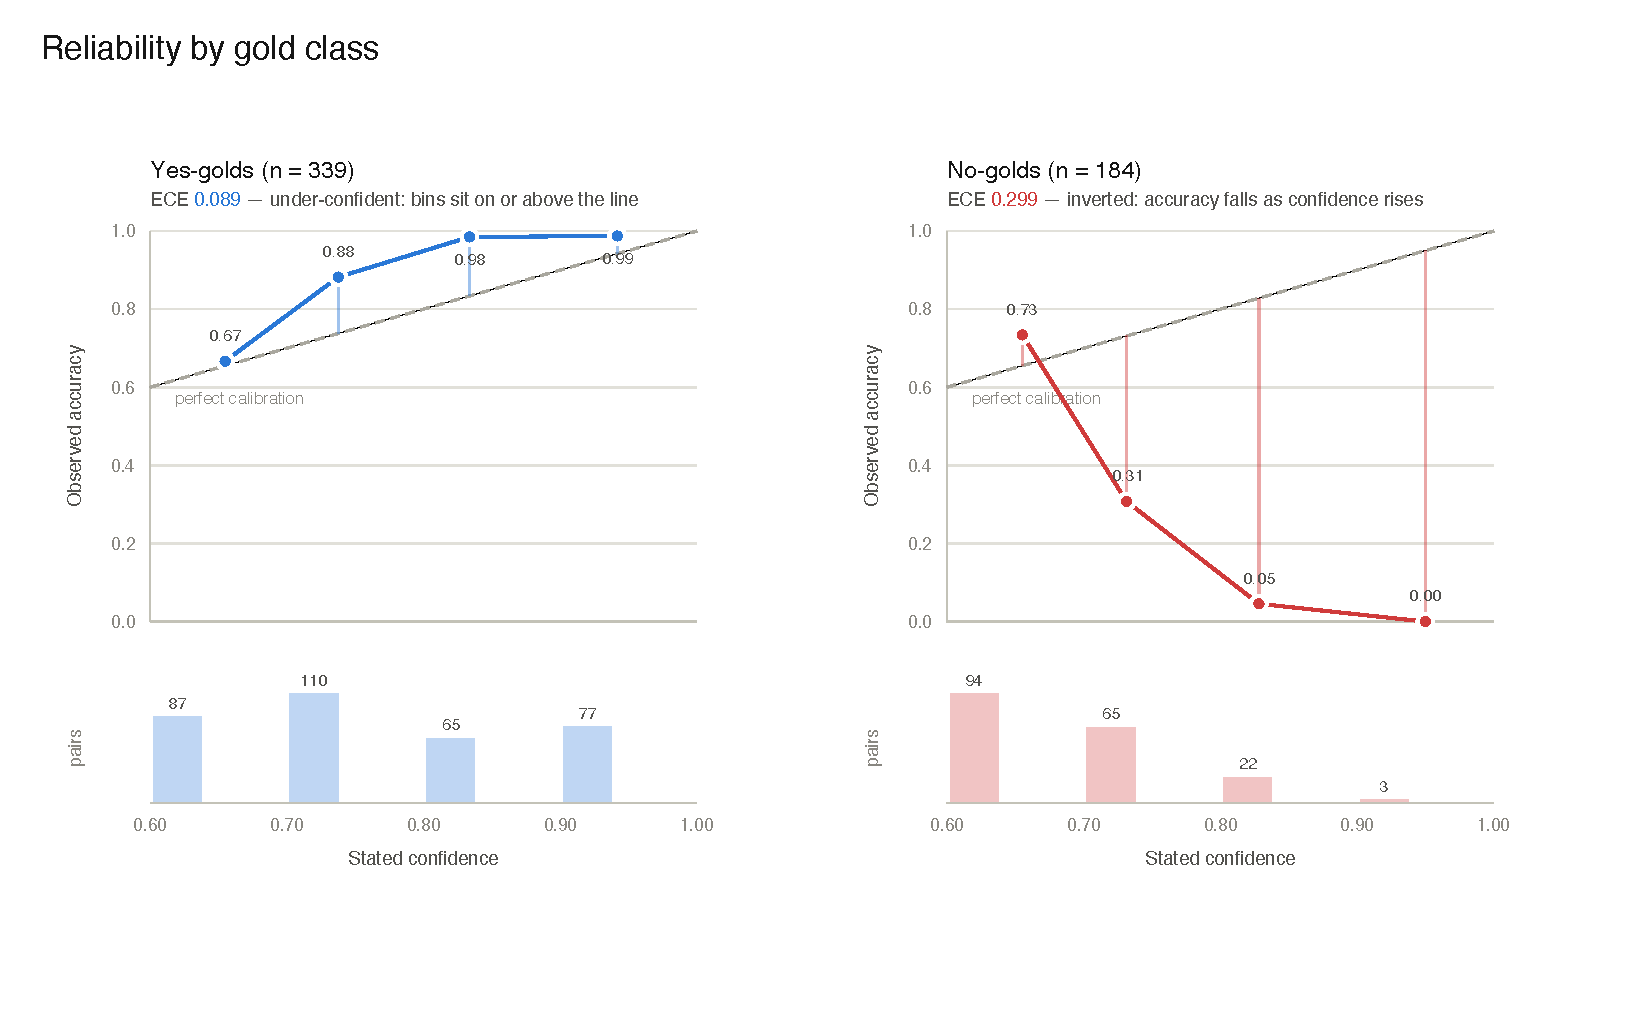
\includegraphics[width=\linewidth]{figures/reliability_by_class.pdf}
\caption{Reliability by gold class.}
\label{fig:reliability}
\end{figure}

The inversion continues below the floor. The dashed segment of Figure~\ref{fig:per-class-confidence} scores answers the swarm produced and then withheld, all from pairs where the Researcher never reached 0.65 on any attempt. Of the 162 that are scoreable, 73 carry a yes gold and 89 carry a no gold. Around a quarter of the yes answers are correct, against 79 of the 89 no answers. The negatives the system is least sure of are the ones it gets right, and the same holds just above the floor, where the 0.65 to 0.70 group is correct 73\% of the time. When the swarm cannot find evidence for a question, which is what would constitute a ``no'' under a closed-world assumption, it outputs a low confidence score because any evidence it did retrieve was weak. The information is therefore present in the score and cannot be used, because these correct ``noes'' look the same as the incorrect ``yesses'', so there can be no separation before looking at the key. There are also far more ``yesses'' than ``noes'' in the answer key, so optimising the threshold on raw accuracy would favour maximising the chance of getting a ``yes'' correct, losing many correct ``noes'' with them.

Selectivity as implemented meets the first of Section~\ref{sec:criteria}'s two requirements and fails the second. The system does decline, on 44\% of pairs. The confidence attached to an answer measures how strongly the retrieved passage supports it, not how likely it is to be right, and thus negative golds, which hold little public evidence, frequently fall below the confidence floor. The system is well-calibrated for answering ``yes'', but systemically disadvantaged for answering ``no''.

\section{Attributability}\label{sec:attributability}

Attributability was defined in Section~\ref{sec:criteria} by two conditions. The quoted passage must exist in the source, and a reasonable reader must agree it supports the claim. The first is a string comparison the system enforces on every answer before it commits; the second needs a reader, and Section~\ref{sec:agent-loop} puts the Verifier in charge of this role. Attributability's value is that an assessed country knows its score rests on well-evidenced grounds, and can contest the evidence held against it.

The first condition is enforced mechanically. The offline gate described in Section~\ref{sec:agent-loop} compares the Researcher\textquotesingle s quoted passage against the snippets it read and fails the answer where the passage does not appear. It sits upstream of the commit decision, so all 636 committed answers passed it, and 24 of the run\textquotesingle s 508 abstentions record an ungrounded passage as the reason. Fabrication, one of the central risks of a generative assessor identified in Section~\ref{sec:llm-limitations}, is caught by a string comparison and is not what limits the system.

Testing for misinterpretation requires a `reasonable reader'. The Verifier\textquotesingle s role is to apply the scrutiny a human reader would bring to the submitted evidence. Table~\ref{tab:attributability} displays the 208 relevance rejections, which are pairs where the quote survived the string comparison and the Verifier ruled the evidence off-target anyway, so off-target evidence outnumbers absent evidence by more than eight to one.

\begin{longtable}[]{@{}
  >{\raggedright\arraybackslash}p{(\linewidth - 6\tabcolsep) * \real{0.3750}}
  >{\raggedright\arraybackslash}p{(\linewidth - 6\tabcolsep) * \real{0.3409}}
  >{\raggedright\arraybackslash}p{(\linewidth - 6\tabcolsep) * \real{0.1136}}
  >{\raggedright\arraybackslash}p{(\linewidth - 6\tabcolsep) * \real{0.1705}}@{}}
\caption{What each attributability condition caught, over the 1,144 evaluation pairs.}\label{tab:attributability}\\
\toprule\noalign{}
\begin{minipage}[b]{\linewidth}\raggedright
\textbf{Attributability condition}
\end{minipage} & \begin{minipage}[b]{\linewidth}\raggedright
\textbf{What fails it}
\end{minipage} & \begin{minipage}[b]{\linewidth}\raggedright
\textbf{Pairs}
\end{minipage} & \begin{minipage}[b]{\linewidth}\raggedright
\textbf{Share of 1,144}
\end{minipage} \\
\midrule\noalign{}
\endfirsthead
\toprule\noalign{}
\begin{minipage}[b]{\linewidth}\raggedright
\textbf{Attributability condition}
\end{minipage} & \begin{minipage}[b]{\linewidth}\raggedright
\textbf{What fails it}
\end{minipage} & \begin{minipage}[b]{\linewidth}\raggedright
\textbf{Pairs}
\end{minipage} & \begin{minipage}[b]{\linewidth}\raggedright
\textbf{Share of 1,144}
\end{minipage} \\
\midrule\noalign{}
\endhead
\bottomrule\noalign{}
\endlastfoot
The passage exists in the cited source & quote absent from the retrieved text & 24 & 2.1\% \\
A reader agrees it supports the claim & Verifier ruled the evidence off-target & 208 & 18.2\% \\
Both conditions cleared & answer committed & 636 & 55.6\% \\
Neither condition reached & abstained for another reason & 276 & 24.1\% \\
\end{longtable}


Scrutiny of the Researcher's claims from the Verifier raises the commit rate from 26.6\% to 46\% and the correct answers from 220 to 372 (Section~\ref{sec:ablation}). It converts 165 of the Researcher\textquotesingle s wrong or withheld answers into correct ones and loses 13 in the other direction, moving 178 answers in all. The Adjudicator improves upon this by committing an extra 110 answers and getting 65 right, and it overturns none of the Verifier\textquotesingle s existing decisions. This is the extent to which the architecture can ensure a `reasonable' reader is judging that claims are valid without an external model or human verification layer, and the Adjudicator correcting zero of the Verifier's claims hints that each reasoning stage converges closer to the true accuracy ceiling.

Opus 4.6 reviewed the 91 cases where the swarm committed a ``yes'' against a negative gold, with both the swarm\textquotesingle s evidence and the ODMI\textquotesingle s explanation in front of it, to test whether the swarm had misattributed its evidence or the published answer was wrong or out of date. On 84 of the 91 it judged the cited passage simply too weak to carry the claim. On the other seven it found the evidence sufficient and the published ``no'' defensible or out of date, and four of those seven carry no published explanation at all. Opus shares a training lineage with the Sonnet agents, so a stronger test is another model family or a human reader. What this small experiment confirmed is that misattribution is a failure mode of the swarm, rather than the answer key being consistently incorrect.

636 committed answers cleared the string comparison and 24 abstentions record a quote that did not, which settles the first condition. The Verifier performs the role of the reasonable reader well, halting 208 of the Researcher\textquotesingle s overreaching claims, but still lets through 91, showing the issue is not solved. In production, where there is no answer key to check against, the many overreads that slip through the system will remain undetected, and this is where an external model or human reviewer would be valuable.

\section{Subgroup Equity}\label{sec:subgroup-equity}

Subgroup Equity asks whether the same standard of assessment applied to every country. This section analyses which properties are incidental to maturity and which are inseparable from it, because only the first kind can be removed. The evaluation set was stratified to test the clearest incidental candidate, language comprehension. Section~\ref{sec:multilingual} set out three explanations for a poor score: the model misreads evidence written in the national language, the evidence is not published at all, or the country is truly less open. The two strata separate the first of these from the other two, with stratum A holding the four lower-resource languages (Bosnia and Herzegovina, North Macedonia, Montenegro and Bulgaria) and stratum B the four higher-resource ones (Finland, Croatia, Sweden and Belgium).

\begin{longtable}[]{@{}
  >{\raggedright\arraybackslash}p{(\linewidth - 10\tabcolsep) * \real{0.2059}}
  >{\raggedright\arraybackslash}p{(\linewidth - 10\tabcolsep) * \real{0.0882}}
  >{\raggedright\arraybackslash}p{(\linewidth - 10\tabcolsep) * \real{0.1275}}
  >{\raggedright\arraybackslash}p{(\linewidth - 10\tabcolsep) * \real{0.1863}}
  >{\raggedright\arraybackslash}p{(\linewidth - 10\tabcolsep) * \real{0.1863}}
  >{\raggedright\arraybackslash}p{(\linewidth - 10\tabcolsep) * \real{0.2059}}@{}}
\caption{Outcomes by resource stratum.}\label{tab:strata}\\
\toprule\noalign{}
\begin{minipage}[b]{\linewidth}\raggedright
\textbf{Stratum}
\end{minipage} & \begin{minipage}[b]{\linewidth}\raggedright
\textbf{Pairs}
\end{minipage} & \begin{minipage}[b]{\linewidth}\raggedright
\textbf{Abstention}
\end{minipage} & \begin{minipage}[b]{\linewidth}\raggedright
\textbf{Commit accuracy}
\end{minipage} & \begin{minipage}[b]{\linewidth}\raggedright
\textbf{Neg-gold FP (all)}
\end{minipage} & \begin{minipage}[b]{\linewidth}\raggedright
\textbf{Neg-gold FP (committed)}
\end{minipage} \\
\midrule\noalign{}
\endfirsthead
\toprule\noalign{}
\begin{minipage}[b]{\linewidth}\raggedright
\textbf{Stratum}
\end{minipage} & \begin{minipage}[b]{\linewidth}\raggedright
\textbf{Pairs}
\end{minipage} & \begin{minipage}[b]{\linewidth}\raggedright
\textbf{Abstention}
\end{minipage} & \begin{minipage}[b]{\linewidth}\raggedright
\textbf{Commit accuracy}
\end{minipage} & \begin{minipage}[b]{\linewidth}\raggedright
\textbf{Neg-gold FP (all)}
\end{minipage} & \begin{minipage}[b]{\linewidth}\raggedright
\textbf{Neg-gold FP (committed)}
\end{minipage} \\
\midrule\noalign{}
\endhead
\bottomrule\noalign{}
\endlastfoot
Stratum A (lower resource) & 572 & 52.3\% & 61.1\% (162/265) & 21.1\% (55/261) & 42.6\% (55/129) \\
Stratum B (higher) & 572 & 36.5\% & 76.8\% (275/358) & 33.6\% (36/107) & 65.5\% (36/55) \\
\end{longtable}


Stratum A has over double the negative-golds of B, and would be expected to perform worse as Section~\ref{sec:convergent-validity} found the swarm handles ``yesses'' far better than ``noes''. However, stratum A\textquotesingle s negative gold false positive rate is far lower than B\textquotesingle s in both aggregate and commit-only, at 0.211 against 0.336 in aggregate and 0.426 against 0.655 on committed negatives. The obvious objection is that stratum A simply declines more of the hard negatives. That does not hold, since the swarm abstains on 50.6\% of negative golds in stratum A against 48.6\% in stratum B. Weaker language comprehension did not produce confident error.

Table~\ref{tab:strata} shows that what rises in stratum A is abstention, at 52.3\% against stratum B\textquotesingle s 36.5\%, and commit accuracy is lower, at 61.1\% against 76.8\%. That appears to contradict the false-positive result, since a stratum with lower accuracy might be expected to make more of every kind of error. The two measures cover different populations. Commit accuracy covers every committed answer of either class, while the false-positive rate covers only negative golds, of which stratum A had many more. So the aggregate figure reflects the class imbalance between the strata, with stratum B performing better overall, despite being much worse on the few negative answers it held.

The 15.7\% abstention gap can be traced back to what triggered it in the pipeline. Stratum A abstains on 299 of its 572 pairs against stratum B\textquotesingle s 209, and around 96\% of that gap sits at the Researcher\textquotesingle s confidence landing below the threshold. This happened on 143 pairs in stratum A against 56 in stratum B. The Verifier\textquotesingle s own relevance rejections are marginally more common in the higher-resource group at 107 against 101. Fetch failures run at sixteen in stratum A against none in stratum B, fourteen of them in Bulgaria alone, which is small and one-sided. The stratum difference therefore moves how confident the Researcher is in what it read, and leaves untouched how the Verifier judges whether that evidence is on target. The Researcher is struggling to find any good evidence in the first place, and states so immediately. What stays unseparated is whether a low confidence score in stratum A reflects the model reading the national language less well or the estate publishing less to read, and Section~\ref{sec:reformulation} records that. The stratum is not the dominant axis in any case, since the false-positive rate varies more within each group than between them, spanning 0.128 to 0.301 inside stratum A and 0.222 to 0.483 inside stratum B against a gap of 0.125 between the two.



 

\begin{figure}[htbp]
\centering
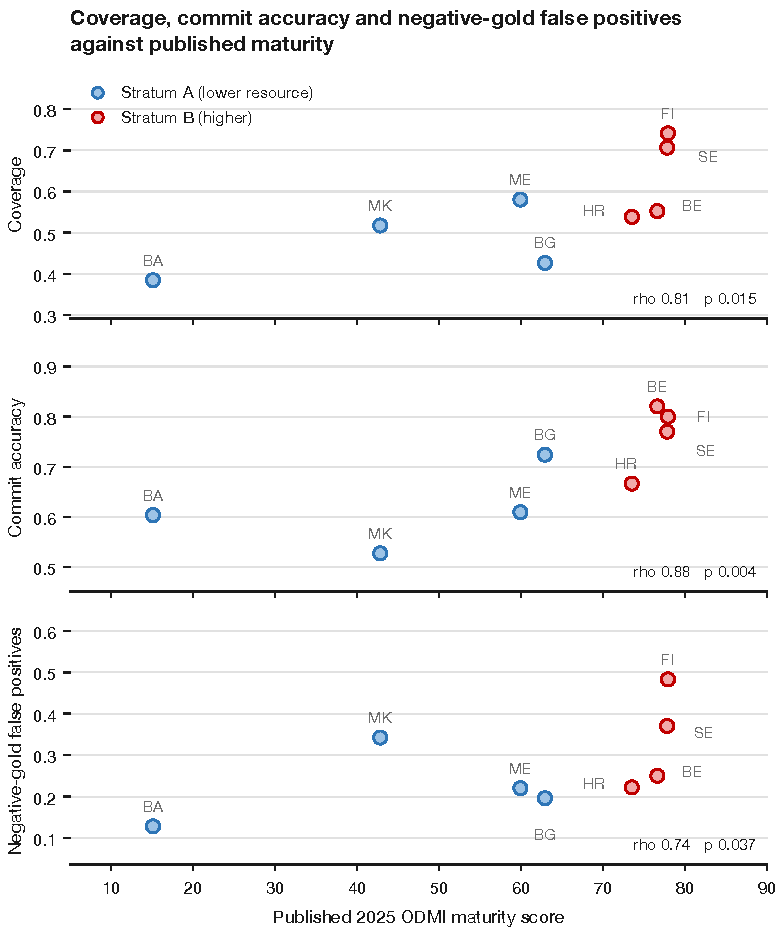
\includegraphics[width=0.72\linewidth]{figures/fig_4_5_maturity.pdf}
\caption{Coverage, commit accuracy and negative-gold false positives against published maturity.}
\label{fig:against-maturity}
\end{figure}

Finland records the highest false-positive rate of the eight countries, at 48.3\%, and Bosnia and Herzegovina the lowest, at 12.8\%, against published maturities of 77.9 and 15.1. Figure~\ref{fig:against-maturity} ranks every country with its published maturity, against coverage, commit accuracy and the false-positive rate, and all three climb with it, at Spearman correlations of 0.81, 0.88 and 0.74. North Macedonia is the exception, at 30.1\% on a maturity of 42.8, above four countries that score higher. The country figures rest on small counts at the mature end, where Belgium holds 24 negative golds and Finland 29, so the ordering is a tendency across the range rather than a difference between any two countries. The rate plotted here divides by every negative gold, including the ones the swarm declined, so a country that abstains more posts a lower one. Measured only on the negative golds it committed to, the correlation with maturity rises to 0.90. One explanation fits, though the present design cannot confirm it.

In mature countries, a negative gold rarely signifies a simple absence. Because such countries implement most practices, a recorded ``no'' is often accompanied by adjacent evidence, partial implementation, a related practice, or a published intention yet to be realised. This near-miss evidence is plentiful and can be interpreted as support for a positive answer. By contrast, in less mature countries a negative gold more commonly indicates a practice that is absent, and the open web yields little that could be confused with it, as they have a sparser web-presence. Section~\ref{sec:llm-limitations} outlines the mechanism by which adjacent evidence leads to over-reading. The denser the evidence base, the more material there is to over-read.

Section~\ref{sec:criteria} set out the requirement that a country\textquotesingle s result depends "solely on its capability in the specific quality that is being assessed". A distinction has to be made. Subgroup Equity requires that a country\textquotesingle s score tracks its maturity alone, whereas here, the swarm\textquotesingle s performance tracks maturity too. Subgroup Equity therefore is not met, and the reason sits in the current form of the assessment. The system recovers 87.0\% of the yes golds it commits to against 48.9\% of the no golds. A country\textquotesingle s maturity is calculated directly from how many answers are negative, so the class the system handles worst makes up a larger part of a low-maturity country\textquotesingle s assessment. A score is built from counts of awarded marks. Stratum A accrues 55 wrongly credited answers against stratum B\textquotesingle s 36, even though its rate per negative gold is the lower of the two. Coverage falls as maturity falls, which is the top panel of Figure~\ref{fig:against-maturity}. Among the answers that do commit, wrong yesses outnumber wrong noes by roughly two to one, so what survives leans towards crediting practices that are not there. Both effects track the country\textquotesingle s position on the scale the index exists to measure, which makes the error a function of the quantity the system intends to measure.

\section{Generalisability}\label{sec:generalisability}

Generalisability asks whether the system performs evenly across the question types and dimensions in the assessment, or whether it has weak points hidden by an aggregated accuracy figure. In the closest published analogue to this work, \textcite{fumega2026} set deep research agents to find evidence on the open web and answer a data-policy questionnaire from it. Their mismatch against the human answers runs from 19\% on the indicator whose evidence sits in a single document to 69\% on the one whose evidence is scattered, averaging 42\% across four indicators. The pooled commit-accuracy in Section~\ref{sec:convergent-validity}, 70.1\% over the 623 committed answers that carry a score, is the kind of figure that invites this question. The headline is therefore broken apart two ways: by ODMI dimension, and by the answer shape each question demands. 

\begin{figure}[htbp]
\centering
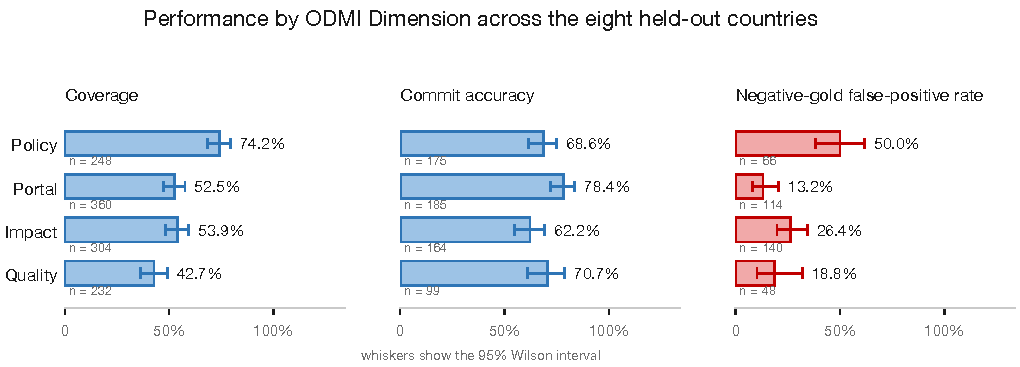
\includegraphics[width=\linewidth]{figures/fig_4_5_dimension.pdf}
\caption{The headline by dimension.}
\label{fig:by-dimension}
\end{figure}

Across the four dimensions the headline holds unevenly, as Figure~\ref{fig:by-dimension} sets out. Commit-accuracy runs from 78.4\% on Portal to 62.2\% on Impact, and coverage varies more, from 74.2\% on Policy to 42.7\% on Quality. Counting abstentions as failures the dimensions sit between 30.2\% for Quality and 48.4\% for Policy. The gap is largest on negative golds, with the false-positive rate at 13.2\% on Portal and 50.0\% on Policy.

Dimension and answer shape are not independent. The graded questions sit almost entirely in Quality, and the nine catalogue questions are most of why the dimension looks unreachable. The 50\% accuracy of the nine questions pull down the rest of the dimension, and once they are set aside the swarm answers Quality at 80.3\% when it commits, so the 70.7\% in Figure~\ref{fig:by-dimension} is the catalogue questions pulling the score down. Quality\textquotesingle s low coverage is the system declining what it cannot ground, which is also why its negative-gold false-positive rate is the second lowest of the four. Portal sits at the other extreme, strongest on both accuracy and false positives, because a portal\textquotesingle s features can be read straight off the portal, the one place where absence of proof does equate to absence of existence. Policy is the revealing case, it answers the most and gets half of its negative golds wrong.



\begin{figure}[htbp]
\centering
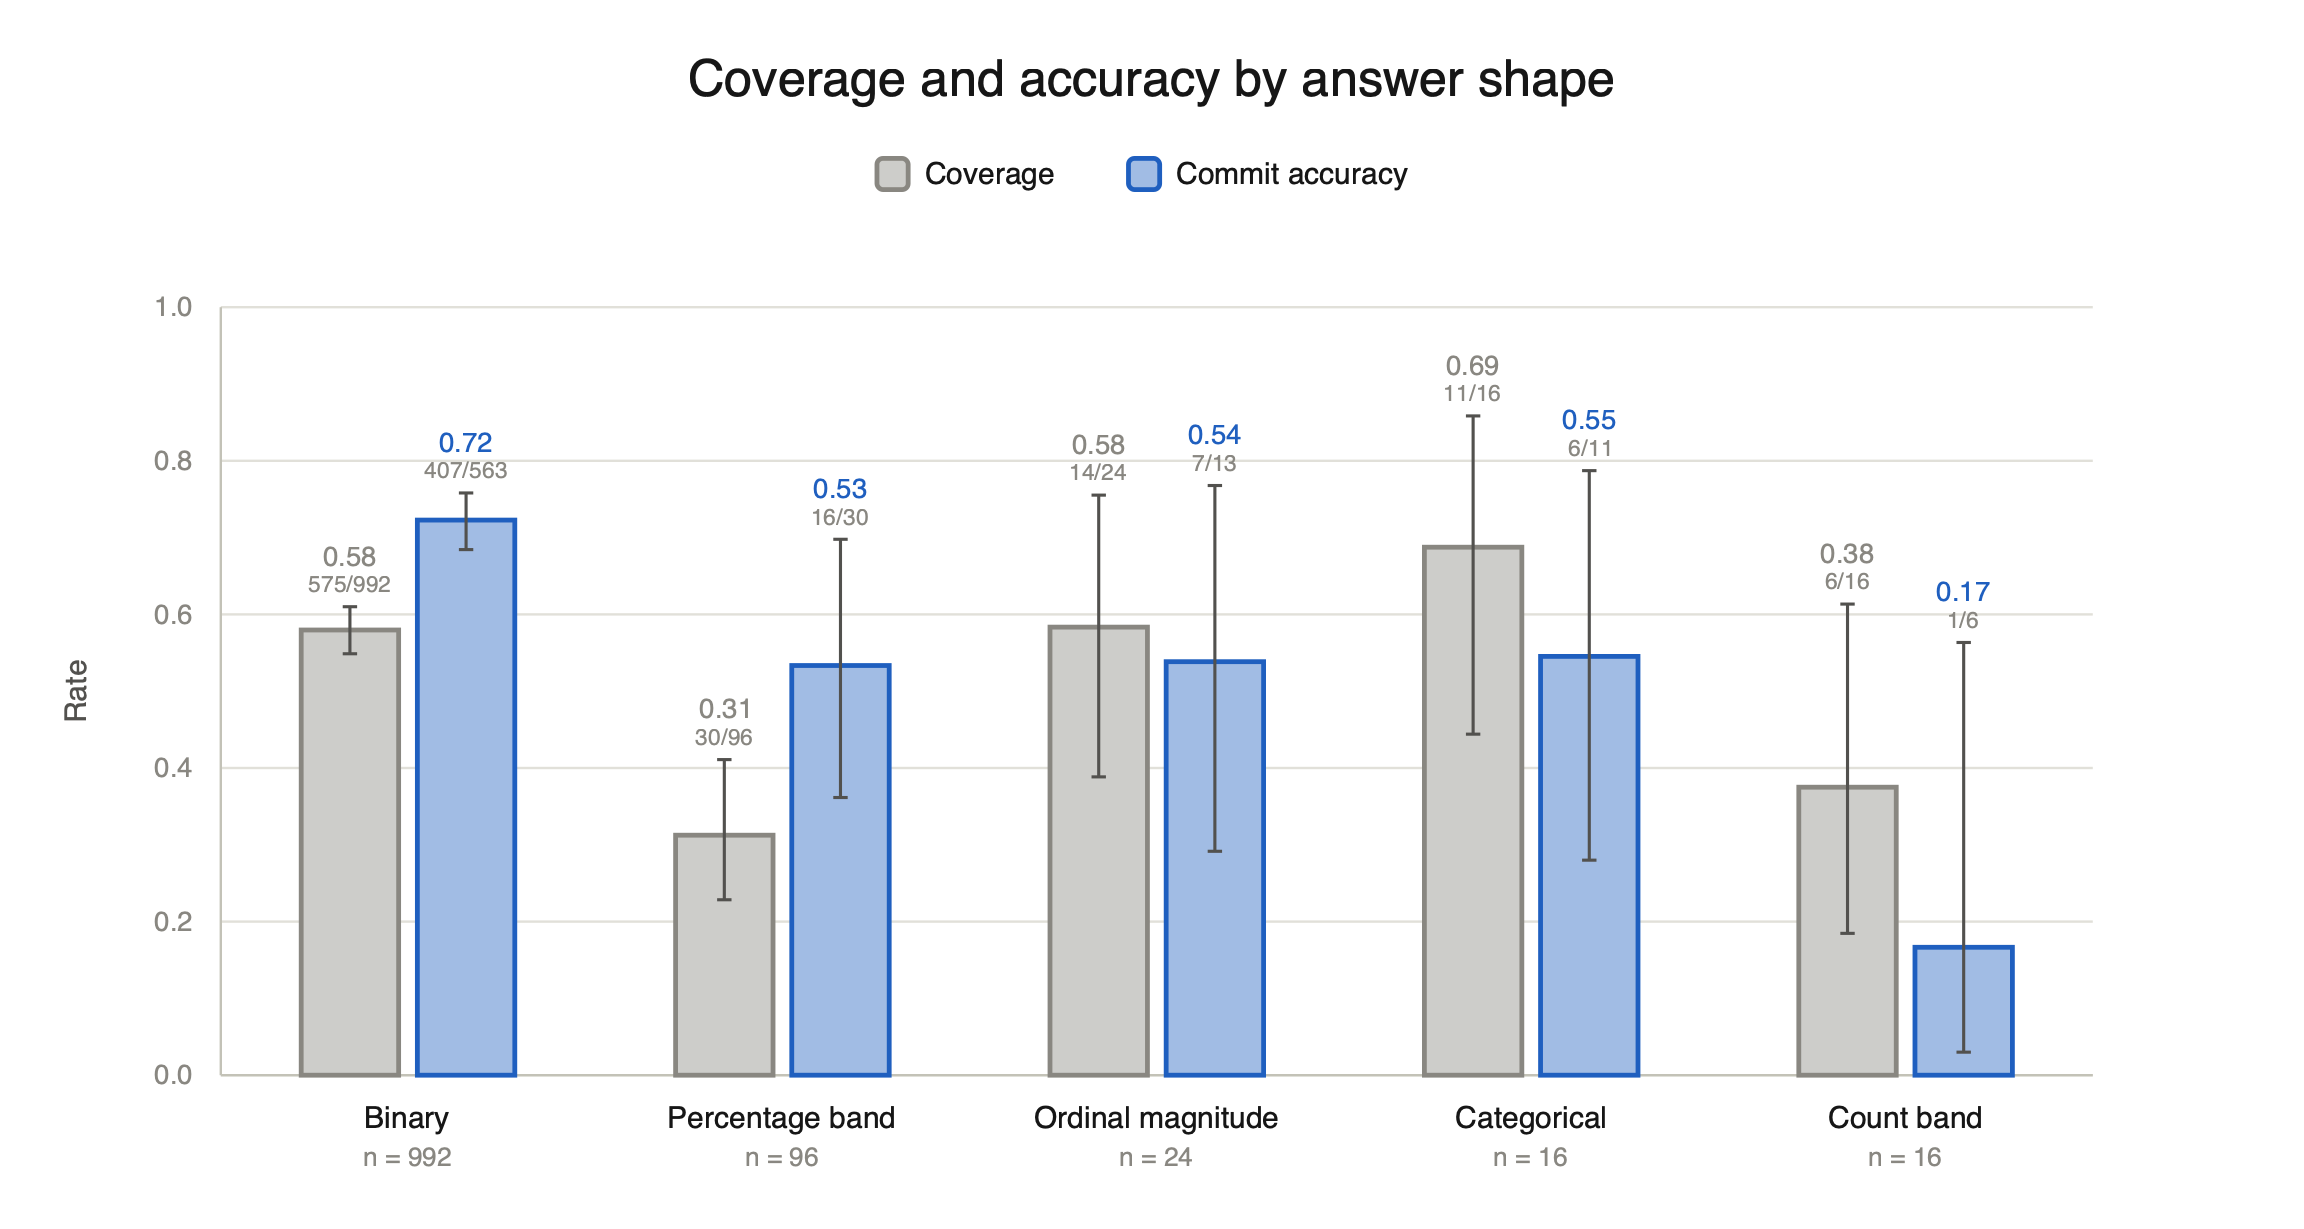
\includegraphics[width=\linewidth]{figures/coverage_accuracy_by_answer_shape.png}
\caption{Coverage and accuracy by answer shape.}
\label{fig:by-answer-shape}
\end{figure}

The spread by answer shape is wider, shown in Figure~\ref{fig:by-answer-shape}, with the nine computable Quality questions set aside. Binary question-country pairs reach 72.3\% commit-accuracy across 992 pairs. The four percentage-band questions outside that set, which ask for a proportion read off a web page, are declined on all 32 of their pairs, and the swarm gets 1 of the 16 count-band questions exactly right. The two shapes it attempts with any regularity, ordinal-magnitude and categorical, reach 29.2\% and 37.5\% over all their pairs, on only 24 and 16 pairs. The majority of what the questionnaire asks in a graded form is either declined or wrong.

Coverage and accuracy must be considered together, because a dimension that abstains from most questions can still achieve a high score on the few it retains. Section~\ref{sec:llm-limitations} set out why an agent constrained to reason from retrieved evidence would fail by over-interpretation, the system attributing evidence that may be adjacent, partial or ambiguous as proof. What varies across the assessment, affecting dimensions and countries alike, is the amount of evidence needed to prove a claim. Portal is the dimension where evidence is dispositive, since a portal feature is either present on the portal or it is not, and Portal is accordingly the strongest of the four on both accuracy and false positives. Policy is the dimension where evidence is abundant and rarely dispositive, since a draft strategy, an EU obligation or a regional initiative all resemble the national instrument the question asks about, and Policy commits most readily and returns a wrong yes on half of all its negative golds. Quality is the dimension where little evidence of any kind reaches the open web, and it declines most and stays second-cleanest on negatives. This is the ordering Section~\ref{sec:subgroup-equity} found across countries rather than questions. Finland, at 77.9 maturity, carries the highest false-positive rate in the run, and Bosnia and Herzegovina, at 15.1, the lowest. A mature country and a Policy question share a property, both hold a significant amount of published material that sits near the question without answering it. Section~\ref{sec:selectivity} shows the same asymmetry at the level of a single answer, where a ``yes'' needs a document and a ``no'' needs an absence that cannot be quoted. The system does not fail where evidence is scarce so much as where evidence is plentiful and beside the point.

\section{Reproducibility}\label{sec:reproducibility}

Reproducibility asks whether the same assessment, run again, returns the same answers. Section~\ref{sec:criteria} set two conditions: a record complete enough for the run to be repeated, covering the prompts issued, the evidence retrieved, the model version and the settings it ran under, and evidence that a repeat returns the same answers. The second matters most for a generative assessor, whose output varies across runs of the same prompt, where the score a country receives should depend only on its data openness.

The first condition holds with one gap. Every Researcher, Verifier and Adjudicator call writes a row carrying the prompt version, the snippets the Researcher read, the model version and the settings. The snippet picker, the model call that selects which passages from each fetched page reach the Researcher, writes no equivalent row for this run, so its prompt and model version sit outside the record. Its output is kept, since the picked snippets are stored against the Researcher call that used them, and the run therefore replays from the Researcher\textquotesingle s inputs onward rather than from every model call. The second condition must be measured between runs, to assess the stability of the answers.

\begin{longtable}[]{@{}
  >{\raggedright\arraybackslash}p{(\linewidth - 10\tabcolsep) * \real{0.1280}}
  >{\raggedright\arraybackslash}p{(\linewidth - 10\tabcolsep) * \real{0.1379}}
  >{\raggedright\arraybackslash}p{(\linewidth - 10\tabcolsep) * \real{0.1477}}
  >{\raggedright\arraybackslash}p{(\linewidth - 10\tabcolsep) * \real{0.1379}}
  >{\raggedright\arraybackslash}p{(\linewidth - 10\tabcolsep) * \real{0.1879}}
  >{\raggedright\arraybackslash}p{(\linewidth - 10\tabcolsep) * \real{0.2094}}@{}}
\caption{The three replicate runs.}\label{tab:replicates}\\
\toprule\noalign{}
\begin{minipage}[b]{\linewidth}\centering
\textbf{Replicate}
\end{minipage} & \begin{minipage}[b]{\linewidth}\centering
\textbf{Finalised}
\end{minipage} & \begin{minipage}[b]{\linewidth}\centering
\textbf{Commit rate}
\end{minipage} & \begin{minipage}[b]{\linewidth}\centering
\textbf{Committed}
\end{minipage} & \begin{minipage}[b]{\linewidth}\centering
\textbf{Commit Accuracy}
\end{minipage} & \begin{minipage}[b]{\linewidth}\centering
\textbf{Aggregate Accuracy}
\end{minipage} \\
\midrule\noalign{}
\endfirsthead
\toprule\noalign{}
\begin{minipage}[b]{\linewidth}\centering
\textbf{Replicate}
\end{minipage} & \begin{minipage}[b]{\linewidth}\centering
\textbf{Finalised}
\end{minipage} & \begin{minipage}[b]{\linewidth}\centering
\textbf{Commit rate}
\end{minipage} & \begin{minipage}[b]{\linewidth}\centering
\textbf{Committed}
\end{minipage} & \begin{minipage}[b]{\linewidth}\centering
\textbf{Commit Accuracy}
\end{minipage} & \begin{minipage}[b]{\linewidth}\centering
\textbf{Aggregate Accuracy}
\end{minipage} \\
\midrule\noalign{}
\endhead
\bottomrule\noalign{}
\endlastfoot
Run 1 & 155 / 156 & 46.6\% & 69 & 69.1\% & 31.8\% \\
Run 2 & 154 / 156 & 44.6\% & 66 & 67.7\% & 29.7\% \\
Run 3 & 151 / 156 & 50.0\% & 74 & 68.5\% & 33.8\% \\
\end{longtable}


Three fresh dispatches of the swarm ran over the 156-pair development battery, with nothing seeded or replayed and the search cache purged before each run, so every replicate found its evidence from scratch. Table~\ref{tab:replicates} gives each run; the eight pairs between the runs that didn't finalise were search stalls, disclosed and excluded, so the analysis rests on the 148 pairs present in all three.

The decision to answer is the unstable part of the system and the answer itself is stable. All three runs reached the same outcome on 70.3\% of the 148 pairs. Commit accuracy moves across a range of 1.4 points while roughly 30\% of pairs change outcome between runs, so disagreements at the level of individual questions largely cancel once they are pooled into a rate. So the official maturity score a country receives may be stable between runs, with a third of underlying evidence varying.

The asymmetry between the two gold classes sits entirely in the decision to answer. Outcome unanimity is 60.5\% on negative golds against 80.0\% on positive ones. The higher variance in negative golds reflects the clustering near and below the confidence threshold from Section~\ref{sec:selectivity}, and pairs that changed outcome between the runs had a median confidence of 0.68, with 44.6\% of them sitting exactly at 0.65. These sparse-evidence pairs are more likely to drop below the threshold than the well-evidenced ``yesses'' that hold between runs. Once all three replicates commit they agree on the label on 47 of 51 pairs, 92.2\%, and that rate holds within both gold classes. What varies with the evidence available is whether the system answers, not the answer it gives.



\begin{figure}[htbp]
\centering
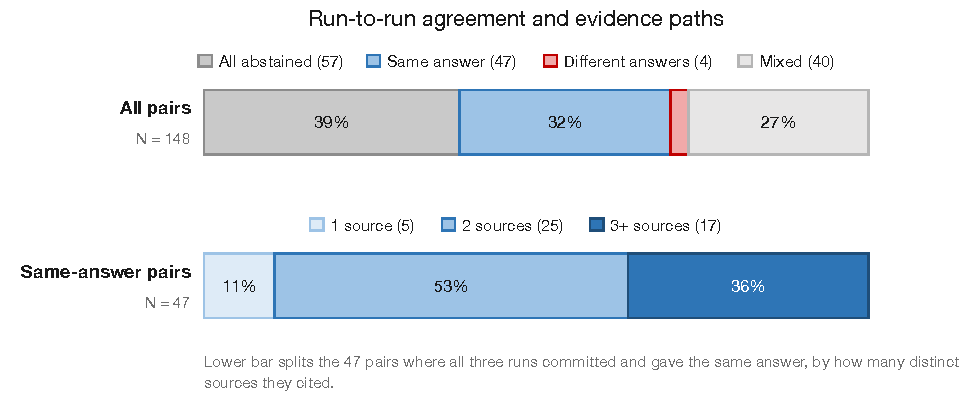
\includegraphics[width=\linewidth]{figures/fig_4_7_1_runtorun.pdf}
\caption{Outcome agreement across the three replicate runs, and the distinct sources cited on the pairs where all three agreed.}
\label{fig:replicates-fig}
\end{figure}

The route to those answers varied far more than the answers did, as the lower bar of Figure~\ref{fig:replicates-fig} shows. Of the 47 pairs where all three replicates committed and agreed, 42 cite two or more distinct source URLs across the runs and 17 cite three. Section~\ref{sec:criteria} anticipated this, that a generative assessor finding its own evidence may issue different queries and read different pages between runs when the underlying truth has not changed, and that what has to hold is the outcome whatever route the model took to it.

Against the two conditions of Section~\ref{sec:criteria}, the record replays and the published score is stable, but the individual question decisions are not. The instability is in whether the system answers a given question at all, and it falls on the thin-evidence negative golds whose confidence sits at the 0.65 floor, where a small shift between runs tips the decision either way. This does not reach the score. A country\textquotesingle s score pools 143 questions, the per-question flips offset each other, and commit accuracy moves only 1.4 points across the three runs. So the number the ODMI would publish is reproducible, but the stability of the evidence for each question varies.

\section{Ablation}\label{sec:ablation}

Each component of the swarm was removed in turn to test what it contributes. The ablation runs on the eight evaluation countries, and four arms are compared. The Researcher alone commits when its own confidence is sufficient, with no second call. The second arm adds the Adversarial Verifier and its retry loop, committing only where the two agents agree within three retries. The third is the full swarm, with the Adjudicator arbitrating disagreements. The fourth replaces the Adversarial Verifier with a corroborative one, prompted to find evidence supporting the Researcher\textquotesingle s claim rather than against it. This arm has no adjudicator, both because a corroborative check produces at most an absence of support rather than a counterargument to weigh, and because the arm exists to isolate the Verifier\textquotesingle s stance.

\begin{longtable}[]{@{}
  >{\raggedright\arraybackslash}p{(\linewidth - 10\tabcolsep) * \real{0.2183}}
  >{\raggedright\arraybackslash}p{(\linewidth - 10\tabcolsep) * \real{0.1776}}
  >{\raggedright\arraybackslash}p{(\linewidth - 10\tabcolsep) * \real{0.1776}}
  >{\raggedright\arraybackslash}p{(\linewidth - 10\tabcolsep) * \real{0.1929}}
  >{\raggedright\arraybackslash}p{(\linewidth - 10\tabcolsep) * \real{0.1269}}
  >{\raggedright\arraybackslash}p{(\linewidth - 10\tabcolsep) * \real{0.1066}}@{}}
\caption{The ablation ladder. Four arms over the 1,144 evaluation pairs, Sonnet 4.6.}\label{tab:ablation}\\
\toprule\noalign{}
\begin{minipage}[b]{\linewidth}\raggedright
\textbf{Configuration}
\end{minipage} & \begin{minipage}[b]{\linewidth}\raggedright
\textbf{Commit rate}
\end{minipage} & \begin{minipage}[b]{\linewidth}\raggedright
\textbf{Commit accuracy}
\end{minipage} & \begin{minipage}[b]{\linewidth}\raggedright
\textbf{Negative-gold FP rate}
\end{minipage} & \begin{minipage}[b]{\linewidth}\raggedright
\textbf{Balanced acc.}
\end{minipage} & \begin{minipage}[b]{\linewidth}\raggedright
\textbf{Youden J}
\end{minipage} \\
\midrule\noalign{}
\endfirsthead
\toprule\noalign{}
\begin{minipage}[b]{\linewidth}\raggedright
\textbf{Configuration}
\end{minipage} & \begin{minipage}[b]{\linewidth}\raggedright
\textbf{Commit rate}
\end{minipage} & \begin{minipage}[b]{\linewidth}\raggedright
\textbf{Commit accuracy}
\end{minipage} & \begin{minipage}[b]{\linewidth}\raggedright
\textbf{Negative-gold FP rate}
\end{minipage} & \begin{minipage}[b]{\linewidth}\raggedright
\textbf{Balanced acc.}
\end{minipage} & \begin{minipage}[b]{\linewidth}\raggedright
\textbf{Youden J}
\end{minipage} \\
\midrule\noalign{}
\endhead
\bottomrule\noalign{}
\endlastfoot
Closed book (no retrieval) & 75.6\% (865/1144) & 55.3\% (476/860) & 13.9\% (51/368) & 0.429 & -0.143 \\
Researcher alone & 26.6\% (304/1144) & 74.3\% (220/296) & 12.5\% (46/368) & 0.173 & -0.653 \\
+ adversarial Verifier & 46.0\% (526/1144) & 72.5\% (372/513) & 23.4\% (86/368) & 0.315 & -0.370 \\
+ Adjudicator (full trio) & 55.6\% (636/1144) & 70.1\% (437/623) & 24.7\% (91/368) & 0.396 & -0.208 \\
Corroborative Verifier & 47.6\% (545/1144) & 71.2\% (380/534) & 27.2\% (100/368) & 0.316 & -0.368 \\
\end{longtable}


Table~\ref{tab:ablation} shows the results of this ablation ladder, covering commit rate, accuracy and negative-gold false-positive rate. The headline result is the improvement in coverage rather than raw accuracy. The Researcher alone commits on 26.6\% of the pairs, lifting to 46.0\% with the Adversarial Verifier and 55.6\% with the Adjudicator. The number of correct answers rises with it, from 220 to 372 to 437 out of 1,144. The Verifier turns 165 of the Researcher\textquotesingle s wrong or withheld answers into correct ones and loses 13 the other way, and the Adjudicator adds 65 correct answers while reversing none.

Accuracy on the answers each arm keeps moves the other way. The Researcher alone reproduces the published key on 74.3\% of what it commits, the Adversarial Verifier arm on 72.5\%, and the full trio on 70.1\%. The closed-book floor commits readily, on 75.6\% of pairs, and reproduces the key on 55.3\% of them, so the evidence the swarm gathers is worth fifteen points of commit accuracy over the model\textquotesingle s own priors.

That gap closes once both are made to answer everything. Scoring every binary question and counting a declined one as wrong, the closed-book model reproduces 43.0\% of the key and the full swarm 42.4\%. Retrieval does not raise the number of questions the system gets right. It raises the share it gets right among the ones it keeps, which is a claim about selection and not about knowledge.

Two results complicate this picture. The first is that the Adversarial Verifier does not filter for precision. If it did, it would commit fewer wrong answers on the negative golds than the Researcher alone. It commits more. Coverage rises from 26.6\% to 46.0\% and the false-positive rate climbs with it, from 12.5\% to 23.4\%. The Adjudicator raises coverage again to 55.6\%, adding five further wrong commitments on the negative golds and recovering none, which leaves the rate almost unmoved at 24.7\%. That it costs so little supports Tyen et al.\textquotesingle s finding that a model rules on a located error far more reliably than it detects one unaided, since the Adjudicator only ever sees a disagreement the Verifier has already drawn. The closed-book floor puts the problem at its sharpest. Answering from its parameters alone, it asserts a wrong yes on 13.9\% of the negative golds against the full trio\textquotesingle s 24.7\%, so a model with no evidence in front of it commits fewer false yeses than the architecture built to prevent them.

The obvious objection is that the closed-book model only looks precise because it declines more of the hard questions. It does not. It commits on 56.8\% of the negative golds where the full swarm commits on 50.0\%, so it answers more of them and still recovers 42.1\% of the no answers against the swarm\textquotesingle s 24.5\%. Searching the web nearly halves the system\textquotesingle s ability to establish that a practice is absent. The likely reason is what a search returns. Material adjacent to a practice reads as evidence that the practice exists, and nothing comes back that evidences its absence. This comparison cannot prove that on its own, since the closed-book arm differs from the Researcher in its prompt, its lack of a confidence gate and its lack of a Verifier, so a readier disposition to answer ``no'' is not ruled out.

The two are also right about different questions. Across the binary golds they agree on 243 and disagree on 289, with 142 going to the swarm and 147 to the closed-book model, at a McNemar p of 0.8140. A system able to pick the better of the two on each question would reach 58.7\%, well above either alone. Retrieval and parametric recall are close to independent here, which this design was not built to exploit.

The second result is that the Verifier\textquotesingle s stance does not matter. Swapping the Verifier from adversarial to corroborative changes very little. Balanced accuracy moves from 31.5\% to 31.6\%. Of the 110 pairs one arm answered correctly and the other did not, 51 went to the adversarial arm and 59 to the corroborative, at a McNemar p of 0.5047. On total accuracy, which counts an abstention as a miss, the arms sit at 32.5\% and 33.2\%, a difference of 0.7 points against a paired standard error of 0.9, and this is evidence of equivalence. Section~\ref{sec:verification-methods} and Section~\ref{sec:debate} argue that opposition succeeds where corroboration fails in a thin-evidence setting, because corroboration compounds the model\textquotesingle s guessing bias while refutation checks it. On accuracy that argument is not supported.

It survives on the negative golds, where the adversarial arm commits a wrong answer on 23.4\% against the corroborative arm\textquotesingle s 27.2\%, and of the 50 where exactly one arm went wrong, 32 came from the corroborative arm, at p of 0.0649. Corroboration raises yes-recall from 52.1\% to 55.8\% and lowers no-recall from 10.9\% to 7.3\%, the guessing bias Section~\ref{sec:debate} describes, short of significance.

The literature anticipates this. \textcite{chowdhury2026} assign a different model to each of their judges, on the argument that agents drawn from the same weights cannot be relied on to disagree. Their own ablation locates the largest single gain not in the argumentation structure but in progressive evidence retrieval, 7.5 points of their 10.0-point improvement over standard multi-agent debate. \textcite{zhu2026} attribute the benefit of debate to agent diversity rather than to the framework itself. Here the Researcher and Verifier are the same Claude model, so the change in stance is a prompt difference and nothing more, and a prompt difference producing an equivalence result is what this literature would predict.

Both halves point the same way, and it is the conclusion Section~\ref{sec:selectivity} and Section~\ref{sec:attributability} reach from other directions, that every mechanism built to control precision acted on coverage instead.

\section{Operational Cost and Runtime}\label{sec:cost-runtime}

Section~\ref{sec:criteria} set timeliness and cost-effectiveness aside from the six criteria, since neither addresses whether the automation upheld the legitimacy previously assumed by the human rater. Both still matter for whether automation is worth running at all, given the labour a 5,148-question assessment demands.

One caveat governs every figure below. The system runs through a local proxy against a flat subscription, so the marginal cost of a run is zero and the sterling amounts are notional, converting logged tokens at published list prices to give what the same work would cost on a metered API. The figures cover every model call the pipeline makes. The three agents account for 23\% of the spend, the remaining 77\% goes to the snippet picker, the call that reads each fetched page and selects the passages the Researcher reasons over (Section~\ref{sec:retrieval}). The system spends over three times as much reading pages as it does reasoning about what it read.

Answering all 1,144 evaluation pairs cost £375 in notional compute, spread across the denominators of Table~\ref{tab:cost}: £0.33 per attempted pair, £0.59 per answer given, and £0.86 per answer that matched the key, of which there were 437.

\begin{longtable}[]{@{}
  >{\raggedright\arraybackslash}p{(\linewidth - 4\tabcolsep) * \real{0.5556}}
  >{\raggedright\arraybackslash}p{(\linewidth - 4\tabcolsep) * \real{0.1944}}
  >{\raggedright\arraybackslash}p{(\linewidth - 4\tabcolsep) * \real{0.2500}}@{}}
\caption{What the assessment cost.}\label{tab:cost}\\
\toprule\noalign{}
\begin{minipage}[b]{\linewidth}\raggedright
\textbf{Basis}
\end{minipage} & \begin{minipage}[b]{\linewidth}\raggedright
\textbf{Pairs}
\end{minipage} & \begin{minipage}[b]{\linewidth}\raggedright
\textbf{Cost per pair}
\end{minipage} \\
\midrule\noalign{}
\endfirsthead
\toprule\noalign{}
\begin{minipage}[b]{\linewidth}\raggedright
\textbf{Basis}
\end{minipage} & \begin{minipage}[b]{\linewidth}\raggedright
\textbf{Pairs}
\end{minipage} & \begin{minipage}[b]{\linewidth}\raggedright
\textbf{Cost per pair}
\end{minipage} \\
\midrule\noalign{}
\endhead
\bottomrule\noalign{}
\endlastfoot
Every pair attempted & 1,144 & £0.33 \\
Pairs the swarm answered & 636 & £0.59 \\
Answers matching the key & 437 & £0.86 \\
A pair it committed to & 636 & £0.28 \\
A pair it abstained on & 508 & £0.41 \\
Whole evaluation run & 1,144 & £375 total \\
\end{longtable}


These figures are averages; pair cost varies with the number of calls required. A pair that the system committed to cost £0.26 and required 2.2 attempts, whereas a pair on which it abstained cost £0.41 and used the full three-retry budget, because under the loop described in Section~\ref{sec:agent-loop} a pair reaches abstention only after all retries are exhausted. Section~\ref{sec:selectivity} argued that abstention is the honest outcome when evidence is thin, and this is the cost of that honesty. Selectivity is the most expensive result for a pair.

Per-country cost is nearly flat, from £0.310 in Finland to £0.348 in Bosnia and Herzegovina, up to £0.385 with Bulgaria, and most of that spread is the abstention mix rather than anything about how hard a country\textquotesingle s evidence is to read. Bosnia abstains on 61.5\% of its pairs against Finland\textquotesingle s 25.9\%, and an abstained pair costs 58\% more than a committed one does. Set against Section~\ref{sec:subgroup-equity}, where coverage, commit accuracy and the false-positive rate all track published maturity, cost is the one measure that does not.\textbf{ }

Model choice is the other lever, and Appendix~\ref{app:experiments} gives the comparison across Haiku 4.5, Sonnet 4.6 and Opus 4.8 on the development battery. It moves how much the system is willing to say, rather than how often it is right. Sonnet is retained because it commits most, at a middling price, with commit-accuracy indistinguishable from Opus, which costs over three times as much.

A pair took a median of 200 seconds from its first logged Researcher call to its finalised row, counting the searches issued and the pages fetched alongside the model\textquotesingle s own work, and 95\% finished inside six minutes. This is an upper bound under load, since up to twenty pairs ran simultaneously on one machine competing for the same connection. Three pairs ran past thirty minutes, the longest at forty-nine, each stalled on an unresponsive server with the Swedish catalogue endpoint worst among them.

The eight evaluation countries took 45 hours and £375, so all 36 extrapolate to roughly 200 hours and £1,700. The time is an upper bound, since the eight were chosen to oversample negative golds, which skews them below the European average on maturity, and Section~\ref{sec:subgroup-equity} found lower-maturity countries abstain more, sending more pairs through the full retry budget.

This £1,700 does not buy a completed assessment, as the coverage across the eight countries is 55.6\%. The system would commit to around 2,860 of the 5,148 pairs and decline the other 2,290. Of the answers it commits to, 70.1\% match the published key. In practice, if this system ran as a precursor to human judgement, an assessor following it would have two populations to work on. The 2,290 declined pairs arrive as a visible queue, flagged and easy to route. The harder population is the 850 or so committed answers that are wrong, which look ostensibly identical to the correct answers, with the same structure of quote and source as the 2,010 that are right.

\section{Reconstructing the Index}\label{sec:reconstruction}

The point of this exercise is to see whether a human-labour-intensive process could be replaced by an automated one. This section constructs what the maturity score would be across the eight evaluation countries, and what work would be left for the humans overseeing the automation.

The ODMI computes each country\textquotesingle s score as the unweighted mean of four dimension percentages, each the marks awarded across its questions divided by the marks available. The rubric is not published but is recoverable from the answer key, at 345 distinct answer-to-score mappings across the 143 questions. Applying it to the published answers reproduces the 2025 figures exactly, at 100.0 for France and 62.9 for Bulgaria, which establishes that the recovered rubric reconstructs the ODMI\textquotesingle s arithmetic. Where the swarm returns an answer the rubric does not recognise, that answer scores zero.

Abstention makes the result a range rather than a figure. The floor scores every abstention as zero, and represents what a country could be awarded on public evidence alone. The ceiling scores only the pairs the swarm committed to, so it assumes the declined pairs would have scored at the same rate. That is optimistic, since Section~\ref{sec:selectivity} showed the swarm abstains on the questions it finds hardest.



\begin{figure}[htbp]
\centering
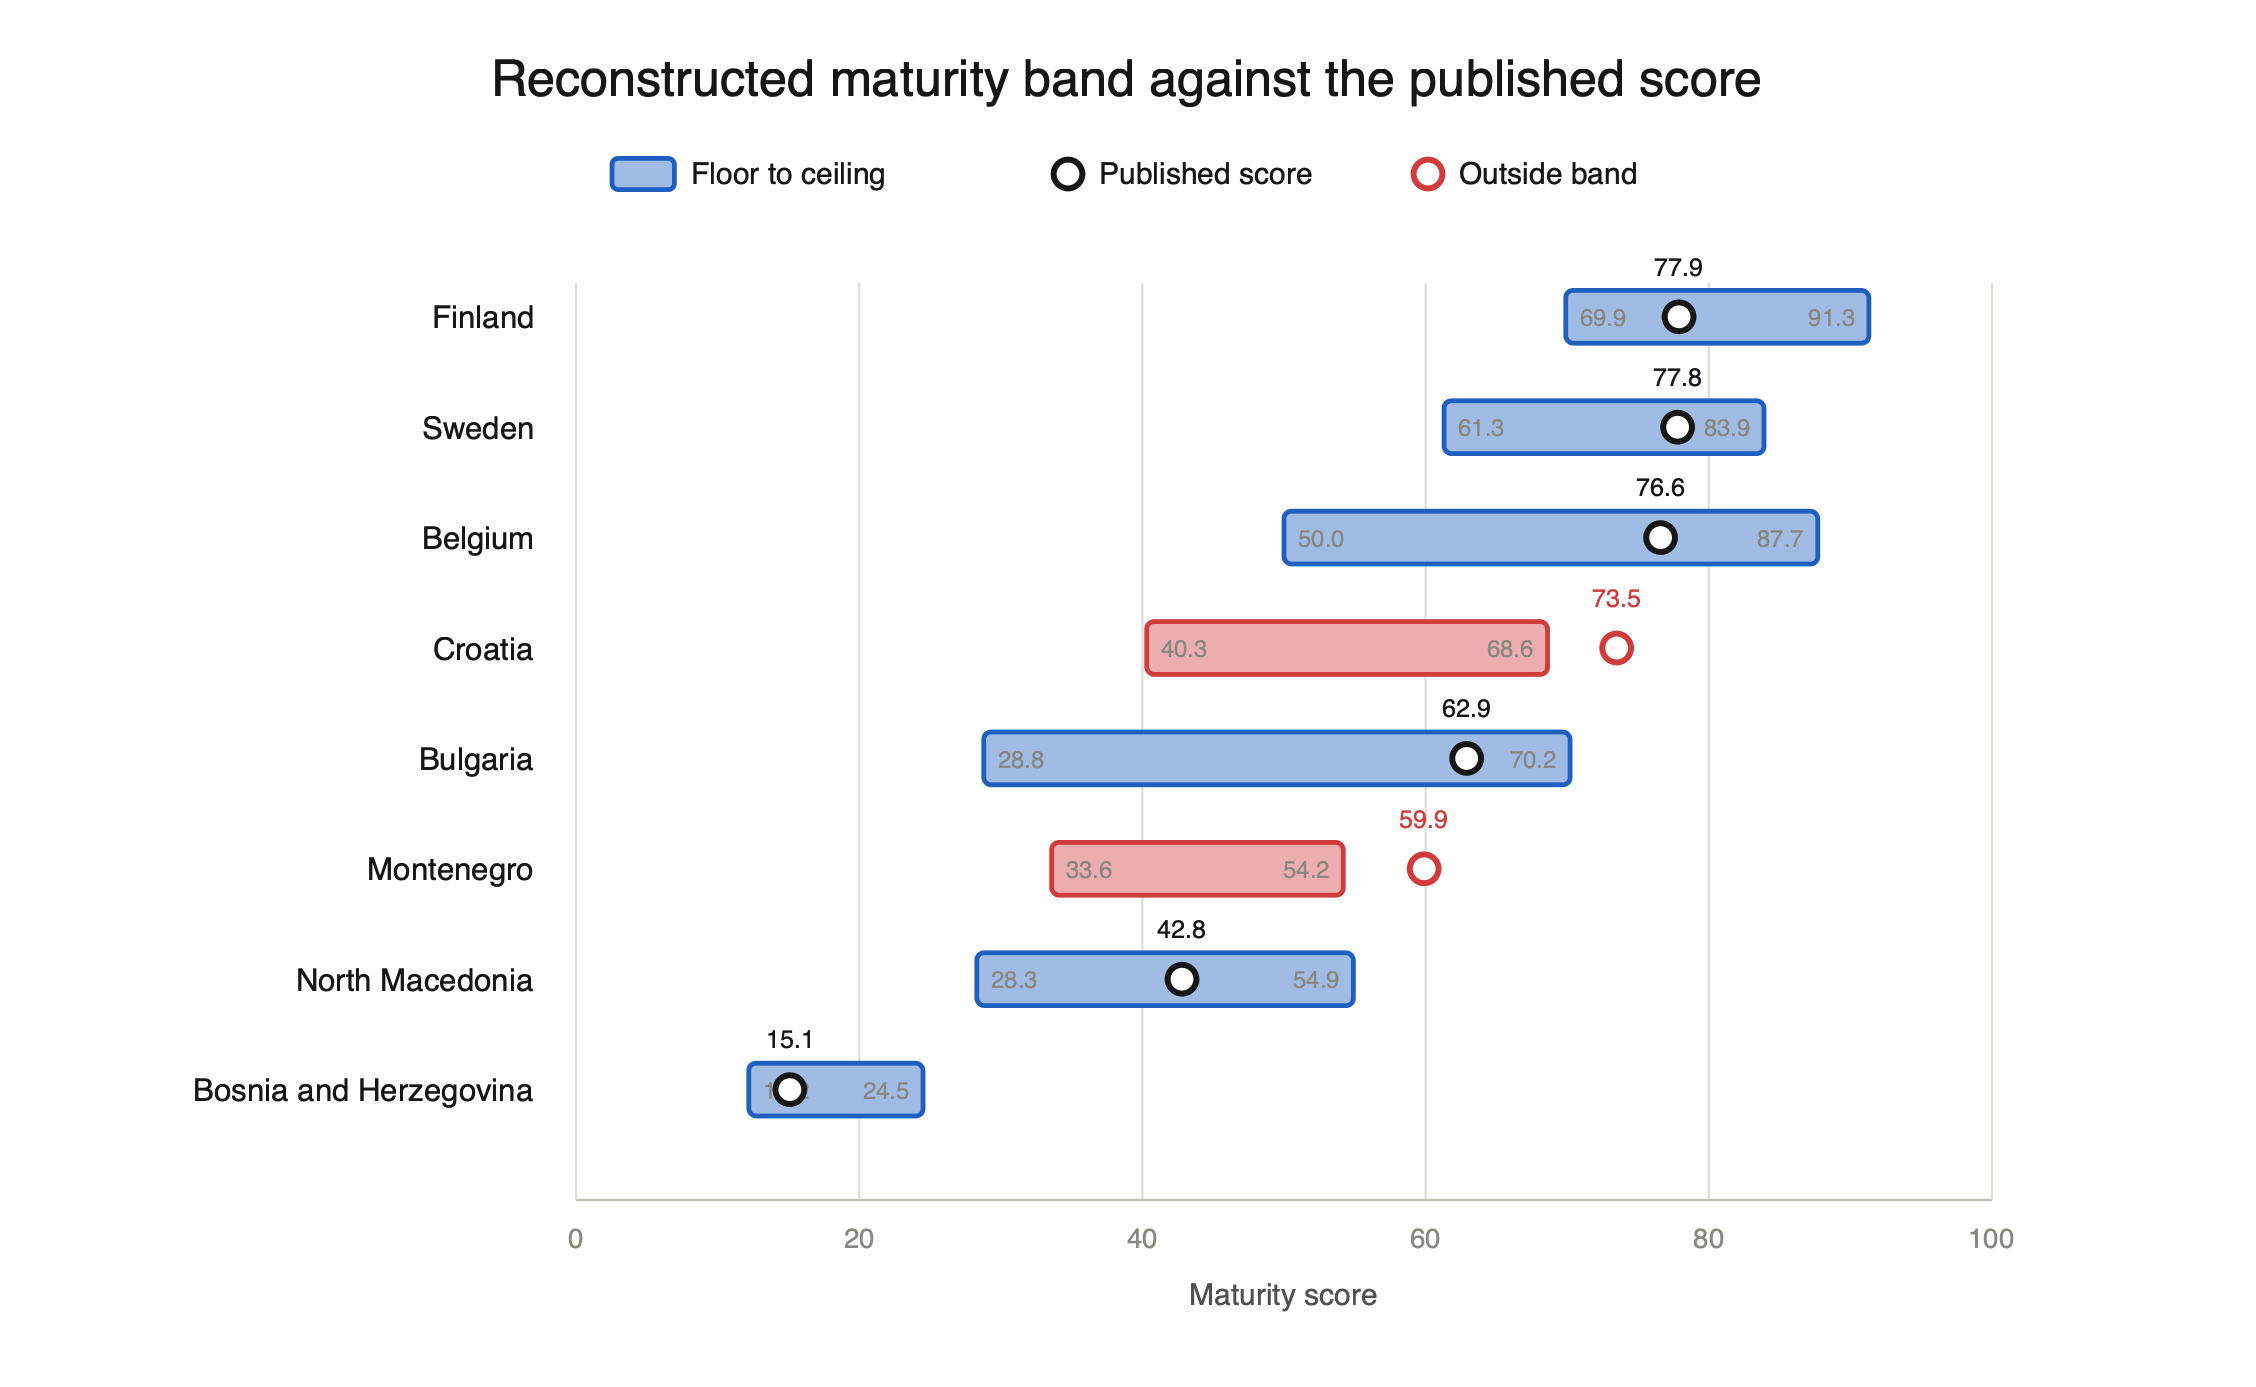
\includegraphics[width=\linewidth]{figures/reconstructed_band.png}
\caption{Reconstructed maturity band against the published score.}
\label{fig:reconstruction-fig}
\end{figure}

Ranking the eight by their reconstructed ceiling and comparing to the published order gives a Spearman correlation of 0.929, and on the floor 0.976. Section~\ref{sec:subgroup-equity} found coverage tracking published maturity at ρ = 0.81, and the floor is depressed by abstention, so a low-maturity country is pushed down the floor ordering by declining more as well as by scoring less. The ceiling removes that effect, since it divides only by what the swarm attempted. Per-country commit accuracy ranges from 52.8\% to 82.1\% and coverage from 38.5\% to 74.1\%, so there was ample room for the ordering to scramble, and yet it largely survived. The mean band spans 26.4 points and the published score falls inside it for six of the eight countries, as Figure~\ref{fig:reconstruction-fig} shows.

Two countries fall outside their band, and in the same direction. Croatia\textquotesingle s published 73.5 sits above a ceiling of 68.6, and Montenegro\textquotesingle s 59.9 above a ceiling of 54.2. In both cases the swarm cannot reach the published figure even crediting every declined question as though it had performed like the ones the swarm answered.

The ODMI states four purposes for the assessment: to help a country understand its own maturity, to capture its progress year on year, to identify areas for improvement, and to benchmark its performance against other countries. Benchmarking is recovered, as the swarm orders the eight countries almost exactly as the assessors do, and it does so on public evidence alone.

Understanding their own maturity is partly recovered. Where the swarm commits, it agrees with the published answer 70.1\% of the time, so a country reading the individual answers gets a substantially accurate picture of what an external assessor found. However, aggregating 143 of those into a single figure is where the precision goes, and the 26-point average band shows this.

Identifying areas for improvement depends on which area. Section~\ref{sec:generalisability} found the swarm reliable on Portal, at 78.4\% commit accuracy with a 13.2\% false-positive rate, so a Portal shortfall is worth acting on. Policy is the reverse: it commits most readily and returns a wrong yes on half its negative golds, so a Policy pass carries little information. A country acting on this output would need the per-dimension reliability published alongside it.

Year-on-year progress is out of reach on two counts. A country typically moves a few points a cycle, well inside a 26-point band, and Section~\ref{sec:reproducibility} found the per-question decision unstable across runs, so a difference between two cycles would carry sampling variation alongside real change.

The nine sections above describe one constraint. The swarm reproduces the published key on 70.1\% of the answers it commits to, against 43\% for the same model with no retrieval at all, and it reaches that figure by declining 44\% of the questions. Forced to answer everything, it falls below a blanket yes. The system declines half the questions whose answer is no against 37.1\% of those whose answer is yes, and each criterion above records a different consequence of that. Confidence measures how easy a claim was to evidence rather than how likely it is to hold. The two mechanisms built to control precision both acted on coverage. The error rises with a country\textquotesingle s published maturity, so it tracks the quantity the index exists to estimate. The searches themselves worked, and no abstention in this run came from an empty search. The system found material and could not turn it into evidence of an absence. Chapter~\ref{ch:discussion} takes up what would have to change, in the architecture and in the questionnaire, for a ``no'' to be evidenced on the same terms as a ``yes''.

\chapter{Discussion}\label{discussion}

This chapter reads the verdicts of §4 as a single account, returns to what the adversarial design contributed, then turns from the swarm to the questionnaire. It closes with the threats to the figures reported.

\section{The Scorecard}\label{the-scorecard}

The six criteria were introduced in §2.2 as the conditions under which an automated assessment stays contestable, and Chapter 4 returned a verdict on each. Read individually, those verdicts show multiple failure modes: abstention tracking maturity, correct negatives clustering below the confidence threshold, answer variance between runs. Read together, they describe a single constraint that affects everything downstream, data availability. This section works through the criteria in the order that makes that constraint visible, starting from the result most in need of explanation. The system reproduces the human process closely on the answers it commits to, yet when it is forced to answer every question its accuracy falls below what a fixed reply of yes would score. Its competence is therefore real but conditional on being allowed to decline, and what follows sets out what it is declining and why.

Convergent Validity establishes that there is agreement with the key, under certain conditions. On the pairs it commits to, the system agrees with the published key about seven times in ten, which is close reproduction of the existing process, but that figure holds only because it first sets aside almost half of the questions. The system recovers most of the positive answers and few of the negative ones, so the accuracy it reaches in normal operation is bought by declining the questions whose true answer is no. This locates the weakness exactly, and @@CL@@this is the optimism bias §2.3 anticipated@@/CL@@. It raises the question of why the system cannot commit a negative answer as reliably as a positive one.

Selectivity supplies the reason, and the reason is structural. The confidence score the system attaches to an answer measures how well the retrieved evidence supports the label it chose, and that quantity is not symmetric across the two labels. A positive answer can be evidenced directly, a negative answer has no equivalent, because the absence of a practice leaves nothing to quote. Confidence therefore tracks how easily a claim could be evidenced rather than how likely it is to hold, the asymmetry of Figure 4.2.2, and negative answers often sit under the commit threshold whatever their merit. The calibration results bear this out, with the system well behaved on positive golds and inverted on negative ones, most confident on the negatives at the point where it is most often wrong. The abstention seen under Convergent Validity is the system declining the answers it cannot evidence, which is the behaviour the criterion asks for, and it leaves the negative class structurally underserved.

Attributability removes the innocent reading of those errors, the possibility that the system is simply inventing them. The first of its two conditions, that a quoted passage exists in the retrieved text, is enforced mechanically before any answer commits, and every committed answer in the run satisfied it. Fabrication is therefore not the failure mode, and the positive answers the system commits are grounded in text it retrieved. What this leaves is more nuanced, because the wrong positives are drawn from real material that sits near the question. The system finds a relevant document, quotes a tangential passage, and reads it as proof. The second condition, that a reader would agree the passage supports the claim, is the one the Verifier set out to enforce, and it is where the remaining error lives.

Generalisability shows that this over-reading is not uniform but scales with how much adjacent material a question attracts. Where the evidence is dispositive the system is strong, and the portal dimension is the clearest case, since a portal feature is either present on the page or it is not and there is little room to over-read. Where the evidence is abundant without being decisive the system is weakest, and the policy dimension is the clearest case of that, since a draft strategy, an unadopted obligation or a regional initiative all resemble the national instrument a question asks about closely enough to be taken for it. Policy accordingly commits more readily than any other dimension and returns a wrong positive on half of its negative questions. This extends to the poor performance on all non-binary questions. The swarm declines almost everything that asks for a graded or computed figure, since those questions rarely offer a single passage that settles them.

Subgroup Equity carries the same mechanism from questions to countries. The stratification was built to detect a language effect, on the expectation that weaker comprehension of a national language would produce confident error, and that effect did not appear. What appeared instead is that measurement error tracks maturity. A mature country does most things, so a question whose true answer is no is still surrounded by adjacent evidence of related practices, and the open web returns abundant material that reads as support for yes. A less mature country more often lacks the practice outright, and the web returns little that could be mistaken for it. The false-positive rate consequently rises with a country\textquotesingle s published maturity while coverage falls as maturity falls, the two panels of @@CC@@Figure 5.1@@/CC@@, so a country\textquotesingle s assessed result depends in part on where it already sits on the scale the index exists to measure. An error that correlates with the quantity being estimated is a bias rather than noise, and the distinction matters for what follows, because noise averages out when many questions are pooled into a score and bias does not.

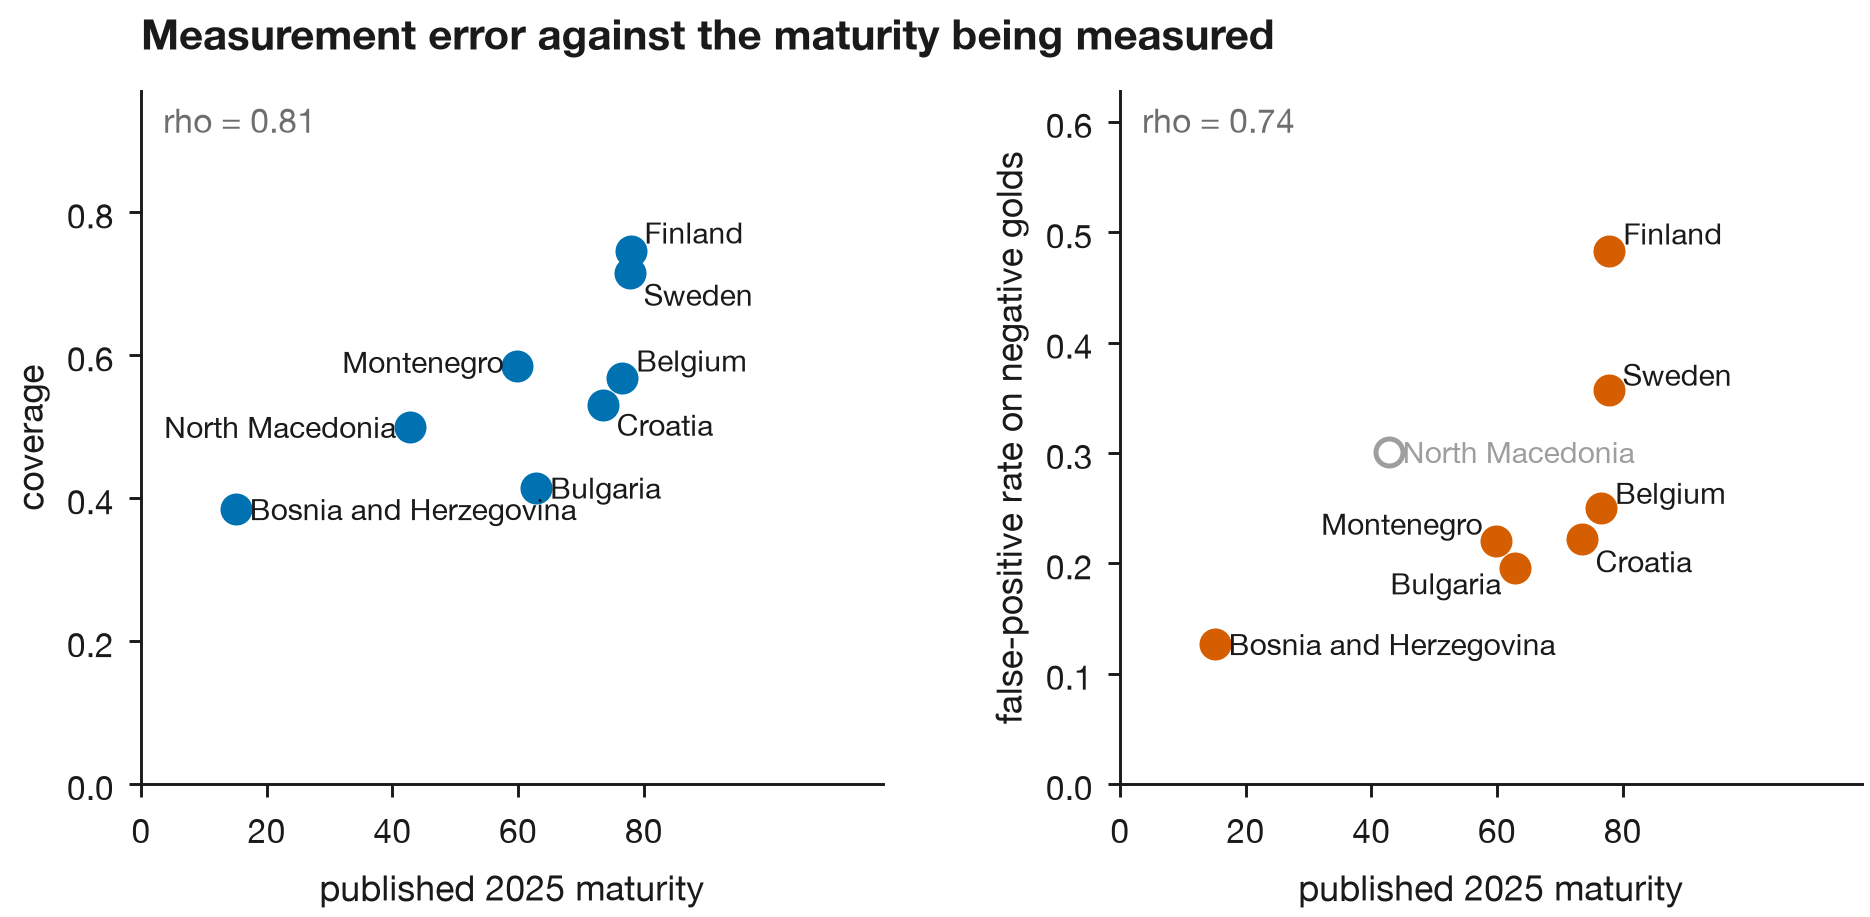
\includegraphics[width=5.9in,height=2.89321in]{media/media/image19.png}

@@CC@@Figure 5.1: Measurement error against the maturity being measured. North Macedonia, hollow, is the one country off the false-positive trend.@@/CC@@

Reproducibility confirms the same account from a third direction. Run three times over one battery with the search cache cleared between runs, the system reached the same outcome on around seven pairs in ten, and almost all of the disagreement concerned whether to answer rather than what to answer. When all three runs did commit they agreed on the label nearly every time, so the answer itself is stable and the instability sits in the decision to commit. That instability concentrates on the thin-evidence negatives whose confidence rests just above the threshold. The overall score is fairly stable, because a score pooling many questions absorbs the individual flips and commit-accuracy barely moves across the runs. The traceability condition is met for the headline run, whose logs allow every figure to be re-derived, so the part of the system that fails is judgement under thin evidence and not the discipline of the record.

Set end to end, the six verdicts@@CL@@ in Table 5.1@@/CL@@ describe one system. It is a competent retriever of positive evidence working in a setting where negative facts cannot be evidenced, and each criterion has shown a different face of this constraint. The grounded positives, the stable pooled score and the ruling-out of fabrication are what the constraint allows, while the below-baseline accuracy when forced to answer and the error that grows with the maturity being measured result from it.

@@CC@@RQ1 asked whether an automated assessment@@/CC@@ can meet the conditions that keep it legitimate, and the answer here is split. A country can see the evidence behind each answer and can see which of its questions the system declined, so the result is auditable in a way the closest comparable work is not. It cannot assume that a neighbouring country met the same standard, because the standard varies with the maturity being assessed. Automation can preserve transparency that makes an assessment challengeable, and a swarm architecture provides this where a single `black-box' agent @@CC@@cannot@@/CC@@. Yet, this does not yet preserve the even treatment that makes a ranking fair, and §5.3 sets out the change to the questionnaire that would remove that dependence.

{\def\LTcaptype{none} % do not increment counter
\begin{longtable}[]{@{}
  >{\raggedright\arraybackslash}p{(\linewidth - 8\tabcolsep) * \real{0.1635}}
  >{\raggedright\arraybackslash}p{(\linewidth - 8\tabcolsep) * \real{0.1641}}
  >{\raggedright\arraybackslash}p{(\linewidth - 8\tabcolsep) * \real{0.1111}}
  >{\raggedright\arraybackslash}p{(\linewidth - 8\tabcolsep) * \real{0.2806}}
  >{\raggedright\arraybackslash}p{(\linewidth - 8\tabcolsep) * \real{0.2806}}@{}}
\toprule\noalign{}
\begin{minipage}[b]{\linewidth}\raggedright
\textbf{Criterion}
\end{minipage} & \begin{minipage}[b]{\linewidth}\raggedright
\textbf{§2.2 condition}
\end{minipage} & \begin{minipage}[b]{\linewidth}\raggedright
\textbf{Verdict}
\end{minipage} & \begin{minipage}[b]{\linewidth}\raggedright
\textbf{Load-bearing evidence}
\end{minipage} & \begin{minipage}[b]{\linewidth}\raggedright
\textbf{Conclusion}
\end{minipage} \\
\midrule\noalign{}
\endhead
\bottomrule\noalign{}
\endlastfoot
\textbf{Convergent Validity} & Agreement with the ODMI key, and with a measure computed independently of it & Half met & Commit-accuracy 0.701 (437 of 623 scoreable committed) at coverage 0.556 (636 of 1,144). Scoring every abstention as an error, raw accuracy 0.424 (385 of 907 binary golds) against the 0.594 always-yes baseline, and balanced accuracy 0.396 against the 0.500 any single-class rule returns. Catalogue recompute against the published key, agreement on 18 of 32 measurable cells across four countries, so 44\% divergence & An automated assessment reproduces the human process on the answers it is willing to give, which is half the questionnaire. The recompute puts the answer key itself in doubt on the nine catalogue questions, so agreement with that key measures how closely the system tracks the existing process and leaves correctness open \\
\textbf{Selectivity} & Commits only where the evidence supports it, abstains otherwise, with a stated confidence that tracks observed accuracy & First condition met, second failed & Declines on 44.4\% (508 of 1,144). Aggregate ECE 0.063 over 623 scoreable committed answers, splitting to 0.089 on yes golds and 0.299 on no golds, where the sequence inverts. 86 of the 142 scoreable committed noes sit exactly at the 0.65 floor and none exceeds 0.90. Of the 88 withheld sub-floor answers carrying a no gold, 73 matched the key. & The abstention channel makes the output safe to publish, because a declined question reaches the country as a visible gap. The stated confidence carries no usable signal on the negative class, where it falls as correctness rises, so a country cannot read it as a measure of how far to trust an answer \\
\textbf{Attributability} & The quoted passage exists in the cited source, and a reasonable reader agrees it supports the claim & Settled one way, open the other & All 636 committed answers passed the offline gate, and 24 abstentions (4.7\% of 508) record an ungrounded passage against 208 (40.9\%) Verifier relevance rejections. Of the 94 negative-gold false positives, 0 of the 91 adjudicable cases vindicated the swarm & A country can contest any answer held against it, because every committed answer carries a passage present in the text the system retrieved. Whether that passage supports the label is unmeasured outside the swarm, and the false-positive audit puts the residual error there, in material that sits near the question without settling it \\
\textbf{Subgroup Equity} & Adequate performance within each subgroup, with results split by native language and maturity & Not met. The language leg came back clean and the maturity leg fails & Language leg, stratum A negative-gold false-positive rate 0.211 (55 of 261) against stratum B 0.336 (36 of 107), and committed-negative recall 0.272 against 0.178. Maturity leg, coverage, commit-accuracy and negative-gold false-positive rate all rise with published maturity at Spearman 0.81, 0.88 and 0.74 across the eight countries. Finland 0.483 (14 of 29) at maturity 77.9, Bosnia and Herzegovina 0.128 (10 of 78) at 15.1 & A ranking built from this system holds countries to different standards, because its error rises with the maturity it is trying to measure. Pooling more questions does not remove that, since an error correlated with the quantity being estimated behaves as bias and survives aggregation \\
\textbf{Generalisability} & Results decomposed by answer type and by ODMI dimension & Not met. Performance varies by dimension and collapses on the graded shapes & Commit-accuracy from 0.784 (145 of 185) on Portal to 0.622 (102 of 164) on Impact, and negative-gold false-positive rate from 0.132 (15 of 114) on Portal to 0.500 (33 of 66) on Policy. The four percentage-band questions with no catalogue route are declined on all 32 of their pairs, and the count-band questions return 1 exact match across 16 pairs. Graded questions are 19 of the 143, and 10 of 143 once the nine catalogue questions are set aside & The system can take a defined part of the questionnaire, since its accuracy follows how far the available evidence settles a question. Any published result would have to carry its per-dimension reliability, because a Policy pass and a Portal pass mean different things \\
\textbf{Reproducibility} & Traceability, a record complete enough to re-derive any reported figure. Stability, measured as variance between runs & Traceability met with one gap. Stability holds for the score and fails per question & Every Researcher, Verifier and Adjudicator call writes its prompt version, model version and raw response; the snippet picker writes no equivalent row, so its prompt and model version sit outside the record. Three replicates over the 148-pair development intersection, outcome unanimity 0.703, label agreement 0.922 (47 of 51) once all three commit, and commit-accuracy range 0.014 & The figure the ODMI would publish survives a repeat run, because the per-question flips offset each other once 143 questions pool into a score. A country reading a single answer gets a weaker guarantee, since whether the system answers that question at all moves between runs \\
\end{longtable}
}

@@CC@@Table 5.1: The six criteria of §2.2, and the verdict Chapter 4 returned on each.@@/CC@@

\section{Debate in an ODMI Environment}\label{debate-in-an-odmi-environment}

@@CC@@RQ2 asked what a swarm of distinct roles@@/CC@@ adds over a single agent, and what the adversarial stance adds in particular. The design\textquotesingle s premise was that an adversarial second agent would decorrelate the blind spots that produce an error, on the reasoning of Cohen et al. (2023) that opposition surfaces the mistakes a corroborative check misses. @@CL@@§2.5 had already qualified this, noting that decorrelation is only partial@@/CL@@ when the two agents share weights and priors. @@CC@@The ablation in §4.7 confirms it over all 1,144 evaluation pairs.@@/CC@@ Holding the architecture fixed and swapping only the Verifier\textquotesingle s stance leaves the two configurations agreeing on which pairs they get right and wrong. Of the 110 pairs exactly one arm answered correctly, 51 went to the adversarial arm and 59 to the corroborative, at a McNemar p of 0.5047. Whether a different frontier model in the Verifier\textquotesingle s role would decorrelate the errors this pairing shares is a question for future work. The results point past it, however, because the abstention gap decomposed in @@CL@@§4.4@@/CL@@ rests almost entirely on the Researcher failing to reach the confidence floor rather than on the Verifier misjudging what it retrieved. The constraint that bounds the system therefore sits on the retrieval side rather than the reasoning side, and a Verifier with stronger reasoning may be aiming at the wrong bottleneck, leaving the harder task of finding evidence untouched.

The architecture was justified by the finding of Tyen et al. (2024), that a model judges a located error far more reliably than it detects one unaided. §2 read this as the case for the Adjudicator, handing it an already-drawn disagreement to rule on, but the same finding also governs the Verifier that does the initial error pass. A positive answer can fail its evidence in two ways that are not equally locatable. In the first the passage is off-target. In the second it is on-target but insufficient. The Verifier locates the first reliably, which is most of what its relevance rejections are, and cannot locate the second, because all that separates the Researcher and Verifier is a prompt difference, which the Corroboration prompt swap-out shows has negligible effect. @@CC@@The over-read, the lower row of Figure 5.2, is therefore@@/CC@@ never surfaced as a disagreement and @@CC@@does not@@/CC@@ reach the Adjudicator.

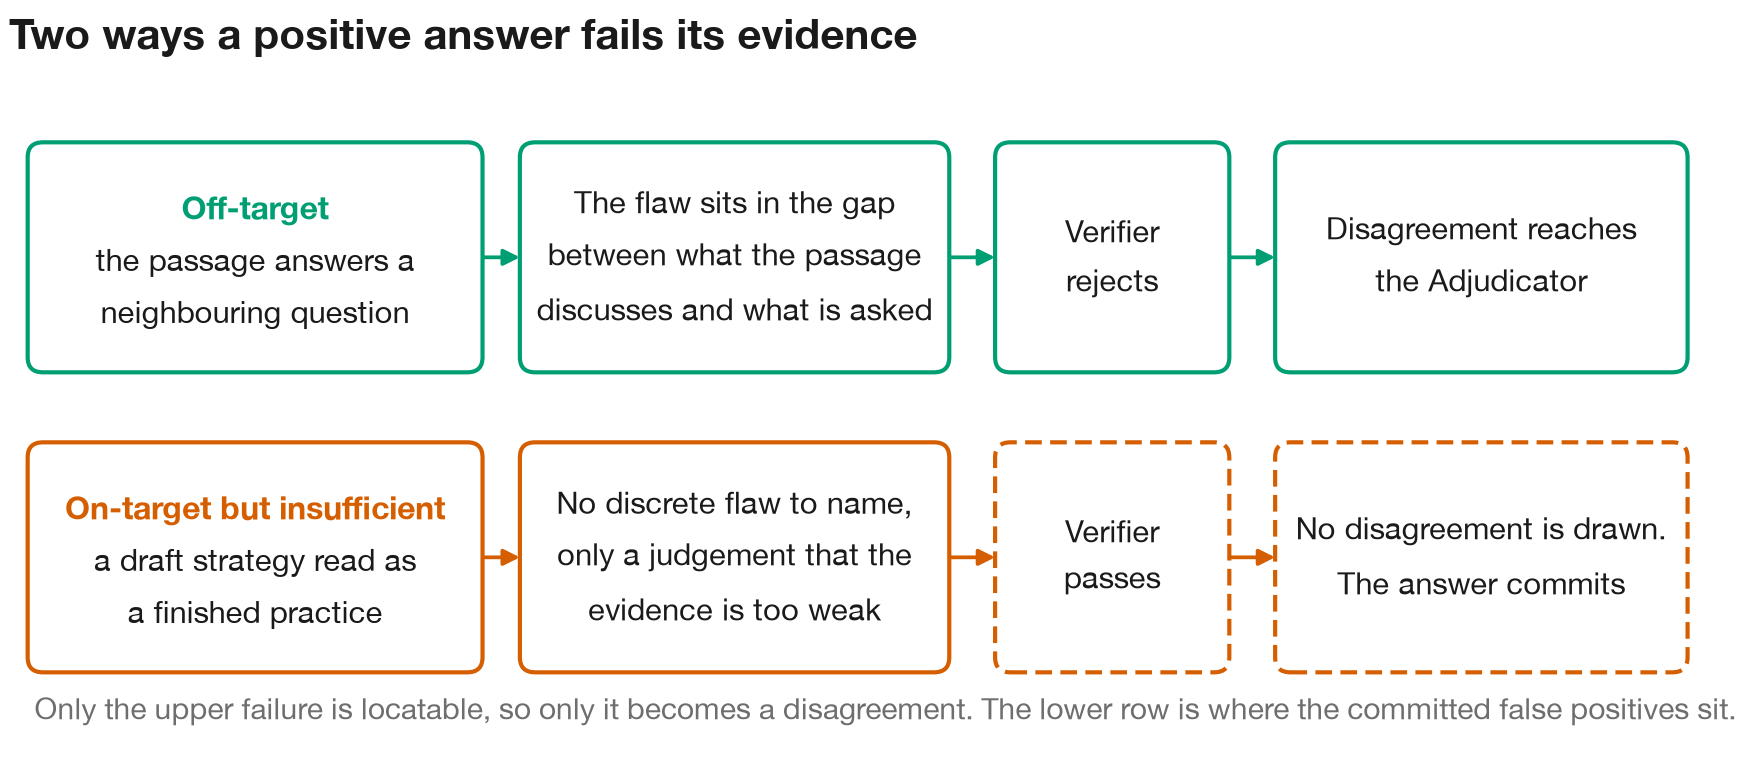
\includegraphics[width=5.9in,height=2.56287in]{media/media/image20.png}

@@CC@@Figure 5.2: Two ways a positive answer fails its evidence.@@/CC@@

The more consequential result is one none of these works anticipated. Cohen, Chowdhury and Zhu all study debate where the material to settle a claim is on hand and the open question~is how to reason over it, whereas the ODMI frequently offers evidence that is thin, adjacent or absent. The bottleneck this section has located, retrieval rather than the reasoning the debate was~built to sharpen, therefore falls outside what that literature was set up to examine, and it is where progression towards an automated assessor should be focused.

The Verifier is suited to an environment where it can set opposing evidence against the Researcher\textquotesingle s, where the answer turns on a reasoning difference over material both agents can see. The ODMI\textquotesingle s hard questions rarely provide that, since their evidence is thin, with adjacent material that reads as support for yes and nothing substantive that reads as support for no. There is little for two positions to be built from, so the debate has no practical opposition to stage. This is the setting the adversarial stance was meant for, since refuting over-reach on thin evidence is its stated purpose, yet it is the setting where it can do least. To refute a claim resting on weak but on-topic evidence the Verifier would need counterevidence the web does not hold, and without it the objection reduces to judging the evidence insufficient, a call it makes no more convincingly than the Researcher. The swarm\textquotesingle s contribution is therefore coverage, and the adversarial stance adds nothing beyond what a corroborative check already supplies.

\section{Reformulating the ODMI}\label{reformulating-the-odmi}

In their similar work, Fumega and Gao (2026) concluded that their approach still required human oversight rather than being fully autonomous. The results here extend that conclusion, since they show oversight does not have to fall evenly, as @@CC@@Figure 5.3 makes plain@@/CC@@. So, the useful question is which parts of the assessment the system can be trusted with and which have to stay manual.

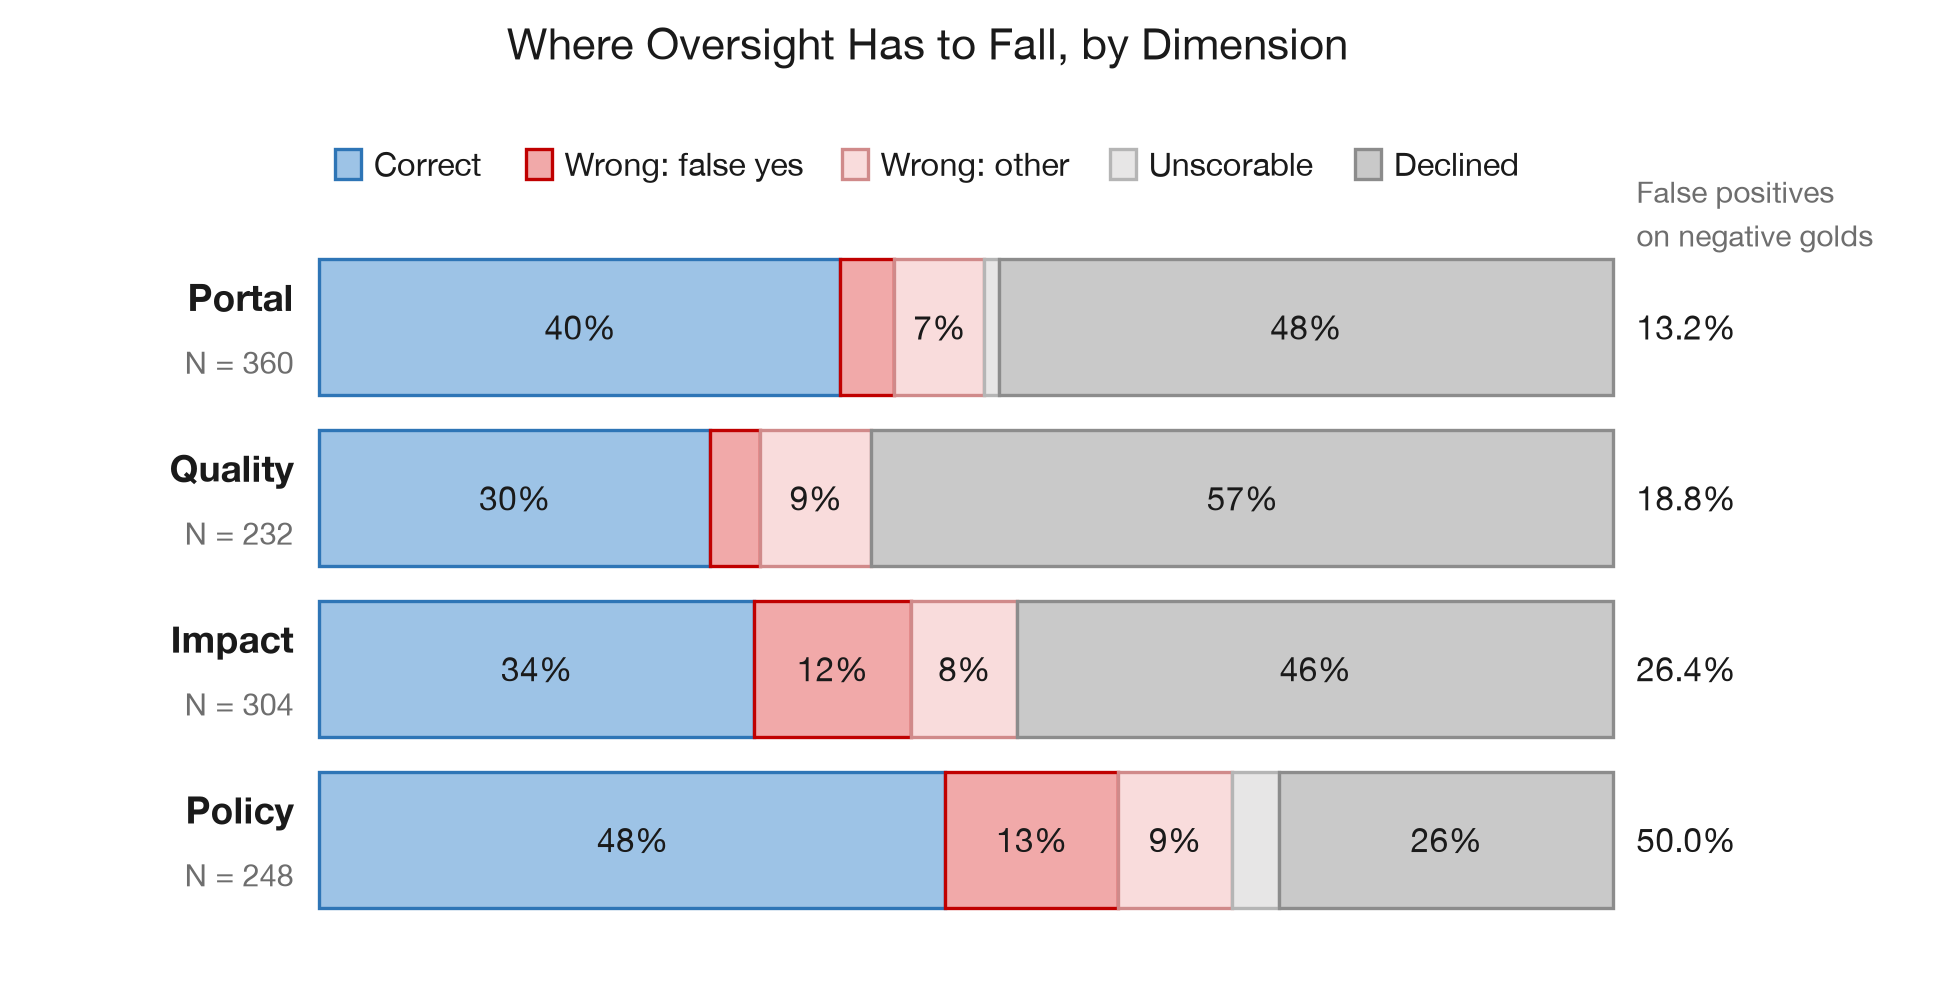
\includegraphics[width=5.89873in,height=3.01865in]{media/media/image21.png}

@@CC@@Figure 5.3: Outcome composition by ODMI dimension over the 1,144 evaluation pairs, ordered by false-positive rate on negative golds.@@/CC@@

The system is most reliable on the questions whose evidence is clear and whose nonexistence can be proved, and those are concentrated in the Portal dimension. Portal asks whether a feature is present on the national portal, which is visible on the page or absent from it, and the system commits on these at 0.784 accuracy with the lowest false-positive rate of the four dimensions. Quality behaves similarly on the questions it will answer, committing at 0.803 once its computable catalogue questions are set aside, with the second-lowest false-positive rate, though it is more cautious than Portal and declines more than half of what it is asked. Together the two are 74 of the 143 questions, the observable half of the questionnaire, the part that asks what a portal shows or a catalogue holds rather than what a team does behind it.

The catalogue questions make the case stronger still, since there the machine does not merely match the human process but appears to better it. §4.1 found the computed figure disagreeing with the recorded self-report on 44\% of the cells it could reach. The human process fills these by self-report and amends only a tenth of what countries submit, so a mechanical recount is the more trustworthy instrument on the very questions the human process is least equipped to check.

Where the process should still lie with the humans is Policy and Impact. Policy commits most readily and returns a wrong positive on half its negative questions, and the internal-practice questions spread across every dimension have little public evidence to retrieve, so both rest on internal knowledge and self-reporting that a human marker holds and the system cannot reach. These are the two operational dimensions, and leaving them to people plays to the one advantage the human process has.

The assessors meet the same limit. Across the thirty-six countries one Impact answer in eleven is "I don\textquotesingle t know", against none at all in Policy and Portal. The national teams cannot answer the dimension the swarm handles worst, so the evidence is missing for both parties. Jacobs and Wallach (2021) set out how assessments like the ODMI can diverge from what they mean to measure. They describe how there is a difference between the intangible construct, the openness of a nation's data in this case, and the tangible operationalisation, the ODMI assessment. The 143 questions stand in for that construct and approximate openness. §2.1 anticipated the shortfall, noting that automation poses a question to the assessment as much as the assessment poses one to the automation. This section takes that question up. How could the ODMI be best operationalised for a web-agent to be able to assess openness?

The reformulation this points to is not a matter of making the questions easier for a machine; it is a matter of aligning the operationalisation with the construct. A question that asks whether a team performs a practice, and accepts the team\textquotesingle s word, measures the claim about openness rather than openness itself. A question that asks for the published output of using that practice, rather than simply the existence of the practice itself, may measure openness more directly. The target of monitoring search keywords can be easily met, for example by saving a list of last month\textquotesingle s most frequent keyword terms. But setting the target of publishing the analysis of those keywords, what the team learnt from it and what they are acting on because of them, assesses the team\textquotesingle s engagement with the subject matter.

This is also the answer to the manipulation problem raised by Powers et al. (2002) and their work on automated essay scoring, where they found writers inflated an automated score more easily than they improved the actual work that was behind the score. An assessment is gameable when creating the evidence it rewards is cheaper than actually doing the activity the evidence is meant to prove@@CC@@, and the current questionnaire offers little resistance, since evidence of internal practices is largely unverifiable. @@/CC@@Requiring the published artefact reverses that for an openness index, and the current questions show the difference plainly. A country can claim to monitor its search terms at no cost, as PT28 invites, but it cannot fake having its portal\textquotesingle s source code public on GitHub, which PT43 asks for, nor a catalogue the quality assessment reads as machine-readable, which Q27 scores, without actually holding them. Where the cheapest way to satisfy a question is to produce the artefact, and the artefact is the open behaviour the question was after, scoring well on the assessment becomes a better approximation of the assessed quality.

{\def\LTcaptype{none} % do not increment counter
\begin{longtable}[]{@{}
  >{\raggedright\arraybackslash}p{(\linewidth - 6\tabcolsep) * \real{0.2836}}
  >{\raggedright\arraybackslash}p{(\linewidth - 6\tabcolsep) * \real{0.2321}}
  >{\raggedright\arraybackslash}p{(\linewidth - 6\tabcolsep) * \real{0.3116}}
  >{\raggedright\arraybackslash}p{(\linewidth - 6\tabcolsep) * \real{0.1727}}@{}}
\toprule\noalign{}
\begin{minipage}[b]{\linewidth}\raggedright
\textbf{@@CC@@Question group@@/CC@@}
\end{minipage} & \begin{minipage}[b]{\linewidth}\raggedright
\textbf{@@CC@@What it asks now@@/CC@@}
\end{minipage} & \begin{minipage}[b]{\linewidth}\raggedright
\textbf{@@CC@@What the reformed question would ask@@/CC@@}
\end{minipage} & \begin{minipage}[b]{\linewidth}\raggedright
\textbf{@@CC@@The source of evidence@@/CC@@}
\end{minipage} \\
\midrule\noalign{}
\endhead
\bottomrule\noalign{}
\endlastfoot
@@CC@@Portal features and data provision, 31 of 45@@/CC@@ & @@CC@@Whether a feature is present, with the URL already required@@/CC@@ & @@CC@@No change. Already answerable from outside@@/CC@@ & @@CC@@The live page@@/CC@@ \\
@@CC@@Portal usage and sustainability, 14 of 45@@/CC@@ & @@CC@@Whether the team monitors traffic or runs analytics@@/CC@@ & @@CC@@The published output of the monitoring, and what was acted on@@/CC@@ & @@CC@@The published report@@/CC@@ \\
@@CC@@Quality, computable from the catalogue, 9 of 29 (Q12, Q13, Q16 to Q18, Q21, Q22, Q25, Q27)@@/CC@@ & @@CC@@The team to select a percentage or count band for its own portal@@/CC@@ & @@CC@@No change to the question. Compute the figure from the harvested catalogue rather than accept the band@@/CC@@ & @@CC@@The catalogue itself@@/CC@@ \\
@@CC@@Quality, verifiable on the portal, 5 of 29 (Q5, Q8, Q11, Q15, Q19)@@/CC@@ & @@CC@@Whether a tag, standard, guideline or published page exists@@/CC@@ & @@CC@@No change. Q8 already requires the URL of the published page@@/CC@@ & @@CC@@The page, or the metadata@@/CC@@ \\
@@CC@@Quality, taken on the team\textquotesingle s word, 11 of 29 (Q1, Q3, Q4, Q6, Q7, Q9, Q10, Q14, Q20, Q23, Q24)@@/CC@@ & @@CC@@Whether the team monitors, investigates, undertakes efforts or uses a model@@/CC@@ & @@CC@@The published output of the practice: the monitoring report, the causes found, the deployment assessment@@/CC@@ & @@CC@@The published document@@/CC@@ \\
@@CC@@Policy framework, 13 of 31 (P1 to P12)@@/CC@@ & @@CC@@Whether a strategy or law contains a provision@@/CC@@ & @@CC@@Name the provision, and require the answer to quote it@@/CC@@ & @@CC@@The named clause@@/CC@@ \\
@@CC@@Policy governance, 9 of 31 (P13 to P21)@@/CC@@ & @@CC@@Whether a structure or an initiative exists@@/CC@@ & @@CC@@The share of local bodies that publish to the national portal@@/CC@@ & @@CC@@The portal\textquotesingle s publisher list@@/CC@@ \\
@@CC@@Policy implementation, 9 of 31 (P22 to P29)@@/CC@@ & @@CC@@Whether the team carries out a practice, as P28 asks for search-term monitoring@@/CC@@ & @@CC@@The published output of the practice@@/CC@@ & @@CC@@The published analysis@@/CC@@ \\
@@CC@@Impact, measuring reuse and awareness, 18 of 38@@/CC@@ & @@CC@@Whether the team measures reuse or runs awareness activities@@/CC@@ & @@CC@@The published measurement@@/CC@@ & @@CC@@The published report@@/CC@@ \\
@@CC@@Impact, reuse cases, 20 of 38@@/CC@@ & @@CC@@For a documented reuse case across four benefit areas@@/CC@@ & @@CC@@Inbound links and citations to datasets, repositories calling the portal API, dataset references in research and in the press@@/CC@@ & @@CC@@Third-party sites, outside the government estate@@/CC@@ \\
\end{longtable}
}

@@CC@@Table 5.2: What each group of questions would have to ask instead.

The demand that Policy framework questions@@/CC@@@@CL@@ in Table 5.2@@/CL@@@@CC@@ name their provision follows from @@/CC@@@@CL@@§4.5@@/CL@@@@CC@@, where the failure was over-reading an adjacent document rather than missing evidence. The governance rows ask for an outcome instead because a bare existence test is met by a nominal committee as easily as by a working one, and the monitoring rows, which run across all four dimensions, are where the reformulation is strongest.@@/CC@@

Impact resists reform more than the previous dimensions. The evidence lives outside the government websites, with an agent searching for work done by a third party that uses national data. This could live anywhere on the internet and carries no obligation to name the dataset it was built on. Dataset references in academic work and press or media use each leaves a public trace outside the government domain, and these are the least gameable evidence across the dimensions. The reformulated Impact dimension would be an independent, externally verifiable assessment of the demand side of openness.

Openness that a government enacts, whether a policy adopted, a portal feature deployed, a standard met or an analysis published, leaves a public trace, and any dimension built on it can be assessed from the outside once the question demands the trace rather than the claim. Impact leaves its trace on the sites of the people who used the data, so what it calls for is a different retrieval design as well as a different question, one that searches outward from the portal instead of inward across a government estate. All four dimensions could therefore be delegated under a reformed questionnaire. Holding the assessment to public evidence divides the questionnaire into the questions that can be externally verified and the questions taken on self-reported claims. Closing that division would not only improve the possibility of automation but would also close the gap between the construct and operationalisation of openness, because a country that publishes the analysis, the register or the conformant catalogue has demonstrated openness in the act of producing the evidence.

This is the answer to RQ3. Responsibility is not handed over whole or withheld whole but split by type of question, the machine taking what the public record can answer, and the human keeping what needs internal knowledge.@@CC@@ The observable half is the part the machine can take. In its current form, the swarm commits to about half of these questions, so a quarter of the whole questionnaire outright. It can flag the observable questions it cannot commit to, and leave the operational half wholly to the human.@@/CC@@

\section{Threats to Validity}\label{threats-to-validity}

@@CC@@Appendix A holds the full register of thirty-four modes by which the swarm can commit a wrong answer, twenty-two of them structural. The threats set out below are those bearing on the reported figures.@@/CC@@

Every retrieval finding is conditional on a single search stack. The system runs Serper and trafilatura for every query, and although the DIY pipeline laid out in §3.3 performed at least as well as the two commercial APIs it replaced, Tavily and Brave (see Experiments appendix), one implementation cannot rule out a systematic blind spot in what this combination returns. The conclusion of §5.2 is the finding most exposed to it, since holding that the binding constraint is retrieval assumes the evidence is scarce rather than that this pipeline failed to surface it.

@@CC@@Several figures rest on samples too small to estimate what they describe with precision. The replicate battery of §4.6 holds 148 pairs and the evaluation set eight countries, so confidence intervals on accuracy are wide. The ablation of §4.7 is not among them, since it runs the four arms over all 1,144 evaluation pairs and returns an equivalence on the Verifier\textquotesingle s stance at p below 0.0001, which establishes the absence of a difference instead of failing to find one. The constraint is partly the compute and search throughput available at this scale, and partly the ODMI itself, which contains thirty-six countries in total.@@/CC@@

External validity is bounded by how the evaluation set was built. Eight of the thirty-six countries were chosen to span language resource and negative-gold share rather than sampled at random, which over-represents low-resource languages and negative-rich questionnaires by design@@CC@@, a gap the always-yes baseline makes concrete at 59.4\% on these eight against 81.8\% across all thirty-six@@/CC@@, so the pooled figures do not describe the remaining twenty-eight. The extrapolation to roughly 200 hours and £1,700 for a full cycle assumes those countries behave like these eight, and the reconstructed ranking is correlated over a maturity range far wider than a real cohort spans, which makes an ordering easier to preserve than it would be across countries separated by a point or two.

The comparator is also a year out of date. The key records the 2025 cycle while the swarm read the web in 2026, so a country that adopted a policy or shipped a portal feature in the intervening year is marked wrong for answering ``yes'', and an unknown share of the committed false positives may be the swarm describing a later state of the world correctly. Testing against the 2026 key, unreleased at the time of writing, could raise the raw match rate if the average maturity continues to climb \textbf{@@CC@@as §1.2 records@@/CC@@} it doing each cycle, as there are more questions answered ``yes'' across the countries, which the system performs better on. However, the always-yes baseline would rise with it, so a higher score would not by itself show the system had improved.\textbf{@@CC@@ @@/CC@@}

Construct validity is threatened by the non-independence of the deterministic catalogue recompute, which carries the argument that the answer key cannot be fully trusted. The figures come from a single snapshot of the harvested datasets, and the Verifier repeats the same arithmetic over the same cached harvest without reaching a second source, so a divergence from the key cannot establish which of the two figures describes the portal. The one independent computation of these metrics is published by the Metadata Quality Assessment on data.europa.eu, which the leakage controls deny-list because that domain also publishes the answer key.

The language confound in @@CL@@§4.4@@/CL@@ was not resolved directly. To determine whether the higher abstention in the lower-resource stratum reflects the model's poorer reading of those languages, or simply fewer publications to read, we would need to rerun the same pairs on translated evidence, keeping the evidence constant while varying only the language the model reads. Conducting that experiment across the stratum required translation volume beyond the free tiers, so a comparison at a useful scale was not possible. Consequently, the decomposition in @@CL@@§4.4@@/CL@@ identifies the gap in the Researcher's confidence rather than in the Verifier's judgement, leaving the second branch of the question the stratification was meant to address unresolved.

\section{Legal, Social, Ethical and Professional Issues}\label{legal-social-ethical-and-professional-issues}

There are two requirements of the BCS Code of Conduct and the IET Rules of Conduct that bear directly on this work: The duty to act in the public interest and the duty to work within the limits of demonstrated competence. The first of these governs how the system collects its evidence. Every request identifies the project, the institution and a contact address. The retrieval layer reads each portal\textquotesingle s robots.txt before fetching and refuses any path the portal excludes, and where a site presents an automated challenge the fetch waits within a fixed budget and then abandons the page, so no attempt is made to defeat the check. A separate set of controls, described in §3.6, keeps the evaluation from reading ODMI\textquotesingle s own published answers. The questionnaire and the published answers it is measured against are Commission documents, reusable under Decision 2011/833/EU and released on data.europa.eu under a Creative Commons Attribution licence, so their use here carries an attribution requirement and nothing further. Evidence drawn from national portals is quoted in short passages from public pages, with the source URL recorded alongside each quotation. Model access runs through a local proxy onto a flat-rate subscription, so the costs reported in §4.8 are arithmetic equivalents computed from published per-token rates, and no figure in this report is billed spend.

§5.3 answers the second requirement, in that a system which commits to answers it cannot evidence would be worse than no system at all, and the boundary between the questions the system can be trusted with and those it cannot therefore matters more than the aggregate accuracy. What this work supports is the narrow claim that an identified subset of the assessment can be automated under stated conditions, with the remainder left to the people who carry it out now.

\chapter{Conclusion}\label{ch:conclusion}

The ODMI runs every year over 36 countries and 5,148 question-country pairs, each answer checked by hand \parencite{edp2025}, and models now are able to match humans at far lower cost on comparable text \parencite{heseltine2024,tornberg2025}. \textcite{davis2012} argue that indicators like the ODMI shape how states can be ranked and how resources will be allocated, and that the authority for this rests on contestability, where a country is able to see and dispute the evidence held against its score. Automation threatens contestability directly, because a generative assessor can produce a fluent-sounding answer without an adequate basis and the `black-box' opacity of these LLMs makes results difficult to contest. \textcite{fumega2026} ask whether AI can take over indicator evaluation without compromising contextual nuance or democratic legitimacy. The basis of evidence for responses is more important for contestability than the answers themselves, and automation needs to accommodate this.

Section~\ref{sec:criteria} assembled a novel framework for using generative models in evaluating assessments of this kind, taking inspiration from similar works for deterministic and predictive models \parencite{yung2022,williamson2012,schenk2024}. These provide a measurable way to ensure contestability: Convergent Validity, Generalisability, Subgroup Equity, Attributability, Selectivity and Reproducibility. These set out what an automated assessor has to show for its results to stay contestable. The swarm was built against them, with an adversarial Verifier to challenge each answer and an abstention channel to return nothing when the evidence is insufficient.

The swarm ran over eight countries, a total of 1,144 question-country pairs, committing an answer on 636 and declining 508, and matching the published 2025 key on 70.1\% of the committed answers that could be scored. The open-world assumption of Section~\ref{sec:open-world} governs that result. A country reporting on itself works from a complete record where silence means absence \parencite{reiter1978}, and an agent searching the open web cannot be certain. Every search returned material and no abstention came from an empty result set, so the system never fabricated evidence. What it could not do was find evidence that a practice is absent. It matched 87.0\% of the yes golds it committed on and 48.9\% of the noes, and scored 17 points lower than if it arbitrarily answered ``yes'' to each question.

Swapping the Verifier from adversarial to corroborative over the same 1,144 pairs had no significant effect on accuracy or coverage. The Researcher and the Verifier are the same Claude model separated by a prompt, and changing the prompt made no difference. What did move the result was adding calls, with the Verifier lifting coverage from 26.6\% to 46.0\% and the Adjudicator to 55.6\%, each buying answers and not precision. Current research is locating the benefit elsewhere. \textcite{chowdhury2026} assign a different model to each of their judges and put 7.5 of their 10.0-point gain on progressive evidence retrieval, and \textcite{zhu2026} attribute the benefit of debate to agent diversity. Both locate the gain somewhere other than the Verifier's stance, in fresh retrieval and in model diversity. This design retrieved fresh evidence on every retry but ran one model throughout.

Attributability, Reproducibility and Convergent Validity are mostly met. Every committed answer carried a passage found in the text the Researcher read, so the fabrication issue raised in Attributability's first condition is resolved. The Verifier is the reasonable reader the second condition asks for and halted 208 of the Researcher's claims as off-target, though an external model or human reviewer would have been a stronger test to catch the over-reads that were let through. Reproducibility holds for the most part. Receipt-taking at every step allows for easy replication of any run at any stage. The stability condition is a mixed picture. There is an insignificant 1.4 points difference in commit-accuracy over three runs, and a high 92\% agreement rate on labels it committed to, however answers near the confidence threshold were not consistent, leading to a 30\% variation on what questions were committed. For Convergent Validity, there is a 70.1\% agreement rate between the swarm's answers and the human responses. The independent recompute of deterministic questions diverged from the answer key 50\% of the time, though only four of the eight countries were computable.

Selectivity, Subgroup Equity and Generalisability all fail for the same reason. The confidence that governs the decision to answer measures how well a claim is evidenced. This works well for the positive class of answers but leaves the negative class consistently below the threshold required to commit. Selectivity fails on this directly, since its second condition asks the stated confidence be well-calibrated, and on the negative class, calibration error runs at 0.299 against 0.089 on the positive class. False positives are a consequence of this misalignment. Where little has been published about a question, a negative answer falls below the threshold and the system declines. However, where a large quantity has been published around the question, which while relevant does not directly answer the question, the material sitting near the question lifts it over the threshold and the system commits an incorrect ``yes''. The swarm declines 61.5\% of Bosnia and Herzegovina's pairs and has a false-positive rate of 12.8\% on its negative golds. For Finland, it declines 25.9\% of the questions with a false-positive rate of 48.3\%. This is Subgroup Equity failing. Furthermore, the Quality dimension has a commitment rate of 42.7\%, at an 18.8\% false-positive rate against Policy's 74.2\% and 50.0\%, which is Generalisability failing.

\textcite{jacobs2021} identify that in assessments like the ODMI, the construct of the quality of openness can diverge from its operationalisation, the assessment. In this case, a team that says it monitors its search terms will satisfy the question without actually having produced meaningful and verifiable evidence. Given this, the questionnaire in its current state could be seen to be flawed. Of the 143 ODMI questions about 20\% ask a team about its own internal practice where the supporting evidence can be seen as unverifiable. Moreover, 15.1\% of the 5,148 answers were returned with no evidence at all, and the human verifiers at Capgemini alter 10\% of answers submitted by the national teams.

There are considerable opportunities for the ODMI itself to be reformulated to address the weaknesses outlined here, so that every answer becomes publicly evidenceable. This would open far more of it to automation, as an automated assessor reading the public record doesn't rely on the self-reporting the ODMI currently depends on. This would also make the ODMI a better test of openness, because it would be searching for evidence of each country's practice rather than how they self-report, which narrows the gap between the construct of openness and the operationalisation of the assessment. The European Commission treats open data as infrastructure for wider digital policy and for artificial intelligence in particular \parencite{edp2025}. Therefore, improving the ODMI as a test of openness would enable countries to be assessed more accurately for the honesty of their practices, and any shortcomings would be reflected in their results.


% Three entries of the typed reference list are never cited in the
% prose (a docx defect carried over, flagged in the port report):
% keep them in the rendered list so it matches the typed 43.
\nocite{anthropic2026,edp2024,wei2022}
\printbibliography[heading=bibintoc, title=References]

\appendix
\chapter{Appendix}\label{appendix}

@@CL@@This appendix carries the material the body points at but has no room for, and a second group of results that did not reach Chapter 4 at all. Sections A to F support claims made in the text: the failure-mode register, the pipeline detail behind abstention and attribution, the experiment log, the questions ruled out in advance, the prior-work scoring, and the baselines. Sections G to J are new here: the full question bank, the catalogue recompute in full, the development-set results, and the figures the body does not use. Tables and figures are numbered by section, so Table C.1 is the first table of Appendix C.@@/CL@@

\section{A. Full Failure-Mode Register (FM-01 to FM-34)}\label{a.-full-failure-mode-register-fm-01-to-fm-34}

@@CL@@The register lists every way the project has identified for a wrong answer to reach the committed state. It was built by walking the pipeline stage by stage and asking what could pass each gate, not by collecting observed errors, so a mode can appear here without having fired in any run. Class is the useful column: \textquotesingle Caught\textquotesingle{} modes are stopped by a deterministic gate before commit, \textquotesingle LLM-only\textquotesingle{} modes are left as a prompt-tunable risk, and the twenty-two \textquotesingle Structural\textquotesingle{} modes cannot be closed by prompting alone. Those twenty-two are the count §5.4 cites and the attack list for further work.@@/CL@@

Severity is the product of likelihood and how silently a mode commits. `Caught' modes are stopped by a deterministic gate before commit; `LLM-only' modes are accepted as a prompt-tunable risk; `Structural' modes cannot be fixed by prompting alone @@CC@@and form the attack list for future work@@/CC@@.

{\def\LTcaptype{none} % do not increment counter
\begin{longtable}[]{@{}
  >{\raggedright\arraybackslash}p{(\linewidth - 10\tabcolsep) * \real{0.0685}}
  >{\raggedright\arraybackslash}p{(\linewidth - 10\tabcolsep) * \real{0.4302}}
  >{\raggedright\arraybackslash}p{(\linewidth - 10\tabcolsep) * \real{0.1372}}
  >{\raggedright\arraybackslash}p{(\linewidth - 10\tabcolsep) * \real{0.1274}}
  >{\raggedright\arraybackslash}p{(\linewidth - 10\tabcolsep) * \real{0.0899}}
  >{\raggedright\arraybackslash}p{(\linewidth - 10\tabcolsep) * \real{0.1469}}@{}}
\toprule\noalign{}
\begin{minipage}[b]{\linewidth}\raggedright
\textbf{ID}
\end{minipage} & \begin{minipage}[b]{\linewidth}\raggedright
\textbf{Failure mode}
\end{minipage} & \begin{minipage}[b]{\linewidth}\raggedright
\textbf{Stage}
\end{minipage} & \begin{minipage}[b]{\linewidth}\raggedright
\textbf{Class}
\end{minipage} & \begin{minipage}[b]{\linewidth}\raggedright
\textbf{Severity}
\end{minipage} & \begin{minipage}[b]{\linewidth}\raggedright
\textbf{Status}
\end{minipage} \\
\midrule\noalign{}
\endhead
\bottomrule\noalign{}
\endlastfoot
FM-01 & Quote present but does not entail the answer (relevance gap) & Verifier & LLM-only & Med & Accepted \\
FM-02 & Negating context sits outside the snippet & Evidence & Structural & High & Open \\
FM-03 & Quote proves a related but different proposition (planned≠enacted) & Verifier & LLM-only & Med & Accepted \\
FM-04 & Quote about wrong scope/entity (regional vs national) & Verifier & LLM-only & Med & Accepted \\
FM-05 & Stale evidence; no date or cycle signal supplied & Evidence & Structural & High & Open \\
FM-06 & Quantitative/band misread (82\% read as \textgreater90\%) & Verifier & LLM-only & Med & Accepted \\
FM-07 & Quote about the wrong metric & Verifier & LLM-only & Low & Accepted \\
FM-08 & Pure fabricated quote, not in any snippet & Verifier & Caught & -- & Mitigated \\
FM-09 & Snippet itself unfaithful to the live page & Evidence & Structural & High & Open \\
FM-10 & Quote--URL mismatch (quote from A, URL points to B) & Researcher & Structural & Med & Open \\
FM-11 & Substring gate false-match via loose normalisation / short quote & Deterministic & Structural & Med & Open \\
FM-12 & Cites the ODMI answer key on a listed domain/path & Deny-list & Caught & -- & Mitigated \\
FM-13 & Deny-list evasion (underscore, \%-encoding, proxy, IDN) & Deny-list & Structural & Med & Open \\
FM-14 & Third-party republication of the answer key on an allowed domain & Deny-list & Structural & High & Open \\
FM-15 & Non-authoritative source stated as fact & Verifier & LLM-only & Med & Accepted \\
FM-16 & Answer label typo / case & Deterministic & Caught & -- & Mitigated \\
FM-17 & Out-of-set answer flagged but not hard-rejected & Deterministic & Structural & Low & Open \\
FM-18 & not\_applicable chosen when the question does apply & Verifier & LLM-only & Low & Accepted \\
FM-19 & Web-unanswerable: counter-search finds nothing → pass & Verifier & Structural & High & Open \\
FM-20 & Default disprove strategy rubber-stamps (agreement bias) & Verifier & Structural & Med & Open \\
FM-21 & Correlated error: blind Verifier reaches the same wrong answer & Verifier & Structural & High & Open \\
FM-22 & Verifier confidently wrong; confidence uncalibrated & Verifier & Structural & Med & Open \\
FM-23 & Both agents agree → Adjudicator never invoked & Coordinator & Structural & High & Open \\
FM-24 & Adjudicator ratifies a plausible wrong answer & Adjudicator & LLM-only & Med & Accepted \\
FM-25 & Adjudicator overrides a valid Verifier rejection & Adjudicator & LLM-only & Med & Accepted \\
FM-26 & Commit-floor gaming: confident-wrong answer ≥0.65 & Coordinator & Structural & High & Open \\
FM-27 & Retry-until-commit within the retry budget & Coordinator & Structural & Low & Open \\
FM-28 & Stale catalogue snapshot, no age check & Catalogue & Structural & Med & Open \\
FM-29 & Partial harvest computed on an atypical sample & Catalogue & Structural & Med & Open \\
FM-30 & Zero denominator → \textless10\% band & Catalogue & Structural & Med & Open \\
FM-31 & Synthesised-conformance inflation (HU/NL/EE Q16) & Catalogue & Structural & Med & Open \\
FM-32 & Verifier recompute is the same code on the same snapshot & Catalogue & Structural & High & Open \\
FM-33 & Correlated low-resource-language error across agents & Language & Structural & Med & Open \\
FM-34 & Translation flips meaning before the model reads it & Language & Structural & Med & Open \\
\end{longtable}
}

@@CL@@Table A.1: The thirty-four failure modes by which the swarm can commit a wrong answer.@@/CL@@

\section{@@CC@@B. Pipeline Detail: Abstention Reasons, Evidence Gates and the False-Positive Audit@@/CC@@}\label{ccb.-pipeline-detail-abstention-reasons-evidence-gates-and-the-false-positive-auditcc}

@@CL@@Three parts of the pipeline are set out in full here, each of which the body states a result for without showing the workings. The first is the abstention taxonomy, which records why the swarm declined to answer on 508 of the 1,144 evaluation pairs. The second is the quote citation gate, the deterministic check that a committed answer\textquotesingle s quote really appears in the text the Researcher read, and the three ways that check is lenient. The third is the false-positive audit, the post-hoc review of every committed answer that landed against a published ``no''.@@/CL@@

\textbf{@@CL@@Why the swarm abstained@@/CL@@}

The remaining 47 sit outside that. Sixteen are fetch errors and twelve are blocked by the deny-list guarding against leakage, which makes those twelve an artefact of the evaluation protocol. The last nineteen record a mismatch inside the instrumentation, where the classifier reads the highest confidence the Researcher reached across its attempts while the commit gate reads only the last one. All nineteen have a last attempt below 0.65, and fourteen cleared every upstream gate and still ended on an Adjudicator abstention. No abstention in this run came from an empty search. The difficulty of answering the ODMI from the open web is in judging what it found.

Nine tenths of the abstentions are the system declining evidence the Researcher had retrieved, spread across four codes. The largest two are pairs whose final Verifier verdict was a rejection, 208 of them, and pairs where the Researcher never reached 0.65 on any attempt, 199. Those populations overlap heavily. Of the 208, 172 also sit below the floor, so the two codes are better read as tests applied in sequence. Of the 407 pairs they cover between them, 172 failed both, 36 the Verifier test alone and 199 the floor test alone. The Researcher declared itself inconclusive on a further 30, and the quote gate caught 24 where the cited passage could not be matched back to its source. A gold answer existed for 479 of the 508, so in most cases someone with internal access could settle a question the public web left the swarm unable to answer.

@@CC@@Codes E, G, I and D are evidence-based abstentions and account for 461 of the 508. B records an operational failure at 16, and C at 12 records the leakage guard stopping the pair before it could commit. Codes A, F1 and F3 record zero in this run.@@/CC@@

{\def\LTcaptype{none} % do not increment counter
\begin{longtable}[]{@{}
  >{\centering\arraybackslash}p{(\linewidth - 8\tabcolsep) * \real{0.0706}}
  >{\raggedright\arraybackslash}p{(\linewidth - 8\tabcolsep) * \real{0.5941}}
  >{\centering\arraybackslash}p{(\linewidth - 8\tabcolsep) * \real{0.0882}}
  >{\centering\arraybackslash}p{(\linewidth - 8\tabcolsep) * \real{0.0882}}
  >{\centering\arraybackslash}p{(\linewidth - 8\tabcolsep) * \real{0.1588}}@{}}
\toprule\noalign{}
\begin{minipage}[b]{\linewidth}\centering
\textbf{Code}
\end{minipage} & \begin{minipage}[b]{\linewidth}\raggedright
\textbf{Reason}
\end{minipage} & \begin{minipage}[b]{\linewidth}\centering
\textbf{n}
\end{minipage} & \begin{minipage}[b]{\linewidth}\centering
\textbf{\%}
\end{minipage} & \begin{minipage}[b]{\linewidth}\centering
\textbf{Gold existed}
\end{minipage} \\
\midrule\noalign{}
\endhead
\bottomrule\noalign{}
\endlastfoot
E & Verifier relevance rejection & @@CC@@208@@/CC@@ & @@CC@@41\%@@/CC@@ & @@CL@@202 of 208@@/CL@@ \\
G & Below the 0.65 confidence floor & @@CC@@199@@/CC@@ & @@CC@@39\%@@/CC@@ & @@CL@@182 of 199@@/CL@@ \\
I & Researcher never committed (said inconclusive itself) & @@CC@@30@@/CC@@ & @@CC@@6\%@@/CC@@ & @@CL@@30 of 30@@/CL@@ \\
D & Evidence ungrounded (substring/quote gate failed) & @@CC@@24@@/CC@@ & @@CC@@5\%@@/CC@@ & @@CL@@21 of 24@@/CL@@ \\
B & Fetch error (4xx/5xx/timeout) & @@CC@@16@@/CC@@ & @@CC@@3\%@@/CC@@ & @@CL@@16 of 16@@/CL@@ \\
A & Thin web / no search results & @@CC@@0@@/CC@@ & @@CC@@0\%@@/CC@@ & @@CL@@--@@/CL@@ \\
F3 & Search-empty hard failure & @@CC@@0@@/CC@@ & @@CC@@0\%@@/CC@@ & n/a \\
C & Deny-listed / MQA source (leakage guard) & @@CC@@12@@/CC@@ & @@CC@@2\%@@/CC@@ & @@CL@@12 of 12@@/CL@@ \\
F1 & Schema-invalid hard failure & @@CC@@0@@/CC@@ & @@CC@@0\%@@/CC@@ & n/a \\
Z & @@CL@@Instrumentation mismatch: the classifier reads peak confidence, the commit gate reads the last attempt (§4.2)@@/CL@@ & @@CC@@19@@/CC@@ & @@CC@@4\%@@/CC@@ & @@CL@@16 of 19@@/CL@@ \\
& \textbf{Total (all no-commits)} & \textbf{@@CC@@508@@/CC@@} & \textbf{100\%} & @@CL@@479 of 508@@/CL@@ \\
\end{longtable}
}

@@CL@@Table B.1: Why the swarm did not commit, over the 508 evaluation abstentions.@@/CL@@

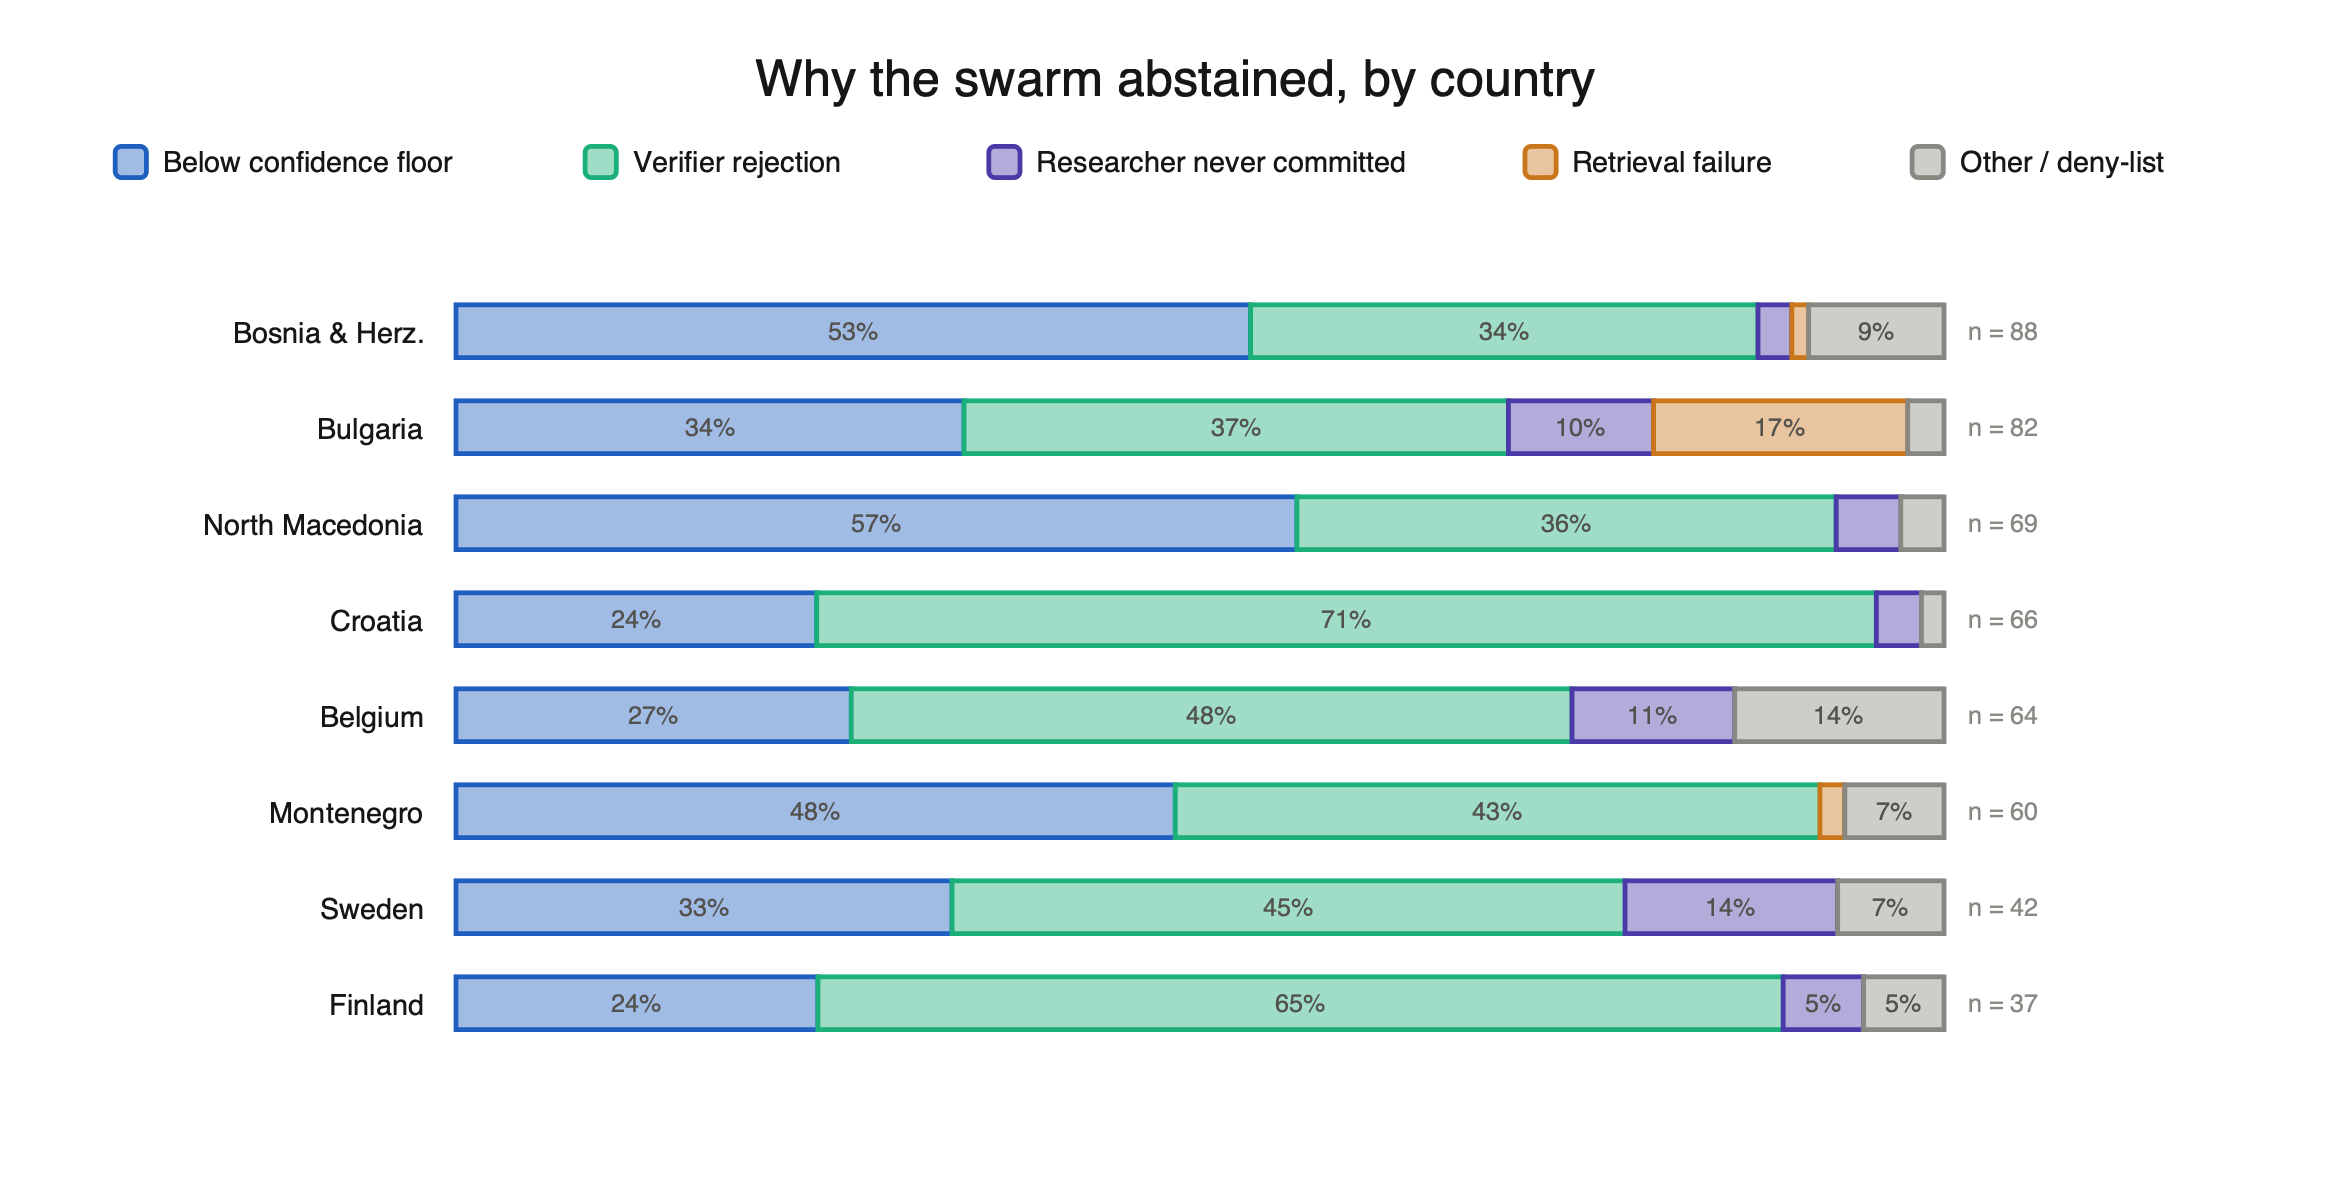
\includegraphics[width=6.1in,height=3.06297in]{media/media/image22.png}

@@CL@@Figure B.1: Why the swarm abstained, by country. The 508 evaluation abstentions grouped into five causes.@@/CL@@

\textbf{@@CL@@The quote citation gate, Attributability part 1@@/CL@@}

The gate is deliberately lenient, however, in three recorded ways. The comparison normalises Unicode and case, strips punctuation and collapses whitespace, and sets no minimum quote length, so a two- or three-word string or a light paraphrase satisfies it. The cited URL is checked only for membership of the result set, with nothing binding a quote to the page it was read on, so a passage from one page can be filed against another. Nothing compares the retrieved snippet against the live page, so where the picker has paraphrased, the gate certifies the paraphrase. The normalisation is deliberate as an exact byte comparison fails on encoding differences, smart quotes and whitespace artefacts that are not misquotes, and would discard correct answers. Quality assurance is the price of this.~So the worst case the gate lets through is a committed answer whose quote is real but thin, a handful of genuine words, or a paraphrase of them, that a reader would not accept as settling the question. It holds against fabrication and hands misattribution to the Verifier.

\textbf{@@CL@@The false-positive audit@@/CL@@}

@@CL@@Every committed answer that disagrees with a published ``no'' is a false positive, and the evaluation run produced 94 of them. The audit exists because a disagreement is not automatically a swarm error: the published answer is a country\textquotesingle s own self-report and can be a cycle out of date, so the question is whether the swarm over-read its evidence or found something the assessors missed. Each case was put to a separate reviewer, claude-opus-4-6, with the swarm\textquotesingle s own cited passage and the ODMI\textquotesingle s published explanation in front of it. 91 of the 94 are committed yes answers and were adjudicated; the remaining three, MK I4, Q5 and Q6, answer not applicable against a no gold, which the yes-defending rubric cannot score, so they are flagged for manual review rather than judged.@@/CL@@

The first framing is neutral. The reviewer is shown the ODMI gold answer and its published explanation and asked to account for the disagreement, with the prompt stating it must be ``strict and concrete''. Is this a genuine error, where the swarm misread evidence a reader would have rejected? A definitional gap, where the swarm answered a slightly different question than the one the ODMI scored? Or a defensible answer against a gold that may itself be stale or self-reported? The pass sorts the false positives by why they went wrong.

The second framing is pro-swarm. The reviewer is instructed to act as an advocate for swarm, being asked to build the ``strongest possible evidence-grounded case'' that the swarm\textquotesingle s ``yes'' was right and the ODMI\textquotesingle s ``no'' was mistaken, and to return one of three verdicts: that the swarm over-read its evidence even on the most generous reading, that the case is ambiguous, or that the gold is wrong and the swarm is vindicated. This is the stringent test. A false positive counts as the swarm being right only if a reviewer actively trying to prove that, from the evidence the swarm itself cited, can succeed.

{\def\LTcaptype{none} % do not increment counter
\begin{longtable}[]{@{}
  >{\raggedright\arraybackslash}p{(\linewidth - 6\tabcolsep) * \real{0.1671}}
  >{\raggedright\arraybackslash}p{(\linewidth - 6\tabcolsep) * \real{0.5504}}
  >{\raggedright\arraybackslash}p{(\linewidth - 6\tabcolsep) * \real{0.0688}}
  >{\raggedright\arraybackslash}p{(\linewidth - 6\tabcolsep) * \real{0.0885}}@{}}
\toprule\noalign{}
\begin{minipage}[b]{\linewidth}\raggedright
\textbf{@@CL@@Pass@@/CL@@}
\end{minipage} & \begin{minipage}[b]{\linewidth}\raggedright
\textbf{@@CL@@Verdict@@/CL@@}
\end{minipage} & \begin{minipage}[b]{\linewidth}\raggedright
\textbf{@@CL@@n@@/CL@@}
\end{minipage} & \begin{minipage}[b]{\linewidth}\raggedright
\textbf{@@CL@@Share@@/CL@@}
\end{minipage} \\
\midrule\noalign{}
\endhead
\bottomrule\noalign{}
\endlastfoot
@@CL@@Pass 1, charitable@@/CL@@ & @@CL@@Genuine error, the swarm misread evidence a reader would have rejected@@/CL@@ & @@CL@@16@@/CL@@ & @@CL@@18\%@@/CL@@ \\
& @@CL@@Definitional gap, the swarm answered a slightly different question@@/CL@@ & @@CL@@69@@/CL@@ & @@CL@@76\%@@/CL@@ \\
& @@CL@@Defensible, or the gold may be stale@@/CL@@ & @@CL@@6@@/CL@@ & @@CL@@7\%@@/CL@@ \\
@@CL@@Pass 2, advocate@@/CL@@ & @@CL@@Swarm over-read its evidence even on the most generous reading@@/CL@@ & @@CL@@68@@/CL@@ & @@CL@@75\%@@/CL@@ \\
& @@CL@@Ambiguous@@/CL@@ & @@CL@@23@@/CL@@ & @@CL@@25\%@@/CL@@ \\
& @@CL@@Gold wrong, swarm vindicated@@/CL@@ & @@CL@@0@@/CL@@ & @@CL@@0\%@@/CL@@ \\
\end{longtable}
}

@@CL@@Table B.2: The false-positive audit, over the 91 adjudicated cases of the 94. Shares are of 91.

The two passes agree on the direction. Nothing in the audit supports the swarm against the published key: the advocate pass returns ``no'' case at all where the gold is wrong and the swarm right. That is what licenses treating match against ODMI as a fair measure rather than one inflated by stale ground truth, and it is the basis for the staleness band §3.4 discusses being treated as negligible.@@/CL@@

\section{@@CC@@C. Experiments@@/CC@@}\label{ccc.-experimentscc}

@@CL@@Every experiment was registered before dispatch, in a design note fixing the question, the sample, the endpoint and the adoption rule, and in a machine-readable row carrying the same design. The table below is that register, filtered to the runs that completed. The paragraph after it is the model comparison, reproduced from §4.8 because the numbers behind it live in this appendix rather than in the body.@@/CL@@

\textbf{@@CL@@The completed experiments@@/CL@@}

\textbf{@@CL@@Model choice@@/CL@@}

Another lever on this cost is the choice of model, which sets both the reasoning model and the model that picks the snippets. Comparing models from the same family on the same 156 development-set pairs, Haiku 4.5 delivered 28.8\% accuracy, Sonnet 4.6 delivered 34.0\% at 1.4 times Haiku\textquotesingle s cost per correct answer, and Opus 4.8 delivered 21.8\% at 4.6 times. Opus is dominated on both axes, being the least accurate and the most expensive of the three. Coverage explains the ordering. Haiku committed to 43\% of the battery, Sonnet to 46.8\% and Opus to 29.5\%, and total accuracy counts an abstention as a failure. On committed answers alone the three converge, at 67.2\% for Haiku, 72.6\% for Sonnet and 73.9\% for Opus. With this lens Opus is not worse at answering these questions, it is more reluctant to answer them, and marginally the most accurate when it does. Like the Verifier stance in @@CL@@§4.7@@/CL@@, changing the model moves how much the system is willing to say rather than how often it is right. Sonnet is retained because it commits most, at a middling price, with commit-accuracy indistinguishable from a model costing over three times as much.

Completed experiments:

{\def\LTcaptype{none} % do not increment counter
\begin{longtable}[]{@{}
  >{\raggedright\arraybackslash}p{(\linewidth - 8\tabcolsep) * \real{0.1106}}
  >{\raggedright\arraybackslash}p{(\linewidth - 8\tabcolsep) * \real{0.2295}}
  >{\raggedright\arraybackslash}p{(\linewidth - 8\tabcolsep) * \real{0.2428}}
  >{\raggedright\arraybackslash}p{(\linewidth - 8\tabcolsep) * \real{0.2362}}
  >{\raggedright\arraybackslash}p{(\linewidth - 8\tabcolsep) * \real{0.1808}}@{}}
\toprule\noalign{}
\begin{minipage}[b]{\linewidth}\raggedright
\textbf{Exp}
\end{minipage} & \begin{minipage}[b]{\linewidth}\raggedright
\textbf{Experiment}
\end{minipage} & \begin{minipage}[b]{\linewidth}\raggedright
\textbf{Scope (n)}
\end{minipage} & \begin{minipage}[b]{\linewidth}\raggedright
\textbf{Result}
\end{minipage} & \begin{minipage}[b]{\linewidth}\raggedright
\textbf{Outcome}
\end{minipage} \\
\midrule\noalign{}
\endhead
\bottomrule\noalign{}
\endlastfoot
EXP-1 & Search provider: DIY vs Tavily & France, 90 pairs (55 decided) & DIY at least as good on 89\% of decided pairs (Wilson 78-95), leads all three dimensions & DIY adopted \\
EXP-17 & Snippet picker on vs off & Netherlands, n=50 & Recall unchanged; removing it raised cost \textasciitilde57\% and cut coverage & Keep the picker \\
EXP-17, EXP-18 & Retrieval breadth (5 vs 10 results) & Netherlands n=50; multi-country FR+AL+NL & The r10 gain rested on a single NL run at +17\% cost and never confirmed multi-country & Keep 5 results per query \\
EXP-24 & Snippet truncation cap & Netherlands replay, 25 abstained pairs & 3,000-char cap committed 15 vs 12 with no gain in correct answers and three abstain-to-wrong flips & Keep 600 \\
EXP-34 & Trusted-domain narrow-then-widen retrieval & NL+MT+AL, 156-pair dev battery & @@CC@@Clean null: pooled false-positive McNemar p = 0.727, paired accuracy an exact tie@@/CC@@ & @@CC@@No detectable difference@@/CC@@ \\
EXP-11 & Verifier redesign (tristate / gated) & Dev ladder, 150 frozen candidates & Incumbent disprove J = 0.41 against tristate 0.03 and the deterministic gate 0.02 & Retain incumbent \\
EXP-12 & Verifier evidence ladder & Dev + Malta / Norway & Counter-search helps no-claims, hurts yes-claims & Informs D45 \\
EXP-38 & Corroborative vs adversarial verifier framing & 150 frozen candidates, search-free replay & Disprove J = 0.41 against corroborate J = 0.16 via a sensitivity collapse 0.72 to 0.32; adversarialism costs twice the false-rejection rate & Adversarial framing retained; the trade reported \\
EXP-13a & Value of the verify-and-adjudicate layer & Malta 60 + Norway 143 & Removing it costs 27 correct and adds 43 abstentions & Keep the layer \\
EXP-14 & Verifier counter-search (never vs always) & Netherlands, n=51 & No significant difference (McNemar p = 0.50); \textquotesingle never\textquotesingle{} raises false positives & Keep \textquotesingle always\textquotesingle{} \\
EXP-19 & Verifier counter-search, multi-country & NL+MT+AL, \textasciitilde78 negative golds & Pooled marginal favours \textquotesingle never\textquotesingle{} but is composition-confounded; paired McNemar null (p = 1.00) & Keep \textquotesingle always\textquotesingle{} \\
EXP-16 & Adjudicator free vs standard selection & Netherlands, n=51 & No difference (p = 1.00) & Keep \textquotesingle standard\textquotesingle{} \\
EXP-7 & Retry chaining (carry evidence across retries) & Malta, 40 per arm & Small, underpowered gain; joint non-inferiority passes & Adopt as optimisation baseline \\
EXP-20 & Retry chaining on committing countries & NL+AL & Balanced accuracy rises but false-positive rate rose 0.346 to 0.387; McNemar p = 0.500 & Keep baseline; not promoted \\
EXP-10 & Confidence-floor sweep & Pooled, 7 countries, n=360, 67 negative golds & 0.65 holds; at 0.50 precision is 0.76, under the pre-registered 0.80 bar & Floor 0.65 \\
EXP-25, EXP-27 & Commit gates (entailment, argue-the-opposite) & Netherlands, n=50, 25 negative golds & Null and harmful; both raise the negative-gold false-positive rate & The 0.65 floor remains the precision control \\
EXP-22 & Foreign-language query ablation & Albania & Null: suppressing the native-language query changed nothing & Keep bilingual queries \\
EXP-39 & Language-comprehension probes (no DeepL) & Frozen 150 subset, local OPUS-MT & Part A null after the mandated translation-quality gate; third independent language null & No comprehension penalty demonstrated \\
EXP-32 & All-Haiku whole-stack cost point & 156-pair dev battery & Lower anchor of the cost-quality frontier & Frontier point, not adopted \\
EXP-41 & Run-to-run stability & 3 replicates, 148-pair intersection & Label agreement 0.922, three-way unanimity 0.703, evidence-path divergence 0.894 & Answers stable, evidence paths are not \\
EXP-36 & Frozen headline whole-system run & Evaluation 8, 1,144 pairs & Coverage 0.556, commit-accuracy 0.701 {[}0.664, 0.736{]}, negative-gold FPR 0.247, ECE 0.063 & The reported headline \\
EXP-28 & Architecture ablation ladder (researcher only / no adjudicator / trio). Sonnet 5, superseded by Table 4.7.1 & 156-pair dev battery, 78 negative golds & Commit rate 0.237, 0.391, 0.468 and commit-accuracy 0.649, 0.689, 0.726 across the three arms; negative-gold false-positive rate rises 0.13 to 0.22 (ten wrong to seventeen of 78) & Each layer adds coverage and accuracy; the Verifier does not filter for precision \\
EXP-40 & Corroborative vs adversarial verifier, end to end & 156-pair dev battery & Balanced accuracy 0.261 against 0.262; sixteen discordant pairs split eight-eight; McNemar p = 1.00 & Null end to end, against the EXP-38 frozen-ladder result \\
@@CC@@exp36\_model\_opus@@/CC@@ & @@CC@@All-Opus whole-stack cost point@@/CC@@ & @@CC@@156-pair dev battery@@/CC@@ & @@CC@@Delivered accuracy 21.8\% at £22.12, £0.65 per correct answer; worse than Sonnet 4.6 (p \textless{} 0.001) and Haiku 4.5 (p = 0.035)@@/CC@@ & @@CC@@Upper anchor of the cost-quality frontier; dominated on both axes, not adopted@@/CC@@ \\
@@CC@@cb\_heldout\_20260725@@/CC@@ & @@CC@@Closed-book parametric probe (retrieval disabled)@@/CC@@ & @@CC@@Evaluation 8, 1,144 pairs@@/CC@@ & @@CC@@42.9\% of the answer key reproduced against the 47.3\% always-yes floor@@/CC@@ & @@CC@@Below the floor; no answer-key memorisation demonstrated@@/CC@@ \\
@@CC@@heldout\_fp\_audit\_merged94@@/CC@@ & @@CC@@False-positive audit of the evaluation negative-gold errors@@/CC@@ & @@CC@@94 EXP-36 false positives, 91 adjudicable@@/CC@@ & @@CC@@Charitable pass: 16/91 genuine swarm error, 69/91 definitional gap, 6/91 defensible or stale gold. Adversarial pass: 0/91 gold wrong@@/CC@@ & @@CC@@No case of the swarm right and ODMI wrong; the 3 not\_applicable pairs flagged for manual review@@/CC@@ \\
\end{longtable}
}

@@CL@@Table C.1: The completed experiments, with the sample, result and adoption rule for each.@@/CL@@

\textbf{@@CL@@What the orchestrator refuses@@/CL@@}

@@CC@@The orchestrator refuses to dispatch a run where the experiment identifier has no row in the registry, where two arms differ from the baseline in more than one setting, where a specification names an evaluation country, where two arms share an identifier, or where no ceiling has been declared on the number of model calls the run may spend. Each is a hard failure that halts the run before any expenditure.@@/CC@@

\section{D. Out-of-Reach Questions}\label{d.-out-of-reach-questions}

@@CC@@The 29 questions judged systematically out of reach of a web agent. The rule is that the answer is a fact about internal operational behaviour for which there is no standard public artefact. Questions answerable from a policy document, observable as a portal feature, computable from harvested metadata, or which themselves ask whether something is published, are excluded. The classification was made from the question text alone, before any run data was consulted.@@/CC@@

{\def\LTcaptype{none} % do not increment counter
\begin{longtable}[]{@{}
  >{\raggedright\arraybackslash}p{(\linewidth - 2\tabcolsep) * \real{0.1386}}
  >{\raggedright\arraybackslash}p{(\linewidth - 2\tabcolsep) * \real{0.8614}}@{}}
\toprule\noalign{}
\begin{minipage}[b]{\linewidth}\raggedright
\textbf{Question}
\end{minipage} & \begin{minipage}[b]{\linewidth}\raggedright
\textbf{Text}
\end{minipage} \\
\midrule\noalign{}
\endhead
\bottomrule\noalign{}
\endlastfoot
P18 & Is there a regular exchange of knowledge or experiences between the national open data team and the team maintaining the national portal? \\
P20 & Is there a regular exchange of knowledge or experiences between the national open data team and the wider network of open data officers in your country? \\
P25 & Are there any processes in place to assess if public sector bodies are charging for data above marginal cost? (please see directive (EU) 2019/1024 on open data and the reuse of public sector information). \\
PT15 & Does the team monitor the extent to which requests (either via the portal or otherwise) result in the publication of the requested data? \\
PT23 & Do you monitor the portal\textquotesingle s traffic (e.g. in terms of number of unique visitors, visitor profiles, percentage of machine traffic, number of downloads according to the number of datasets etc.)? \\
PT24 & Do you run analytics on API usage? \\
PT25 & Besides monitoring portal traffic, do you perform any further activities to better understand the behaviour and needs of users of your portal (e.g. web analytics, surveys, or analysis of social media feeds)? \\
PT26 & Do you use the insights about portal usage and about the behaviour and needs of portal users to improve the portal accordingly? \\
PT28 & Do you monitor what keywords are used to search for data and content on the portal? \\
PT29 & Do you monitor the most and least consulted pages? \\
PT33 & Do you identify the data providers that are not yet publishing data on the national portal? \\
PT34 & Were there concrete actions taken to assist these data providers with their publication process? \\
PT44 & Do you monitor the characteristics of the data published on the portal, such as the distribution across categories, static vs. real-time data and how these change over time? \\
PT45 & Does this monitoring enable the portal team and/or data providers to take action to improve their performance on the national portal? \\
Q1 & Is there a pre-defined approach to ensure that metadata is kept up-to-date? \\
Q4 & Do you undertake efforts to ensure that published data covers the full period from when it was first published until today, for example, the complete time series? \\
Q7 & Do you monitor the quality of the metadata available on your portal? \\
Q20 & Do you investigate the most common causes for the lack of DCAT-AP compliance? \\
I4 & Does your country have processes in place to monitor and measure the level of reuse of high-value datasets ((EU) 2023/138)? \\
I8 & Have any public bodies in your country launched or performed any activities in the past year to understand which and how (open) datasets are reused? \\
I8-a & Automated feedback mechanisms tracking users´ access to datasets \\
I8-b & Surveys \\
I8-c & Interviews/workshops with reusers \\
I8-d & Other \\
I9 & Have any public bodies in your country launched or performed any activities in the past year to better understand reusers\textquotesingle{} needs in order to further stimulate the reuse of open data? \\
I9-a & Regular feedback sessions with portal users \\
I9-b & Social media sentiment analysis \\
I9-c & Other \\
I11 & Are there any public bodies in your country that have developed a systematic ways of classifying the gathered reuse cases? \\
\end{longtable}
}

@@CL@@Table D.1: The 29 questions judged out of reach of a web agent.@@/CL@@

\section{@@CC@@E. Prior Work Scored Against the Six Criteria, with Justifications@@/CC@@}\label{cce.-prior-work-scored-against-the-six-criteria-with-justificationscc}

@@CC@@The abridged version of this table@@/CC@@@@CL@@, Table E.1,@@/CL@@@@CC@@ appears as Table 2.2@@/CC@@@@CL@@ in §2.8@@/CL@@@@CC@@. Verdicts are read from the papers themselves, and quoted passages are taken verbatim from the primary text. A tick means the work addresses and reports the criterion, not that it succeeds. Partial means it addresses one of the criterion's two conditions, or reports it without measuring it.@@/CC@@

{\def\LTcaptype{none} % do not increment counter
\begin{longtable}[]{@{}
  >{\raggedright\arraybackslash}p{(\linewidth - 12\tabcolsep) * \real{0.1427}}
  >{\raggedright\arraybackslash}p{(\linewidth - 12\tabcolsep) * \real{0.1428}}
  >{\raggedright\arraybackslash}p{(\linewidth - 12\tabcolsep) * \real{0.1429}}
  >{\raggedright\arraybackslash}p{(\linewidth - 12\tabcolsep) * \real{0.1427}}
  >{\raggedright\arraybackslash}p{(\linewidth - 12\tabcolsep) * \real{0.1428}}
  >{\raggedright\arraybackslash}p{(\linewidth - 12\tabcolsep) * \real{0.1430}}
  >{\raggedright\arraybackslash}p{(\linewidth - 12\tabcolsep) * \real{0.1429}}@{}}
\toprule\noalign{}
\begin{minipage}[b]{\linewidth}\raggedright
@@CC@@Work@@/CC@@
\end{minipage} & \begin{minipage}[b]{\linewidth}\raggedright
@@CC@@Convergent Validity@@/CC@@
\end{minipage} & \begin{minipage}[b]{\linewidth}\raggedright
@@CC@@Generalisability@@/CC@@
\end{minipage} & \begin{minipage}[b]{\linewidth}\raggedright
@@CC@@Subgroup Equity@@/CC@@
\end{minipage} & \begin{minipage}[b]{\linewidth}\raggedright
@@CC@@Attributability@@/CC@@
\end{minipage} & \begin{minipage}[b]{\linewidth}\raggedright
@@CC@@Selectivity@@/CC@@
\end{minipage} & \begin{minipage}[b]{\linewidth}\raggedright
@@CC@@Reproducibility@@/CC@@
\end{minipage} \\
\midrule\noalign{}
\endhead
\bottomrule\noalign{}
\endlastfoot
@@CC@@ReAct (Yao et al., 2023)@@/CC@@ & @@CC@@Reports accuracy on HotpotQA and Fever and success-rate gains of 34\% and 10\% on ALFWorld and WebShop, against task gold rather than a human assessor key.@@/CC@@ & @@CC@@Four benchmarks over two families, question answering and interactive decision making.@@/CC@@ & @@CC@@Not addressed.@@/CC@@ & @@CC@@Retrieves through "a simple Wikipedia API" and leaves trajectories "more interpretable than baselines without reasoning traces". No check that a quoted passage exists in the source.@@/CC@@ & @@CC@@No abstention and no confidence output.@@/CC@@ & @@CC@@"All methods use greedy decoding" and prompts are published. No repeated runs and no variance.@@/CC@@ \\
@@CC@@SelfCheckGPT (Manakul et al., 2023)@@/CC@@ & @@CC@@AUC-PR against manual factuality annotation. No agreement percentage reported.@@/CC@@ & @@CC@@WikiBio only, with synthetically generated hallucinations.@@/CC@@ & @@CC@@Not addressed.@@/CC@@ & @@CC@@Zero-resource by design. External knowledge appears only as an ablation showing what could be done instead.@@/CC@@ & @@CC@@Produces a per-sentence hallucination score that could drive a gate, but never declines and reports no calibration.@@/CC@@ & @@CC@@Main response at "temperature to 0.0 and standard beam search decoding". Sampling is internal to the method and is not a stability measure.@@/CC@@ \\
@@CC@@Chain-of-Verification (Dhuliawala et al., 2024)@@/CC@@ & @@CC@@Reports hallucination reduction across tasks with no single headline agreement figure.@@/CC@@ & @@CC@@Three task types, Wikidata list questions, closed-book MultiSpanQA and long-form generation.@@/CC@@ & @@CC@@Not addressed.@@/CC@@ & @@CC@@Tool-free by design. Retrieval appears only as related work.@@/CC@@ & @@CC@@No abstention and no confidence. Confidence scoring is attributed to Varshney et al., not to CoVe.@@/CC@@ & @@CC@@"Use greedy decoding for all models". No repeated runs.@@/CC@@ \\
@@CC@@LM vs LM (Cohen et al., 2023)@@/CC@@ & @@CC@@"Detects over 70\% of the incorrect claims while maintaining a high precision".@@/CC@@ & @@CC@@Four benchmarks.@@/CC@@ & @@CC@@Not addressed.@@/CC@@ & @@CC@@"We are not assuming any reference text or an external knowledge base." The examiner asks whether external evidence exists without ever retrieving any.@@/CC@@ & @@CC@@Frames its setting as related to calibration and abstention, but outputs a decision and never declines.@@/CC@@ & @@CC@@Applies the method "three times (with the same EXAMINER and EXAMINEE), using sampling" for the majority variant.@@/CC@@ \\
@@CC@@Du et al. (2023)@@/CC@@ & @@CC@@Accuracy across six benchmarks against task gold.@@/CC@@ & @@CC@@Six benchmarks including mathematics, MMLU and chess move validity.@@/CC@@ & @@CC@@Not addressed.@@/CC@@ & @@CC@@Retrieval is described as orthogonal to the method and is not used.@@/CC@@ & @@CC@@Observes that uncertain facts diverge across agents, but provides no abstention channel.@@/CC@@ & @@CC@@Reports standard deviations throughout, for example "Single Agent 67.0 ± 4.7" and "Multi-Agent (Majority) 69.0 ± 4.6", with identical prompt and model across arms.@@/CC@@ \\
@@CC@@Liang et al. (2023)@@/CC@@ & @@CC@@Reports gains on two datasets against task gold.@@/CC@@ & @@CC@@Two datasets, commonsense machine translation and counter-intuitive arithmetic reasoning.@@/CC@@ & @@CC@@Not addressed.@@/CC@@ & @@CC@@No retrieval.@@/CC@@ & @@CC@@No abstention and no confidence.@@/CC@@ & @@CC@@"Experiments are performed in zero-shot instructions (setting temperature to 0)". Deterministic and traceable, with no stability measure.@@/CC@@ \\
@@CC@@Smit et al. (2024)@@/CC@@ & @@CC@@Reports a state-of-the-art MedQA result for GPT-3.@@/CC@@ & @@CC@@Multiple-choice questions "across a wide range of domains", MedQA foremost.@@/CC@@ & @@CC@@Not addressed.@@/CC@@ & @@CC@@No retrieval or evidence grounding.@@/CC@@ & @@CC@@No abstention and no confidence.@@/CC@@ & @@CC@@"Analyze the top three runs for each system", with an open-source repository and evaluation scripts released.@@/CC@@ \\
@@CC@@Zhu et al. (2026)@@/CC@@ & @@CC@@Outperforms vanilla debate and majority vote across six benchmarks.@@/CC@@ & @@CC@@Six reasoning-oriented QA benchmarks.@@/CC@@ & @@CC@@Not addressed.@@/CC@@ & @@CC@@No retrieval or evidence grounding.@@/CC@@ & @@CC@@Central to the paper. Agents "express calibrated confidence and condition their updates on others' confidence", but the system never declines.@@/CC@@ & @@CC@@Reports 95\% confidence intervals and a full hyperparameter table.@@/CC@@ \\
@@CC@@SAFE (Wei et al., 2024)@@/CC@@ & @@CC@@"SAFE agrees with crowdsourced human annotators 72\% of the time" over 16,011 individual facts, and wins 76\% of a 100-case disagreement sample.@@/CC@@ & @@CC@@LongFact, "2,280 fact-seeking prompts across 38 manually-selected topics", over 13 models in 4 families.@@/CC@@ & @@CC@@Not addressed. Apparent mentions are a question topic and a boilerplate ethics statement.@@/CC@@ & @@CC@@Google Search per claim, with each atomic fact rated against the retrieved results.@@/CC@@ & @@CC@@Three-way output of Supported, Not Supported and Irrelevant, so a third state exists, but there is no confidence score and no calibration.@@/CC@@ & @@CC@@"gpt-4-0613 at a temperature of 1.0", with model versions named. Metrics are "averaged over 250 evaluation examples", so over examples and not over runs.@@/CC@@ \\
@@CC@@Feng et al. (2024)@@/CC@@ & @@CC@@Up to 19.3\% improvement in abstain accuracy over the strongest baseline, reported as R-Acc, ER, A-Acc and A-F1.@@/CC@@ & @@CC@@Four datasets and three LLMs, plus the curated ElectionQA23.@@/CC@@ & @@CC@@The only prior work to measure it. Splits ElectionQA23 by continent and finds "LLMs' abstain rate is often lower for elections in Africa and Asia, shedding light on the potential fairness issues in LLM abstention".@@/CC@@ & @@CC@@Analyses failure cases in retrieval augmentation, but the abstention methods themselves probe knowledge gaps rather than cite sources.@@/CC@@ & @@CC@@The subject of the paper. Calibration, training, prompting, consistency and collaboration strategies for abstention, with abstain ECE reported.@@/CC@@ & @@CC@@"Sampling temperature to 0.1, and 0.7 where employing an LLM as the final judge to decide multiple runs are required".@@/CC@@ \\
@@CC@@Chowdhury et al. (2026)@@/CC@@ & @@CC@@81.7\% on Check-COVID, against 85.8\% for a single-call GPT-5-mini with RAG and 71.7\% for standard multi-agent debate.@@/CC@@ & @@CC@@Check-COVID at 120 claims, HealthVer at 100 and 78.3\% on FEVEROUS at 60, though Table 7 is captioned "Generalization results (single run)".@@/CC@@ & @@CC@@Not addressed.@@/CC@@ & @@CC@@Progressive RAG with evidence admission protocols, expanding the evidence pool during the debate.@@/CC@@ & @@CC@@An INCONCLUSIVE verdict, a computed confidence score, and an ECE of 0.034 after tuning judge weights by 5-fold cross-validation.@@/CC@@ & @@CC@@The only prior work to measure stability. "Table 3 reports Check-COVID performance across three independent runs", and the limitations concede "run-level variance remains notable despite majority voting".@@/CC@@ \\
@@CC@@Fumega and Gao (2026)@@/CC@@ & @@CC@@An ``average mismatch rate of 42\% between the AI's answers and those of human researchers'' across four indicators in their end-to-end phase.@@/CC@@ & @@CC@@By indicator, mismatch of 19\% on Data Protection (2 of 12 questions) against 69\% on Land Tenure (17 of 25), chosen respectively for single-document and fragmented evidence. Their stated percentages do not reconcile with their own counts.@@/CC@@ & @@CC@@Not addressed. The sample is drawn from Africa and Latin America, but results are not broken down by region.@@/CC@@ & @@CC@@The agents are prompted for ``justifications (with a link to the evidence)'' per sub-question, so a trail exists, but nothing checks that the link supports the claim. Both reported failures are of that kind, an ``API Access'' button cited as evidence of bulk access, and ``corporate body'' read as covering group privacy.@@/CC@@ & @@CC@@No abstention. "Partially" is an answer option and not a decline, and uncertainty calibration appears only in the future-work list. Incompleteness is handled by "a human-in-the-loop approach for curation and validation".@@/CC@@ & @@CC@@Table 2 documents tools and configuration by phase, but no run is repeated and no variance is reported.@@/CC@@ \\
@@CC@@This work@@/CC@@ & @@CC@@Tested against the human key and against an independent deterministic recompute.@@/CC@@ & @@CC@@Decomposed by ODMI dimension and by question form.@@/CC@@ & @@CC@@Decomposed by language-resource stratum.@@/CC@@ & @@CC@@Offline quote-in-source gate on every committed answer, plus Verifier entailment judgement.@@/CC@@ & @@CC@@Three-way outcome with a confidence floor driving abstention, calibration assessed post-hoc.@@/CC@@ & @@CC@@Full transcript logging, with stability measured across repeated runs.@@/CC@@ \\
\end{longtable}
}

@@CC@@Table E.1: Prior work scored against the six criteria of §2.2, with the evidence for each verdict.@@/CC@@

\section{@@CL@@F. Baselines@@/CL@@}\label{clf.-baselinescl}

@@CL@@The baselines the evaluation results are read against. @@/CL@@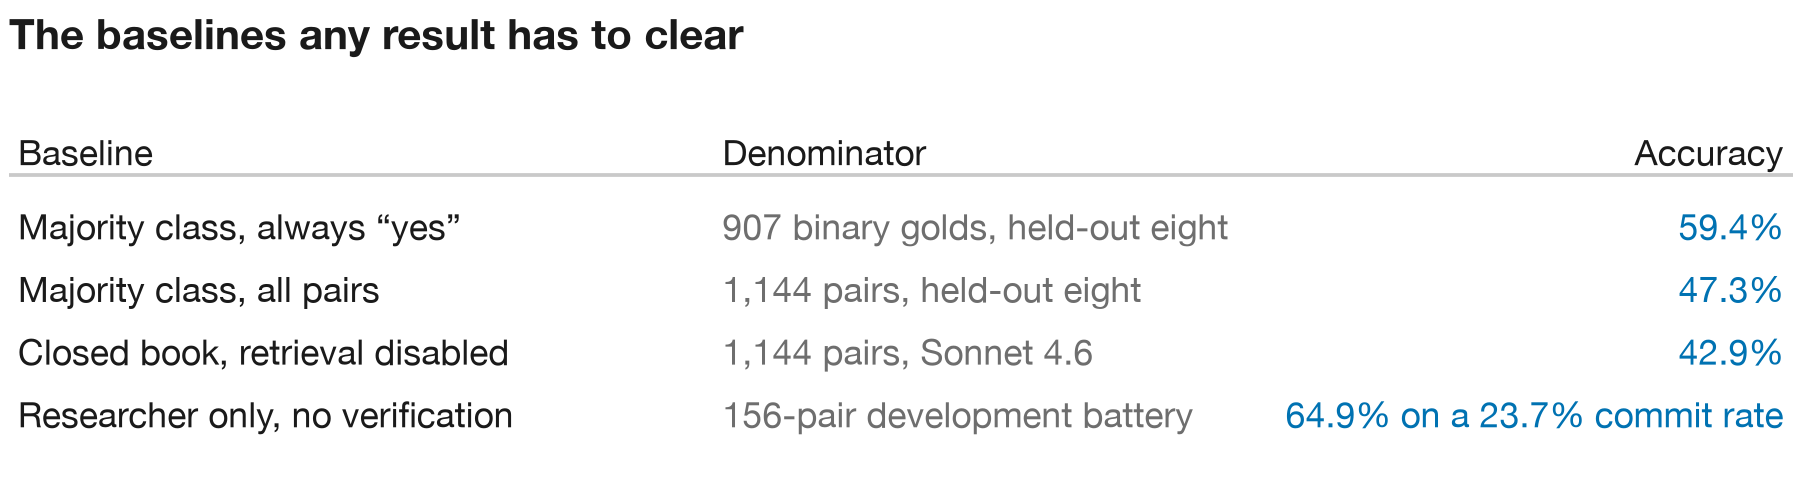
\includegraphics[width=6.1in,height=1.67996in]{media/media/image23.png}

@@CL@@Table F.1: The baselines any result has to clear.@@/CL@@\textbf{@@CC@@ @@/CC@@}

{\def\LTcaptype{none} % do not increment counter
\begin{longtable}[]{@{}
  >{\raggedright\arraybackslash}p{(\linewidth - 6\tabcolsep) * \real{0.2157}}
  >{\raggedright\arraybackslash}p{(\linewidth - 6\tabcolsep) * \real{0.3039}}
  >{\raggedright\arraybackslash}p{(\linewidth - 6\tabcolsep) * \real{0.2059}}
  >{\raggedright\arraybackslash}p{(\linewidth - 6\tabcolsep) * \real{0.2745}}@{}}
\toprule\noalign{}
\begin{minipage}[b]{\linewidth}\raggedright
\textbf{Baseline}
\end{minipage} & \begin{minipage}[b]{\linewidth}\raggedright
\textbf{What it isolates}
\end{minipage} & \begin{minipage}[b]{\linewidth}\raggedright
\textbf{Value}
\end{minipage} & \begin{minipage}[b]{\linewidth}\raggedright
\textbf{Denominator}
\end{minipage} \\
\midrule\noalign{}
\endhead
\bottomrule\noalign{}
\endlastfoot
@@CC@@Always-yes, all 36 countries@@/CC@@ & @@CC@@what no reasoning at all scores on the full assessment@@/CC@@ & @@CC@@81.8\%@@/CC@@ & @@CC@@4,146 binary golds@@/CC@@ \\
@@CC@@Always-yes, evaluation eight@@/CC@@ & @@CC@@the same, once negative golds are oversampled@@/CC@@ & @@CC@@59.4\%@@/CC@@ & @@CC@@907 binary golds@@/CC@@ \\
@@CC@@Majority class, development battery@@/CC@@ & @@CC@@the same, on the class-balanced tuning set@@/CC@@ & @@CC@@50.6\%@@/CC@@ & @@CC@@154 binary golds; the majority class here is no, not yes@@/CC@@ \\
@@CC@@Closed-book, retrieval disabled@@/CC@@ & @@CC@@how much of the answer key the model already carries@@/CC@@ & @@CC@@42.9\%, against a 47.3\% floor@@/CC@@ & @@CC@@1,139 evaluation pairs@@/CC@@ \\
@@CC@@Researcher alone, no verification@@/CC@@ & @@CC@@what one agent reaches before any checking@@/CC@@ & @@CC@@23.7\% coverage, 64.9\% commit-accuracy@@/CC@@ & @@CC@@156-pair development battery, Sonnet 4.6@@/CC@@ \\
\end{longtable}
}

\section{@@CL@@G. The Full Question Bank@@/CL@@}\label{clg.-the-full-question-bankcl}

@@CL@@The complete ODMI questionnaire as the swarm sees it, all 143 questions in the order they appear in the instrument. This is the population every figure in Chapter 4 is drawn from, so it is here in full rather than sampled. By dimension: Policy 31, Portal 45, Quality 29 and Impact 38. By answer shape: 124 binary, 12 percentage bands, 3 ordinal magnitudes, 2 count bands and 2 categorical. The 124 binary questions are the ones the headline accuracy figures are computed over, because they are the only shape where a ``yes'' or ``no'' can be scored against the published key without a banding judgement.@@/CL@@

{\def\LTcaptype{none} % do not increment counter
\begin{longtable}[]{@{}
  >{\raggedright\arraybackslash}p{(\linewidth - 2\tabcolsep) * \real{0.1386}}
  >{\raggedright\arraybackslash}p{(\linewidth - 2\tabcolsep) * \real{0.8614}}@{}}
\toprule\noalign{}
\begin{minipage}[b]{\linewidth}\raggedright
\textbf{@@CL@@Question@@/CL@@}
\end{minipage} & \begin{minipage}[b]{\linewidth}\raggedright
\textbf{@@CL@@Text@@/CL@@}
\end{minipage} \\
\midrule\noalign{}
\endhead
\bottomrule\noalign{}
\endlastfoot
@@CL@@P1@@/CL@@ & @@CL@@Is there a national open data policy in your country and, if your country is an EU Member State, does this include a national legislation for the transposition of the Open Data Directive? For Explanation: * If yes, please provide (1) the URL and (2) title of the policy document and (3) briefly describe. * If `other', please provide (1) a brief explanation to support your answer choice and (2) provide the URL and indicate the policy section which explicitly references open data.@@/CL@@ \\
@@CL@@P2@@/CL@@ & @@CL@@Is there a national open data strategy in your country? For Explanation: * If yes, please provide (1) the URL to the strategy and (2) describe the main highlights. * If \textquotesingle not applicable\textquotesingle, please provide (1) a brief explanation to support your answer choice and provide (2) the URL and indicate the policy section which explicitly references objectives, actions/measures, delivery timelines etc.@@/CL@@ \\
@@CL@@P3@@/CL@@ & @@CL@@Is there an open data policy/strategy at regional or local level? For Explanation: * If yes, please (1) provide the URL and (2) title of the document(s) and (3) briefly describe.@@/CL@@ \\
@@CL@@P4@@/CL@@ & @@CL@@Does the national strategy/policy include an action plan with measures to be implemented in the open data field? For Explanation: If yes, please briefly describe the main measures described by the action plan.@@/CL@@ \\
@@CL@@P5@@/CL@@ & @@CL@@Does the national strategy/policy outline measures to incentivise the publication of and access to real-time or dynamic data? For Explanation: * If yes, please briefly describe the measures.@@/CL@@ \\
@@CL@@P6@@/CL@@ & @@CL@@Does the national strategy/policy outline measures to incentivise the publication of and access to citizen-generated data? For Explanation: * If yes, please briefly describe the measures.@@/CL@@ \\
@@CL@@P7@@/CL@@ & @@CL@@Does the national strategy/policy foster the discoverability of the aforementioned types of data from your country on data.europa.eu? For Explanation: * If yes, please briefly describe how.@@/CL@@ \\
@@CL@@P8@@/CL@@ & @@CL@@Does the national strategy/policy outline measures to support the reuse of open data by the public sector? For Explanation: * If yes, please briefly describe the measures.@@/CL@@ \\
@@CL@@P9@@/CL@@ & @@CL@@Does the national strategy/policy outline measures to support the reuse of open data by the private sector? For Explanation: * If yes, please briefly describe the measures.@@/CL@@ \\
@@CL@@P10-a@@/CL@@ & @@CL@@Does the national strategy/policy mandate carrying out and maintaining a data inventory by public bodies, whether at national or local level? For Explanation: * If yes, please briefly specify.@@/CL@@ \\
@@CL@@P10-b@@/CL@@ & @@CL@@Do these data inventories include the data collected by public bodies that cannot be published as open data (e.g. in relation to the EU Data Governance Act (EU) 2022/868)? For Explanation: * If yes, please briefly specify.@@/CL@@ \\
@@CL@@P11@@/CL@@ & @@CL@@Is your country applying the implementing regulation (EU) 2023/138 on high-value datasets? For Explanation: * If yes, how is it progressing? * If you are an EFTA or a candidate country to the EU, please select \textquotesingle not applicable\textquotesingle. ** In the table below, please indicate your progress with respect to a) organisation, b) legal aspects, c) technical aspects on a scale from 1 to 5. 1 = no progress; 2 = few progress; 3 = some progress; 4 = considerable progress; 5 = works are finalised.@@/CL@@ \\
@@CL@@P12@@/CL@@ & @@CL@@Have the public bodies in your country denoted relevant datasets as high-value datasets in their metadata following the publication of the implementing regulation (EU) 2023/138 on high-value datasets? For Explanation: * If yes, please specify how and highlight challenges, if any. * If you are an EFTA or a candidate country to the EU, please select \textquotesingle not applicable\textquotesingle.@@/CL@@ \\
@@CL@@P13@@/CL@@ & @@CL@@Is there a governance structure in place that enables the participation and/or inclusion of various open data stakeholders? For Explanation: * If yes, please briefly describe the governance structure and its operating model@@/CL@@ \\
@@CL@@P14@@/CL@@ & @@CL@@How would you classify the model used for governing open data in your country? For Explanation: * Please briefly explain why this model was chosen/works best for your country@@/CL@@ \\
@@CL@@P15@@/CL@@ & @@CL@@Does the governance structure ensure that the local and regional open data initiatives are facilitated and supported at national level? For Explanation: * If yes, please give an example of what kind of support. * If not applicable, please explain why.@@/CL@@ \\
@@CL@@P16@@/CL@@ & @@CL@@To what degree do local/regional public bodies conduct open data initiatives? For Explanation: * If not applicable, please explain why.@@/CL@@ \\
@@CL@@P17@@/CL@@ & @@CL@@Is a document describing the responsibilities and governance structure of the national (and/or regional/local) open data team publicly available? For Explanation: * If yes, please provide the URL where this information is published.@@/CL@@ \\
@@CL@@P18@@/CL@@ & @@CL@@Is there a regular exchange of knowledge or experiences between the national open data team and the team maintaining the national portal? For Explanation: * If yes, please briefly describe how this exchange takes place and provide evidence supporting your answer (e.g. meeting agendas, URLs to news items).@@/CL@@ \\
@@CL@@P19@@/CL@@ & @@CL@@Does the governance model include the appointment of official roles in civil services that are dedicated to open data (e.g. open data officers)? For Explanation: * If yes, please describe how this task is fulfilled at public body level.@@/CL@@ \\
@@CL@@P20@@/CL@@ & @@CL@@Is there a regular exchange of knowledge or experiences between the national open data team and the wider network of open data officers in your country? For Explanation: * If yes, please briefly describe how this exchange takes place and provide evidence supporting your answer (e.g. meeting agendas, URLs to news items).@@/CL@@ \\
@@CL@@P21@@/CL@@ & @@CL@@Is there a regular exchange of knowledge or experiences between public sector bodies (i.e. the providers) and open data reusers (e.g. academia, citizens, businesses)? For Explanation: * If yes, please briefly describe how this exchange takes place and provide evidence supporting your answer (e.g. meeting agendas, URLs to news items).@@/CL@@ \\
@@CL@@P22@@/CL@@ & @@CL@@Do data publication plans exist at public body level? For Explanation: * If yes, please provide the URL and briefly highlight the key aspects covered.@@/CL@@ \\
@@CL@@P23@@/CL@@ & @@CL@@Are there processes to ensure that the open data policies/strategy previously mentioned are implemented (e.g. monitoring)? For Explanation: * If yes, please specify the process(es).@@/CL@@ \\
@@CL@@P24@@/CL@@ & @@CL@@Are there processes to ensure that the open data policies/strategy previously mentioned are updated and revised as needed? For explanation: * If yes, please describe the process and any recent updates made to strategy/policy@@/CL@@ \\
@@CL@@P25@@/CL@@ & @@CL@@Are there any processes in place to assess if public sector bodies are charging for data above marginal cost? (please see directive (EU) 2019/1024 on open data and the reuse of public sector information). For Explanation: * If yes, please specify the process(es).@@/CL@@ \\
@@CL@@P26-a@@/CL@@ & @@CL@@What are the top 3 challenges that your country is facing in the implementation of the mentioned open data policies/strategy? For Explanation: * Please briefly describe.@@/CL@@ \\
@@CL@@P26-b@@/CL@@ & @@CL@@Are there activities in place to address these challenges in your country (e.g. with specific national/regional/local plans or initiatives)? For Explanation: * If yes, please briefly describe the measures that you have adopted or plan to adopt to address these challenges. * If no, please specify what is hampering finding a strategic approach to solve these challenges.@@/CL@@ \\
@@CL@@P27@@/CL@@ & @@CL@@Are there any activities in place to assist data holders with publishing their data as open data (i.e. to help them with the data opening process)? For Explanation: * If yes, please describe/provide examples of these activities.@@/CL@@ \\
@@CL@@P28@@/CL@@ & @@CL@@Is there a professional development or training plan for civil servants working with data in your country? For Explanation: * If yes, please briefly describe these training activities.@@/CL@@ \\
@@CL@@P29@@/CL@@ & @@CL@@Are there annually held national, regional or local events (e.g. hackathons, courses, conferences, users meet-ups, summer/winter schools) to promote open data and open data literacy in your country beyond the target group of public servants? For Explanation: * If yes, please provide examples (e.g. title, date, location of the event and URL).@@/CL@@ \\
@@CL@@PT1@@/CL@@ & @@CL@@Is there a national portal in your country for that enables users to search for open datasets and find where to download open data? For Explanation: * If yes, please provide the URL of the national portal.@@/CL@@ \\
@@CL@@PT2@@/CL@@ & @@CL@@For Explanation: * What is the technology stack of your portal (e.g. based on uData, CKAN, etc.)@@/CL@@ \\
@@CL@@PT3@@/CL@@ & @@CL@@Does the national portal offer to its users a way to programmatically query the metadata via an API? For Explanation: * If yes, please provide the direct-URL to this feature.@@/CL@@ \\
@@CL@@PT4@@/CL@@ & @@CL@@Does the national portal offer to its users a way to programmatically query the metadata via a SPARQL access point? For Explanation: * If yes, please provide the direct-URL to this feature.@@/CL@@ \\
@@CL@@PT5@@/CL@@ & @@CL@@Does the national portal offer/link to documentation on the use of APIs? For Explanation: * If yes, please provide the direct-URL to this feature.@@/CL@@ \\
@@CL@@PT6@@/CL@@ & @@CL@@Does the national portal offer/link to documentation on the use of SPARQL? For Explanation: * If yes, please provide the direct-URL to this feature.@@/CL@@ \\
@@CL@@PT7@@/CL@@ & @@CL@@Does the national portal provide functionality for users to contribute datasets they have produced or enriched? For explanation: * If yes, please (1) explain how the portal facilitate the linking of documentation and supporting materials to these user-contributed datasets and (2) provide the direct-URL to this feature.@@/CL@@ \\
@@CL@@PT8@@/CL@@ & @@CL@@Does the national portal offer a mechanism for users to provide general feedback, such a \textquotesingle Contact us\textquotesingle{} or \textquotesingle Feedback\textquotesingle{} button that is placed in a visible spot and would allows users to send a general comment concerning the portal? For Explanation: * If yes, please provide the direct-URL to this feature or describe how this functionality is provided.@@/CL@@ \\
@@CL@@PT9@@/CL@@ & @@CL@@Does the national portal offer a mechanism for users to provide feedback on specific datasets, such as a \textquotesingle feedback button\textquotesingle{} or a comment/discussion section under the dataset? For Explanation: * If yes, please provide the direct-URL to this feature or describe how this functionality is provided.@@/CL@@ \\
@@CL@@PT10@@/CL@@ & @@CL@@Does the national portal provide a mechanism for users to rate datasets? For Explanation: * If yes, please provide the direct-URL to this feature or describe how this functionality is provided.@@/CL@@ \\
@@CL@@PT11@@/CL@@ & @@CL@@Does the national portal enable users to find information and news on relevant open data topics in the country? For Explanation: * If yes, please provide the direct-URL to this feature.@@/CL@@ \\
@@CL@@PT12@@/CL@@ & @@CL@@Does the national portal offer the possibility for users to receive notifications when new datasets are available on the national portal (RSS, ATOM feeds, email notifications etc.)? For Explanation: * If yes, please provide the direct-URL to this feature.@@/CL@@ \\
@@CL@@PT13@@/CL@@ & @@CL@@Does the national portal enable users to request datasets, such as through a "request data" button? For Explanation: * If yes, please provide the direct-URL to this feature or describe how this functionality is provided.@@/CL@@ \\
@@CL@@PT14@@/CL@@ & @@CL@@Are requests for datasets and their progress status presented in a transparent manner on the national portal? For Explanation: * If yes, please provide the direct-URL to this feature.@@/CL@@ \\
@@CL@@PT15@@/CL@@ & @@CL@@Does the team monitor the extent to which requests (either via the portal or otherwise) result in the publication of the requested data? For Explanation: * If yes, please describe how this monitoring is conducted.@@/CL@@ \\
@@CL@@PT16@@/CL@@ & @@CL@@Does the national portal offer a mechanism for users to exchange with others, such as a discussion forum? For Explanation: * If yes, please provide the direct-URL to this feature or describe how this functionality is provided.@@/CL@@ \\
@@CL@@PT17@@/CL@@ & @@CL@@Does the national portal showcase reuse cases, such as in a designated section of the portal? For Explanation: * If yes, please provide the direct-URL to this feature.@@/CL@@ \\
@@CL@@PT18@@/CL@@ & @@CL@@Does the national portal reference the datasets that the showcased reuse cases are based on (i.e. there is a link between the reuse case in the showcase and the underlying dataset on the portal)? For Explanation: * If yes, please provide the URL to this feature/to an example documenting this feature.@@/CL@@ \\
@@CL@@PT19@@/CL@@ & @@CL@@Does the national portal provide the possibility for users to submit their own reuse cases? For Explanation: * If yes, please provide the direct-URL to this feature.@@/CL@@ \\
@@CL@@PT20@@/CL@@ & @@CL@@Does the national portal offer a preview function for tabular data? For Explanation: * If yes, please provide the URL to an example documenting this feature.@@/CL@@ \\
@@CL@@PT21@@/CL@@ & @@CL@@Does the national portal offer a preview function for geospatial data? For Explanation: * If yes, please provide the URL to an example documenting this feature.@@/CL@@ \\
@@CL@@PT22@@/CL@@ & @@CL@@Do you promote high-value datasets on your national portal (e.g. use filtering features for reusers to easily find such datasets, use editorial features to promote the datasets, etc.))? For Explanation: * If yes, please specify how and highlight challenges if any. * If you are an EFTA or a candidate country to the EU, please select \textquotesingle not applicable\textquotesingle.@@/CL@@ \\
@@CL@@PT23@@/CL@@ & @@CL@@Do you monitor the portal\textquotesingle s traffic (e.g. in terms of number of unique visitors, visitor profiles, percentage of machine traffic, number of downloads according to the number of datasets etc.)? For Explanation: * If yes, which tool(s) do you use?@@/CL@@ \\
@@CL@@PT24@@/CL@@ & @@CL@@Do you run analytics on API usage? For Explanation: * If yes, please briefly (1) describe your process and (2) how you use the insights to improve the portal@@/CL@@ \\
@@CL@@PT25@@/CL@@ & @@CL@@Besides monitoring portal traffic, do you perform any further activities to better understand the behaviour and needs of users of your portal (e.g. web analytics, surveys, or analysis of social media feeds)? For Explanation: * If yes, please (1) specify the activities and explain (2) how they help you understand user needs@@/CL@@ \\
@@CL@@PT26@@/CL@@ & @@CL@@Do you use the insights about portal usage and about the behaviour and needs of portal users to improve the portal accordingly? For Explanation: * If yes, please explain your process for improving the portal based on user insights and feedback * If relevant, kindly highlight some improvements made in the past year@@/CL@@ \\
@@CL@@PT27@@/CL@@ & @@CL@@Do you undertake any activities to promote the portal and attract new users or new audiences? For explanation: * If yes, please (1) explain what activities your perform, and (2) mention if these activities are directed at any specific target audience (e.g. business, public sector, academia, etc.)@@/CL@@ \\
@@CL@@PT28@@/CL@@ & @@CL@@Do you monitor what keywords are used to search for data and content on the portal? For Explanation: * If yes, please briefly (1) describe your process and (2) how you use the insights to improve the portal@@/CL@@ \\
@@CL@@PT29@@/CL@@ & @@CL@@Do you monitor the most and least consulted pages? For Explanation: * If yes, please briefly (1) describe your process and (2) how you use the insights to improve the portal * For informational purposes, kindly provide the URLs to the five most popular datasets on the portal@@/CL@@ \\
@@CL@@PT30@@/CL@@ & @@CL@@Do you take measures to optimise the search and discoverability of content (data and editorial)? For Explanation: *If yes, please briefly describe how your optimise the search@@/CL@@ \\
@@CL@@PT31@@/CL@@ & @@CL@@Is the metadata on your portal available in clear plain language to enable both humans and machines to read and understand it? For Explanation: *If yes, please provide the URL to an example documenting this feature.@@/CL@@ \\
@@CL@@PT32@@/CL@@ & @@CL@@To what degree do public sector data providers contribute data to the portal? For Explanation: *Please describe what is the agreed approach. * If less than the majority of data providers, please briefly explain why (e.g. technical incompatibilities, governance aspects, low awareness etc.).@@/CL@@ \\
@@CL@@PT33@@/CL@@ & @@CL@@Do you identify the data providers that are not yet publishing data on the national portal?@@/CL@@ \\
@@CL@@PT34@@/CL@@ & @@CL@@Were there concrete actions taken to assist these data providers with their publication process? For Explanation: * If yes, could you provide some examples of the actions taken in this regard.@@/CL@@ \\
@@CL@@PT35@@/CL@@ & @@CL@@Besides the national open data portal, are there other regional and local portals? For Explanation: * If yes, please provide a complete list and the links to these portals.@@/CL@@ \\
@@CL@@PT36@@/CL@@ & @@CL@@Are regional and local portals listed above and their data sources discoverable via the national portal? For Explanation: * If not applicable, please briefly explain why.@@/CL@@ \\
@@CL@@PT37@@/CL@@ & @@CL@@To what degree are regional and local sources harvested automatically? For Explanation: * If less than the majority of existing sources is harvested by the national portal, please briefly explain why. * If not applicable, please briefly explain why.@@/CL@@ \\
@@CL@@PT38@@/CL@@ & @@CL@@Does the national portal include datasets that are real-time or dynamic? For Explanation: * If yes, please provide URLs to real-time and/or dynamic data featured via the national portal.@@/CL@@ \\
@@CL@@PT39@@/CL@@ & @@CL@@Does the national portal provide a way for non-official data (i.e. not stemming from official sources, such as community-sourced/citizen-generated data) to be published? For Explanation: * If yes, please explain how non-official data is distinguished for official data (e.g. using a different section of the portal or tags) * And please provide a URL to an example of a non-official dataset on the portal@@/CL@@ \\
@@CL@@PT40@@/CL@@ & @@CL@@Does the national portal allow users to see what data exists but cannot be made available as open data? For Explanation: * If yes, please (1) provide the URL to an example and (2) briefly describe the approach used to ensure this transparency.@@/CL@@ \\
@@CL@@PT41@@/CL@@ & @@CL@@Does the national portal have a strategy to ensure its sustainability? For Explanation: * If yes, please (1) provide the URL to this document and (2) describe the main measures to keep the portal running in the long-term and continue to serve its audience@@/CL@@ \\
@@CL@@PT42@@/CL@@ & @@CL@@Is your national portal active on social media? For Explanation: * If yes, please provide the URL(s) to your social media accounts.@@/CL@@ \\
@@CL@@PT43@@/CL@@ & @@CL@@Are the portal's source code and relevant documentation and artefacts made available to the public (e.g. on platforms such as GitHub or GitLab)? For Explanation: *If yes, please provide the (1) platform name and (2) the URL to the portal's account on this platform.@@/CL@@ \\
@@CL@@PT44@@/CL@@ & @@CL@@Do you monitor the characteristics of the data published on the portal, such as the distribution across categories, static vs. real-time data and how these change over time? For Explanation: * If yes, please provide the direct-URL to this feature@@/CL@@ \\
@@CL@@PT45@@/CL@@ & @@CL@@Does this monitoring enable the portal team and/or data providers to take action to improve their performance on the national portal? For Explanation: * If yes, please (1) explain how and (2) if applicable provide the direct-URL to this feature.@@/CL@@ \\
@@CL@@Q1@@/CL@@ & @@CL@@Is there a pre-defined approach to ensure that metadata is kept up-to-date? For Explanation: * If yes, please briefly describe your approach.@@/CL@@ \\
@@CL@@Q2@@/CL@@ & @@CL@@What percentage of the metadata on the national portal is obtained from the source automatically, rather than edited manually? For Explanation: * Please describe (1) the workflows you have to automate the harvesting of metadata and (2) for which types of data these apply to@@/CL@@ \\
@@CL@@Q3@@/CL@@ & @@CL@@What is the average delay from the moment the metadata describing a dataset is updated at the source, and the moment the change is visible on the portal? For Explanation: * Please explain the approach for updating metadata in a timely manner@@/CL@@ \\
@@CL@@Q4@@/CL@@ & @@CL@@Do you undertake efforts to ensure that published data covers the full period from when it was first published until today, for example, the complete time series? For Explanation: * If yes, please explain the measures in place to ensure complete series of datasets@@/CL@@ \\
@@CL@@Q5@@/CL@@ & @@CL@@Have you implemented the DCAT-AP High Value Datasets tag to denote the High-Value Datasets in your (national) open data portal(s)? For Explanation: * If yes, please specify how and highlight challenges if any. * If you are an EFTA or a candidate country to the EU, please select \textquotesingle not applicable\textquotesingle.@@/CL@@ \\
@@CL@@Q6@@/CL@@ & @@CL@@Besides the DCAT-AP tag mentioned above, have you implemented any other measures to ensure that high-value datasets ((EU) 2023/138) are interoperable with datasets of other country? For Explanation: * If yes, please specify how and highlight challenges if any. * If you are an EFTA or a candidate country to the EU, please select \textquotesingle not applicable\textquotesingle.@@/CL@@ \\
@@CL@@Q7@@/CL@@ & @@CL@@Do you monitor the quality of the metadata available on your portal? For Explanation: * If yes, please briefly explain how this monitoring takes place. * If applicable, please provide the URL to this monitoring mechanism.@@/CL@@ \\
@@CL@@Q8@@/CL@@ & @@CL@@Do you publish information on the quality of the metadata available on the portal? For Explanation: * If yes, please provide the URL to this section.@@/CL@@ \\
@@CL@@Q9@@/CL@@ & @@CL@@Do you publish guidelines (e.g. written materials) and have tools in place, to assist publishers in publishing high-quality metadata? For Explanation: * If yes, please (1) briefly describe this material and (2) provide the URLs to these materials and/or tools.@@/CL@@ \\
@@CL@@Q10@@/CL@@ & @@CL@@Do you set any standards on metadata quality that data providers must abide by (e.g. on the use of licence, minimum metadata describes, use of certain DCAT-AP properties, etc) For Explanation: * If yes, please describe the standards you have in place, i.e. what is minimum information the metadata should describe@@/CL@@ \\
@@CL@@Q11@@/CL@@ & @@CL@@Do your open data publication/licensing guidelines provide recommendations for the use of Creative Commons (CC) licences, specifically CC BY 4.0 and CC0? For Explanation: * If yes, is this mandatory (e.g. prescribed by law) or recommended? * Please provide a URL link to the guidelines@@/CL@@ \\
@@CL@@Q12@@/CL@@ & @@CL@@What percentage of the open data available on the national portal is accompanied by licensing information?@@/CL@@ \\
@@CL@@Q13@@/CL@@ & @@CL@@How many different licences are used on your portal?@@/CL@@ \\
@@CL@@Q14@@/CL@@ & @@CL@@Besides providing guidelines, are there regular activities conducted or mechanisms in place to assist publishers in supplying high-quality datasets (metadata quality and data quality)? For Explanation: * If yes, please explain the support you provide?@@/CL@@ \\
@@CL@@Q15@@/CL@@ & @@CL@@Does the national portal follow the DCAT-AP framework or, if not, are standards in place to ensure interoperability with DCAT-AP? For explanation: * If the portal follow the DCAT-AP framework, please describe how compliance with DCAT-AP is ensured * If the portal does not follow the DCAT-AP framework, please describe how interoperability with DCAT-AP is ensured@@/CL@@ \\
@@CL@@Q16@@/CL@@ & @@CL@@What is the percentage of metadata on your portal that is DCAT-AP compliant, in terms of mandatory classes?@@/CL@@ \\
@@CL@@Q17@@/CL@@ & @@CL@@What is the percentage of metadata on your portal that uses DCAT-AP recommended classes?@@/CL@@ \\
@@CL@@Q18@@/CL@@ & @@CL@@What is the percentage of metadata on your portal that uses DCAT-AP optional classes?@@/CL@@ \\
@@CL@@Q19@@/CL@@ & @@CL@@Is there a national extension of the DCAT-AP standard developed for your country? For Explanation: * If yes, please (1) briefly outline the reasons for this decision, and (2) what the main differences between the national variation and the EU standard are. * If applicable, please provide the URL to the documentation of the national DCAT-AP extension.@@/CL@@ \\
@@CL@@Q20@@/CL@@ & @@CL@@Do you investigate the most common causes for the lack of DCAT-AP compliance? For Explanation: * If yes, what are the main causes for the lack of DCAT-AP compliance?@@/CL@@ \\
@@CL@@Q21@@/CL@@ & @@CL@@What is the percentage of datasets whose metadata provides a reference to where the data can be downloaded, or its API accessed (``download-URL'' in the DCAT-AP specification)?@@/CL@@ \\
@@CL@@Q22@@/CL@@ & @@CL@@What is the percentage of datasets whose metadata provides a reference to a web page from where the data can be accessed (``access-URL in the DCAT-AP specification)?@@/CL@@ \\
@@CL@@Q23@@/CL@@ & @@CL@@Do you use a model (such as the 5-Star Open Data or FAIR) to assess the quality of deployment of data in your country? For Explanation: * If yes, please briefly describe.@@/CL@@ \\
@@CL@@Q24@@/CL@@ & @@CL@@Do you conduct activities to promote and familiarise data providers with ways to ensure higher quality data? For Explanation: * If yes, please briefly describe.@@/CL@@ \\
@@CL@@Q25@@/CL@@ & @@CL@@What percentage of datasets are made available under an open licence?@@/CL@@ \\
@@CL@@Q26@@/CL@@ & @@CL@@What percentage of licences are provided in a structured data format?@@/CL@@ \\
@@CL@@Q27@@/CL@@ & @@CL@@What percentage of datasets are provided in an open and machine-readable format?@@/CL@@ \\
@@CL@@Q28@@/CL@@ & @@CL@@What percentage of datasets consistently use Uniform Resource Identifiers?@@/CL@@ \\
@@CL@@Q29@@/CL@@ & @@CL@@What percentage of datasets link to other renowned sources to provide additional context for the users, e.g. in a linked data fashion?@@/CL@@ \\
@@CL@@I1@@/CL@@ & @@CL@@Do you have a definition of open data reuse in your country? For Explanation: * If yes, please specify it.@@/CL@@ \\
@@CL@@I2@@/CL@@ & @@CL@@Are there any processes in place to monitor the level of reuse of your country\textquotesingle s open data? For Explanation: * If yes, please (1) briefly describe these processes and (2) provide the URLs to support the answer.@@/CL@@ \\
@@CL@@I3@@/CL@@ & @@CL@@Are there any activities in place to encourage public bodies to monitor the reuse of their own published data (e.g. incentives or obligations in place for public bodies or civil servants of national government)? For Explanation: * If yes, please (1) briefly describe these activities/incentives and (2) provide the URLs to support the answer.@@/CL@@ \\
@@CL@@I4@@/CL@@ & @@CL@@Does your country have processes in place to monitor and measure the level of reuse of high-value datasets ((EU) 2023/138)? For Explanation: * If yes, please specify how and highlight challenges if any. * If you are an EFTA or a candidate country to the EU, please select \textquotesingle not applicable\textquotesingle.@@/CL@@ \\
@@CL@@I5@@/CL@@ & @@CL@@Has your government specified what \textquotesingle impact of open data\textquotesingle{} means (e.g. in a strategy document)? For Explanation: * If yes, how do you define the impact of open data in your country? * If possible, please provide a URL to a public document describing it.@@/CL@@ \\
@@CL@@I6@@/CL@@ & @@CL@@Do you have a methodology in place to measure the impact of open data in your country? For Explanation: * If yes, please briefly describe the key points of this methodology.@@/CL@@ \\
@@CL@@I7@@/CL@@ & @@CL@@Is there collaboration between government and civil society or academia to create open data impact in your country? For Explanation: * If yes, please provide an example * If possible, URLs to such projects and collaborations.@@/CL@@ \\
@@CL@@I8@@/CL@@ & @@CL@@Have any public bodies in your country launched or performed any activities in the past year to understand which and how (open) datasets are reused? For Explanation: * If yes, which of the following activities? * Multiple answers are possible.@@/CL@@ \\
@@CL@@I8-a@@/CL@@ & @@CL@@Automated feedback mechanisms tracking users´ access to datasets@@/CL@@ \\
@@CL@@I8-b@@/CL@@ & @@CL@@Surveys@@/CL@@ \\
@@CL@@I8-c@@/CL@@ & @@CL@@Interviews/workshops with reusers@@/CL@@ \\
@@CL@@I8-d@@/CL@@ & @@CL@@Other@@/CL@@ \\
@@CL@@I9@@/CL@@ & @@CL@@Have any public bodies in your country launched or performed any activities in the past year to better understand reusers\textquotesingle{} needs in order to further stimulate the reuse of open data? For Explanation: * If yes, which of the following activities have been performed? Please describe how the activity has helped you better stimulate reuse. * Multiple answers are possible.@@/CL@@ \\
@@CL@@I9-a@@/CL@@ & @@CL@@Regular feedback sessions with portal users@@/CL@@ \\
@@CL@@I9-b@@/CL@@ & @@CL@@Social media sentiment analysis@@/CL@@ \\
@@CL@@I9-c@@/CL@@ & @@CL@@Other@@/CL@@ \\
@@CL@@I10@@/CL@@ & @@CL@@Have any public bodies in your country developed any systematic way of gathering reuse cases? For Explanation: * If yes, please provide a brief explanation of the process: How does the gathering happen?@@/CL@@ \\
@@CL@@I11@@/CL@@ & @@CL@@Are there any public bodies in your country that have developed a systematic ways of classifying the gathered reuse cases? For Explanation: * If yes, please provide a brief explanation of the process: According to which categories are reuse cases classified (e.g. by policy field)?@@/CL@@ \\
@@CL@@I12@@/CL@@ & @@CL@@Is any data on the impact created by open data on governmental challenges (e.g. efficiency, effectiveness, transparency, decision-making capacity) available in your country such as from research studies, impact assessments, or other systematic investigations that quantify the results or broader effects of open data being reused? For Explanation: * If yes, please (1) specify what kind of data source proves this impact and (2) provide the URLs to this data.@@/CL@@ \\
@@CL@@I13@@/CL@@ & @@CL@@Is the use of open data in your country having an impact on the efficiency and effectiveness of the government (at any level) in delivering public services? For Explanation: * If yes, please provide an example of one reuse case. For this reuse case, please provide (1) a URL to the reuse case, (2) a URL to the open dataset used by the reuse case, and (3) a description of the reuse case and its impact in this sub-domain.@@/CL@@ \\
@@CL@@I14@@/CL@@ & @@CL@@Is the use of open data in your country having an impact on transparency and accountability of public administrations? For Explanation: * If yes, please provide an example of one reuse case. For this reuse case, please provide (1) a URL to the reuse case, (2) a URL to the open dataset used by the reuse case, and (3) a description of the reuse case and its impact in this sub-domain.@@/CL@@ \\
@@CL@@I15@@/CL@@ & @@CL@@Is the use of open data in your country having an impact on policy-making processes (i.e. are public administrations making use of the data as evidence for the problem identification and policy formulation)? For Explanation: * If yes, please provide an example of one reuse case. For this reuse case, please provide (1) a URL to the reuse case, (2) a URL to the open dataset used by the reuse case, and (3) a description of the reuse case and its impact in this sub-domain.@@/CL@@ \\
@@CL@@I16@@/CL@@ & @@CL@@Is the use of open data in your country having an impact on decision-making processes (i.e. are public administrations making use of the data as evidence to be included in their daily operations)? For Explanation: * If yes, please provide an example of one reuse case. For this reuse case, please provide (1) a URL to the reuse case, (2) a URL to the open dataset used by the reuse case, and (3) a description of the reuse case and its impact in this sub-domain.@@/CL@@ \\
@@CL@@I17@@/CL@@ & @@CL@@Is any data on the impact created by open data on social challenges (e.g. inequality, healthcare, education) available in your country such as from research studies, impact assessments, or other systematic investigations that quantify the results or broader effects of open data being reused? For Explanation: * If yes, please (1) specify what kind of data source proves this impact and (2) provide the URLs to this data.@@/CL@@ \\
@@CL@@I18@@/CL@@ & @@CL@@Is the use of open data in your country having an impact on society´s ability to reduce inequality and better include minorities, migrants, and/or refugees? For Explanation: * If yes, please provide an example of one reuse case. For this reuse case, please provide (1) a URL to the reuse case, (2) a URL to the open dataset used by the reuse case, and (3) a description of the reuse case and its impact in this sub-domain.@@/CL@@ \\
@@CL@@I19@@/CL@@ & @@CL@@Is the use of open data in your country having an impact on issues about housing in urban areas? For Explanation: * If yes, please provide an example of one reuse case. For this reuse case, please provide (1) a URL to the reuse case, (2) a URL to the open dataset used by the reuse case, and (3) a description of the reuse case and its impact in this sub-domain.@@/CL@@ \\
@@CL@@I20@@/CL@@ & @@CL@@Is the use of open data in your country having an impact on the issues of health and wellbeing? For Explanation: * If yes, please provide an example of one reuse case. For this reuse case, please provide (1) a URL to the reuse case, (2) a URL to the open dataset used by the reuse case, and (3) a description of the reuse case and its impact in this sub-domain.@@/CL@@ \\
@@CL@@I21@@/CL@@ & @@CL@@Is the use of open data in your country having an impact on the society´s level of education and skills (e.g. data literacy)? For Explanation: * If yes, please provide an example of one reuse case. For this reuse case, please provide (1) a URL to the reuse case, (2) a URL to the open dataset used by the reuse case, and (3) a description of the reuse case and its impact in this sub-domain.@@/CL@@ \\
@@CL@@I22@@/CL@@ & @@CL@@Is any data on the impact created by open data on environmental challenges (e.g. climate change and environmental degradation, as highlighted in the European Green Deal) available in your country such as from research studies, impact assessments, or other systematic investigations that quantify the results or broader effects of open data being reused? For Explanation: * If yes, please specify (1) what kind of data source proves this impact and (2) provide the URLs to this data.@@/CL@@ \\
@@CL@@I23@@/CL@@ & @@CL@@Is the use of open data in your country having an impact on the level of protection of biodiversity (e.g. maintaining a good air and water quality)? For Explanation: * If yes, please provide an example of one reuse case. For this reuse case, please provide (1) a URL to the reuse case, (2) a URL to the open dataset used by the reuse case, and (3) a description of the reuse case and its impact in this sub-domain.@@/CL@@ \\
@@CL@@I24@@/CL@@ & @@CL@@Is the use of open data in your country having an impact on the achievement of more environment-friendly cities (e.g., environment-friendly transport systems, waste management etc.)? For Explanation: * If yes, please provide an example of one reuse case. For this reuse case, please provide (1) a URL to the reuse case, (2) a URL to the open dataset used by the reuse case, and (3) a description of the reuse case and its impact in this sub-domain.@@/CL@@ \\
@@CL@@I25@@/CL@@ & @@CL@@Is the use of open data in your country having an impact on the fight against climate change, for example by undertaking predictive monitoring, preventive actions, or a differentiated response to connected disasters? For Explanation: * If yes, please provide an example of one reuse case. For this reuse case, please provide (1) a URL to the reuse case, (2) a URL to the open dataset used by the reuse case, and (3) a description of the reuse case and its impact in this sub-domain.@@/CL@@ \\
@@CL@@I26@@/CL@@ & @@CL@@Is the use of open data in your country having an impact on the consumption of energy based on fuel and the switch to renewables? For Explanation: * If yes, please provide an example of one reuse case. For this reuse case, please provide (1) a URL to the reuse case, (2) a URL to the open dataset used by the reuse case, and (3) a description of the reuse case and its impact in this sub-domain.@@/CL@@ \\
@@CL@@I27@@/CL@@ & @@CL@@Is any data on the economic impact (e.g. GDP, employment, productivity, innovation, new businesses created etc.) of open data available in your country such as from research studies, impact assessments, or other systematic investigations that quantify the results or broader effects of open data being reused? For Explanation: * If yes, please specify what kind of data source proves this impact and provide the URLs to this data.@@/CL@@ \\
@@CL@@I28@@/CL@@ & @@CL@@Is the use of open data in your country having an impact on the level of employment? For Explanation: * If yes, please provide an example of one reuse case. For this reuse case, please provide (1) a URL to the reuse case, (2) a URL to the open dataset used by the reuse case, and (3) a description of the reuse case and its impact in this sub-domain.@@/CL@@ \\
@@CL@@I29@@/CL@@ & @@CL@@Is the use of open data in your country having an impact on the level of innovation and the adoption of new technologies? For Explanation: * If yes, please provide an example of one reuse case. For this reuse case, please provide (1) a URL to the reuse case, (2) a URL to the open dataset used by the reuse case, and (3) a description of the reuse case and its impact in this sub-domain.@@/CL@@ \\
@@CL@@I30@@/CL@@ & @@CL@@Is the use of open data in your country having an impact on the level of entrepreneurship (especially of women and minorities) and business creation (especially with Small- and Medium-sized Enterprises)? For Explanation: * If yes, please provide an example of one reuse case. For this reuse case, please provide (1) a URL to the reuse case, (2) a URL to the open dataset used by the reuse case, and (3) a description of the reuse case and its impact in this sub-domain.@@/CL@@ \\
@@CL@@I31@@/CL@@ & @@CL@@Is the use of open data in your country having an impact on the level of productivity? For Explanation: * If yes, please provide an example of one reuse case. For this reuse case, please provide (1) a URL to the reuse case, (2) a URL to the open dataset used by the reuse case, and (3) a description of the reuse case and its impact in this sub-domain.@@/CL@@ \\
\end{longtable}
}

@@CL@@Table G.1: All 143 questions of the 2025 ODMI questionnaire.@@/CL@@

\section{@@CL@@H. The Catalogue Recompute in Full@@/CL@@}\label{clh.-the-catalogue-recompute-in-fullcl}

@@CL@@The nine Quality questions the deterministic catalogue tool can answer without an agent, computed directly from a harvest of each national portal. §3.5 reports the agreement rate; the underlying numbers are here. Two things to read carefully. The harvest is a snapshot, so a country\textquotesingle s figure is only as current as the fetch date in the first table, and France\textquotesingle s harvest is marked partial, meaning the portal was paged rather than exhausted. Estonia returned nothing at all and is kept in the table as a record of the attempt. Where the computed band and the published answer disagree the disagreement is real and unresolved, not an error corrected here.@@/CL@@

\textbf{@@CL@@What was harvested@@/CL@@}

{\def\LTcaptype{none} % do not increment counter
\begin{longtable}[]{@{}
  >{\raggedright\arraybackslash}p{(\linewidth - 8\tabcolsep) * \real{0.1181}}
  >{\raggedright\arraybackslash}p{(\linewidth - 8\tabcolsep) * \real{0.1869}}
  >{\raggedright\arraybackslash}p{(\linewidth - 8\tabcolsep) * \real{0.1476}}
  >{\raggedright\arraybackslash}p{(\linewidth - 8\tabcolsep) * \real{0.1574}}
  >{\raggedright\arraybackslash}p{(\linewidth - 8\tabcolsep) * \real{0.1574}}@{}}
\toprule\noalign{}
\begin{minipage}[b]{\linewidth}\raggedright
\textbf{@@CL@@Country@@/CL@@}
\end{minipage} & \begin{minipage}[b]{\linewidth}\raggedright
\textbf{@@CL@@Route@@/CL@@}
\end{minipage} & \begin{minipage}[b]{\linewidth}\raggedright
\textbf{@@CL@@Datasets@@/CL@@}
\end{minipage} & \begin{minipage}[b]{\linewidth}\raggedright
\textbf{@@CL@@Fetched@@/CL@@}
\end{minipage} & \begin{minipage}[b]{\linewidth}\raggedright
\textbf{@@CL@@Harvest@@/CL@@}
\end{minipage} \\
\midrule\noalign{}
\endhead
\bottomrule\noalign{}
\endlastfoot
@@CL@@AL@@/CL@@ & @@CL@@al\_dcat\_api@@/CL@@ & @@CL@@130@@/CL@@ & @@CL@@2026-06-25@@/CL@@ & @@CL@@complete@@/CL@@ \\
@@CL@@DE@@/CL@@ & @@CL@@dcat\_rdf@@/CL@@ & @@CL@@3,000@@/CL@@ & @@CL@@2026-06-02@@/CL@@ & @@CL@@complete@@/CL@@ \\
@@CL@@EE@@/CL@@ & @@CL@@estonia\_json@@/CL@@ & @@CL@@0@@/CL@@ & @@CL@@2026-06-02@@/CL@@ & @@CL@@partial@@/CL@@ \\
@@CL@@FI@@/CL@@ & @@CL@@ckan\_json@@/CL@@ & @@CL@@2,525@@/CL@@ & @@CL@@2026-06-24@@/CL@@ & @@CL@@complete@@/CL@@ \\
@@CL@@FR@@/CL@@ & @@CL@@dcat\_rdf@@/CL@@ & @@CL@@3,400@@/CL@@ & @@CL@@2026-07-17@@/CL@@ & @@CL@@partial@@/CL@@ \\
@@CL@@HR@@/CL@@ & @@CL@@sparql\_rdf@@/CL@@ & @@CL@@3,867@@/CL@@ & @@CL@@2026-07-17@@/CL@@ & @@CL@@complete@@/CL@@ \\
@@CL@@HU@@/CL@@ & @@CL@@ckan\_json@@/CL@@ & @@CL@@2,282@@/CL@@ & @@CL@@2026-06-02@@/CL@@ & @@CL@@complete@@/CL@@ \\
@@CL@@NL@@/CL@@ & @@CL@@ckan\_json@@/CL@@ & @@CL@@20,772@@/CL@@ & @@CL@@2026-06-02@@/CL@@ & @@CL@@complete@@/CL@@ \\
@@CL@@RO@@/CL@@ & @@CL@@ckan\_json@@/CL@@ & @@CL@@5,143@@/CL@@ & @@CL@@2026-06-02@@/CL@@ & @@CL@@complete@@/CL@@ \\
@@CL@@SE@@/CL@@ & @@CL@@sparql\_rdf@@/CL@@ & @@CL@@23,305@@/CL@@ & @@CL@@2026-07-17@@/CL@@ & @@CL@@complete@@/CL@@ \\
\end{longtable}
}

@@CL@@Table H.1: The portal harvest behind every catalogue figure.@@/CL@@

\textbf{@@CL@@What the harvest computes, against the published answer@@/CL@@}

{\def\LTcaptype{none} % do not increment counter
\begin{longtable}[]{@{}
  >{\raggedright\arraybackslash}p{(\linewidth - 8\tabcolsep) * \real{0.1274}}
  >{\raggedright\arraybackslash}p{(\linewidth - 8\tabcolsep) * \real{0.1177}}
  >{\raggedright\arraybackslash}p{(\linewidth - 8\tabcolsep) * \real{0.3333}}
  >{\raggedright\arraybackslash}p{(\linewidth - 8\tabcolsep) * \real{0.1470}}
  >{\raggedright\arraybackslash}p{(\linewidth - 8\tabcolsep) * \real{0.2745}}@{}}
\toprule\noalign{}
\begin{minipage}[b]{\linewidth}\raggedright
\textbf{@@CL@@Question@@/CL@@}
\end{minipage} & \begin{minipage}[b]{\linewidth}\raggedright
\textbf{@@CL@@Country@@/CL@@}
\end{minipage} & \begin{minipage}[b]{\linewidth}\raggedright
\textbf{@@CL@@Computed@@/CL@@}
\end{minipage} & \begin{minipage}[b]{\linewidth}\raggedright
\textbf{@@CL@@Band@@/CL@@}
\end{minipage} & \begin{minipage}[b]{\linewidth}\raggedright
\textbf{@@CL@@Published@@/CL@@}
\end{minipage} \\
\midrule\noalign{}
\endhead
\bottomrule\noalign{}
\endlastfoot
@@CL@@Q12@@/CL@@ & @@CL@@AL@@/CL@@ & @@CL@@100.0\% (130/130)@@/CL@@ & @@CL@@\textgreater90\%@@/CL@@ & @@CL@@\textgreater90\%@@/CL@@ \\
@@CL@@Q12@@/CL@@ & @@CL@@DE@@/CL@@ & @@CL@@100.0\% (3,000/3,000)@@/CL@@ & @@CL@@\textgreater90\%@@/CL@@ & @@CL@@\textgreater90\%@@/CL@@ \\
@@CL@@Q12@@/CL@@ & @@CL@@FI@@/CL@@ & @@CL@@96.0\% (2,424/2,525)@@/CL@@ & @@CL@@\textgreater90\%@@/CL@@ & @@CL@@\textgreater90\%@@/CL@@ \\
@@CL@@Q12@@/CL@@ & @@CL@@FR@@/CL@@ & @@CL@@24.1\% (820/3,400)@@/CL@@ & @@CL@@10-30\%@@/CL@@ & @@CL@@\textgreater90\%@@/CL@@ \\
@@CL@@Q12@@/CL@@ & @@CL@@HR@@/CL@@ & @@CL@@0.0\% (0/3,867)@@/CL@@ & @@CL@@\textless10\%@@/CL@@ & @@CL@@\textgreater90\%@@/CL@@ \\
@@CL@@Q12@@/CL@@ & @@CL@@HU@@/CL@@ & @@CL@@72.8\% (1,661/2,282)@@/CL@@ & @@CL@@71-90\%@@/CL@@ & @@CL@@\textgreater90\%@@/CL@@ \\
@@CL@@Q12@@/CL@@ & @@CL@@NL@@/CL@@ & @@CL@@96.9\% (20,131/20,772)@@/CL@@ & @@CL@@\textgreater90\%@@/CL@@ & @@CL@@\textgreater90\%@@/CL@@ \\
@@CL@@Q12@@/CL@@ & @@CL@@RO@@/CL@@ & @@CL@@96.2\% (4,946/5,143)@@/CL@@ & @@CL@@\textgreater90\%@@/CL@@ & @@CL@@\textgreater90\%@@/CL@@ \\
@@CL@@Q12@@/CL@@ & @@CL@@SE@@/CL@@ & @@CL@@63.7\% (14,834/23,305)@@/CL@@ & @@CL@@51-70\%@@/CL@@ & @@CL@@71-90\%@@/CL@@ \\
@@CL@@Q13@@/CL@@ & @@CL@@DE@@/CL@@ & @@CL@@13@@/CL@@ & @@CL@@\textgreater10@@/CL@@ & @@CL@@5-10@@/CL@@ \\
@@CL@@Q13@@/CL@@ & @@CL@@FI@@/CL@@ & @@CL@@9@@/CL@@ & @@CL@@5-10@@/CL@@ & @@CL@@5-10@@/CL@@ \\
@@CL@@Q13@@/CL@@ & @@CL@@FR@@/CL@@ & @@CL@@5@@/CL@@ & @@CL@@5-10@@/CL@@ & @@CL@@1-4@@/CL@@ \\
@@CL@@Q13@@/CL@@ & @@CL@@HR@@/CL@@ & @@CL@@0@@/CL@@ & @@CL@@\textgreater10@@/CL@@ & @@CL@@1-4@@/CL@@ \\
@@CL@@Q13@@/CL@@ & @@CL@@HU@@/CL@@ & @@CL@@2@@/CL@@ & @@CL@@1-4@@/CL@@ & @@CL@@1-4@@/CL@@ \\
@@CL@@Q13@@/CL@@ & @@CL@@NL@@/CL@@ & @@CL@@7@@/CL@@ & @@CL@@5-10@@/CL@@ & @@CL@@5-10@@/CL@@ \\
@@CL@@Q13@@/CL@@ & @@CL@@RO@@/CL@@ & @@CL@@5@@/CL@@ & @@CL@@5-10@@/CL@@ & @@CL@@1-4@@/CL@@ \\
@@CL@@Q13@@/CL@@ & @@CL@@SE@@/CL@@ & @@CL@@34@@/CL@@ & @@CL@@\textgreater10@@/CL@@ & @@CL@@\textgreater10@@/CL@@ \\
@@CL@@Q16@@/CL@@ & @@CL@@DE@@/CL@@ & @@CL@@4.2\% (42/1,000)@@/CL@@ & @@CL@@\textless10\%@@/CL@@ & @@CL@@\textgreater90\%@@/CL@@ \\
@@CL@@Q16@@/CL@@ & @@CL@@FI@@/CL@@ & @@CL@@99.3\% (993/1,000)@@/CL@@ & @@CL@@\textgreater90\%@@/CL@@ & @@CL@@\textgreater90\%@@/CL@@ \\
@@CL@@Q16@@/CL@@ & @@CL@@FR@@/CL@@ & @@CL@@80.6\% (806/1,000)@@/CL@@ & @@CL@@71-90\%@@/CL@@ & @@CL@@\textgreater90\%@@/CL@@ \\
@@CL@@Q16@@/CL@@ & @@CL@@HR@@/CL@@ & @@CL@@40.6\% (406/1,000)@@/CL@@ & @@CL@@31-50\%@@/CL@@ & @@CL@@\textgreater90\%@@/CL@@ \\
@@CL@@Q16@@/CL@@ & @@CL@@HU@@/CL@@ & @@CL@@100.0\% (1,000/1,000)@@/CL@@ & @@CL@@\textgreater90\%@@/CL@@ & @@CL@@\textgreater90\%@@/CL@@ \\
@@CL@@Q16@@/CL@@ & @@CL@@NL@@/CL@@ & @@CL@@66.6\% (666/1,000)@@/CL@@ & @@CL@@51-70\%@@/CL@@ & @@CL@@\textgreater90\%@@/CL@@ \\
@@CL@@Q16@@/CL@@ & @@CL@@RO@@/CL@@ & @@CL@@96.1\% (961/1,000)@@/CL@@ & @@CL@@\textgreater90\%@@/CL@@ & @@CL@@71-90\%@@/CL@@ \\
@@CL@@Q16@@/CL@@ & @@CL@@SE@@/CL@@ & @@CL@@98.9\% (989/1,000)@@/CL@@ & @@CL@@\textgreater90\%@@/CL@@ & @@CL@@\textgreater90\%@@/CL@@ \\
@@CL@@Q17@@/CL@@ & @@CL@@DE@@/CL@@ & @@CL@@100.0\% (3,000/3,000)@@/CL@@ & @@CL@@\textgreater90\%@@/CL@@ & @@CL@@\textgreater90\%@@/CL@@ \\
@@CL@@Q17@@/CL@@ & @@CL@@FI@@/CL@@ & @@CL@@100.0\% (2,525/2,525)@@/CL@@ & @@CL@@\textgreater90\%@@/CL@@ & @@CL@@\textgreater90\%@@/CL@@ \\
@@CL@@Q17@@/CL@@ & @@CL@@FR@@/CL@@ & @@CL@@100.0\% (3,400/3,400)@@/CL@@ & @@CL@@\textgreater90\%@@/CL@@ & @@CL@@\textgreater90\%@@/CL@@ \\
@@CL@@Q17@@/CL@@ & @@CL@@HR@@/CL@@ & @@CL@@100.0\% (3,867/3,867)@@/CL@@ & @@CL@@\textgreater90\%@@/CL@@ & @@CL@@\textgreater90\%@@/CL@@ \\
@@CL@@Q17@@/CL@@ & @@CL@@HU@@/CL@@ & @@CL@@100.0\% (2,282/2,282)@@/CL@@ & @@CL@@\textgreater90\%@@/CL@@ & @@CL@@\textgreater90\%@@/CL@@ \\
@@CL@@Q17@@/CL@@ & @@CL@@NL@@/CL@@ & @@CL@@100.0\% (20,772/20,772)@@/CL@@ & @@CL@@\textgreater90\%@@/CL@@ & @@CL@@\textgreater90\%@@/CL@@ \\
@@CL@@Q17@@/CL@@ & @@CL@@RO@@/CL@@ & @@CL@@100.0\% (5,143/5,143)@@/CL@@ & @@CL@@\textgreater90\%@@/CL@@ & @@CL@@10-30\%@@/CL@@ \\
@@CL@@Q17@@/CL@@ & @@CL@@SE@@/CL@@ & @@CL@@100.0\% (23,305/23,305)@@/CL@@ & @@CL@@\textgreater90\%@@/CL@@ & @@CL@@\textgreater90\%@@/CL@@ \\
@@CL@@Q18@@/CL@@ & @@CL@@DE@@/CL@@ & @@CL@@100.0\% (3,000/3,000)@@/CL@@ & @@CL@@\textgreater90\%@@/CL@@ & @@CL@@71-90\%@@/CL@@ \\
@@CL@@Q18@@/CL@@ & @@CL@@FI@@/CL@@ & @@CL@@98.7\% (2,492/2,525)@@/CL@@ & @@CL@@\textgreater90\%@@/CL@@ & @@CL@@\textgreater90\%@@/CL@@ \\
@@CL@@Q18@@/CL@@ & @@CL@@FR@@/CL@@ & @@CL@@100.0\% (3,400/3,400)@@/CL@@ & @@CL@@\textgreater90\%@@/CL@@ & @@CL@@\textgreater90\%@@/CL@@ \\
@@CL@@Q18@@/CL@@ & @@CL@@HR@@/CL@@ & @@CL@@100.0\% (3,867/3,867)@@/CL@@ & @@CL@@\textgreater90\%@@/CL@@ & @@CL@@\textgreater90\%@@/CL@@ \\
@@CL@@Q18@@/CL@@ & @@CL@@HU@@/CL@@ & @@CL@@100.0\% (2,282/2,282)@@/CL@@ & @@CL@@\textgreater90\%@@/CL@@ & @@CL@@\textgreater90\%@@/CL@@ \\
@@CL@@Q18@@/CL@@ & @@CL@@NL@@/CL@@ & @@CL@@86.3\% (17,925/20,772)@@/CL@@ & @@CL@@71-90\%@@/CL@@ & @@CL@@10-30\%@@/CL@@ \\
@@CL@@Q18@@/CL@@ & @@CL@@RO@@/CL@@ & @@CL@@99.7\% (5,130/5,143)@@/CL@@ & @@CL@@\textgreater90\%@@/CL@@ & @@CL@@\textless10\%@@/CL@@ \\
@@CL@@Q18@@/CL@@ & @@CL@@SE@@/CL@@ & @@CL@@94.8\% (22,098/23,305)@@/CL@@ & @@CL@@\textgreater90\%@@/CL@@ & @@CL@@51-70\%@@/CL@@ \\
@@CL@@Q21@@/CL@@ & @@CL@@AL@@/CL@@ & @@CL@@100.0\% (130/130)@@/CL@@ & @@CL@@\textgreater90\%@@/CL@@ & @@CL@@\textgreater90\%@@/CL@@ \\
@@CL@@Q21@@/CL@@ & @@CL@@DE@@/CL@@ & @@CL@@2.7\% (81/3,000)@@/CL@@ & @@CL@@\textless10\%@@/CL@@ & @@CL@@31-50\%@@/CL@@ \\
@@CL@@Q21@@/CL@@ & @@CL@@FI@@/CL@@ & @@CL@@100.0\% (2,492/2,492)@@/CL@@ & @@CL@@\textgreater90\%@@/CL@@ & @@CL@@\textgreater90\%@@/CL@@ \\
@@CL@@Q21@@/CL@@ & @@CL@@FR@@/CL@@ & @@CL@@100.0\% (1,954/1,954)@@/CL@@ & @@CL@@\textgreater90\%@@/CL@@ & @@CL@@\textgreater90\%@@/CL@@ \\
@@CL@@Q21@@/CL@@ & @@CL@@HR@@/CL@@ & @@CL@@0.0\% (0/3,865)@@/CL@@ & @@CL@@\textless10\%@@/CL@@ & @@CL@@10-30\%@@/CL@@ \\
@@CL@@Q21@@/CL@@ & @@CL@@HU@@/CL@@ & @@CL@@100.0\% (2,282/2,282)@@/CL@@ & @@CL@@\textgreater90\%@@/CL@@ & @@CL@@\textgreater90\%@@/CL@@ \\
@@CL@@Q21@@/CL@@ & @@CL@@NL@@/CL@@ & @@CL@@100.0\% (17,925/17,925)@@/CL@@ & @@CL@@\textgreater90\%@@/CL@@ & @@CL@@51-70\%@@/CL@@ \\
@@CL@@Q21@@/CL@@ & @@CL@@RO@@/CL@@ & @@CL@@99.8\% (5,130/5,138)@@/CL@@ & @@CL@@\textgreater90\%@@/CL@@ & @@CL@@\textgreater90\%@@/CL@@ \\
@@CL@@Q21@@/CL@@ & @@CL@@SE@@/CL@@ & @@CL@@5.5\% (1,181/21,639)@@/CL@@ & @@CL@@\textless10\%@@/CL@@ & @@CL@@10-30\%@@/CL@@ \\
@@CL@@Q22@@/CL@@ & @@CL@@DE@@/CL@@ & @@CL@@100.0\% (3,000/3,000)@@/CL@@ & @@CL@@\textgreater90\%@@/CL@@ & @@CL@@\textgreater90\%@@/CL@@ \\
@@CL@@Q22@@/CL@@ & @@CL@@FI@@/CL@@ & @@CL@@100.0\% (2,492/2,492)@@/CL@@ & @@CL@@\textgreater90\%@@/CL@@ & @@CL@@\textgreater90\%@@/CL@@ \\
@@CL@@Q22@@/CL@@ & @@CL@@FR@@/CL@@ & @@CL@@100.0\% (1,954/1,954)@@/CL@@ & @@CL@@\textgreater90\%@@/CL@@ & @@CL@@\textgreater90\%@@/CL@@ \\
@@CL@@Q22@@/CL@@ & @@CL@@HR@@/CL@@ & @@CL@@97.7\% (3,775/3,865)@@/CL@@ & @@CL@@\textgreater90\%@@/CL@@ & @@CL@@10-30\%@@/CL@@ \\
@@CL@@Q22@@/CL@@ & @@CL@@HU@@/CL@@ & @@CL@@100.0\% (2,282/2,282)@@/CL@@ & @@CL@@\textgreater90\%@@/CL@@ & @@CL@@\textgreater90\%@@/CL@@ \\
@@CL@@Q22@@/CL@@ & @@CL@@NL@@/CL@@ & @@CL@@100.0\% (17,925/17,925)@@/CL@@ & @@CL@@\textgreater90\%@@/CL@@ & @@CL@@\textgreater90\%@@/CL@@ \\
@@CL@@Q22@@/CL@@ & @@CL@@RO@@/CL@@ & @@CL@@99.8\% (5,130/5,138)@@/CL@@ & @@CL@@\textgreater90\%@@/CL@@ & @@CL@@\textless10\%@@/CL@@ \\
@@CL@@Q22@@/CL@@ & @@CL@@SE@@/CL@@ & @@CL@@100.0\% (21,639/21,639)@@/CL@@ & @@CL@@\textgreater90\%@@/CL@@ & @@CL@@\textgreater90\%@@/CL@@ \\
@@CL@@Q25@@/CL@@ & @@CL@@AL@@/CL@@ & @@CL@@100.0\% (130/130)@@/CL@@ & @@CL@@\textgreater90\%@@/CL@@ & @@CL@@\textgreater90\%@@/CL@@ \\
@@CL@@Q25@@/CL@@ & @@CL@@DE@@/CL@@ & @@CL@@99.9\% (2,998/3,000)@@/CL@@ & @@CL@@\textgreater90\%@@/CL@@ & @@CL@@\textgreater90\%@@/CL@@ \\
@@CL@@Q25@@/CL@@ & @@CL@@FI@@/CL@@ & @@CL@@86.1\% (2,173/2,525)@@/CL@@ & @@CL@@71-90\%@@/CL@@ & @@CL@@\textgreater90\%@@/CL@@ \\
@@CL@@Q25@@/CL@@ & @@CL@@FR@@/CL@@ & @@CL@@24.1\% (820/3,400)@@/CL@@ & @@CL@@10-30\%@@/CL@@ & @@CL@@\textgreater90\%@@/CL@@ \\
@@CL@@Q25@@/CL@@ & @@CL@@HR@@/CL@@ & @@CL@@0.0\% (0/3,867)@@/CL@@ & @@CL@@\textless10\%@@/CL@@ & @@CL@@\textgreater90\%@@/CL@@ \\
@@CL@@Q25@@/CL@@ & @@CL@@HU@@/CL@@ & @@CL@@1.9\% (44/2,282)@@/CL@@ & @@CL@@\textless10\%@@/CL@@ & @@CL@@\textless10\%@@/CL@@ \\
@@CL@@Q25@@/CL@@ & @@CL@@NL@@/CL@@ & @@CL@@90.3\% (18,757/20,772)@@/CL@@ & @@CL@@\textgreater90\%@@/CL@@ & @@CL@@\textgreater90\%@@/CL@@ \\
@@CL@@Q25@@/CL@@ & @@CL@@RO@@/CL@@ & @@CL@@96.2\% (4,945/5,143)@@/CL@@ & @@CL@@\textgreater90\%@@/CL@@ & @@CL@@\textgreater90\%@@/CL@@ \\
@@CL@@Q25@@/CL@@ & @@CL@@SE@@/CL@@ & @@CL@@63.3\% (14,762/23,305)@@/CL@@ & @@CL@@51-70\%@@/CL@@ & @@CL@@71-90\%@@/CL@@ \\
@@CL@@Q27@@/CL@@ & @@CL@@DE@@/CL@@ & @@CL@@45.6\% (1,367/3,000)@@/CL@@ & @@CL@@31-50\%@@/CL@@ & @@CL@@71-90\%@@/CL@@ \\
@@CL@@Q27@@/CL@@ & @@CL@@FI@@/CL@@ & @@CL@@48.8\% (1,231/2,525)@@/CL@@ & @@CL@@31-50\%@@/CL@@ & @@CL@@71-90\%@@/CL@@ \\
@@CL@@Q27@@/CL@@ & @@CL@@FR@@/CL@@ & @@CL@@33.8\% (1,150/3,400)@@/CL@@ & @@CL@@31-50\%@@/CL@@ & @@CL@@\textgreater90\%@@/CL@@ \\
@@CL@@Q27@@/CL@@ & @@CL@@HR@@/CL@@ & @@CL@@44.6\% (1,726/3,867)@@/CL@@ & @@CL@@31-50\%@@/CL@@ & @@CL@@\textgreater90\%@@/CL@@ \\
@@CL@@Q27@@/CL@@ & @@CL@@HU@@/CL@@ & @@CL@@96.4\% (2,200/2,282)@@/CL@@ & @@CL@@\textgreater90\%@@/CL@@ & @@CL@@\textgreater90\%@@/CL@@ \\
@@CL@@Q27@@/CL@@ & @@CL@@NL@@/CL@@ & @@CL@@50.6\% (10,510/20,772)@@/CL@@ & @@CL@@51-70\%@@/CL@@ & @@CL@@\textgreater90\%@@/CL@@ \\
@@CL@@Q27@@/CL@@ & @@CL@@RO@@/CL@@ & @@CL@@62.3\% (3,203/5,143)@@/CL@@ & @@CL@@51-70\%@@/CL@@ & @@CL@@31-50\%@@/CL@@ \\
@@CL@@Q27@@/CL@@ & @@CL@@SE@@/CL@@ & @@CL@@63.9\% (14,896/23,305)@@/CL@@ & @@CL@@51-70\%@@/CL@@ & @@CL@@\textgreater90\%@@/CL@@ \\
\end{longtable}
}

@@CL@@Table H.2: Every catalogue metric computed from the harvests of Table H.1, 75 in total, beside the answer the country published.@@/CL@@

@@CC@@One snapshot per country, the most recent, read from catalogue\_snapshots and catalogue\_metrics in data/odmi.db. Earlier snapshots for the same country are superseded and left out. Croatia\textquotesingle s harvest predates the RDF serialiser fix, and its Q12, Q13, Q21 and Q25 all read zero on fields the portal does populate, which is the malformed-IRI truncation that fix addressed. Those four cells are an artefact of the harvest and not a measurement of the portal.@@/CC@@

\section{@@CL@@I. Development-Set Results@@/CL@@}\label{cli.-development-set-resultscl}

@@CL@@Every threshold, prompt and retrieval setting in the final configuration was chosen on a development set the evaluation countries never touched. The body says that happened but never shows what the swarm scored there, so the tuning battery is reported here. It is 156 pairs over Malta, the Netherlands and Albania, built by taking all of each country\textquotesingle s negative golds and an equal number of randomly drawn positive ones, which makes it roughly class-balanced and therefore much harder than the questionnaire\textquotesingle s natural base rate. The run below is the frozen production configuration on Sonnet 4.6, the same stack as the evaluation headline.@@/CL@@

\textbf{@@CL@@By country@@/CL@@}

{\def\LTcaptype{none} % do not increment counter
\begin{longtable}[]{@{}
  >{\raggedright\arraybackslash}p{(\linewidth - 8\tabcolsep) * \real{0.1476}}
  >{\raggedright\arraybackslash}p{(\linewidth - 8\tabcolsep) * \real{0.1082}}
  >{\raggedright\arraybackslash}p{(\linewidth - 8\tabcolsep) * \real{0.1476}}
  >{\raggedright\arraybackslash}p{(\linewidth - 8\tabcolsep) * \real{0.2952}}
  >{\raggedright\arraybackslash}p{(\linewidth - 8\tabcolsep) * \real{0.2952}}@{}}
\toprule\noalign{}
\begin{minipage}[b]{\linewidth}\raggedright
\textbf{@@CL@@Country@@/CL@@}
\end{minipage} & \begin{minipage}[b]{\linewidth}\raggedright
\textbf{@@CL@@Pairs@@/CL@@}
\end{minipage} & \begin{minipage}[b]{\linewidth}\raggedright
\textbf{@@CL@@Coverage@@/CL@@}
\end{minipage} & \begin{minipage}[b]{\linewidth}\raggedright
\textbf{@@CL@@Commit accuracy@@/CL@@}
\end{minipage} & \begin{minipage}[b]{\linewidth}\raggedright
\textbf{@@CL@@Negative-gold FP rate@@/CL@@}
\end{minipage} \\
\midrule\noalign{}
\endhead
\bottomrule\noalign{}
\endlastfoot
@@CL@@AL@@/CL@@ & @@CL@@44@@/CL@@ & @@CL@@40.9\%@@/CL@@ & @@CL@@83.3\% (15/18)@@/CL@@ & @@CL@@9.1\% (2/22)@@/CL@@ \\
@@CL@@MT@@/CL@@ & @@CL@@60@@/CL@@ & @@CL@@16.7\%@@/CL@@ & @@CL@@80.0\% (8/10)@@/CL@@ & @@CL@@3.3\% (1/30)@@/CL@@ \\
@@CL@@NL@@/CL@@ & @@CL@@52@@/CL@@ & @@CL@@86.5\%@@/CL@@ & @@CL@@66.7\% (30/45)@@/CL@@ & @@CL@@53.8\% (14/26)@@/CL@@ \\
@@CL@@All three@@/CL@@ & @@CL@@156@@/CL@@ & @@CL@@46.8\%@@/CL@@ & @@CL@@72.6\% (53/73)@@/CL@@ & @@CL@@21.8\% (17/78)@@/CL@@ \\
\end{longtable}
}

@@CL@@Table I.1: The 156-pair development battery by country.@@/CL@@

\textbf{@@CL@@By dimension@@/CL@@}

{\def\LTcaptype{none} % do not increment counter
\begin{longtable}[]{@{}
  >{\raggedright\arraybackslash}p{(\linewidth - 6\tabcolsep) * \real{0.1966}}
  >{\raggedright\arraybackslash}p{(\linewidth - 6\tabcolsep) * \real{0.1376}}
  >{\raggedright\arraybackslash}p{(\linewidth - 6\tabcolsep) * \real{0.1868}}
  >{\raggedright\arraybackslash}p{(\linewidth - 6\tabcolsep) * \real{0.3932}}@{}}
\toprule\noalign{}
\begin{minipage}[b]{\linewidth}\raggedright
\textbf{@@CL@@Dimension@@/CL@@}
\end{minipage} & \begin{minipage}[b]{\linewidth}\raggedright
\textbf{@@CL@@Pairs@@/CL@@}
\end{minipage} & \begin{minipage}[b]{\linewidth}\raggedright
\textbf{@@CL@@Coverage@@/CL@@}
\end{minipage} & \begin{minipage}[b]{\linewidth}\raggedright
\textbf{@@CL@@Commit accuracy@@/CL@@}
\end{minipage} \\
\midrule\noalign{}
\endhead
\bottomrule\noalign{}
\endlastfoot
@@CL@@Impact@@/CL@@ & @@CL@@44@@/CL@@ & @@CL@@47.7\%@@/CL@@ & @@CL@@61.9\% (13/21)@@/CL@@ \\
@@CL@@Policy@@/CL@@ & @@CL@@34@@/CL@@ & @@CL@@55.9\%@@/CL@@ & @@CL@@73.7\% (14/19)@@/CL@@ \\
@@CL@@Portal@@/CL@@ & @@CL@@53@@/CL@@ & @@CL@@43.4\%@@/CL@@ & @@CL@@78.3\% (18/23)@@/CL@@ \\
@@CL@@Quality@@/CL@@ & @@CL@@25@@/CL@@ & @@CL@@40.0\%@@/CL@@ & @@CL@@80.0\% (8/10)@@/CL@@ \\
\end{longtable}
}

@@CL@@Table I.2: The same battery by ODMI dimension.

The spread between the three countries is the useful part. The Netherlands commits on 86.5\% of its pairs and the swarm is wrong on more than half its negative golds there; Malta commits on 16.7\% and is wrong on one. That is the coverage-precision trade the body describes, visible within a single run rather than across configurations. It also shows why a development figure cannot be read as a headline: these three countries were picked for their negative-gold share, not to be representative.@@/CL@@

@@CC@@Computed from the wide\_only arm of exp34\_retrieval\_strategy\_s46 in data/odmi.db, the all-Sonnet-4.6 whole-stack run over the frozen 156-pair battery, deduplicated to one canonical row per pair. Definitions as Chapter 4, so a commit is a committed terminal status carrying a non-abstention answer and commit accuracy is strict matches over scoreable commits.@@/CC@@

\section{@@CL@@J. Figures Not Used in the Body@@/CL@@}\label{clj.-figures-not-used-in-the-bodycl}

@@CL@@Everything below was produced during the project and is not used anywhere in the body. Some are alternative renderings of a result Chapter 4 already makes, kept because they show it more directly than the version that was chosen; the rest are analyses that were run and then not written up. None of it is load-bearing for any claim in the text, and nothing here should be read as a result the dissertation argues for. Two carry a note where their numbers do not line up with the body, which is exactly why they were left out.@@/CL@@

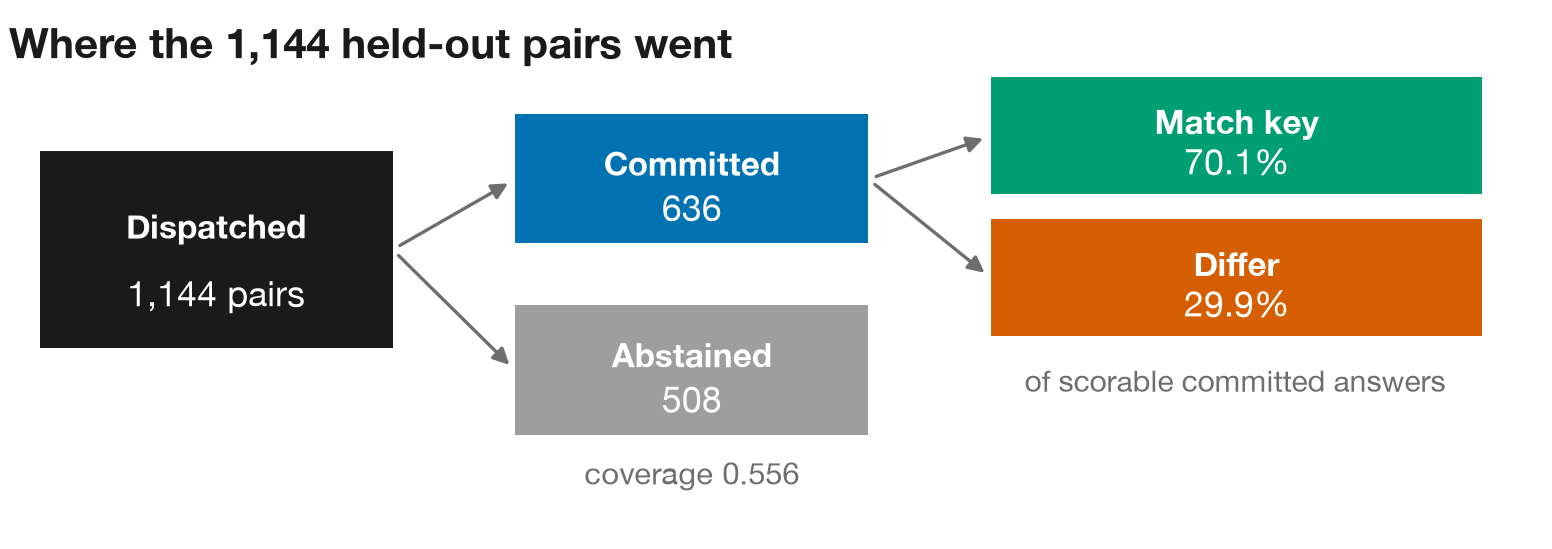
\includegraphics[width=6.1in,height=2.1578in]{media/media/image24.png}

@@CL@@Figure J.1: Where the 1,144 evaluation pairs went. 636 committed and 508 abstained, and of the scoreable commits 70.1\% match the published key.@@/CL@@

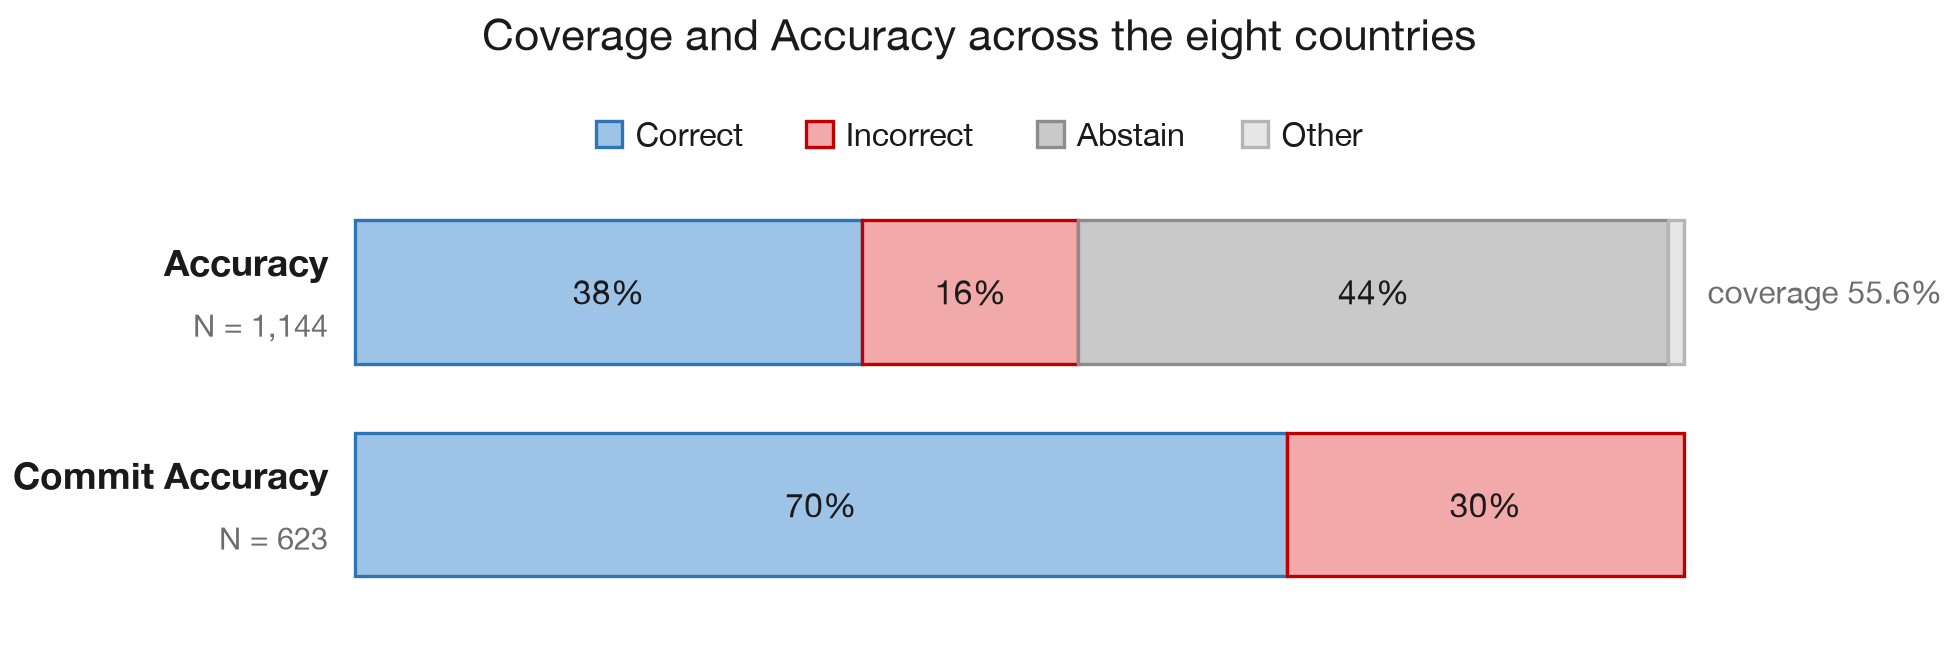
\includegraphics[width=6.1in,height=2.03126in]{media/media/image25.png}

@@CL@@Figure J.2: The evaluation run as shares of all 1,144 pairs, then of the 623 scoreable commits alone.@@/CL@@

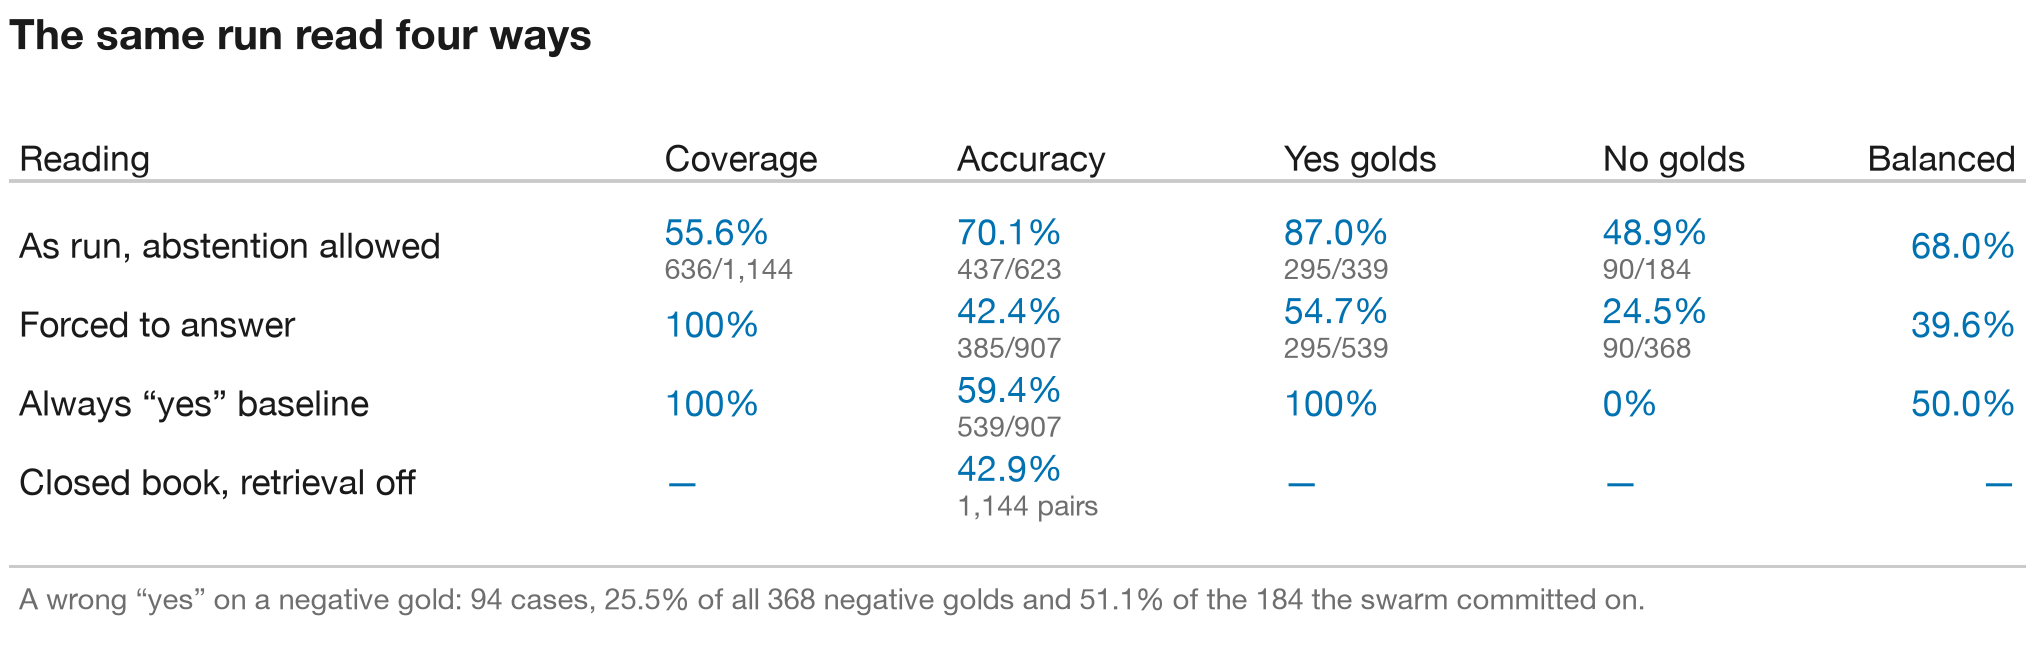
\includegraphics[width=6.1in,height=1.93641in]{media/media/image26.png}

@@CL@@Figure J.3: The same run read four ways. An alternative rendering of Table 4.1.1, with the negative-gold false-positive count underneath.@@/CL@@

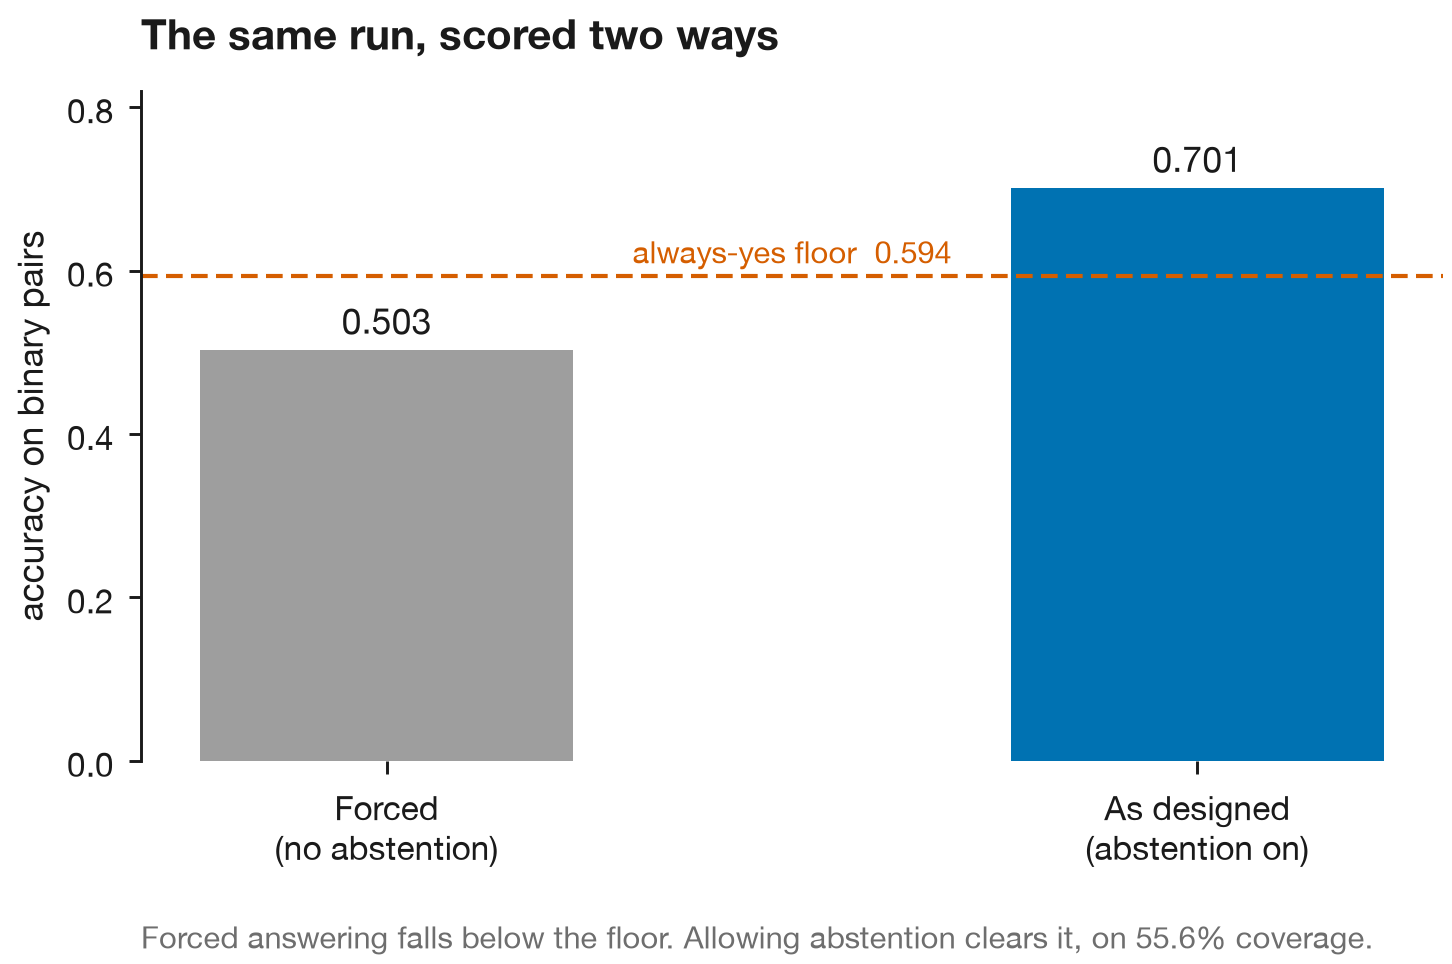
\includegraphics[width=6.09474in,height=4.04637in]{media/media/image27.png}

@@CL@@Figure J.4: Accuracy on binary pairs with abstention forced off and left on, against the always-yes floor of 0.594. Forced answering falls below the floor; allowing abstention clears it, on 55.6\% coverage.@@/CL@@

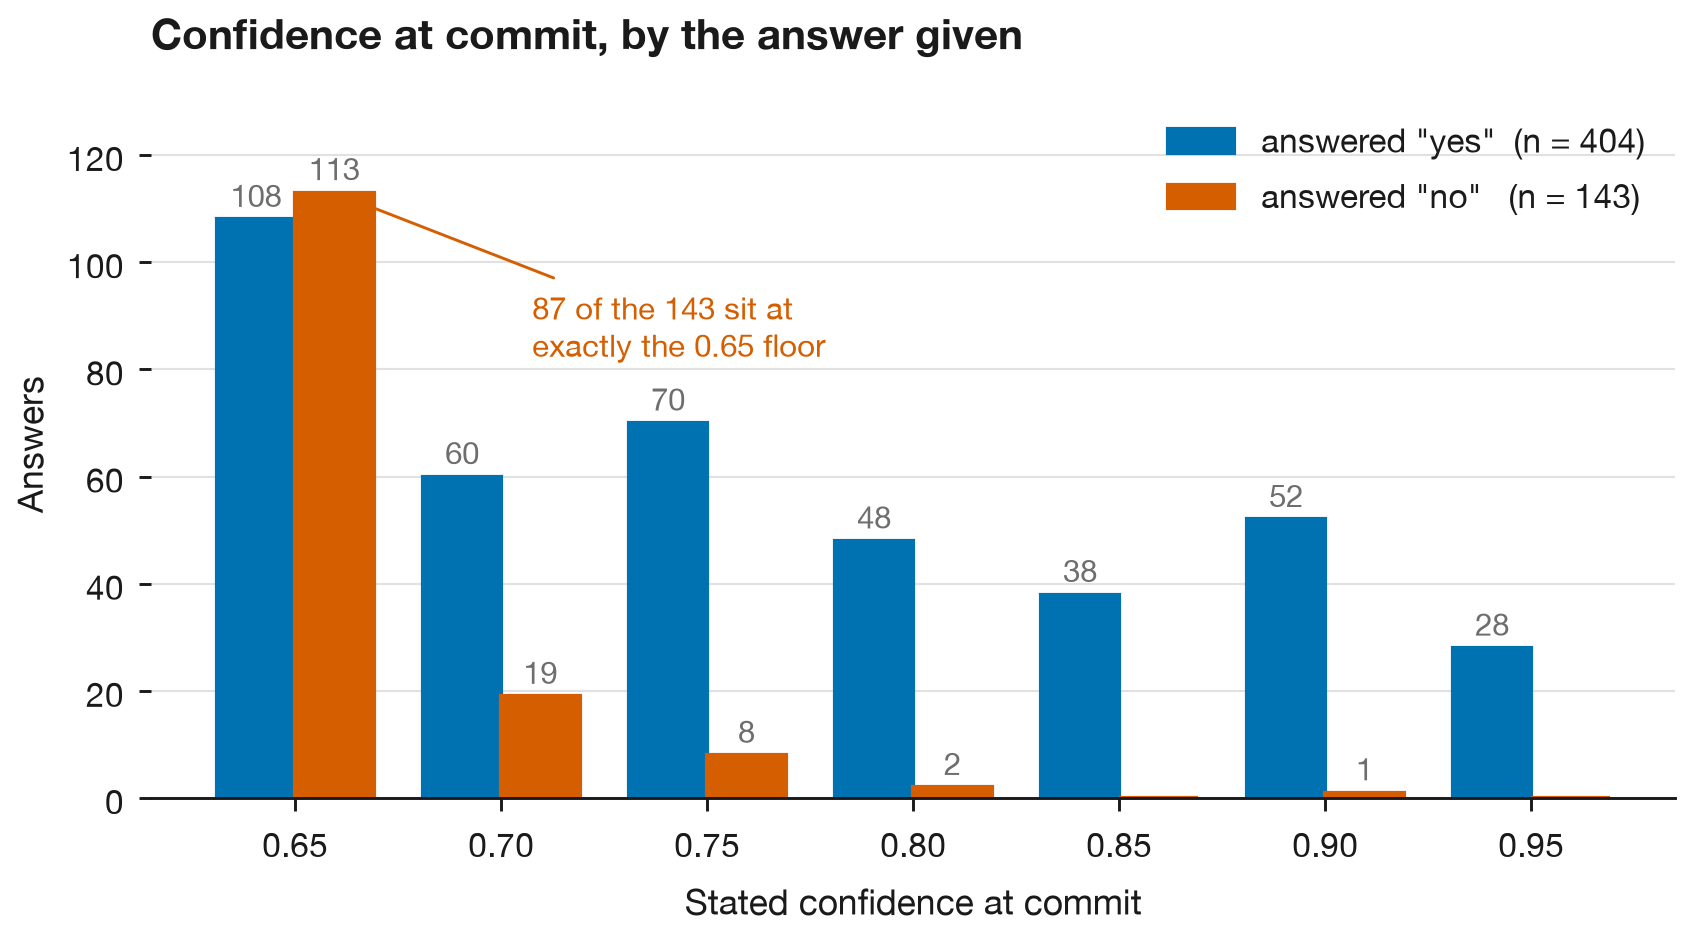
\includegraphics[width=6.1in,height=3.37239in]{media/media/image28.png}

@@CL@@Figure J.5: Stated confidence at the moment of commit, split by whether the swarm answered ``yes'' or ``no''. 87 of the 143 committed no answers sit at exactly the 0.65 floor.@@/CL@@

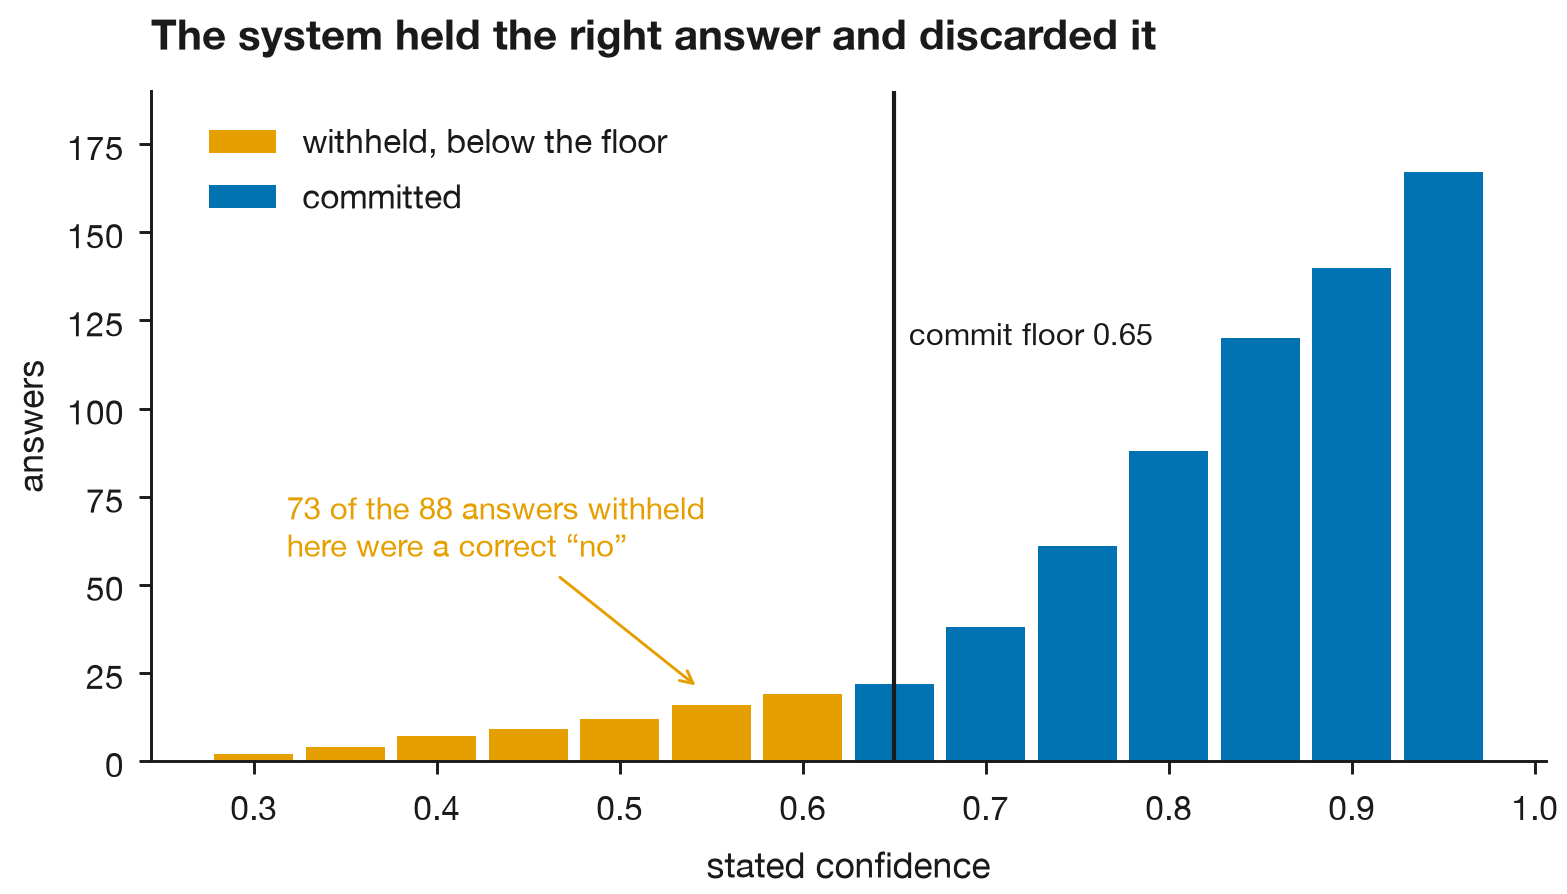
\includegraphics[width=6.1in,height=3.48015in]{media/media/image29.png}

@@CL@@Figure J.6: Answers held below the 0.65 commit floor beside those committed above it. 73 of the 88 withheld immediately under the floor were a correct no.@@/CL@@

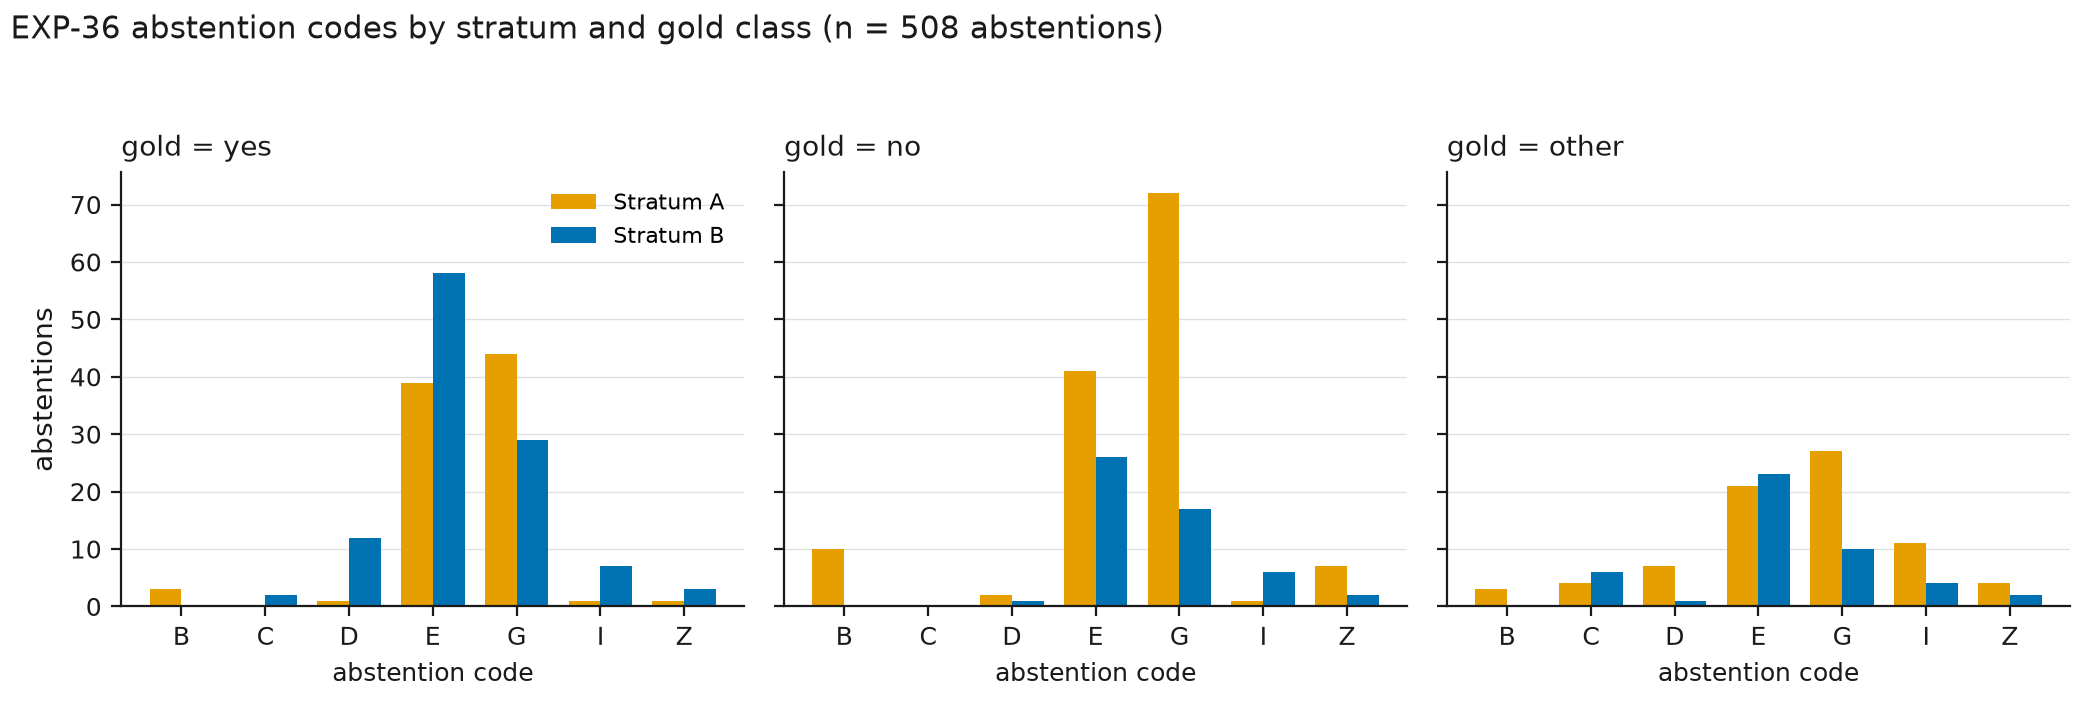
\includegraphics[width=6.1in,height=2.09143in]{media/media/image30.png}

@@CL@@Figure J.7: The 508 abstentions by code, split by resource stratum and by the class of the published answer.@@/CL@@

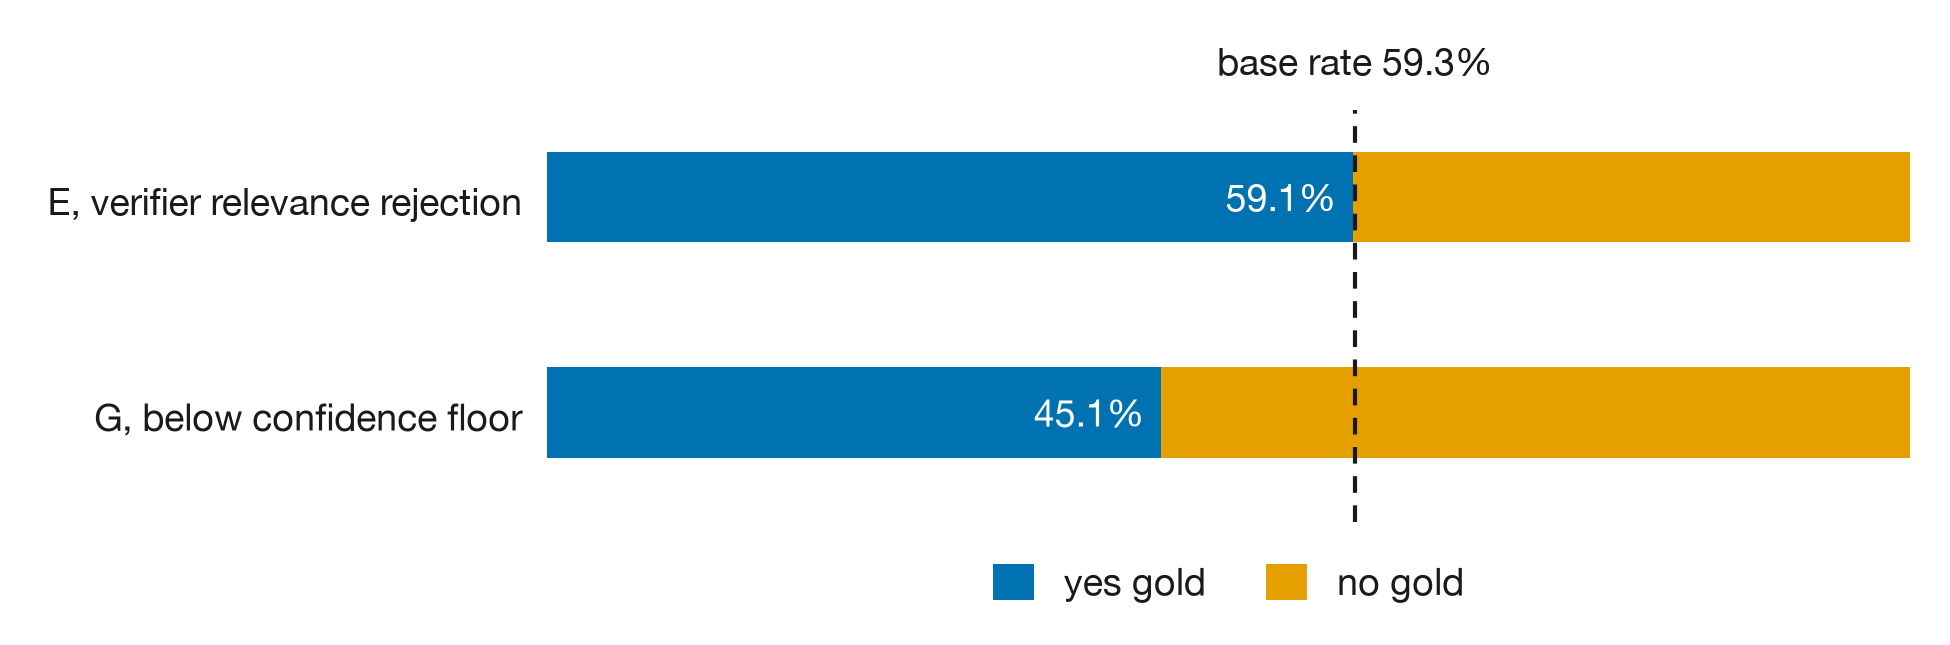
\includegraphics[width=6.1in,height=2.01769in]{media/media/image31.png}

@@CL@@Figure J.8: The gold-class mix of the two largest abstention codes against the evaluation base rate. Verifier rejections sit on the base rate at 59.1\%; floor failures are enriched in negative golds at 45.1\%.@@/CL@@

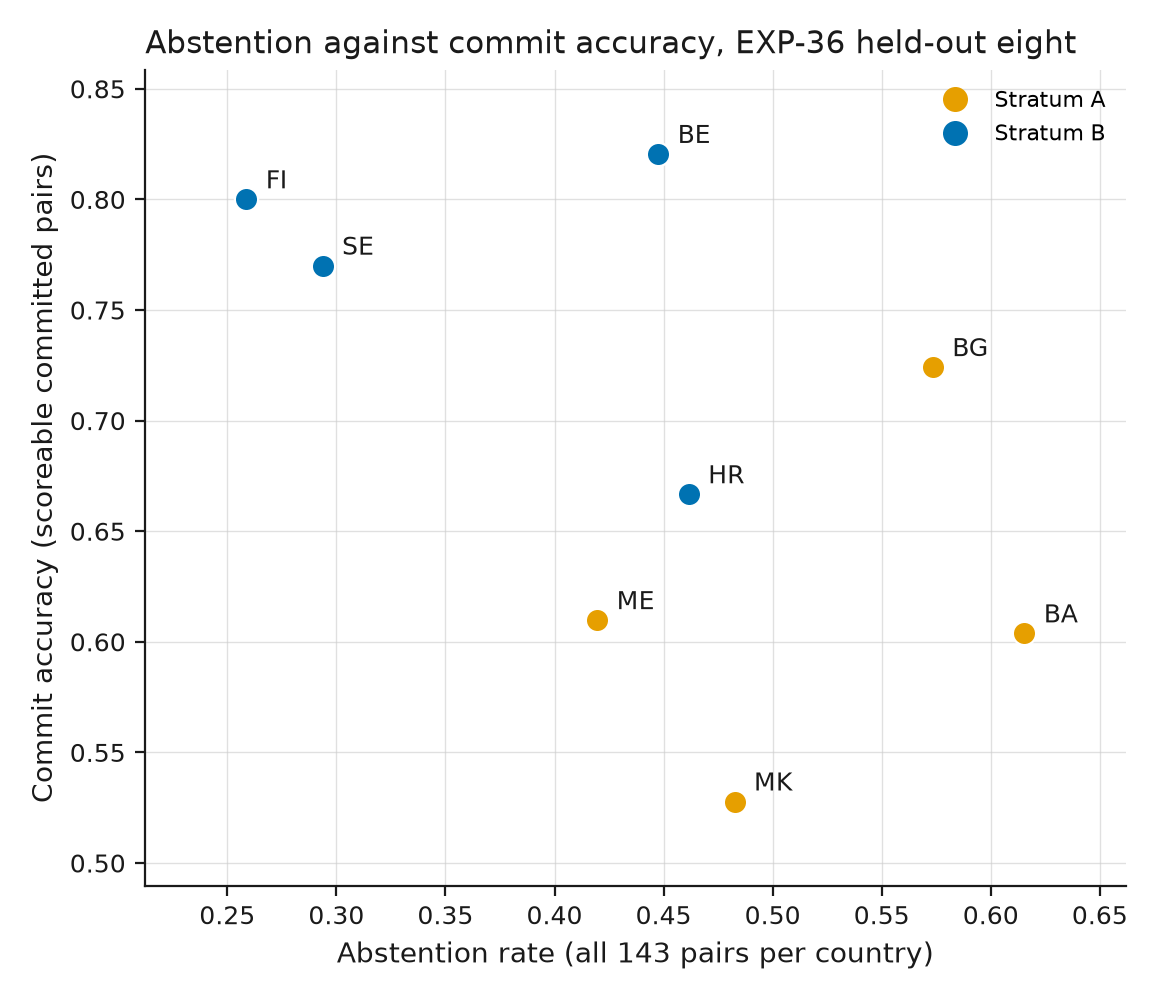
\includegraphics[width=4.69379in,height=4.04637in]{media/media/image32.png}

@@CL@@Figure J.9: Abstention rate against commit accuracy, one point per evaluation country. Abstaining more does not by itself buy accuracy.@@/CL@@

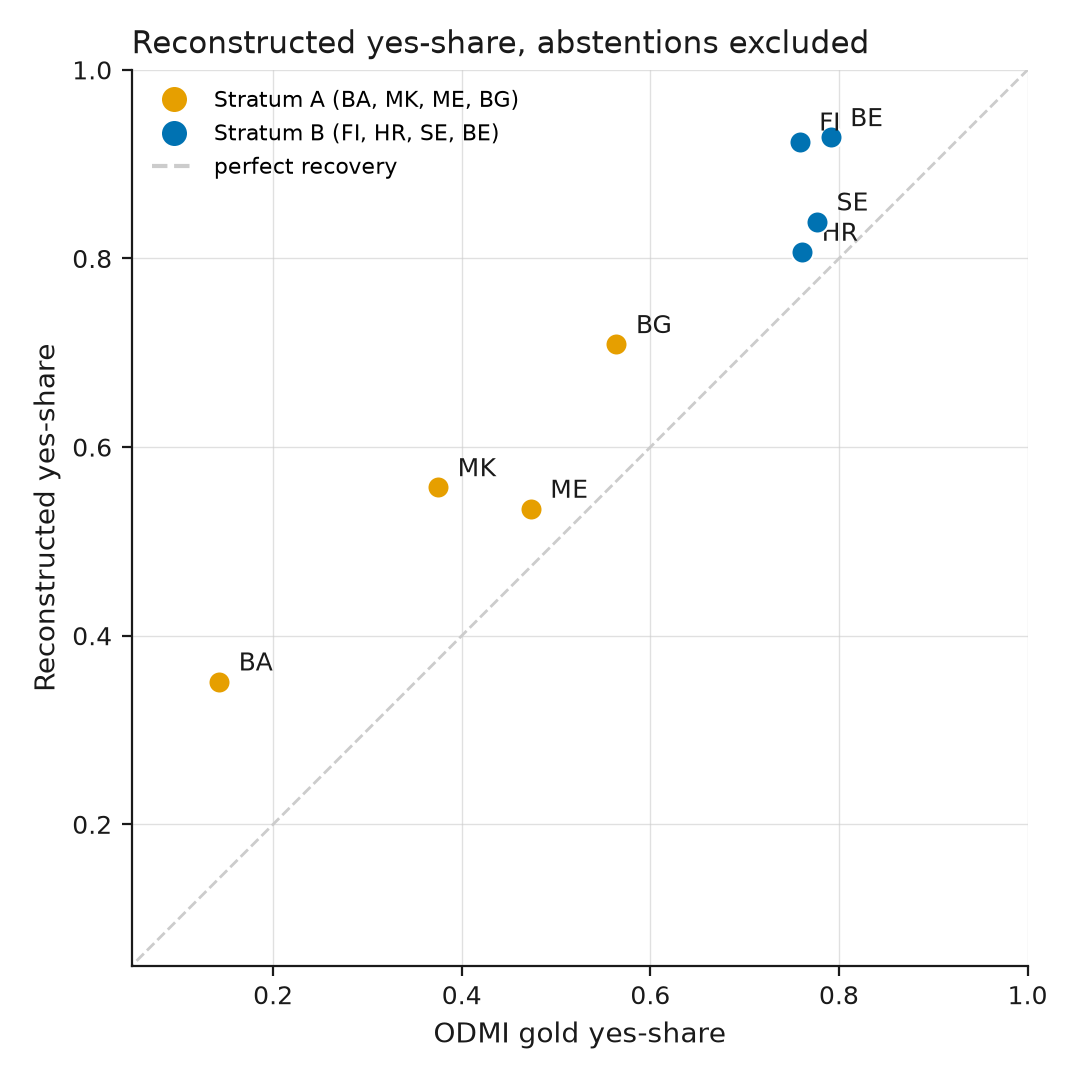
\includegraphics[width=4.04637in,height=4.04637in]{media/media/image33.png}

@@CL@@Figure J.10: Reconstructed yes-share against the published yes-share with abstentions dropped. Every country sits above the diagonal, so scoring only what the swarm answered overstates maturity.@@/CL@@

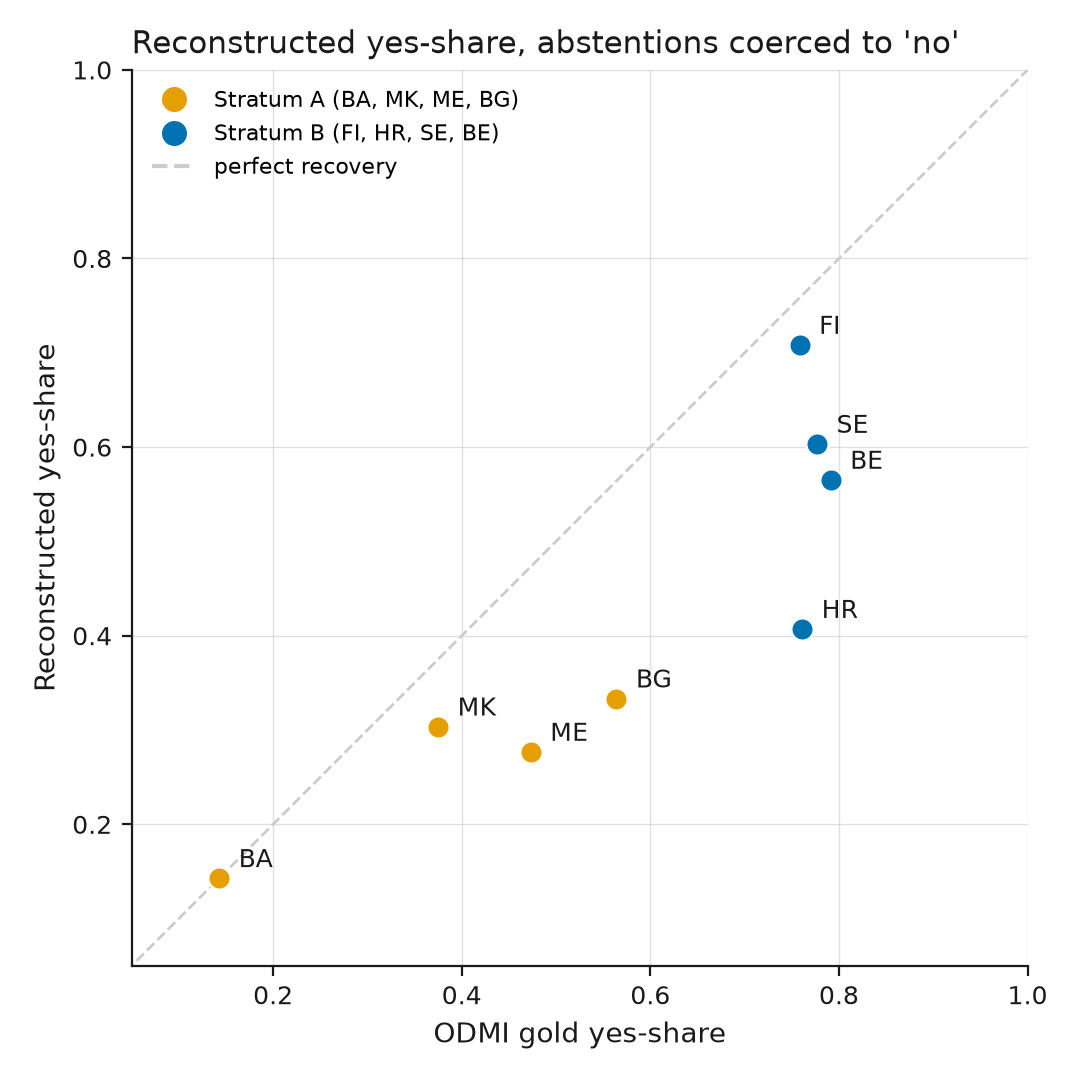
\includegraphics[width=4.04637in,height=4.04637in]{media/media/image34.png}

@@CL@@Figure J.11: The same reconstruction with every abstention coerced to no. The bias reverses and every country falls below the diagonal.@@/CL@@

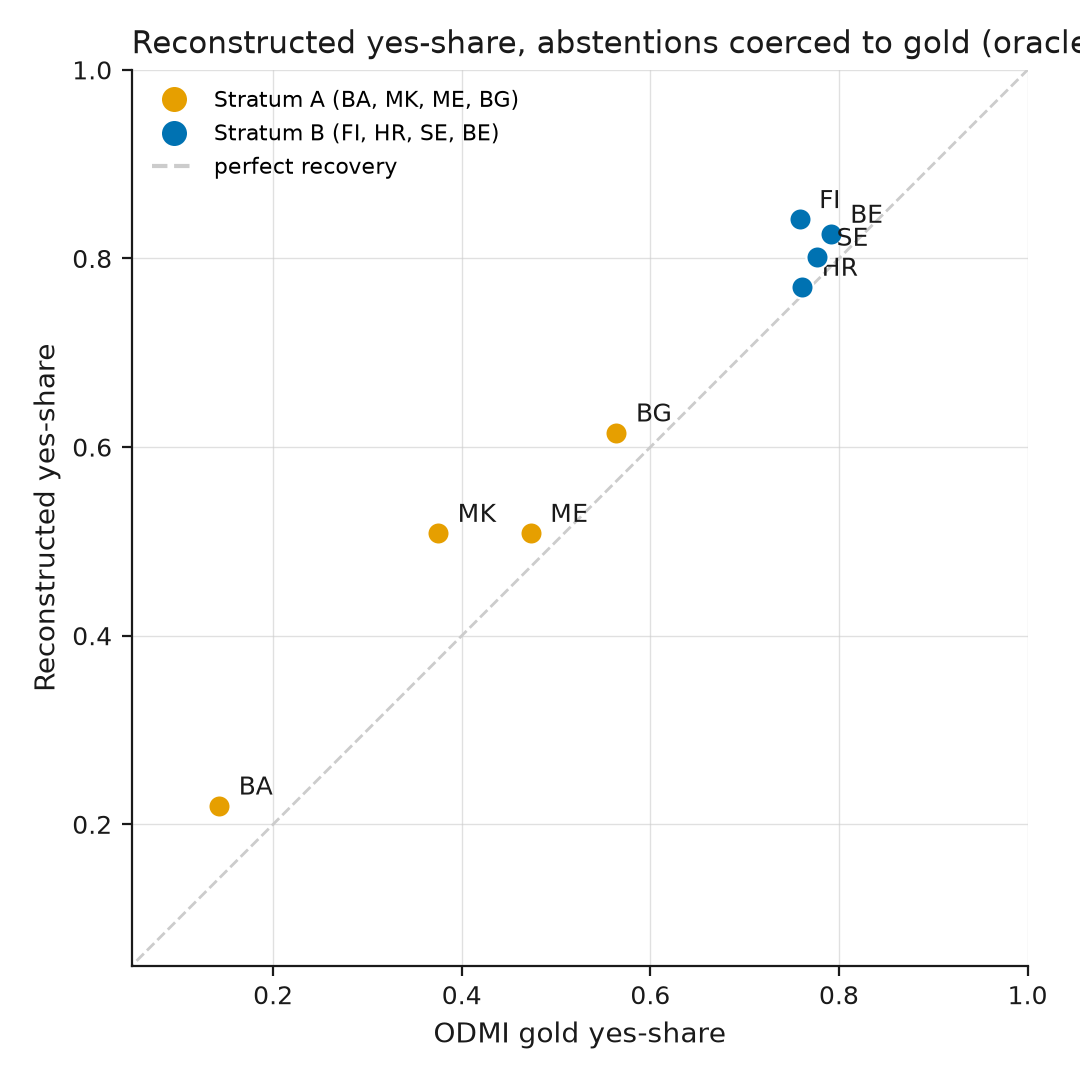
\includegraphics[width=4.04637in,height=4.04637in]{media/media/image35.png}

@@CL@@Figure J.12: The same reconstruction with abstentions filled from the published key. This is an oracle, and the ceiling the reconstruction would reach if abstention were solved.@@/CL@@

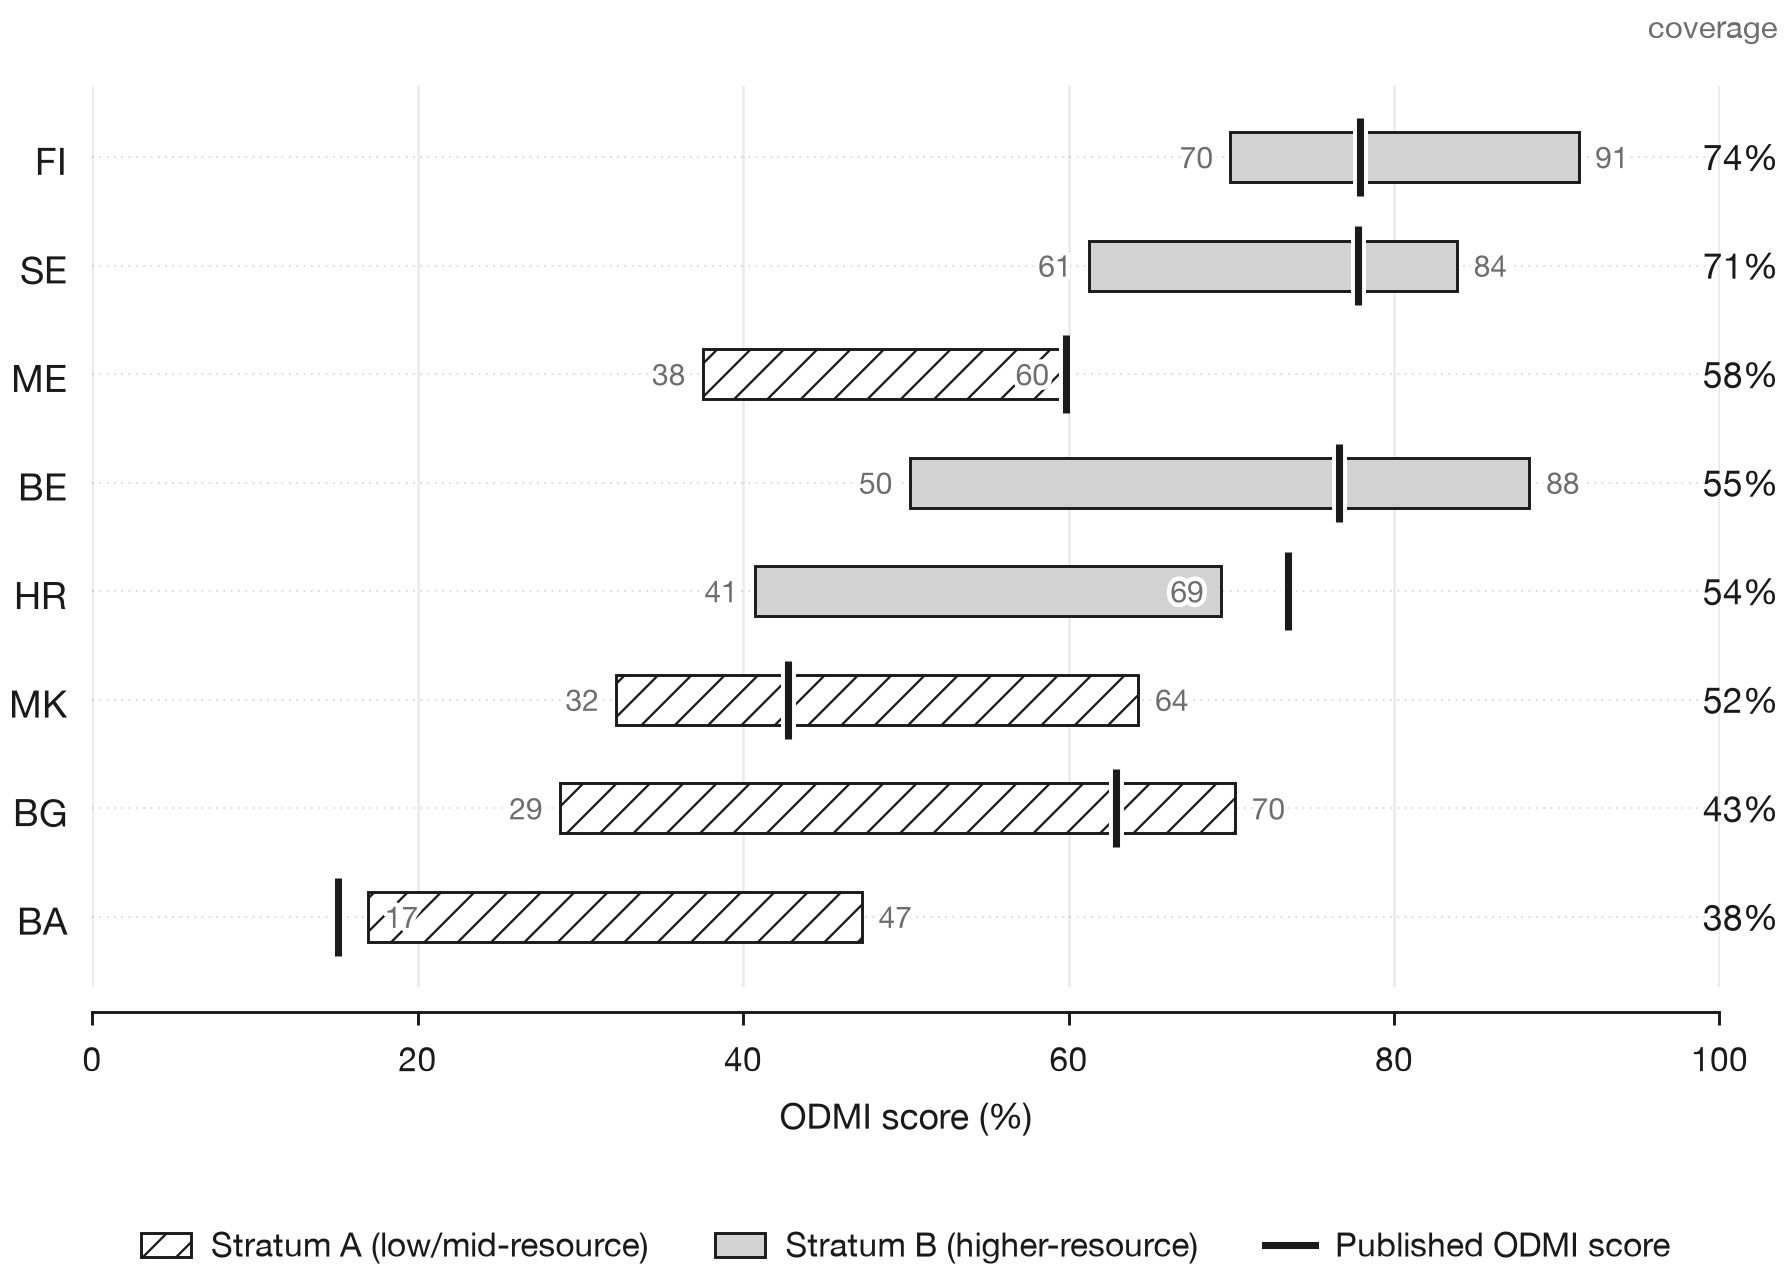
\includegraphics[width=5.61961in,height=4.04637in]{media/media/image36.png}

@@CL@@Figure J.13: The band each country\textquotesingle s reconstructed score could occupy, from treating every abstention as no to treating every one as yes, against the published score. Coverage is on the right.@@/CL@@

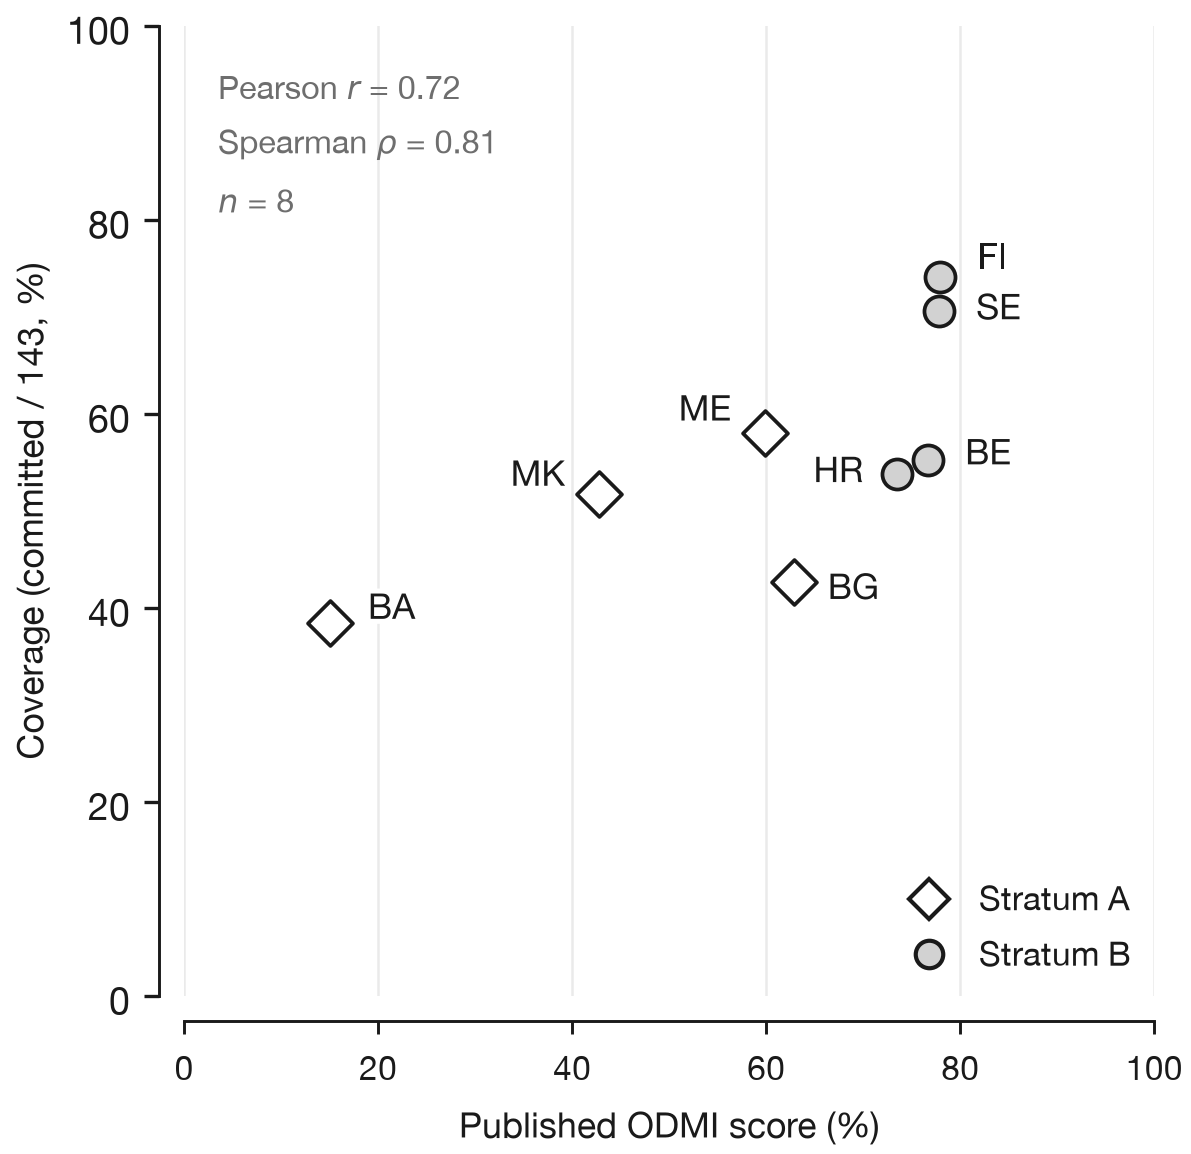
\includegraphics[width=4.17611in,height=4.04637in]{media/media/image37.png}

@@CL@@Figure J.14: Coverage against published ODMI score, one point per evaluation country, Pearson r 0.72 and Spearman rho 0.81 on eight points.@@/CL@@

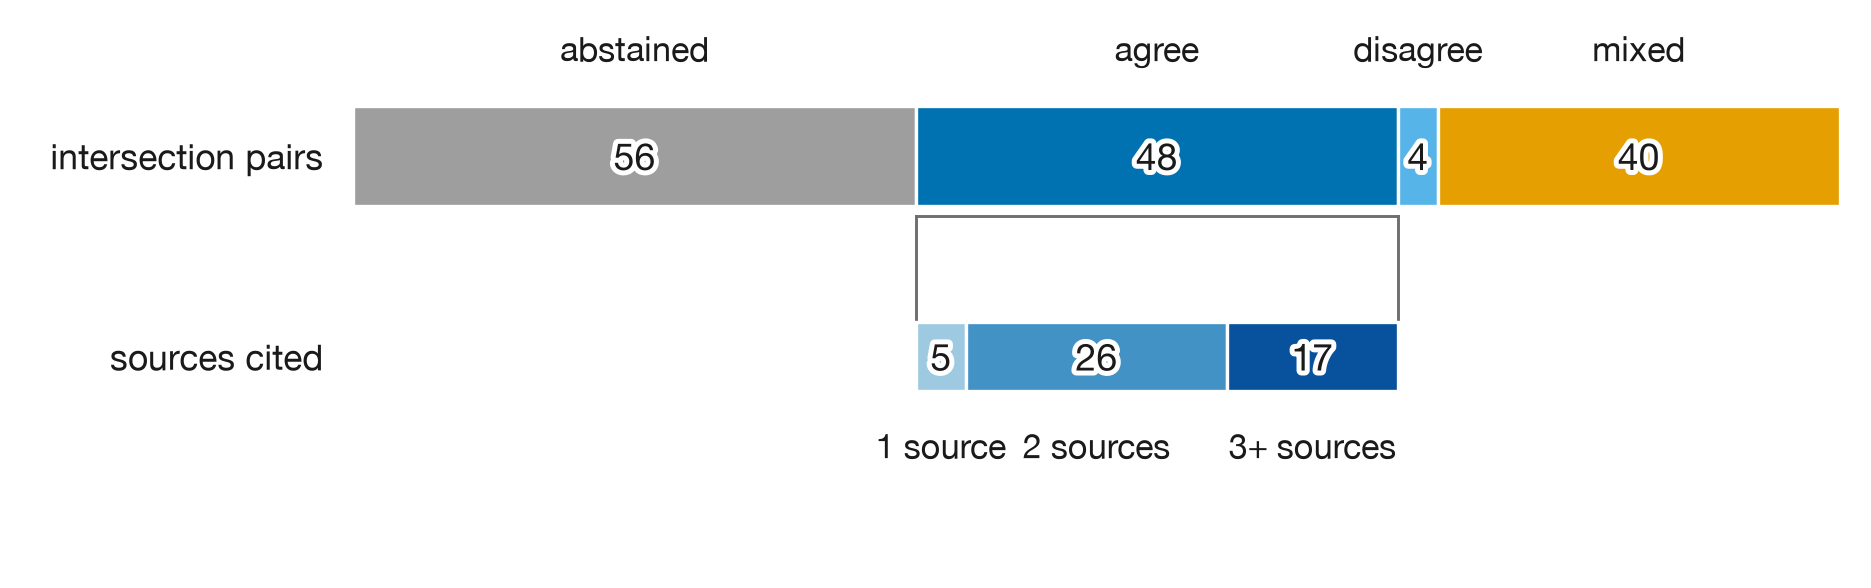
\includegraphics[width=6.1in,height=2.58382in]{media/media/image38.png}

@@CL@@Figure J.16: The two populations a human reviewer inherits. Declined answers arrive flagged and are easy to route; committed answers are identical in form whether right or wrong.@@/CL@@

@@CC@@The counts are not the evaluation run. They are the projection §4.8 makes over the full 5,148-pair questionnaire, where the evaluation coverage and commit accuracy put around 2,860 pairs committed and 2,290 declined, of which 2,010 right and 850 wrong.@@/CC@@

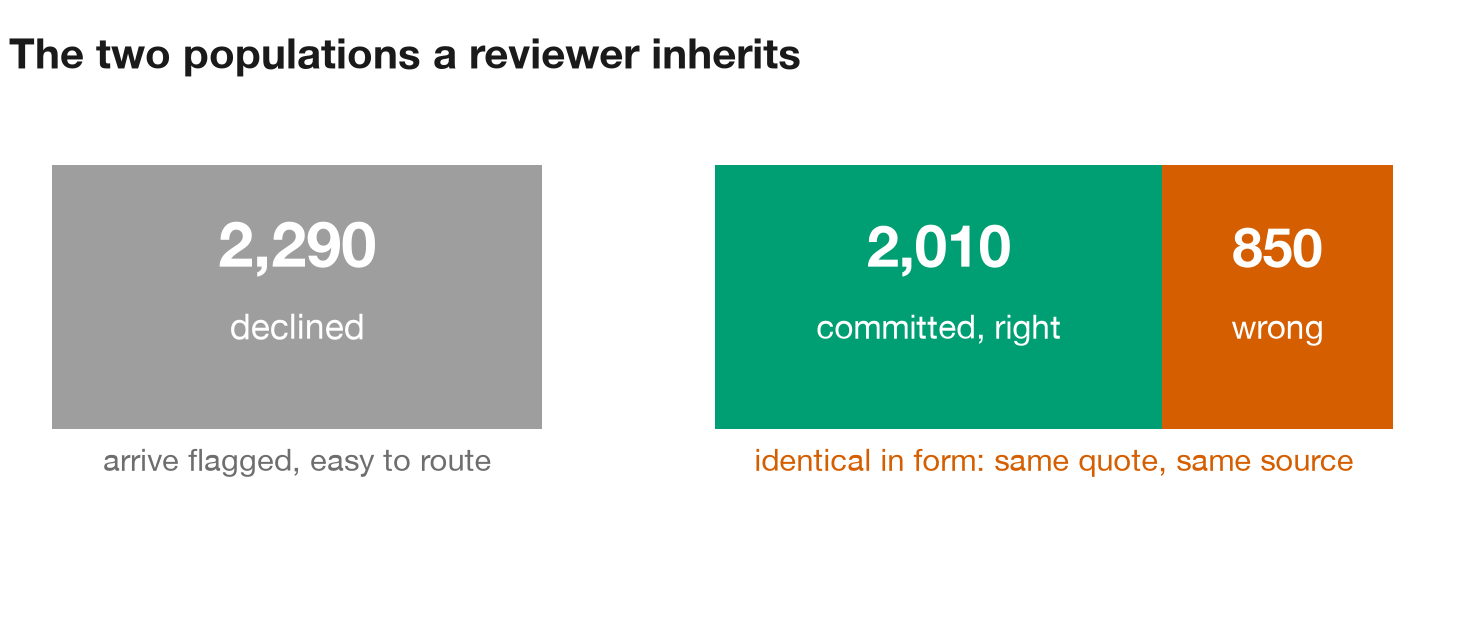
\includegraphics[width=6.1in,height=2.56865in]{media/media/image39.png}

@@CL@@Figure J.17: Why a ``yes'' and a ``no'' are not symmetric. A yes has a document behind it; a ``no'' rests on an absence, which leaves nothing to quote.@@/CL@@


\end{document}
